% Options for packages loaded elsewhere
\PassOptionsToPackage{unicode}{hyperref}
\PassOptionsToPackage{hyphens}{url}
%
\documentclass[
  11pt,
  french,
  a4paper,
  openany]{book}
\usepackage{lmodern}
\usepackage{amssymb,amsmath}
\usepackage{ifxetex,ifluatex}
\ifnum 0\ifxetex 1\fi\ifluatex 1\fi=0 % if pdftex
  \usepackage[T1]{fontenc}
  \usepackage[utf8]{inputenc}
  \usepackage{textcomp} % provide euro and other symbols
\else % if luatex or xetex
  \usepackage{unicode-math}
  \defaultfontfeatures{Scale=MatchLowercase}
  \defaultfontfeatures[\rmfamily]{Ligatures=TeX,Scale=1}
\fi
% Use upquote if available, for straight quotes in verbatim environments
\IfFileExists{upquote.sty}{\usepackage{upquote}}{}
\IfFileExists{microtype.sty}{% use microtype if available
  \usepackage[]{microtype}
  \UseMicrotypeSet[protrusion]{basicmath} % disable protrusion for tt fonts
}{}
\makeatletter
\@ifundefined{KOMAClassName}{% if non-KOMA class
  \IfFileExists{parskip.sty}{%
    \usepackage{parskip}
  }{% else
    \setlength{\parindent}{0pt}
    \setlength{\parskip}{6pt plus 2pt minus 1pt}}
}{% if KOMA class
  \KOMAoptions{parskip=half}}
\makeatother
\usepackage{xcolor}
\IfFileExists{xurl.sty}{\usepackage{xurl}}{} % add URL line breaks if available
\IfFileExists{bookmark.sty}{\usepackage{bookmark}}{\usepackage{hyperref}}
\hypersetup{
  pdftitle={Cours de chimie générale},
  pdfauthor={M. Michele Rizzello; Mme Émilie Pittet},
  pdflang={fr},
  hidelinks,
  pdfcreator={LaTeX via pandoc}}
\urlstyle{same} % disable monospaced font for URLs
\usepackage[margin=1in]{geometry}
\usepackage{longtable,booktabs}
% Correct order of tables after \paragraph or \subparagraph
\usepackage{etoolbox}
\makeatletter
\patchcmd\longtable{\par}{\if@noskipsec\mbox{}\fi\par}{}{}
\makeatother
% Allow footnotes in longtable head/foot
\IfFileExists{footnotehyper.sty}{\usepackage{footnotehyper}}{\usepackage{footnote}}
\makesavenoteenv{longtable}
\usepackage{graphicx,grffile}
\makeatletter
\def\maxwidth{\ifdim\Gin@nat@width>\linewidth\linewidth\else\Gin@nat@width\fi}
\def\maxheight{\ifdim\Gin@nat@height>\textheight\textheight\else\Gin@nat@height\fi}
\makeatother
% Scale images if necessary, so that they will not overflow the page
% margins by default, and it is still possible to overwrite the defaults
% using explicit options in \includegraphics[width, height, ...]{}
\setkeys{Gin}{width=\maxwidth,height=\maxheight,keepaspectratio}
% Set default figure placement to htbp
\makeatletter
\def\fps@figure{htbp}
\makeatother
\setlength{\emergencystretch}{3em} % prevent overfull lines
\providecommand{\tightlist}{%
  \setlength{\itemsep}{0pt}\setlength{\parskip}{0pt}}
\setcounter{secnumdepth}{5}
\widowpenalty10000
\clubpenalty10000

\usepackage{tcolorbox}
\newtcolorbox{objectives}{
  standard jigsaw,
  opacityback=0,
  colframe=black,
  boxrule=1pt}

\renewcommand{\arraystretch}{1.5}

\usepackage{multicol}

\usepackage{booktabs}
\usepackage{amsthm}
\usepackage{cancel}
\usepackage{gensymb}
\usepackage[version=4]{mhchem}
\usepackage{tabto}

\usepackage[answerdelayed,lastexercise]{exercise}
\renewcommand{\ExerciseName}{Exercice}
\renewcommand{\AnswerName}{Solution de l'exercice}

\usepackage{fancyhdr}
\setlength{\headheight}{14pt}
\pagestyle{fancy}
\lhead{}
\chead{}
\rhead{\leftmark}
\lfoot{GNLC - 2021/2022}
\cfoot{}
\rfoot{\thepage}
\renewcommand{\headrulewidth}{0.2pt}
\renewcommand{\footrulewidth}{0.2pt}
\renewcommand{\chaptermark}[1]{\markboth{\thechapter.\space#1}{}}

\makeatletter
\def\thm@space@setup{%
  \thm@preskip=8pt plus 2pt minus 4pt
  \thm@postskip=\thm@preskip
}
\makeatother

\newenvironment{credit}
  {\vspace{-2em}\begin{center}\begin{footnotesize}\begin{textit}}
  {\end{textit}\end{footnotesize}\end{center}}
\ifxetex
  % Load polyglossia as late as possible: uses bidi with RTL langages (e.g. Hebrew, Arabic)
  \usepackage{polyglossia}
  \setmainlanguage[]{french}
\else
  \usepackage[shorthands=off,main=french]{babel}
\fi

\title{Cours de chimie générale}
\author{M. Michele Rizzello \and Mme Émilie Pittet}
\date{25.06.2022}

\begin{document}
\maketitle

{
\setcounter{tocdepth}{1}
\tableofcontents
}
\hypertarget{pruxe9ambule}{%
\chapter*{Préambule}\label{pruxe9ambule}}
\addcontentsline{toc}{chapter}{Préambule}

\textbf{Cours de chimie Générale} édité par les enseignants du gymnase de Nyon la Côte.

Ce manuel fournit aux étudiants (OS et DF) les connaissances de base nécessaires en chimie pour l'obtention du certificat de maturité gymnasiale. Il sert de support de cours pour l'accompagnement des leçons et des travaux pratiques proposés en classe.

Le document est en cours de rédaction et des ajouts ou modifications peuvent avoir lieu en cours d'année scolaire. Chaque révision visera à améliorer la qualité et la précision du contenu et à souligner sa pertinence pour les étudiants.

Le contenu est disponible en ligne au format HTML à l'url \url{www.chimie-generale.ch}, adresse à laquelle il est également possible de télécharger le contenu au format PDF ou EPUB (format standardisé pour les livres numériques). Le document est édité en utilisant la technologie \href{https://bookdown.org/}{bookdown} qui permet de rédiger des livres HTML, PDF, ePub en utilisant la syntaxe R Markdown.

Ce projet est ouvert aux contributions et aux suggestions. Si vous souhaitez participer à son amélioration, le code source est disponible sur la plateforme GitHub à l'adresse \url{https://github.com/mrizzello/chimie-generale}. Nous serions heureux de faire évoluer ce document vers un projet participatif de plus grande ampleur. Vous pouvez créer une \emph{Pull Request} ou une \emph{Issue} sur GitHub et nous l'examinerons dès que possible.

\vspace{\stretch{1}}


\includegraphics{images/by-nc-sa.png}
Cet ouvrage est placé sous licence Creative Commons \href{https://creativecommons.org/licenses/by-sa/4.0/deed.fr}{CC BY-SA 4.0}.

En tant que ressource éducative libre, vous pouvez modifier ou distribuer ce document selon les conditions énoncées par la licence Creative Commons. Développé à l'origine dans le cadre du cours de chimie générale pour l'obtention du certificat de maturité gymnasiale du gymnase de Nyon - la Côte.

\hypertarget{introduction}{%
\chapter{Introduction}\label{introduction}}

\begin{tcolorbox}
\textbf{Chimie}\\
La chimie est la science qui étudie la composition, les propriétés et les transformations de la matière.

\end{tcolorbox}

Comme celle énoncée ci-dessus, les définitions de la chimie incluent généralement les termes: matière, composition, propriété et transformation.

\textbf{La matière est tout ce qui a une masse et qui occupe l'espace.} Tous les objets que nous voyons autour de nous sont constitués de matière. Les gaz qui constituent l'atmosphère, même si ils sont invisibles, sont de la matière. Ils occupent l'espace et ils ont une masse.

Le terme \textbf{composition} se réfère aux composants d'un échantillon de matière. L'air que nous respirons est un mélange composé d'environ \(3/4\) d'azote et \(1/4\) d'oxygène et la formule chimique de l'eau H\textsubscript{2}O nous indique qu'elle est composée d'hydrogène et d'oxygène.

Les \textbf{propriétés} sont des caractéristiques qui nous permettent de distinguer un échantillon de matière d'un autre échantillon. Un morceau de fer fondra à 1538 °C, alors qu'un glaçon fondra à 0 °C.

\hypertarget{propriuxe9tuxe9s-et-transformations}{%
\section{Propriétés et transformations}\label{propriuxe9tuxe9s-et-transformations}}

Pour étudier la matière, nous allons nous intéresser à deux types de \textbf{propriétés} et aux deux types de \textbf{transformations} que la matière peut subir.

\hypertarget{propriuxe9tuxe9s-physiques}{%
\subsection{Propriétés physiques}\label{propriuxe9tuxe9s-physiques}}

Les propriétés physiques sont des caractéristiques qui ne changent pas la composition de la matière (la couleur, la densité, le point de fusion, le point d'ébullition, la dureté, etc.).

\hypertarget{propriuxe9tuxe9s-chimiques}{%
\subsection{Propriétés chimiques}\label{propriuxe9tuxe9s-chimiques}}

Les propriétés chimiques sont des caractéristiques qui changent la composition de la matière. Elles décrivent la façon dont une substance peut se transformer pour former d'autres substances (l'inflammabilité, la corrosivité, la réactivité avec des acides, etc.).

\hypertarget{transformations-physiques}{%
\subsection{Transformations physiques}\label{transformations-physiques}}

Lors d'une \textbf{transformation physique}, la matière change son apparence physique, mais pas sa composition. On retrouve la même substance avant et après la transformation. L'évaporation de l'eau est une transformation physique. Lorsque l'eau s'évapore, elle passe de l'état liquide à l'état gazeux, mais elle est toujours constituée de molécules d'eau.

\[ \underset{\text{évaporation}}{\text{eau à l'état liquide} \ \longrightarrow \ \text{eau à l'état gazeux}} \]

\hypertarget{transformations-chimiques}{%
\subsection{Transformations chimiques}\label{transformations-chimiques}}

Lors d'une \textbf{transformation chimique}, la matière est transformée en une autre substance dont la composition est différente. La composition de la matière est différente avant et après la transformation. La combustion du papier est une transformation chimique. Le papier et l'oxygène de l'air réagissent ensemble pour former du dioxyde de carbone et de l'eau.

\[ \underset{\text{combustion}}{\text{papier}\ +\ \text{oxygène} \ \longrightarrow \ \text{dioxyde de carbone} + \text{eau}} \]

Les transformations chimiques sont ce que nous appellerons plus tard des \textbf{réactions chimiques}.

\begin{Exercise}
En essayant de caractériser une substance, un chimiste observe les propriétés suivantes:

\begin{itemize}
\tightlist
\item
  La substance est un métal blanc argenté brillant.
\item
  La substance fond à 649° C et bout à 1105° C.
\item
  La densité de la substance à 20° C est de 1.738 {[}g/cm\(^3\){]}.
\item
  La substance brûle au contact de l'air, produisant une lumière blanche intense.
\item
  La substance réagit avec le chlore pour donner un solide blanc cassant.
\item
  La substance peut être martelée en feuilles minces ou étirée en fils.
\item
  La substance est un bon conducteur de l'électricité.
\end{itemize}

Lesquelles de ces caractéristiques sont des propriétés physiques, et lesquelles sont des propriétés chimiques?

\end{Exercise}

\begin{Answer}

\begin{itemize}
\tightlist
\item
  La substance est un métal blanc argenté brillant.\\
  \textbf{propriété physique}
\item
  La substance fond à 649° C et bout à 1105° C.\\
  \textbf{propriété physique}
\item
  La densité de la substance à 20° C est de 1.738 {[}g/cm\(^3\){]}.\\
  \textbf{propriété physique}
\item
  La substance brûle au contact de l'air, produisant une lumière blanche intense.\\
  \textbf{propriété chimique}
\item
  La substance réagit avec le chlore pour donner un solide blanc cassant.\\
  \textbf{propriété chimique}
\item
  La substance peut être martelée en feuilles minces ou étirée en fils.\\
  \textbf{propriété physique}
\item
  La substance est un bon conducteur de l'électricité.\\
  \textbf{propriété physique}
\end{itemize}


\end{Answer}

\hypertarget{systuxe8me-de-mesure}{%
\section{Système de mesure}\label{systuxe8me-de-mesure}}

La chimie est une science qui se base sur des résultats expérimentaux ou des théories qui ont pour point de départ l'observation. La plupart de ces observations sont faites de manières \textbf{quantitatives} : ce sont des mesures.

Un système de mesure universel, le Système International (SI) a été adopté en 1960 par la Conférence Générale des Poids et Mesures. Le SI comporte sept unités de base.

\begin{longtable}[]{@{}lcl@{}}
\caption{\label{tab:tab-SIunits} Unités de base du Système International.}\tabularnewline
\toprule
Unité SI & Symbole & Grandeur\tabularnewline
\midrule
\endfirsthead
\toprule
Unité SI & Symbole & Grandeur\tabularnewline
\midrule
\endhead
le \textbf{mètre} & m & unité de longueur\tabularnewline
la \textbf{seconde} & s & unité de temps\tabularnewline
le \textbf{kilogramme} & kg & unité de masse\tabularnewline
l'\textbf{ampère} & A & unité d'intensité des courants électriques\tabularnewline
le \textbf{kelvin} & K & unité de température\tabularnewline
la \textbf{candela} & cd & unité d'intensité lumineuse\tabularnewline
la \textbf{mole} & mol & unité de quantité de matière\tabularnewline
\bottomrule
\end{longtable}

\hypertarget{les-puissances-de-10}{%
\section{Les puissances de 10}\label{les-puissances-de-10}}

Dans le domaine des sciences expérimentales, il est très commode d'exprimer une valeur numérique, souvent très grande ou très petite sous forme d'un produit de deux facteurs: un nombre compris entre 1 et 10 et une puissance de 10. Cette notation est appelée \textbf{notation scientifique}.

Rappel :

\[ \begin{split}
    1 &= 10^0\\
    10 &= 10^1\\
    100 &= 10^2\\
    1000 &= 10^3\\
    10000 &= 10^4
\end{split}
\qquad
\begin{split}
    \\
    0.1 &= 10^{-1}\\
    0.01 &= 10^{-2}\\
    0.001 &= 10^{-3}\\
    0.0001 &= 10^{-4}
\end{split} \]

Exemples de notation scientifique :

\[ \begin{split}
    4564 &= 4.564\cdot10^3\\
    212575000000 &= 2.12575\cdot10^{11}\\
    0.000007567 &= 7.567\cdot10^{-6}\\
    0.00000000000000785 &= 7.85\cdot10^{-15}\\
\end{split} \]

Deux relations importantes à retenir :

\[ \begin{split}
    10^a \cdot 10^b = 10^{(a+b)}
\end{split}
\qquad
\begin{split}
    \frac{10^a}{10^b} = 10^{(a-b)}
\end{split} \]

\begin{Exercise}
Exprimez les valeurs numériques suivantes en notation réelle ou en notation scientifique

\end{Exercise}

\begin{longtable}[]{@{}cc@{}}
\toprule
notation réelle & notation scientifique\tabularnewline
\midrule
\endhead
\(17.9915\) &\tabularnewline
& \(3.756 \cdot 10^{4}\)\tabularnewline
\(0.00034159\) &\tabularnewline
& \(13.365 \cdot 10^{-5}\)\tabularnewline
& \(103.351 \cdot 10 ^{2}\)\tabularnewline
\(14896.546\) &\tabularnewline
\bottomrule
\end{longtable}

\begin{Answer}
\(17.9915\) = \(1.79915 \cdot 10^{1}\)

\(37560\) = \(3.756 \cdot 10^{4}\)

\(0.00034159\) = \(3.4159 \cdot 10^{-4}\)

\(0.00013365\) = \(13.365 \cdot 10^{-5}\)

\(10335.1\) = \(103.351 \cdot 10 ^{2}\)

\(14896.546\) = \(1.4896546 \cdot 10^{4}\)

\end{Answer}

\hypertarget{multiples-des-unituxe9s}{%
\section{Multiples des unités}\label{multiples-des-unituxe9s}}

\begin{longtable}[]{@{}cccccc@{}}
\caption{\label{tab:tab-SImultiples} Multiples et sous-multiples décimaux des unités du système international (SI).}\tabularnewline
\toprule
Facteur & Préfixe SI & Symbole SI & Facteur & Préfixe SI & Symbole SI\tabularnewline
\midrule
\endfirsthead
\toprule
Facteur & Préfixe SI & Symbole SI & Facteur & Préfixe SI & Symbole SI\tabularnewline
\midrule
\endhead
\(10^{-1}\) & déci & d & \(10\) & déca & da\tabularnewline
\(10^{-2}\) & centi & c & \(10^{2}\) & hecto & h\tabularnewline
\(10^{-3}\) & milli & m & \(10^{3}\) & kilo & k\tabularnewline
\(10^{-6}\) & micro & \(\mu\) & \(10^{6}\) & mega & M\tabularnewline
\(10^{-9}\) & nano & n & \(10^{9}\) & giga & G\tabularnewline
\(10^{-12}\) & pico & p & \(10^{12}\) & téra & T\tabularnewline
\(10^{-15}\) & femto & f & \(10^{15}\) & péta & P\tabularnewline
\(10^{-18}\) & atto & a & \(10^{18}\) & exa & E\tabularnewline
\bottomrule
\end{longtable}

\newpage

\begin{Exercise}

Répondez aux questions suivantes :

\begin{enumerate}
\def\labelenumi{\arabic{enumi}.}
\item
  Combien de milligrammes y a-t-il dans un kilogrammes ?
  \vspace{\stretch{1}}
\item
  Combien de nanomètres y a-t-il dans un mètre ?
  \vspace{\stretch{1}}
\item
  Combien y a-t-il de kilogrammes dans un microgramme ?
  \vspace{\stretch{1}}
\item
  Combien y a-t-il de microlitres dans un millilitre ?
  \vspace{\stretch{1}}
\end{enumerate}

Effectuez chacune des conversions d'unités suivantes :

\begin{enumerate}
\def\labelenumi{\arabic{enumi}.}
\setcounter{enumi}{4}
\tightlist
\item
  \(8.43\) {[}cm{]} en millimètres.
  \vspace{\stretch{1}}
\item
  \(2.41 \cdot 10^{2}\) {[}cm{]} en mètres.
  \vspace{\stretch{1}}
\item
  \(294.5\) {[}nm{]} en centimètres.
  \vspace{\stretch{1}}
\item
  \(1.445 \cdot 10^{4}\) {[}m{]} en kilomètres.
  \vspace{\stretch{1}}
\end{enumerate}


\end{Exercise}

\begin{Answer}

\begin{enumerate}
\def\labelenumi{\arabic{enumi}.}
\tightlist
\item
  \(10^{6}\) {[}mg{]}
\item
  \(10^{9}\) {[}nm{]}
\item
  \(10^{-9}\) {[}kg{]}
\item
  \(10^{3}\) {[}\(\mu\)l{]}
\item
  \(84.3\) {[}mm{]}
\item
  \(2.41\) {[}m{]}
\item
  \(2.945\cdot10^{-5}\) {[}cm{]}
\item
  \(14.45\) {[}km{]}
\end{enumerate}

\newpage


\end{Answer}

\hypertarget{exercices-suppluxe9mentaires}{%
\section{Exercices supplémentaires}\label{exercices-suppluxe9mentaires}}

\begin{Exercise}

Indiquez si les transformations suivantes sont des transformations physiques ou chimiques:

\begin{enumerate}
\def\labelenumi{\arabic{enumi}.}
\tightlist
\item
  Une boîte de conserve qui rouille.\\
\item
  L'ébullition d'une tasse d'eau.\\
\item
  La digestion d'une barre chocolatée.\\
\item
  Une explosion de nitroglycérine.\\
\item
  Le ternissement lent d'une fourchette en argent à l'air.
\end{enumerate}


\end{Exercise}

\begin{Answer}

\begin{enumerate}
\def\labelenumi{\arabic{enumi}.}
\tightlist
\item
  Une boîte de conserve qui rouille.\\
  \textbf{transformation chimique}
\item
  L'ébullition d'une tasse d'eau.\\
  \textbf{transformation physique}
\item
  La digestion d'une barre chocolatée.\\
  \textbf{transformation chimique}
\item
  Une explosion de nitroglycérine.\\
  \textbf{transformation chimique}
\item
  Le ternissement lent d'une fourchette en argent à l'air.\\
  \textbf{transformation chimique}
\end{enumerate}


\end{Answer}

\begin{Exercise}

Indiquez si les transformations suivantes sont des transformations physiques ou chimiques et indiquez quelle est la propriété observée:

\begin{enumerate}
\def\labelenumi{\arabic{enumi}.}
\tightlist
\item
  Un clou en fer attiré par un aimant.\\
\item
  Un morceau de papier s'enflamme spontanément lorsque la température atteint 232° C.\\
\item
  Une statue de bronze développe un revêtement vert (patine) au fil du temps.\\
\item
  Un morceau de bois flotte sur l'eau.
\end{enumerate}


\end{Exercise}

\begin{Answer}

\begin{enumerate}
\def\labelenumi{\arabic{enumi}.}
\tightlist
\item
  Un clou en fer attiré par un aimant\\
  \textbf{transformation physique - propriété : le magnétisme}
\item
  Un morceau de papier s'enflamme spontanément lorsque la température atteint 232° C.\\
  \textbf{transformation chimique - propriété : la combustion}
\item
  Une statue de bronze développe un revêtement vert (patine) au fil du temps.\\
  \textbf{transformation chimique - propriété : l'oxydation}
\item
  Un morceau de bois flotte sur l'eau.\\
  \textbf{transformation physique - propriété : la masse volumique}
\end{enumerate}


\end{Answer}

\begin{Exercise}

\begin{itemize}
\tightlist
\item
  Quelle est votre taille dans les unités suivantes ?

  \begin{itemize}
  \tightlist
  \item
    {[}m{]}
    \vspace{\stretch{1}}
  \item
    {[}mm{]}
    \vspace{\stretch{1}}
  \item
    {[}nm{]}
    \vspace{\stretch{1}}
  \item
    {[}km{]}
    \vspace{\stretch{1}}
  \end{itemize}
\item
  Quelle est votre poids dans les unités suivantes ?

  \begin{itemize}
  \tightlist
  \item
    {[}kg{]}
    \vspace{\stretch{1}}
  \item
    {[}g{]}
    \vspace{\stretch{1}}
  \item
    {[}mg{]}
    \vspace{\stretch{1}}
  \item
    {[}tonne{]}
    \vspace{\stretch{1}}
  \end{itemize}
\end{itemize}


\end{Exercise}

\begin{Answer}

\begin{itemize}
\tightlist
\item
  Quelle est votre taille dans les unités suivantes ?

  \begin{itemize}
  \tightlist
  \item
    \(1.85\) {[}m{]}
  \item
    \(1.85 \cdot 10^3\) {[}mm{]}
  \item
    \(1.85 \cdot 10^9\) {[}nm{]}
  \item
    \(1.85 \cdot 10^{-3}\) {[}km{]}
  \end{itemize}
\item
  Quelle est votre poids dans les unités suivantes ?

  \begin{itemize}
  \tightlist
  \item
    \(75\) {[}kg{]}
  \item
    \(7.5 \cdot 10^4\) {[}g{]}
  \item
    \(7.5 \cdot 10^7\) {[}mg{]}
  \item
    \(7.5 \cdot 10^{-2}\) {[}tonne{]}
  \end{itemize}
\end{itemize}


\end{Answer}

\newpage

\section{Solutions des exercices} \shipoutAnswer

\hypertarget{les-uxe9tats-de-la-matiuxe8re}{%
\chapter{Les états de la matière}\label{les-uxe9tats-de-la-matiuxe8re}}

\begin{objectives}

\begin{itemize}
\tightlist
\item
  Distinguer les trois états de la matière.
\item
  Décrire les propriétés macroscopiques et submicroscopiques de chaque état.
\item
  Identifier et décrire chaque changement d'état.
\item
  Connaître les facteurs qui influencent les points d'ébullition et de fusion.
\item
  Interpréter une courbe de changements d'états.
\end{itemize}


\end{objectives}

\hypertarget{les-repruxe9sentations-en-chimie}{%
\section{Les représentations en chimie}\label{les-repruxe9sentations-en-chimie}}

Nous allons considérer la matière de trois points de vue différents :

\begin{itemize}
\tightlist
\item
  \textbf{point de vue macroscopique}
  Le domaine de la matière que l'on peut voir, sentir ou toucher.
\item
  \textbf{point de vue submicroscopique}
  Le domaine de la matière que l'on ne peut pas voir (atomes, molecules, etc.).
\item
  \textbf{point de vue symbolique}
  Le domaine qu'on utilise pour représenter ``mathématiquement'' la matière (équations, symboles, formules, etc.).
\end{itemize}

\begin{figure}

{\centering 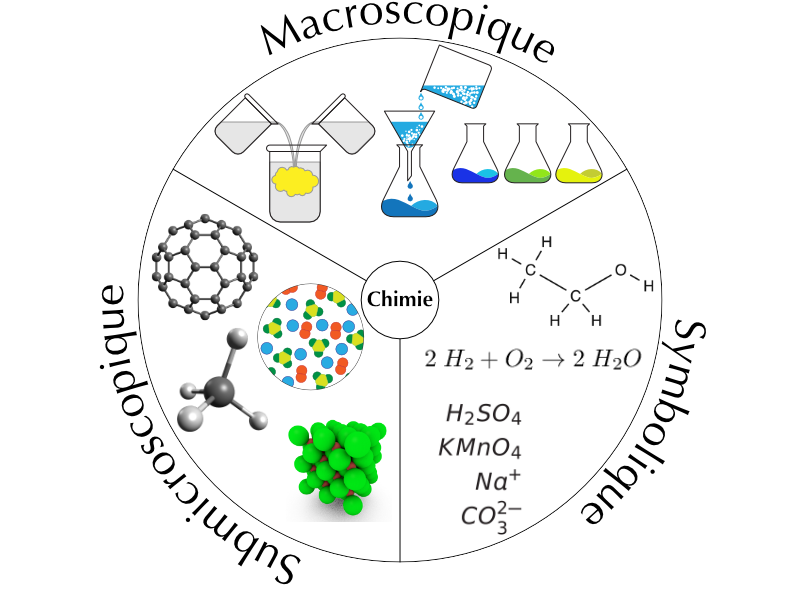
\includegraphics[width=0.5\linewidth]{images/Johnstone} 

}

\caption{Les trois niveaux de représentation de la chimie}\label{fig:Johnstone}
\end{figure}

Les propriétés macroscopiques sont régies par ce qu'il se passe au niveau submicroscopique.

\hypertarget{solide-liquide-et-gaz}{%
\section{Solide, liquide et gaz}\label{solide-liquide-et-gaz}}

La matière se trouve généralement sous trois formes physiques appelées états: solide, liquide et gaz.

\begin{longtable}[]{@{}cll@{}}
\toprule
\begin{minipage}[b]{0.05\columnwidth}\centering
\strut
\end{minipage} & \begin{minipage}[b]{0.38\columnwidth}\raggedright
\textbf{point de vue macroscopique}\strut
\end{minipage} & \begin{minipage}[b]{0.48\columnwidth}\raggedright
\textbf{point de vue submicroscopique}\strut
\end{minipage}\tabularnewline
\midrule
\endhead
\begin{minipage}[t]{0.05\columnwidth}\centering
\textbf{solide}\strut
\end{minipage} & \begin{minipage}[t]{0.38\columnwidth}\raggedright
Les solides ont un volume défini et une forme définie.\strut
\end{minipage} & \begin{minipage}[t]{0.48\columnwidth}\raggedright
Les particules sont peu mobiles et très proches.\strut
\end{minipage}\tabularnewline
\begin{minipage}[t]{0.05\columnwidth}\centering
\textbf{liquide}\strut
\end{minipage} & \begin{minipage}[t]{0.38\columnwidth}\raggedright
Les liquides ont un volume défini mais ils adoptent la forme de leur contenant.\strut
\end{minipage} & \begin{minipage}[t]{0.48\columnwidth}\raggedright
Les particules sont proches et se déplacent lentement aléatoirement.\strut
\end{minipage}\tabularnewline
\begin{minipage}[t]{0.05\columnwidth}\centering
\textbf{gaz}\strut
\end{minipage} & \begin{minipage}[t]{0.38\columnwidth}\raggedright
Les gaz occupent tout le volume et la forme de leur contenant.\strut
\end{minipage} & \begin{minipage}[t]{0.48\columnwidth}\raggedright
Les particules sont séparées par de grandes distances et se déplacent très rapidement aléatoirement.\strut
\end{minipage}\tabularnewline
\bottomrule
\end{longtable}

\begin{figure}

{\centering 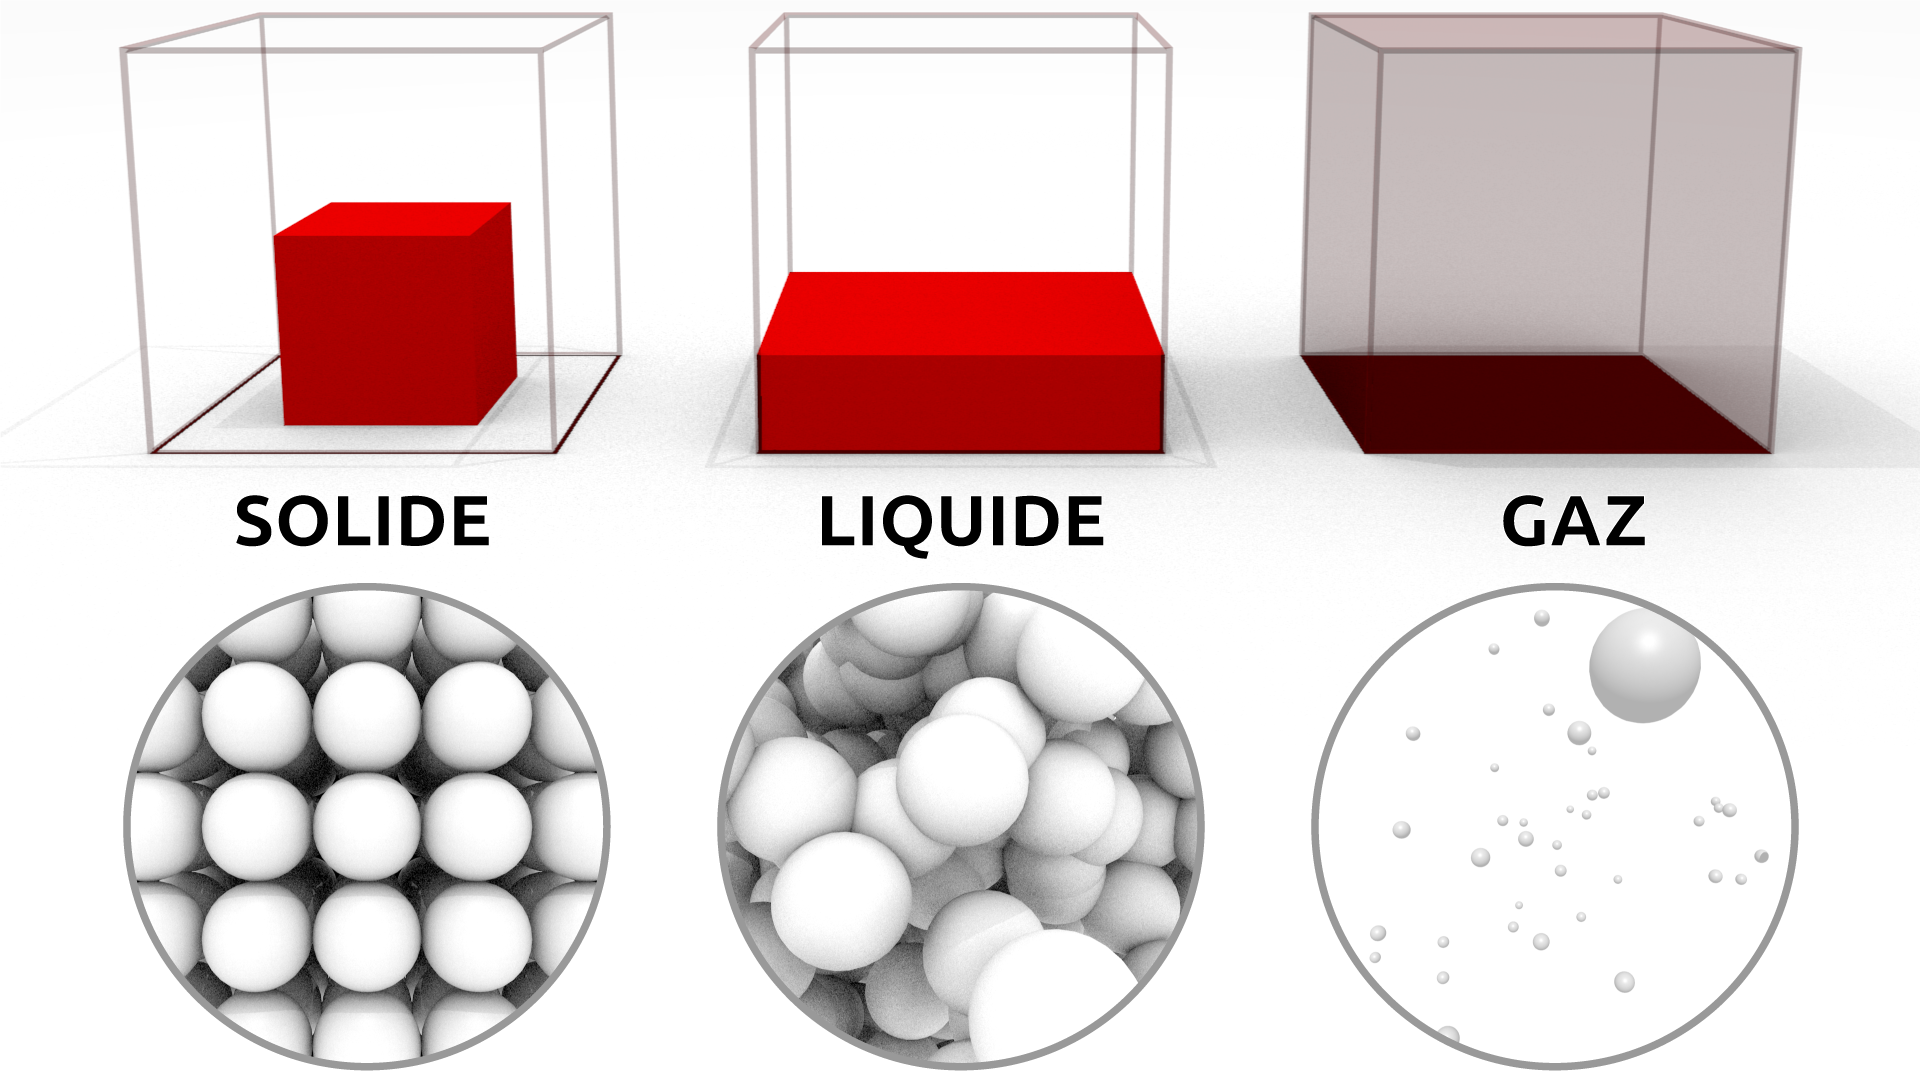
\includegraphics[width=0.5\linewidth]{images/solide-liquide-gaz} 

}

\caption{Les différents états de la matière du point de vue macroscopique et submicroscopique}\label{fig:solide-liquide-gaz}
\end{figure}

\hypertarget{mouvement-thermique-et-forces-intermoluxe9culaires}{%
\section{Mouvement thermique et forces intermoléculaires}\label{mouvement-thermique-et-forces-intermoluxe9culaires}}

La théorie cinétique de la matière nous indique que les particules qui composent la matière sont constamment en mouvement. Ce mouvement chaotique de particules est appelé \textbf{mouvement thermique}.

L'\textbf{énergie thermique} est l'énergie résultante du mouvement de ces particules. Elle est directement proportionnelle à la température de la substance. Cela signifie que plus la température augmente, plus les particules se déplacent rapidement et plus l'énergie qu'elles possèdent est élevée.

Il existe des forces d'attraction qui rassemblent les particules qui constituent la matière. Ces forces sont appelées les \textbf{forces intermoléculaires}. Ces forces sont d'origine électrostatique, elles sont dues à l'attraction entre des espèces chargées électriquement (positives et négatives).

\begin{itemize}
\tightlist
\item
  L'énergie thermique a tendance \textbf{à séparer} les particules qui forment la matière.
\item
  Les forces intermoléculaires ont tendance \textbf{à maintenir ensemble} les particules qui forment la matière.
\end{itemize}

Les trois états de la matière sont le résultat de l'\textbf{équilibre} entre les \textbf{forces intermoléculaires} et l'\textbf{énergie thermique}.

\begin{figure}

{\centering 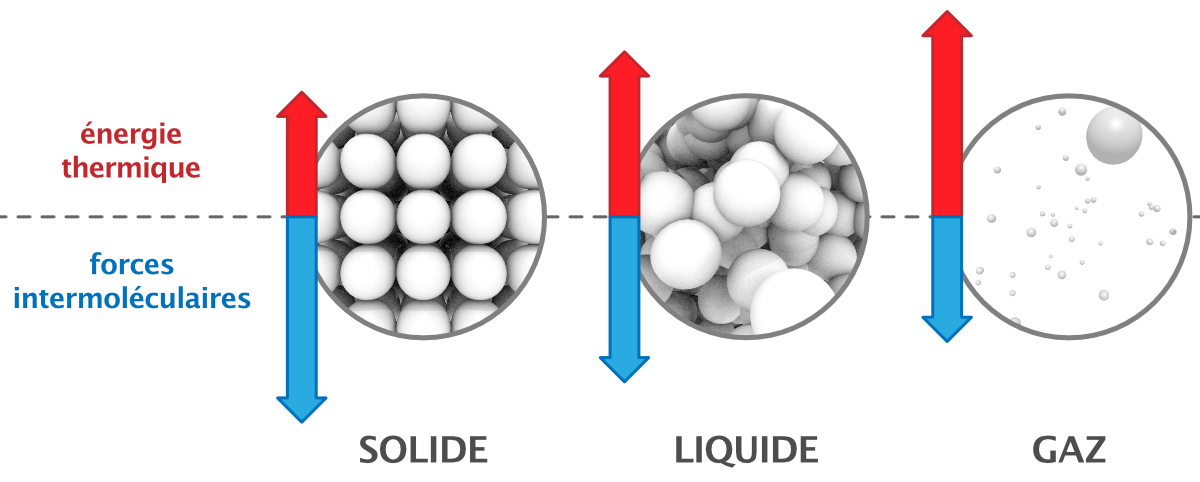
\includegraphics[width=0.67\linewidth]{images/mvt-thermique} 

}

\caption{Équilibre entre forces intermoléculaires et énergie thermique}\label{fig:mvt-thermique}
\end{figure}

Lorsque les forces intermoléculaires sont fortes et l'énergie thermique faible, la substance aura tendance à se trouver à l'état solide. Lorsque les forces intermoléculaires sont faibles et l'énergie thermique forte, la substance aura tendance à se trouver à l'état gazeux. L'état liquide résulte d'une équivalence entre forces intermoléculaires et énergie thermique.

\hypertarget{les-changements-duxe9tat}{%
\section{Les changements d'état}\label{les-changements-duxe9tat}}

En général, chaque état de la matière, solide, liquide ou gaz, peut se transformer en l'un des deux autres états. Ces transformations sont appelées \textbf{changements d'état}. Par exemple, l'eau peut subir deux changement d'état : elle fond à 0° C et bout à 100° C. Toutes les substances sont susceptibles de subir un changement d'état. Le fer fond à 1535° C et bout 2750° C.

On peut modifier l'état d'une substance en lui fournissant ou lui retirant de l'énergie thermique:

\textbf{Lorsque la température augmente}

\begin{itemize}
\tightlist
\item
  L'énergie thermique augmente.
\item
  Les particules se déplacent plus rapidement et se libèrent des forces d'attraction.
\end{itemize}

\textbf{Lorsque la température diminue}

\begin{itemize}
\tightlist
\item
  L'énergie thermique diminue.
\item
  Les particules se déplacent moins rapidement et les forces d'attraction les rassemblent.
\end{itemize}

\textbf{Les changements d'état sont des transformations physiques.} Lors d'un changement d'état une substance change la façon dont ses atomes ou molécules sont organisées sans changer les particules elles-mêmes.

\begin{itemize}
\tightlist
\item
  Le \textbf{point de fusion} est la température à laquelle une substance passe de l'état solide à l'état liquide.
\item
  Le \textbf{point d'ébullition} est la température à laquelle une substance passe de l'état liquide à l'état gazeux.
\end{itemize}

L'\textbf{évaporation} est la transformation d'un liquide en vapeur sans ébullition. Il peut y avoir vaporisation sans ébullition de la matière.

\newpage

\begin{figure}

{\centering 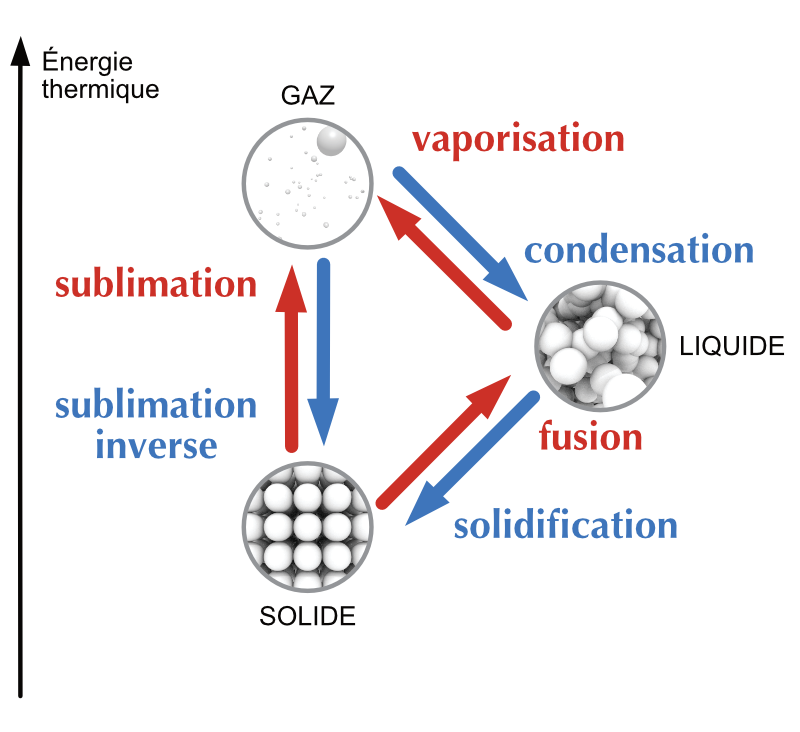
\includegraphics[width=0.45\linewidth]{images/chgt-etats} 

}

\caption{Les noms des changements d'état}\label{fig:chgt-etats}
\end{figure}

\begin{Exercise}

\begin{enumerate}
\def\labelenumi{\arabic{enumi}.}
\tightlist
\item
  Lequel(s) des énoncés suivants décrit ce qui se passe lorsque des particules d'eau gèlent ?

  \begin{enumerate}
  \def\labelenumii{\alph{enumii}.}
  \tightlist
  \item
    Elles gagnent de l'énergie et de l'espace pour se déplacer.
  \item
    Elles gagnent de l'énergie et se décomposent en atomes d'hydrogène et d'oxygène.
  \item
    Elles perdent de l'énergie et s'échappent dans l'atmosphère.
  \item
    Elles perdent de l'énergie et de l'espace pour se déplacer.
  \end{enumerate}
\item
  Lequel(s) des énoncés suivants décrit le mieux le comportement des particules dans un gaz ?

  \begin{enumerate}
  \def\labelenumii{\alph{enumii}.}
  \tightlist
  \item
    Éloignées et se déplaçant lentement.
  \item
    Rapprochées et immobiles.
  \item
    Rapprochées et en vibration.
  \item
    Très éloignés et se déplaçant très rapidement.
  \end{enumerate}
\item
  Lequel(s) des énoncés suivants est vrai pour gaz qui condense ?

  \begin{enumerate}
  \def\labelenumii{\alph{enumii}.}
  \tightlist
  \item
    Le gaz libère de l'énergie thermique.
  \item
    La température du gaz augmente.
  \item
    Les particules de gaz perdent de leur liberté de mouvement.
  \item
    Les particules de gaz diminuent en taille.
  \end{enumerate}
\item
  Lequel(s) des énoncés suivants est vrai pour un liquide passant à l'état gazeux ?

  \begin{enumerate}
  \def\labelenumii{\alph{enumii}.}
  \tightlist
  \item
    La température du liquide reste constante.
  \item
    Les particules de liquide gagnent en liberté de mouvement.
  \item
    Les particules de liquide augmentent en taille.
  \item
    Le liquide libère de l'énergie thermique.
  \end{enumerate}
\item
  Lequel(s) des énoncés suivants est vrai pour un liquide passant à l'état solide ?

  \begin{enumerate}
  \def\labelenumii{\alph{enumii}.}
  \tightlist
  \item
    Le liquide libère de l'énergie thermique.
  \item
    Les particules de liquide diminuent en taille.
  \item
    La température reste constante.
  \item
    Les particules de liquide augmentent leur liberté de mouvement.
  \end{enumerate}
\end{enumerate}


\end{Exercise}

\begin{Answer}

\begin{enumerate}
\def\labelenumi{\arabic{enumi}.}
\tightlist
\item
  Lequel(s) des énoncés suivants décrit ce qui se passe lorsque des particules d'eau gèlent?

  \begin{enumerate}
  \def\labelenumii{\alph{enumii}.}
  \setcounter{enumii}{3}
  \tightlist
  \item
    \textbf{Elles perdent de l'énergie et de l'espace pour se déplacer.}
  \end{enumerate}
\item
  Lequel(s) des énoncés suivants décrit le mieux le comportement des particules dans un gaz?

  \begin{enumerate}
  \def\labelenumii{\alph{enumii}.}
  \setcounter{enumii}{3}
  \tightlist
  \item
    \textbf{Très éloignés et se déplaçant très rapidement.}
  \end{enumerate}
\item
  Lequel(s) des énoncés suivants est vrai pour gaz qui condense?

  \begin{enumerate}
  \def\labelenumii{\alph{enumii}.}
  \tightlist
  \item
    \textbf{Le gaz libère de l'énergie thermique.}
  \item
    \textbf{Les particules de gaz perdent de leur liberté de mouvement.}
  \end{enumerate}
\item
  Lequel(s) des énoncés suivants est vrai pour un liquide passant à l'état gazeux?

  \begin{enumerate}
  \def\labelenumii{\alph{enumii}.}
  \tightlist
  \item
    \textbf{La température du liquide reste constante.}
  \item
    \textbf{Les particules de liquide gagnent en liberté de mouvement.}
  \end{enumerate}
\item
  Lequel(s) des énoncés suivants est vrai pour un liquide passant à l'état solide?

  \begin{enumerate}
  \def\labelenumii{\alph{enumii}.}
  \tightlist
  \item
    \textbf{Le liquide libère de l'énergie thermique.}
  \item
    \textbf{La température reste constante.}
  \end{enumerate}
\end{enumerate}


\end{Answer}

\begin{Exercise}

Un coton imbibé d'éther mis en contact sur la peau provoque une sensation de froid. On sait, par ailleurs, que l'éther passe facilement de l'état liquide à l'état gazeux.

\begin{enumerate}
\def\labelenumi{\arabic{enumi}.}
\item
  Quel nom donne-t-on à ce changement d'état ?
  ~
\item
  Quelle conclusion (scientifique) peut-on mettre en relation avec la sensation de froid mentionné ?
  ~
\end{enumerate}


\end{Exercise}

\begin{Answer}

\begin{enumerate}
\def\labelenumi{\arabic{enumi}.}
\tightlist
\item
  Quel nom donne-t-on à ce changement d'état ?
  \textbf{La vaporisation}
\item
  Quelle conclusion (scientifique) peut-on mettre en relation avec la sensation de froid mentionné ?
  \textbf{L'éther absorbe la chaleur du corps pour vaporiser, d'où la sensation de froid.}
\end{enumerate}


\end{Answer}

\hypertarget{les-courbes-de-changement-duxe9tat}{%
\section{Les courbes de changement d'état}\label{les-courbes-de-changement-duxe9tat}}

\begin{figure}

{\centering 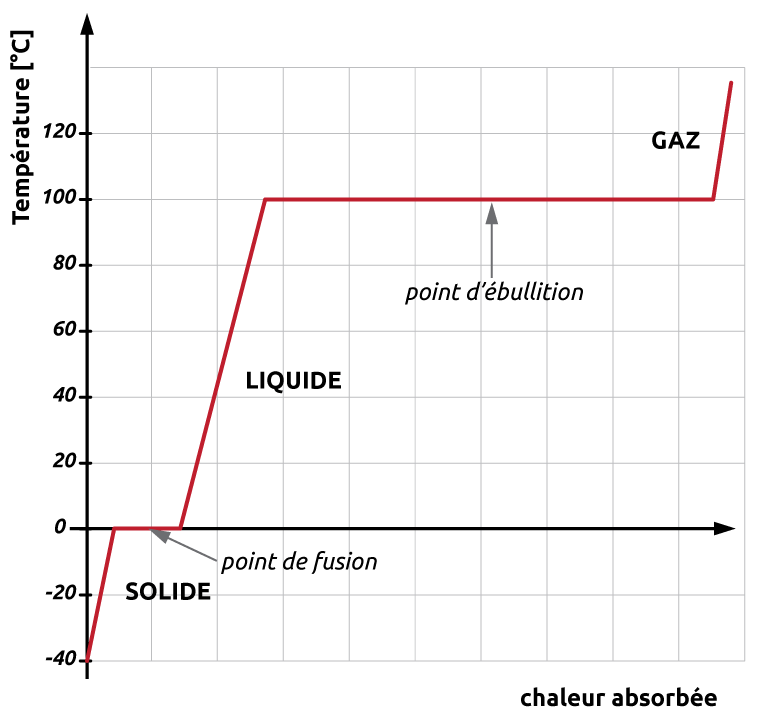
\includegraphics[width=0.4\linewidth]{images/courbe-chgt-etat} 

}

\caption{Courbe de chauffage de l'eau}\label{fig:courbe-chgt-etat}
\end{figure}

Imaginons que l'on chauffe un bloc de glace en partant d'une température de -40° C. On place un thermomètre dans notre expérimentation et on note la température.

\begin{itemize}
\tightlist
\item
  En chauffant, on apporte de l'énergie thermique au système. La glace se réchauffe et sa température augmente.
\item
  Une fois que la glace atteint 0° C, \textbf{la température cesse d'augmenter} et la glace commence à fondre pour former de l'eau liquide.
\item
  En continuant de chauffer, plus de glace se transforme en eau, mais la température reste la même.
\item
  Une fois que la glace a complètement fondu, la chaleur apportée chauffe l'eau liquide.
  La température recommence à augmenter.
\item
  Une fois que l'eau liquide atteint 100° C, \textbf{la température cesse d'augmenter} et l'eau commence à vaporiser pour former de la vapeur d'eau.
\item
  En continuant de chauffer, plus d'eau liquide se transforme en vapeur d'eau, mais la température reste la même.
\item
  Une fois que l'eau s'est complètement vaporisée, la chaleur apportée chauffe la vapeur d'eau.
  La température recommence à augmenter.
\end{itemize}

Un changement de température et un changement d'état ne se produisent pas en même temps. Quand une substance absorbe ou libère de l'énergie, soit c'est la température qui change, soit c'est son état. En d'autres termes, \textbf{la température d'une substance ne change pas au cours d'un changement d'état.}

En effectuant la même expérience, mais en partant de vapeur d'eau chaude et en diminuant la température, la courbe serait inversée et aurait la même allure.

\hypertarget{les-diagrammes-de-phases}{%
\section{Les diagrammes de phases}\label{les-diagrammes-de-phases}}

Nous avons vu qu'il est possible de liquéfier un gaz à pression ambiante en le refroidissant. Pourtant, cela ne suffit pas toujours. Par exemple, on sait qu'à pression atmosphérique, le dioxyde de carbone CO\textsubscript{2} passe directement de la phase gazeuse à la phase solide (sublimation inverse). Ainsi, pour obtenir du CO\textsubscript{2} liquide, il est nécessaire d'augmenter la pression.

Ce genre d'informations est résumé sur un \textbf{diagramme de phases} qui donne les conditions (pression et température) d'existence des différentes phases d'une substance donnée.

\begin{figure}

{\centering 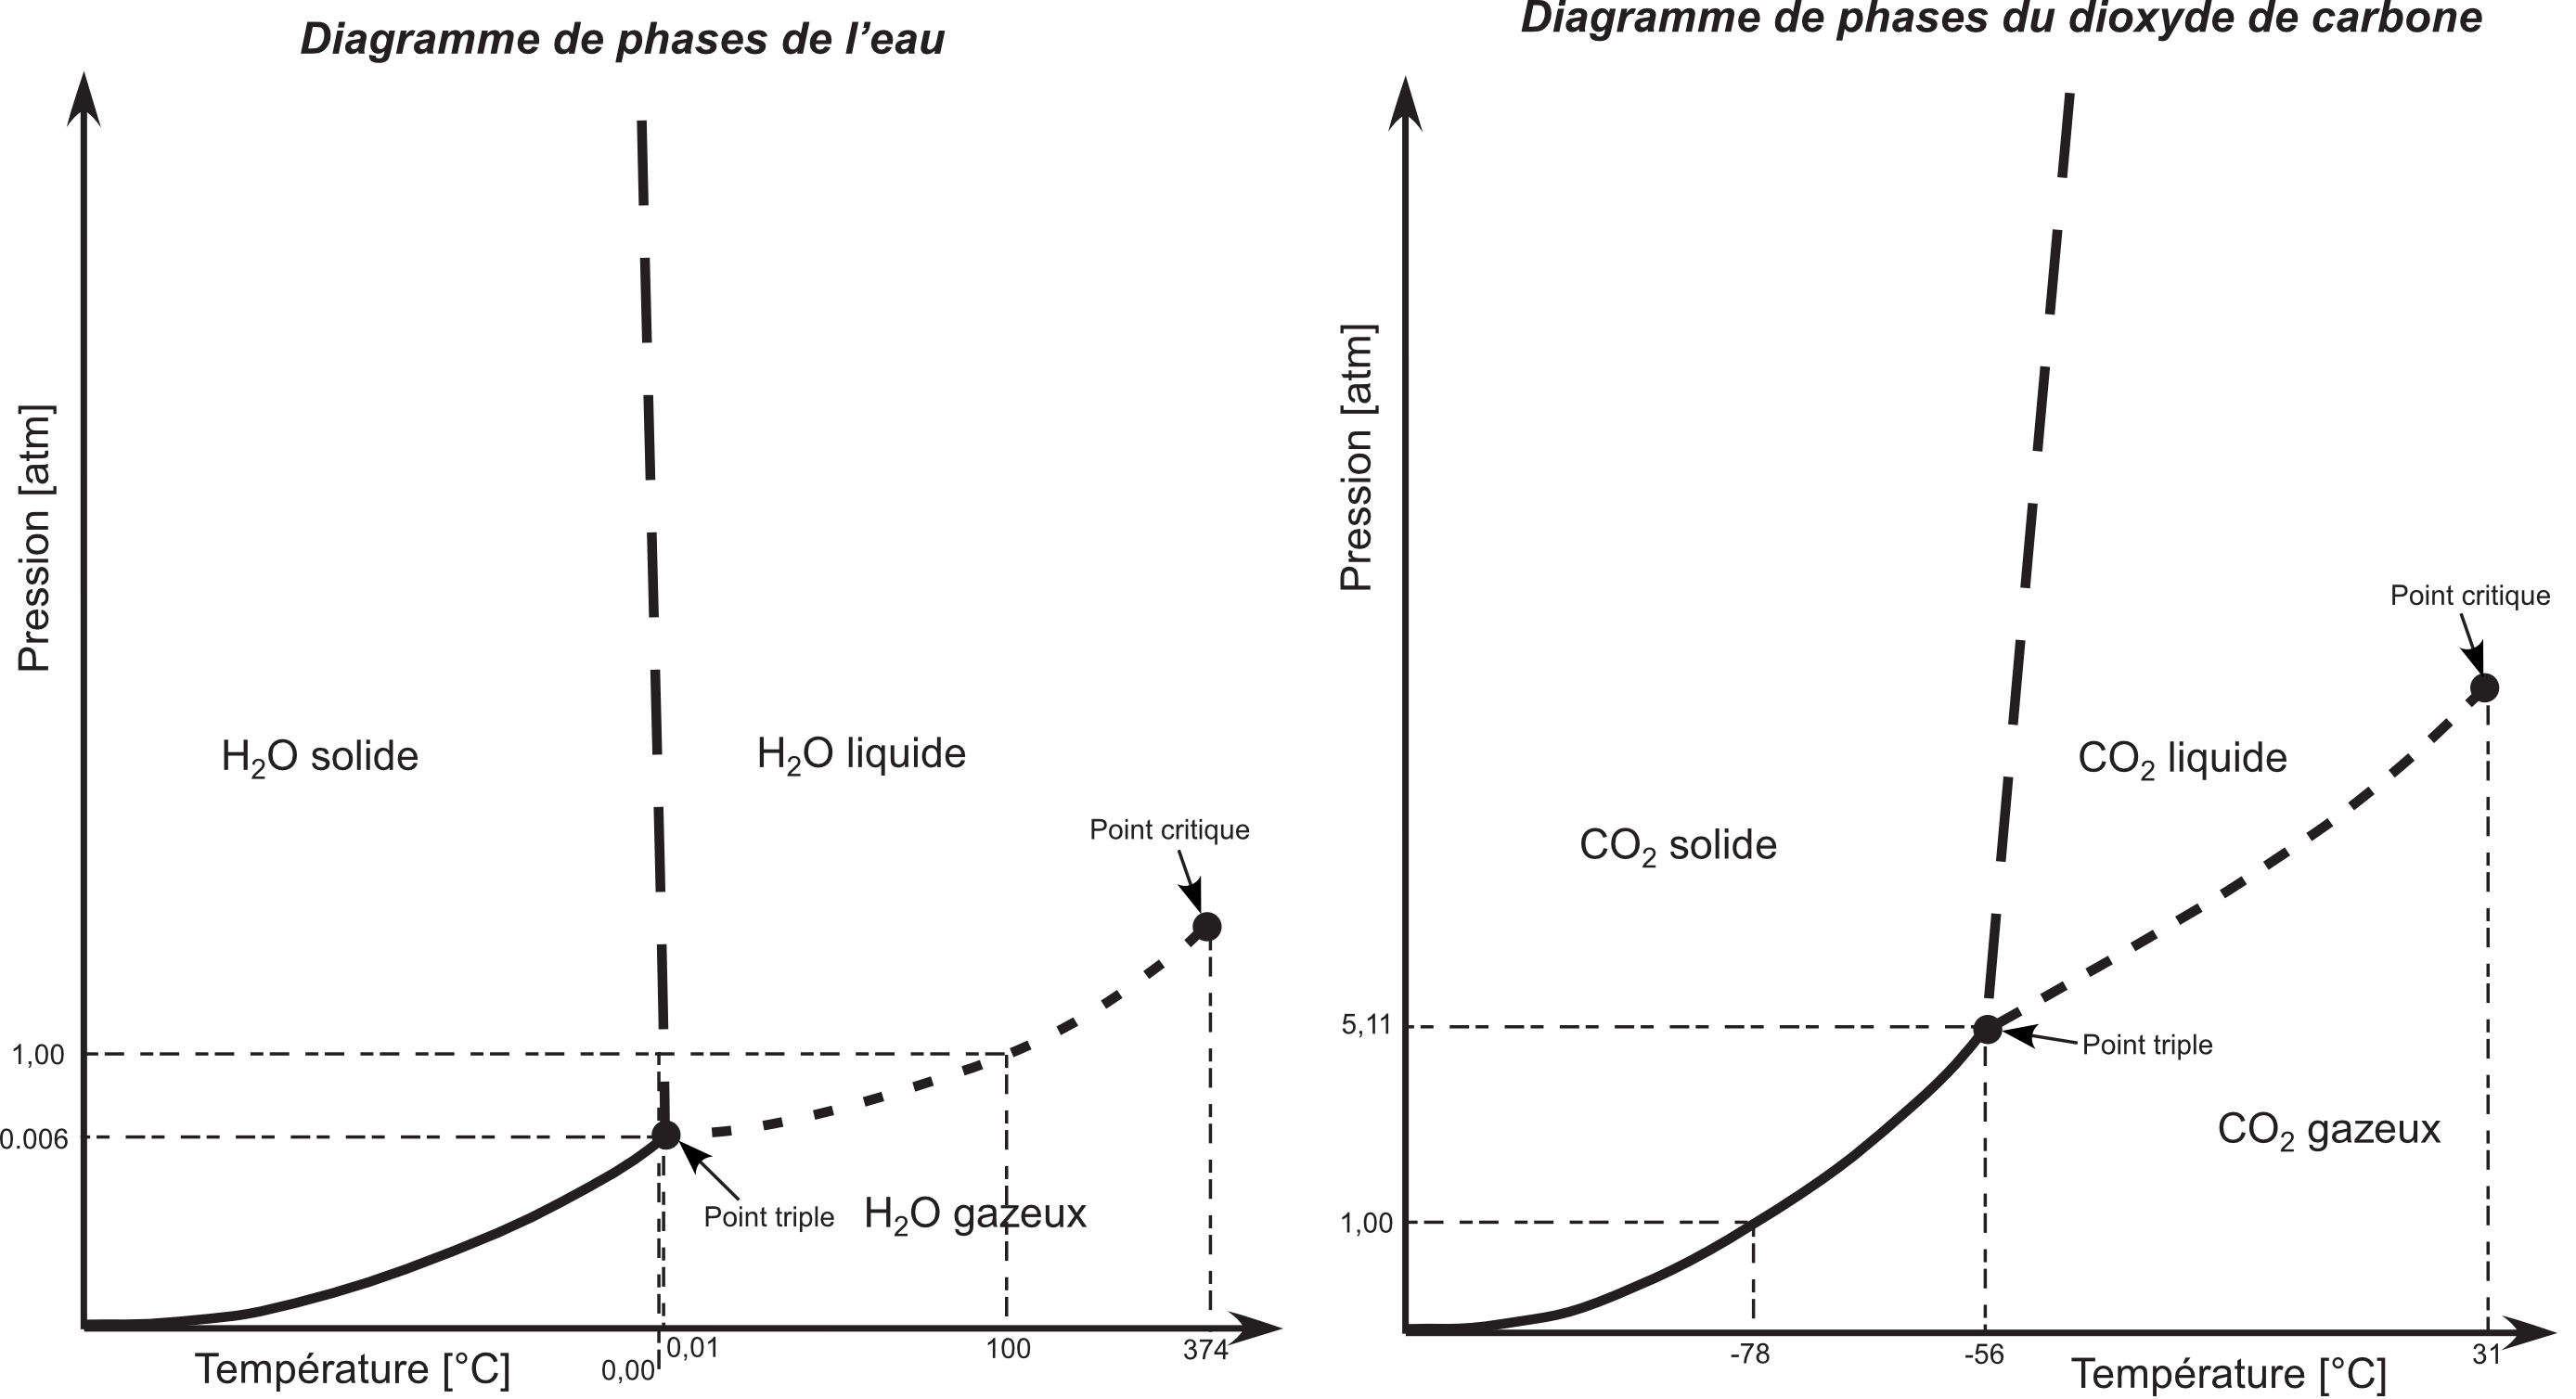
\includegraphics[width=1\linewidth]{images/diagramme-phases-eau-CO2} 

}

\caption{Diagramme de phases de l'eau et du CO~2~ (Les échelles ne sont pas régulières)}\label{fig:diagramme-phases-eau-CO2}
\end{figure}

\begin{Exercise}

\begin{enumerate}
\def\labelenumi{\arabic{enumi}.}
\tightlist
\item
  Quelle est la pression minimale pour que le CO\textsubscript{2} liquide puisse exister ?\\
  \vspace{\stretch{1}}
\item
  Quelle doit alors être la température ?\\
  \vspace{\stretch{1}}
\item
  Que représente le point triple ?\\
  \vspace{\stretch{1}}
\item
  Que se passe-t-il si on prend de l'eau à 0.005 {[}atm{]} et --200° C et qu'on augmente la température jusqu'à 300° C ?\\
  \vspace{\stretch{1}}
\item
  Même question pour le CO\textsubscript{2}.\\
  \vspace{\stretch{1}}
\end{enumerate}


\end{Exercise}

\begin{Answer}

\begin{enumerate}
\def\labelenumi{\arabic{enumi}.}
\tightlist
\item
  5.11 {[}atm{]}
\item
  -56° C
\item
  Les conditions dans lesquelles trois phases différentes peuvent coexister.
\item
  L'eau ne sera jamais liquide.
\item
  Le CO\textsubscript{2} ne sera jamais liquide.
\end{enumerate}


\end{Answer}

\newpage

\hypertarget{luxe9tat-liquide}{%
\section{L'état liquide}\label{luxe9tat-liquide}}

Au niveau submicroscopique, les particules qui forment les liquides suivent des mouvements aléatoires constants. Elles peuvent être ordonnées sur de courtes portions, mais cela ne dure pas très longtemps.

\begin{figure}

{\centering 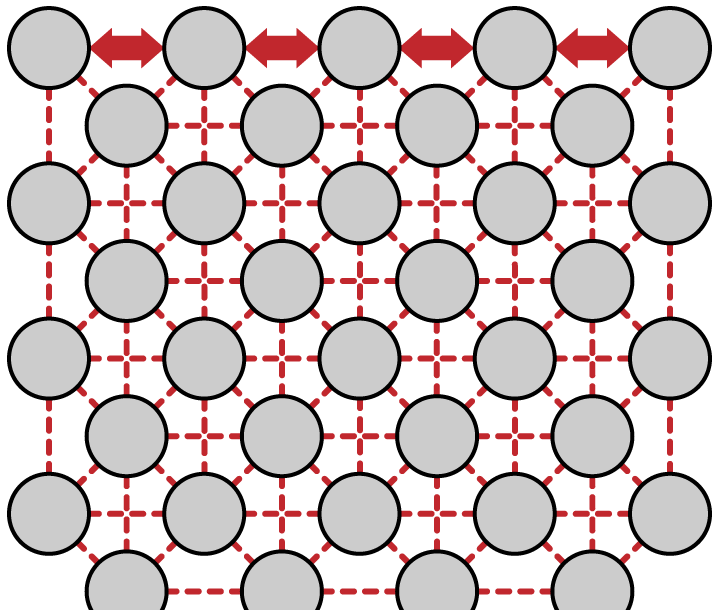
\includegraphics[width=0.33\linewidth]{images/tension-surface} 

}

\caption{Tension superficielle}\label{fig:tension-surface}
\end{figure}

Les forces intermoléculaires ont des effets différents sur une particule à la surface que sur une particule dans le corps du liquide.

\begin{itemize}
\tightlist
\item
  Une particule à l'intérieur du liquide est attirée par d'autres particules dans toutes les directions.
\item
  Une particule en surface n'est attirée dans le corps du liquide que par les côtés et en dessous, mais pas au-dessus.
\end{itemize}

Cette attraction inégale fait que le liquide a un volume propre et ne se disperse pas. Ce phénomène est appelé \textbf{tension superficielle}.

La \textbf{viscosité} est la résistance à l'écoulement d'un liquide. Elle dépend des forces intermoléculaires et de la température. Les liquides ayant des forces intermoléculaires fortes ont tendance à avoir une viscosité élevée.

La \textbf{capillarité} est la tendance qu'a un liquide à monter le long d'un tube étroit. Elle est causée par la compétition entre les forces intermoléculaires dans le liquide et les forces d'attraction entre le liquide et la paroi du tube.

\begin{figure}

{\centering 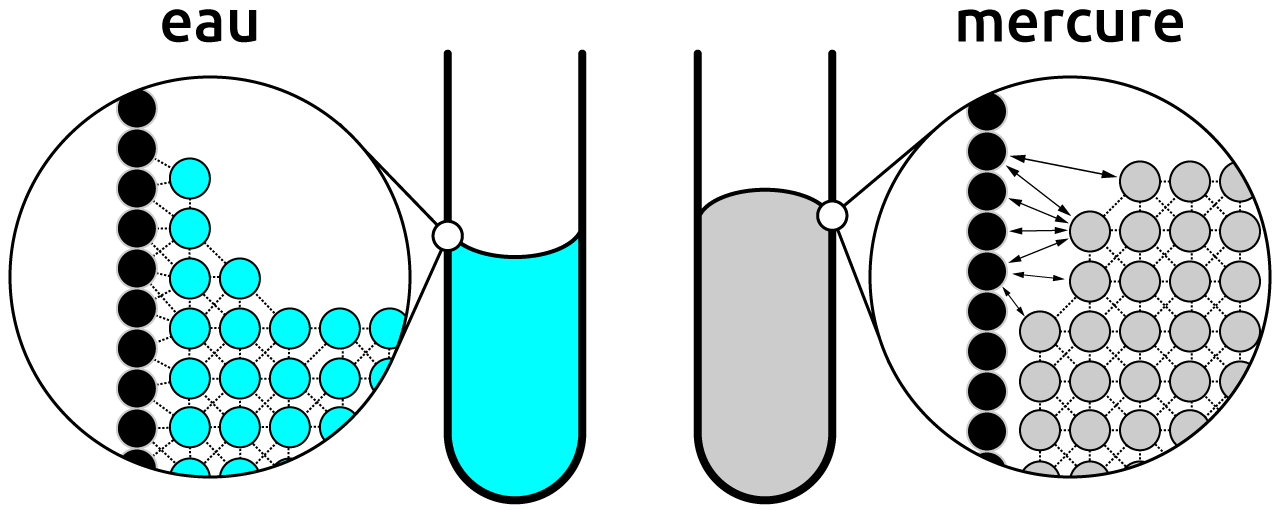
\includegraphics[width=0.67\linewidth]{images/capillarity} 

}

\caption{La capillarité}\label{fig:capillarity}
\end{figure}

\newpage

\hypertarget{luxe9tat-solide}{%
\section{L'état solide}\label{luxe9tat-solide}}

Au niveau submicroscopique, les solides peuvent être de deux types - amorphe ou cristallin.

\begin{figure}

{\centering 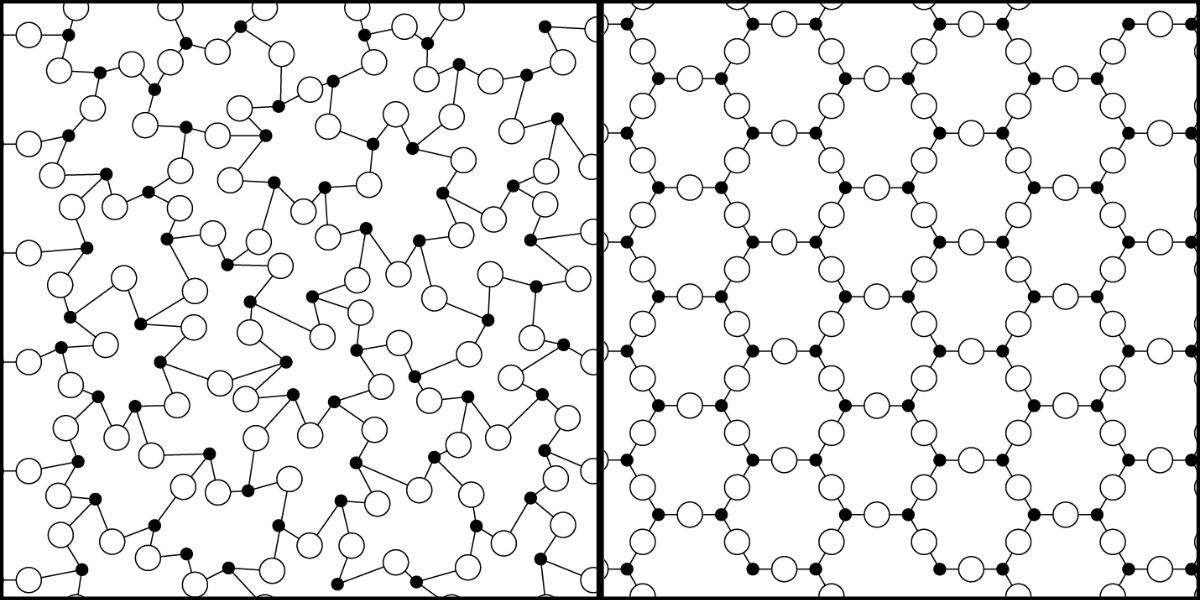
\includegraphics[width=0.45\linewidth]{images/amorphous} 

}

\caption{Solide amorphe (Verre) - Solide cristallin (Quartz)}\label{fig:amorphous}
\end{figure}

\hypertarget{les-solides-amorphes}{%
\subsection{Les solides amorphes}\label{les-solides-amorphes}}

Les particules formant les solides amorphes ne sont pas ordonnées sur de grandes portions de l'espace. Leur structure est irrégulière et ressemble plus à la structure d'un liquide qui serait figé.

Les solides amorphes n'ont pas un point de fusion distinct. Ils deviennent simplement plus souple lorsque la température augmente. Le verre, le caoutchouc ou le beurre sont des exemples de solides amorphes.

\hypertarget{les-solides-cristallins}{%
\subsection{Les solides cristallins}\label{les-solides-cristallins}}

Les particules formant les solides cristallins sont assemblées les unes par rapport aux autres de façon régulière sur de vastes portions de l'espace. Cette structure tridimensionnelle est appelée \textbf{réseau cristallin}.

Une \textbf{maille} est un volume de cristal, qui, lorsqu'il est répété dans les trois dimensions de l'espace, permet d'obtenir le cristal tout entier.

\begin{figure}

{\centering 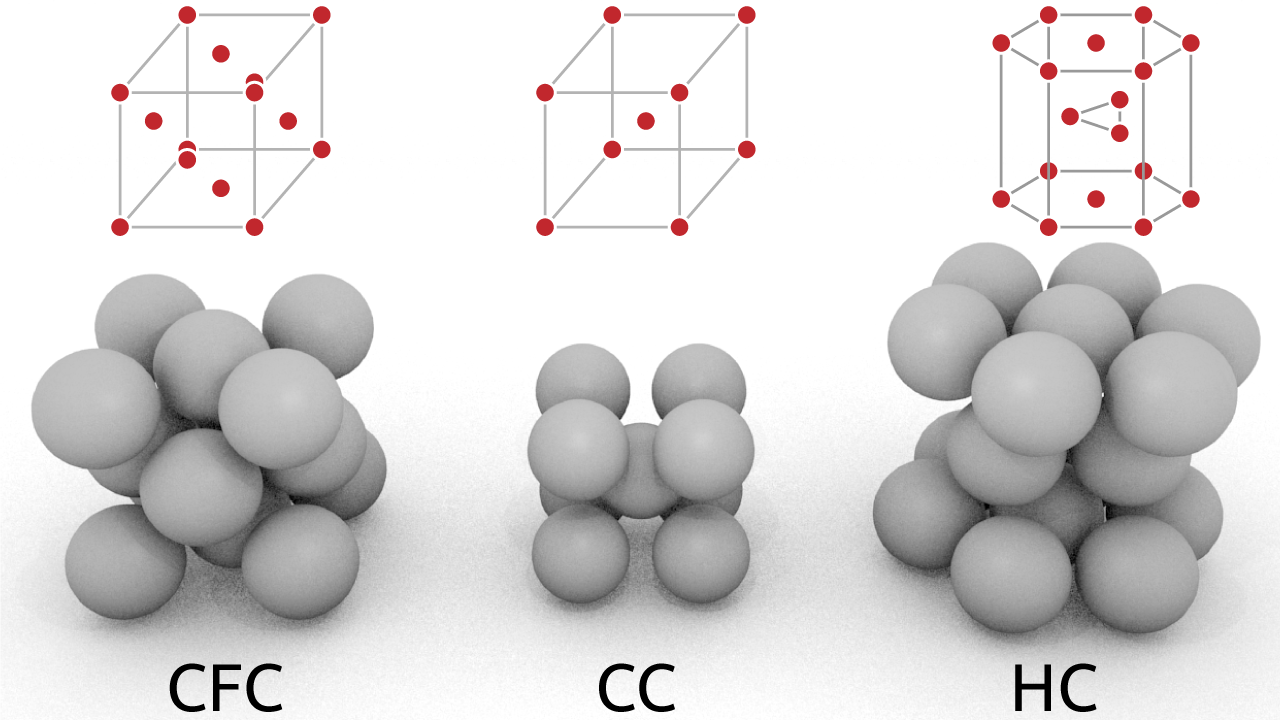
\includegraphics[width=0.67\linewidth]{images/metaux} 

}

\caption{3 mailles de réseaux cristallins classiques (CFC: cubique à face centrées, CC: cubique centré, HC: hexagonal compact)}\label{fig:metaux}
\end{figure}

\hypertarget{allotropes}{%
\subsection{Allotropes}\label{allotropes}}

L'\textbf{allotropie} est la propriété qu'ont certains corps à former des cristaux de différentes formes, appelés \textbf{allotropes} de cette substance. Par exemple, le diamant, le graphite et les fullerènes sont des formes allotropiques du carbone: formés du même élément mais dont la structure cristalline est différente.

\begin{figure}

{\centering 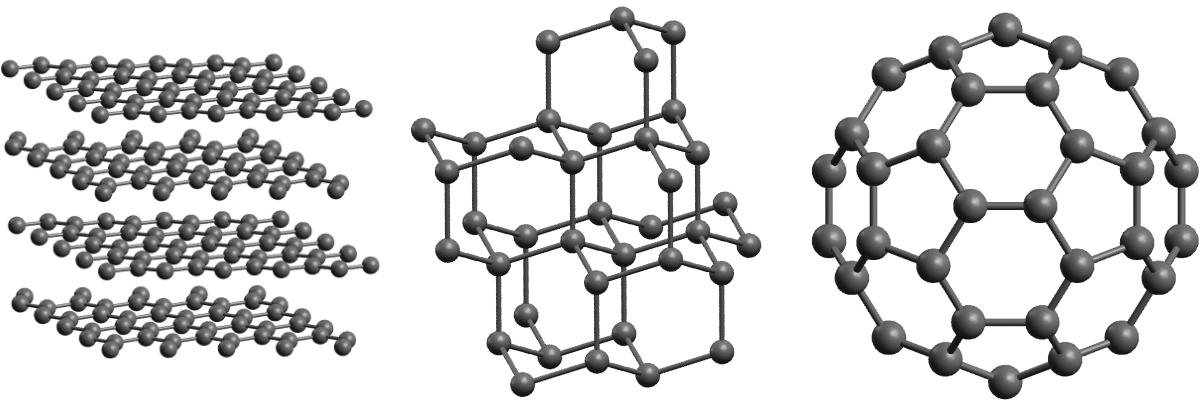
\includegraphics[width=0.45\linewidth]{images/allotropes} 

}

\caption{Trois formes allotropiques du carbone (graphite, diamant, fullerène)}\label{fig:allotropes}
\end{figure}

\hypertarget{exercices-suppluxe9mentaires-1}{%
\section{Exercices supplémentaires}\label{exercices-suppluxe9mentaires-1}}

\begin{Exercise}

\begin{enumerate}
\def\labelenumi{\arabic{enumi}.}
\tightlist
\item
  Pourquoi en montagne le point d'ébullition de l'eau diminue-t-il par rapport à celui observé au niveau de la mer ?\\
  \vspace{\stretch{1}}
\item
  Expliquez ce que sont les bulles qui apparaissent lorsque l'eau bout.\\
  \vspace{\stretch{1}}
\item
  Qu'est-ce que la condensation ? Citez un exemple de la vie pratique où vous pouvez observer de la condensation.\\
  \vspace{\stretch{1}}
\item
  Pourquoi met-on du sel sur les routes en hiver ?\\
  \vspace{\stretch{1}}
\end{enumerate}


\end{Exercise}

\begin{Answer}

\begin{enumerate}
\def\labelenumi{\arabic{enumi}.}
\tightlist
\item
  En montagne la pression atmosphérique est plus basse ce qui abaisse le point d'ébullition de l'eau.\\
\item
  Les bulles, visibles à l'intérieur du liquide, sont des bulles de vapeur d'eau.\\
\item
  Passage de l'eau de l'état gazeux à l'état liquide. Rosée du matin, buée sur les vitres, gouttelettes d'eau sur une boisson sortie du réfrigérateur, \ldots{}\\
\item
  Les impuretés abaissent le point de fusion d'une substance. Le sel abaisse le point de fusion de l'eau, ainsi elle gèlera à une température inférieure à 0° C.
\end{enumerate}

\newpage


\end{Answer}

\begin{Exercise}
Complétez le tableau suivant en décrivant le changement d'état. Le tableau a été partiellement complété pour vous aider.

\end{Exercise}

\begin{longtable}[]{@{}lcc@{}}
\toprule
& Changement d'état & libère ou absorbe de la chaleur\tabularnewline
\midrule
\endhead
condensation & & libère\tabularnewline
sublimation & &\tabularnewline
vaporisation & liquide \(\rightarrow\) gaz &\tabularnewline
fusion & & absorbe\tabularnewline
solidification & &\tabularnewline
sublimation inverse & &\tabularnewline
\bottomrule
\end{longtable}

\begin{Answer}
condensation / gaz \(\rightarrow\) liquide / libère

sublimation / solide \(\rightarrow\) gaz / absorbe

vaporisation / liquide \(\rightarrow\) gaz / absorbe

fusion / solide \(\rightarrow\) liquide / absorbe

solidification / liquide \(\rightarrow\) solide / libère

sublimation inverse / gaz \(\rightarrow\) solide / libère

\end{Answer}

\begin{Exercise}
Connaissant les points de fusion et d'ébullition des substances suivantes, donnez l'état physique de la substance à température ambiante (25° C).

\end{Exercise}

\begin{longtable}[]{@{}lccc@{}}
\toprule
substance & point de fusion & point d'ébullition & état physique à 25° C\tabularnewline
\midrule
\endhead
eau & 0° C & 100° C &\tabularnewline
méthane & -182° C & -162° C &\tabularnewline
fer & 1535° C & 2750° C &\tabularnewline
mercure & -39° C & 357° C &\tabularnewline
oxygène & -218° C & -183° C &\tabularnewline
or & 1063° C & 2856° C &\tabularnewline
\bottomrule
\end{longtable}

\begin{Answer}
eau : liquide

méthane : gaz

fer : solide

mercure : liquide

oxygène : gaz

or : solide

\end{Answer}

\newpage

\begin{Exercise}

On refroidit un liquide, tout en mesurant régulièrement sa température. Voici les résultats obtenu :

\begin{itemize}
\tightlist
\item
  Temps (en min) : 0, 1, 2, 3, 4, 5, 6, 7, 8, 9
\item
  Température (en °C) : 20, 15, 10, 5, 5, 5, 5, 5, 0, -5
\end{itemize}

\begin{enumerate}
\def\labelenumi{\arabic{enumi}.}
\tightlist
\item
  Tracez le graphique représentant l'évolution de la température du liquide en fonction du temps lors de son refroidissement.
\end{enumerate}

\begin{center}
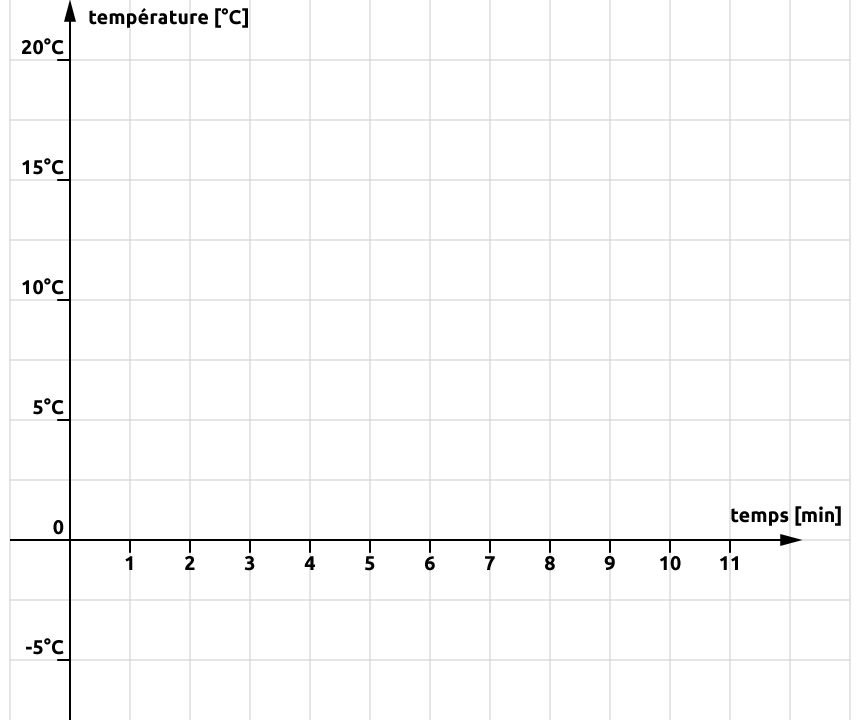
\includegraphics[width=0.75\textwidth,height=\textheight]{images/graph-cyclohexane.png}

\end{center}

\begin{enumerate}
\def\labelenumi{\arabic{enumi}.}
\setcounter{enumi}{1}
\tightlist
\item
  Quel changement d'état à lieu ici ?\\
  \vspace{\stretch{1}}
\item
  Délimitez, sur le graphique, le début et la fin du changement d'état et indiquez les états physiques observés.
\item
  Ce liquide est-il de l'eau? (Justifiez)
  \vspace{\stretch{1}}
\item
  En vous aidant des informations ci-dessous, déterminez quelle est la substance refroidie.\\
  Température de solidification\\
\end{enumerate}

\begin{itemize}
\tightlist
\item
  Acide lactique : 17° C
\item
  Anéthole : 20° C
\item
  Cyclohexane : 5° C
  \vspace{\stretch{1}}
\end{itemize}

\begin{enumerate}
\def\labelenumi{\arabic{enumi}.}
\setcounter{enumi}{5}
\tightlist
\item
  Quelle est la température de fusion du cyclohexane ? Justifiez.\\
  \vspace{\stretch{1}}
\end{enumerate}


\end{Exercise}

\begin{Answer}

\begin{center}
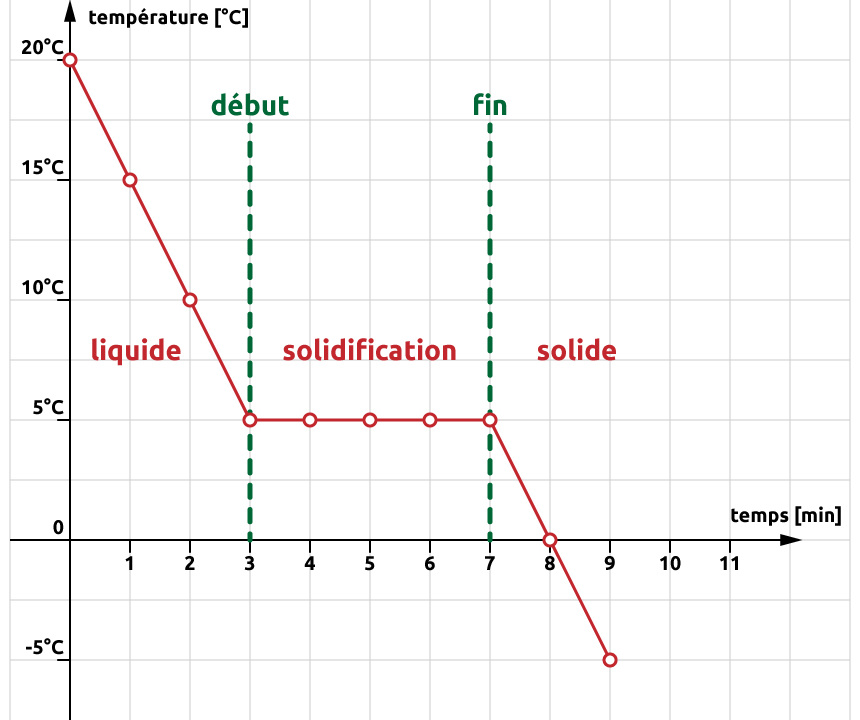
\includegraphics[width=0.67\textwidth,height=\textheight]{images/graph-cyclohexane-corr.png}

\end{center}

\begin{enumerate}
\def\labelenumi{\arabic{enumi}.}
\setcounter{enumi}{1}
\tightlist
\item
  La solidification
\item
  Non, car l'eau solidifie à 0° C.
\item
  Le cyclohexane, température de solidification = 5° C.
\item
  5° C, température de fusion = température de solidification.
\end{enumerate}


\end{Answer}

\newpage

\section{Solutions des exercices} \shipoutAnswer

\hypertarget{muxe9langes-et-corps-purs}{%
\chapter{Mélanges et corps purs}\label{muxe9langes-et-corps-purs}}

\begin{objectives}

\begin{itemize}
\tightlist
\item
  Identifier les corps simples et composés.
\item
  Identifier les mélanges homogènes et hétérogènes.
\item
  Savoir choisir la méthode de séparation adaptée à un mélange.
\end{itemize}


\end{objectives}

La première question que se pose un chimiste à propos d'un échantillon de matière inconnu est de savoir s'il s'agit d'une substance pure ou d'un mélange. Chaque échantillon de matière est l'un ou l'autre.

Lorsque nous parlons d'une substance pure, nous parlons de quelque chose qui ne contient qu'un seul type de matière. Il peut s'agir d'un seul élément ou d'un seul composé, mais chaque échantillon de cette substance que vous examinez doit contenir exactement la ``même chose'' et avoir les mêmes propriétés. Si nous prenons deux ou plusieurs substances pures et que nous les mélangeons, nous parlerons naturellement d'un mélange.

Selon la nature des particules qui la compose, la matière peut être classée en trois types : les \textbf{corps purs simples}, les \textbf{corps purs composés} et les \textbf{mélanges}.

\hypertarget{corps-pur-simple}{%
\section{Corps pur simple}\label{corps-pur-simple}}

\begin{tcolorbox}
\textbf{Corps pur simple}\\
Un corps pur simple est constitué d'atomes d'un seul élément.

\end{tcolorbox}

Un corps pur simple est le type le plus simple de composition de la matière. Il s'agit d'un \textbf{assemblage d'atomes d'un seul élément} avec des propriétés physiques et chimiques uniques.

Chaque élément a un nom comme le silicium, l'oxygène ou le cuivre. Un morceau de silicium ne contient que des atomes de silicium et un morceau de cuivre ne contient que des atomes de cuivre. Les \textbf{propriétés macroscopiques} d'un morceau de silicium, comme la couleur ou la densité, sont différentes de celles d'un morceau de cuivre, car les \textbf{propriétés submicroscopiques} des atomes de silicium sont différentes de celles des atomes de cuivre.

\hypertarget{corps-pur-composuxe9}{%
\section{Corps pur composé}\label{corps-pur-composuxe9}}

\begin{tcolorbox}
\textbf{Corps pur composé}\\
Un corps pur composé est constitué de deux ou plusieurs éléments différents qui sont liés ensemble chimiquement.

\end{tcolorbox}

Les particules qui forment un corps pur composé sont des atomes qui sont liés ensemble suite à une réaction chimique. Ces atomes ne sont pas simplement mélangés ensemble.

Par exemple, l'eau (H\textsubscript{2}O) est un corps pur composé constitué de deux éléments, l'hydrogène et l'oxygène. Ces éléments sont combinés d'une manière très spécifique, deux atomes d'hydrogène pour un atome d'oxygène (d'où H\textsubscript{2}O). Plusieurs composés contiennent de l'hydrogène et de l'oxygène, mais un seul a ce rapport spécifique de 2 pour 1, c'est l'eau.

Un corps pur composé a des propriétés physiques et chimiques différentes de celles des éléments qui le composent.

\begin{figure}

{\centering 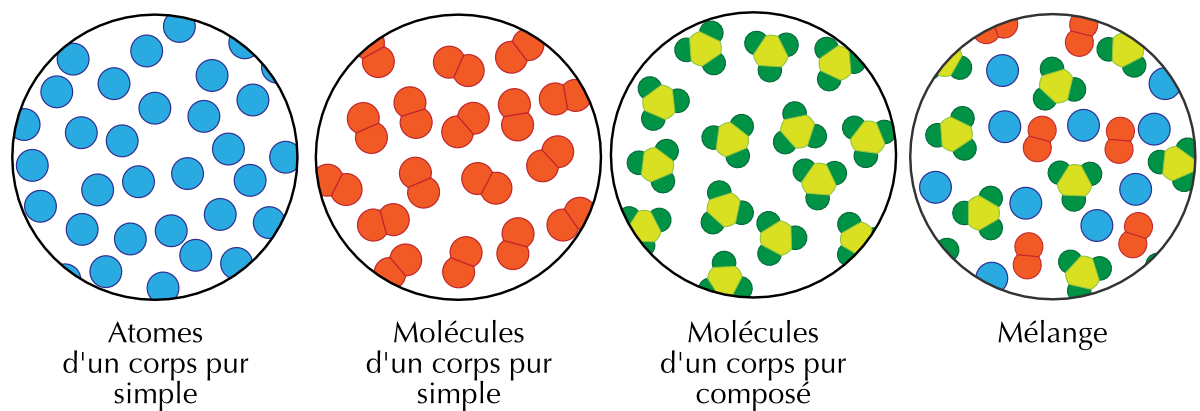
\includegraphics[width=0.67\linewidth]{images/corps-purs-corps-composes} 

}

\caption{Corps purs et corps composés}\label{fig:corps-purs-corps-composes}
\end{figure}

\hypertarget{les-muxe9langes}{%
\section{Les mélanges}\label{les-muxe9langes}}

\begin{tcolorbox}
\textbf{Mélange}\\
Ensemble résultant de l'union de substances différentes sans transformation chimique

\end{tcolorbox}

Un mélange est constitué de deux ou plusieurs substances (corps pur simples ou composés) qui sont physiquement mêlées, mais non liées chimiquement.

Les mélanges peuvent être \textbf{homogène} ou \textbf{hétérogène}. Ces deux termes sont introduits pour qualifier ce qui peut être différencié à l'oeil.

\hypertarget{les-muxe9langes-huxe9tuxe9roguxe8nes}{%
\subsection{Les mélanges hétérogènes}\label{les-muxe9langes-huxe9tuxe9roguxe8nes}}

\begin{tcolorbox}
\textbf{Mélange hétérogène}\\
Un mélange est hétérogène si on peut distinguer ses différents constituants à l'oeil nu.

\end{tcolorbox}

La composition des mélanges hétérogènes varie d'un endroit à l'autre de la matière. Par exemple, si l'on met du sucre dans un bocal, que l'on ajoute du sable et que l'on agite le bocal, le mélange n'aura pas la même composition quelque soit l'endroit du bocal.

\hypertarget{les-muxe9langes-homoguxe8nes}{%
\subsection{Les mélanges homogènes}\label{les-muxe9langes-homoguxe8nes}}

\begin{tcolorbox}
\textbf{Mélange homogène}\\
Un mélange est homogène si on ne peut pas distinguer ses différents constituants à l'oeil nu.

\end{tcolorbox}

Les mélanges homogènes ont une composition uniforme. Chaque partie d'un mélange a la même composition que n'importe quelle autre partie du même mélange. Si l'on dissout du sucre dans l'eau en mélangeant bien, le mélange sera le même, quelque soit l'endroit que l'on goûtera.

\begin{itemize}
\tightlist
\item
  L'air est un mélange homogène composé de plusieurs gaz, principalement l'azote et l'oxygène.
\item
  L'eau de mer est un mélange homogène composé principalement d'eau et de chlorure de sodium (sel).
\item
  L'essence est un mélange homogène composé d'une dizaine de substances.
\end{itemize}

\begin{figure}

{\centering 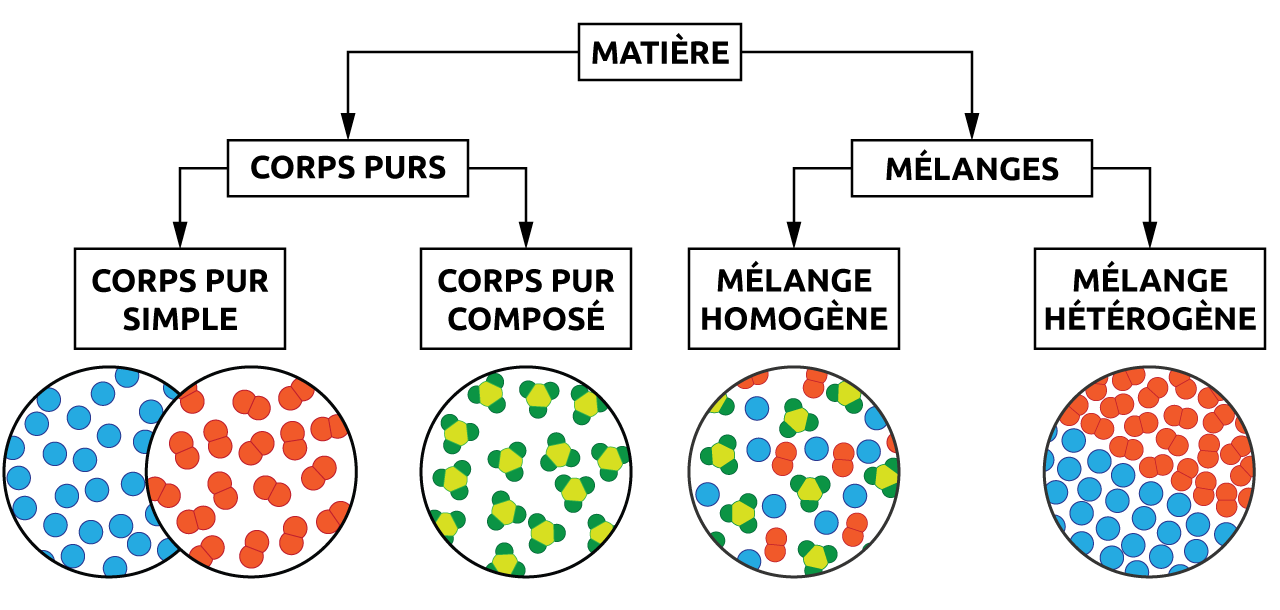
\includegraphics[width=0.67\linewidth]{images/schema-matiere} 

}

\caption{Résumé de la classification de la matière}\label{fig:schema-matiere}
\end{figure}

\begin{Exercise}

Indiquez si les échantillons suivants sont des mélanges homogènes ou hétérogènes.

\begin{enumerate}
\def\labelenumi{\arabic{enumi}.}
\tightlist
\item
  Un morceau de marbre
\item
  Un velouté de légumes
\item
  Du ciment
\item
  Un cheeseburger
\item
  Une infusion de thé
\end{enumerate}


\end{Exercise}

\begin{Answer}

\begin{enumerate}
\def\labelenumi{\arabic{enumi}.}
\tightlist
\item
  mélange hétérogène
\item
  mélange homogène
\item
  mélange homogène
\item
  mélange hétérogène
\item
  mélange homogène
\end{enumerate}


\end{Answer}

\begin{Exercise}

Indiquez si les échantillons suivants sont des corps purs, des mélanges homogènes ou des mélanges hétérogènes.

\begin{enumerate}
\def\labelenumi{\arabic{enumi}.}
\tightlist
\item
  L'eau distillée
\item
  L'essence
\item
  Le sable
\item
  Le vin
\item
  L'air
\end{enumerate}


\end{Exercise}

\begin{Answer}

\begin{enumerate}
\def\labelenumi{\arabic{enumi}.}
\tightlist
\item
  H\textsubscript{2}O - corps pur
\item
  hydrocarbures - mélange homogène
\item
  débris de roches - mélange hétérogène
\item
  eau + alcool - mélange homogène
\item
  azote + oxygène - mélange homogène
\end{enumerate}


\end{Answer}

\hypertarget{les-dispersions}{%
\subsection{Les dispersions}\label{les-dispersions}}

Les dispersions sont des mélanges homogènes dans lequel les particules en suspension sont si petites que le mélange semble parfaitement homogène à l'oeil nu. Cependant, à l'aide d'instruments d'observation, on pourra distinguer les différentes substances qui constituent les dispersions.

Les mélanges homogènes pourront à leur tour être classés en solutions, en colloïdes ou en suspensions, en fonction de la taille de leurs particules. Chaque particule peut être une macromolécule unique ou un agrégat de nombreux atomes, ions ou molécules.

\begin{itemize}
\tightlist
\item
  \textbf{Les solutions} (0.1 à 2 {[}nm{]})
  La dissolution d'une substance dans une autre forme une solution. Un mélange homogène dans lequel les particules sont individuellement réparties de manière uniforme dans la substance dispersante.
\item
  \textbf{Les colloïdes} (2 à 500 {[}nm{]})
  La substance dispersée est répartie dans la substance dispersante. Les particules sont plus grandes que des molécules simples mais trop petites pour se déposer.
\item
  \textbf{Les suspensions} (500 à 1000 {[}nm{]})
  Les particules sont d'abord en suspension mais se déposent progressivement par décantation.
\end{itemize}

Une phase représente chaque partie homogène dont est constitué une dispersion. Dans une dispersion une phase peut être dispersante et l'autre dispersée. Les dispersions sont communément classées selon l'état physique des substances dispersée et dispersante.

\begin{longtable}[]{@{}ccl@{}}
\toprule
phase dispersée & phase dispersante & suspensions et colloïdes\tabularnewline
\midrule
\endhead
gaz & gaz & mélange toujours homogène (solution)\tabularnewline
liquide & gaz & brouillard, laque pour cheveux\tabularnewline
solide & gaz & fumée, nuage, poussière\tabularnewline
gaz & liquide & crème fouettée, soda, mousse à raser\tabularnewline
liquide & liquide & lait, mayonnaise, crème solaire\tabularnewline
solide & liquide & peinture, sang, boue\tabularnewline
gaz & solide & polystyrène, pierre ponce\tabularnewline
liquide & solide & agar-agar, gelatine\tabularnewline
solide & solide & roches naturelles, plâtre, ciment, béton\tabularnewline
\bottomrule
\end{longtable}

\newpage

\hypertarget{muxe9thodes-de-suxe9paration}{%
\section{Méthodes de séparation}\label{muxe9thodes-de-suxe9paration}}

Les constituants d'un mélange ont des \textbf{propriétés physiques} différentes. On peut exploiter ces différences pour séparer les différents constituants.

Les techniques décrites ne dépendent que des propriétés physiques des constituants. Il n'y a pas de transformation chimiques qui se produit.

\hypertarget{lattraction-magnuxe9tique}{%
\subsection{L'attraction magnétique}\label{lattraction-magnuxe9tique}}

\begin{figure}

{\centering 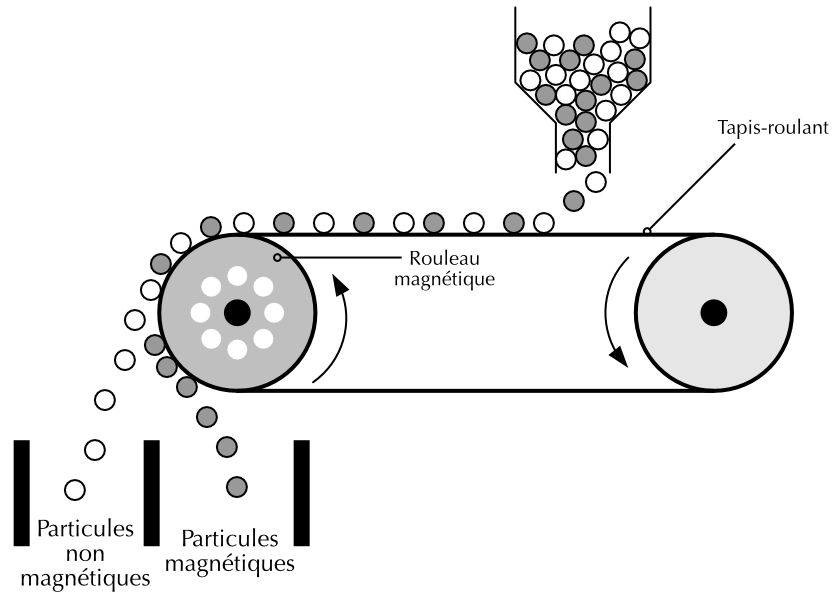
\includegraphics[width=0.38\linewidth]{images/attraction-magnetique} 

}

\caption{Séparation par attraction magnétique}\label{fig:attraction-magnetique}
\end{figure}

L'\textbf{attraction magnétique}, ou \textbf{aimantation}, utilise les différences de \textbf{propriétés magnétiques}. Elle permet de séparer un mélange de substances magnétiques et non-magnétiques.

Un mélange de limaille de fer et de poudre de soufre peut être séparé en utilisant un aimant. Cette technique est utilisée dans les déchetteries pour séparer les matériaux magnétiques des matériaux non-magnétiques.

\hypertarget{la-filtration}{%
\subsection{La filtration}\label{la-filtration}}

\begin{figure}

{\centering 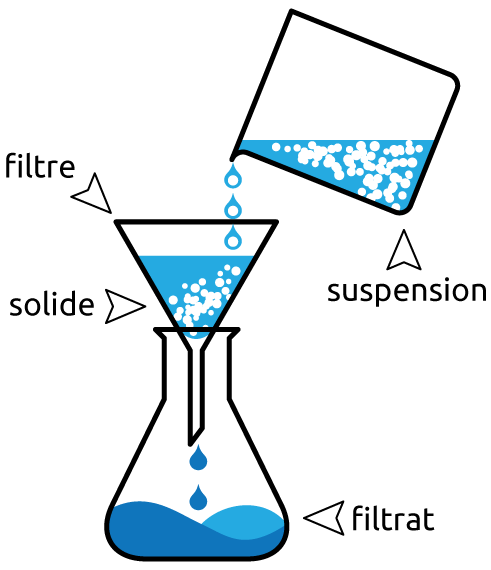
\includegraphics[width=0.28\linewidth]{images/filtration} 

}

\caption{Filtration par gravité}\label{fig:filtration}
\end{figure}

La filtration est basée sur la \textbf{différence de taille des particules}. Elle est souvent utilisée pour séparer un solide d'un liquide. Le liquide s'écoule à travers les petits trous dans le filtre alors que le solide est retenu.

Dans la filtration sous vide, on diminue la pression au-dessous du filtre ce qui accélère l'écoulement du liquide.

\newpage

\hypertarget{la-vaporisation}{%
\subsection{La vaporisation}\label{la-vaporisation}}

\begin{figure}

{\centering 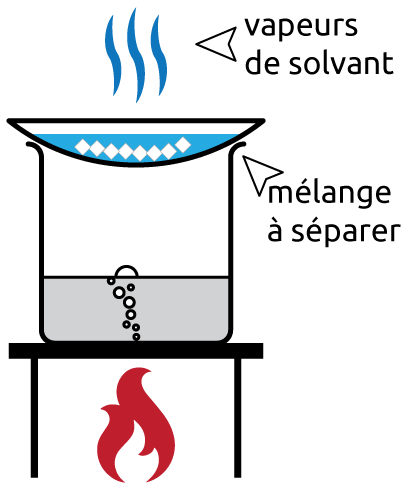
\includegraphics[width=0.25\linewidth]{images/evaporation} 

}

\caption{Vaporisation}\label{fig:evaporation}
\end{figure}

La vaporisation est basée sur les \textbf{différences de points d'ébullition}. Cette technique est utilisée pour séparer des solides dissous dans un solvant.

Lorsque le mélange contenant les matières solides dissoutes est chauffé, le solvant (liquide) vaporise progressivement et le soluté (solide) solidifie dans le récipient.

Le terme \textbf{évaporation} est utilisé lorsque l'eau est le liquide qui vaporise.

\hypertarget{la-dissolution-suxe9lective}{%
\subsection{La dissolution sélective}\label{la-dissolution-suxe9lective}}

\vspace{\stretch{1}}

\begin{figure}

{\centering 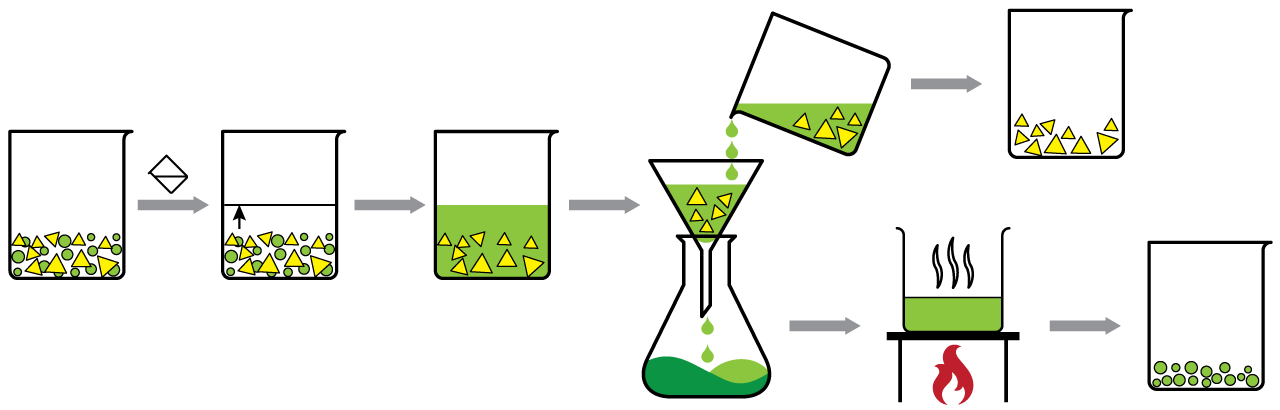
\includegraphics[width=0.85\linewidth]{images/dissolution-selective} 

}

\caption{Dissolution sélective}\label{fig:dissolution-selective}
\end{figure}

\vspace{\stretch{1}}

La dissolution sélective est basée sur les \textbf{différences de solubilité}.

Cette technique permet de séparer deux solides en ajoutant un solvant dans lequel un seul solide se dissout. Ensuite, il faut filtrer le mélange et vaporiser le solvant afin de récupérer les deux solides.

\newpage

\hypertarget{la-sublimation}{%
\subsection{La sublimation}\label{la-sublimation}}

\begin{figure}

{\centering 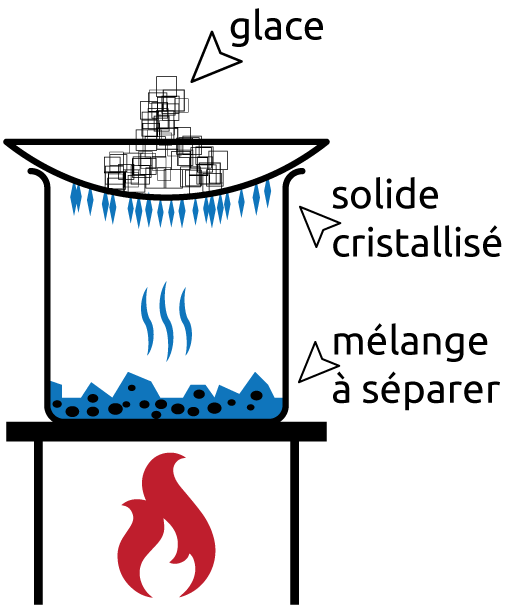
\includegraphics[width=0.28\linewidth]{images/sublimation} 

}

\caption{Sublimation}\label{fig:sublimation}
\end{figure}

La sublimation est une technique de séparation dans laquelle une substance dans un mélange est directement transformée à l'état gazeux sans passer par l'état liquide. Par chauffage, la matière solide sublime et se solidifie à nouveau lorsque les vapeurs entrent en contact avec une surface froide.

Certains composés solides, tels que l'iode, le camphre, le naphtalène, l'acétanilide, l'acide benzoïque, peuvent être purifiés par sublimation à pression normale. D'autres composés, comme par exemple la caféine, devront être sublimés par chauffage sous pression réduite.

\hypertarget{la-distillation}{%
\subsection{La distillation}\label{la-distillation}}

\begin{figure}

{\centering 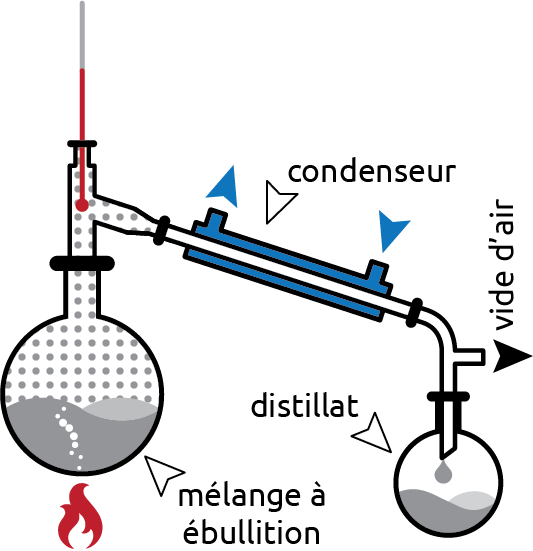
\includegraphics[width=0.4\linewidth]{images/distillation} 

}

\caption{Distillation simple}\label{fig:distillation}
\end{figure}

La distillation est la principale méthode de séparation des mélanges constitués de liquides. Elle est basée sur la \textbf{différence des températures d'ébullition} des constituants du mélange.

La solution est chauffée de sorte que le liquide ayant le point d'ébullition le plus bas se transforme en vapeur. La vapeur s'élève alors, et se dirige vers le condenseur, où elle est refroidie. La vapeur condense alors en un liquide appelé distillat.

\hypertarget{la-chromatographie}{%
\subsection{La chromatographie}\label{la-chromatographie}}

\begin{figure}

{\centering 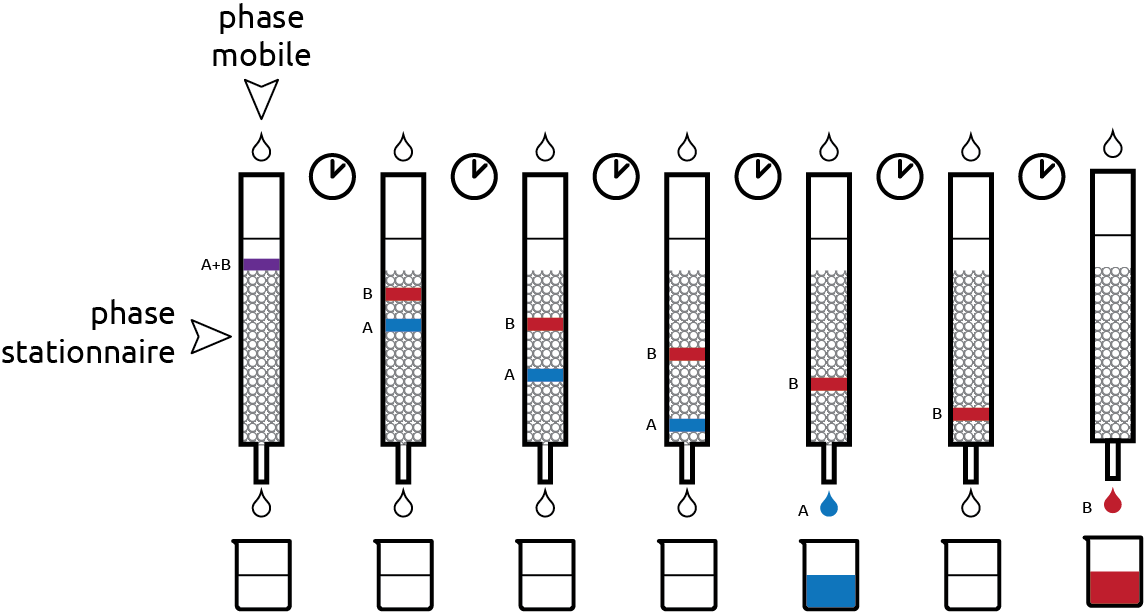
\includegraphics[width=0.67\linewidth]{images/chromatographie} 

}

\caption{Chromatographie sur colonne}\label{fig:chromatographie}
\end{figure}

La chromatographie est basée sur le fait que les composants d'un mélange ont plus ou moins tendance à être retenus sur une surface solide.

Cette méthode se compose d'une partie statique (phase stationnaire) et d'une partie mobile (phase mobile). La phase mobile se déplace à travers la phase stationnaire. On injecte le mélange à séparer dans la phase mobile afin qu'il se déplace avec cette dernière dans la phase stationnaire. Les constituants du mélange ayant des affinités différentes avec les deux phases vont se déplacer plus ou moins vite et ainsi être séparés.

\hypertarget{lextraction}{%
\subsection{L'extraction}\label{lextraction}}

\begin{figure}

{\centering 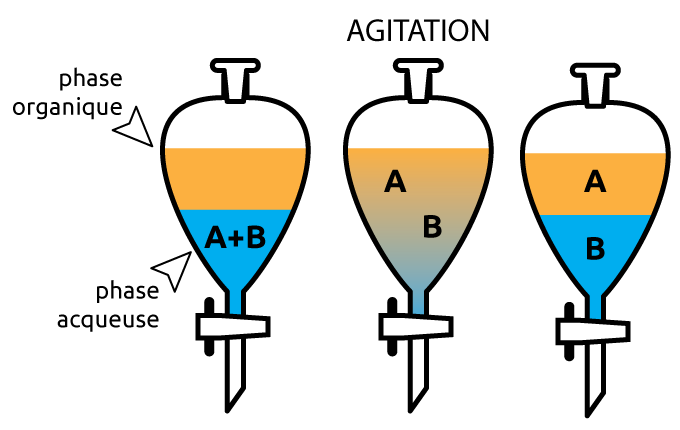
\includegraphics[width=0.45\linewidth]{images/extraction} 

}

\caption{Extraction}\label{fig:extraction}
\end{figure}

L'extraction est basée sur les \textbf{différences de solubilités}.

On utilise généralement deux solvants ayant une polarité différente, comme l'eau et un solvant organique. Les différentes substances vont migrer dans le solvant dans lequel elles ont la plus grande solubilité.

\newpage

\hypertarget{la-suxe9dimentation-et-la-duxe9cantation}{%
\subsection{La sédimentation et la décantation}\label{la-suxe9dimentation-et-la-duxe9cantation}}

\begin{figure}

{\centering 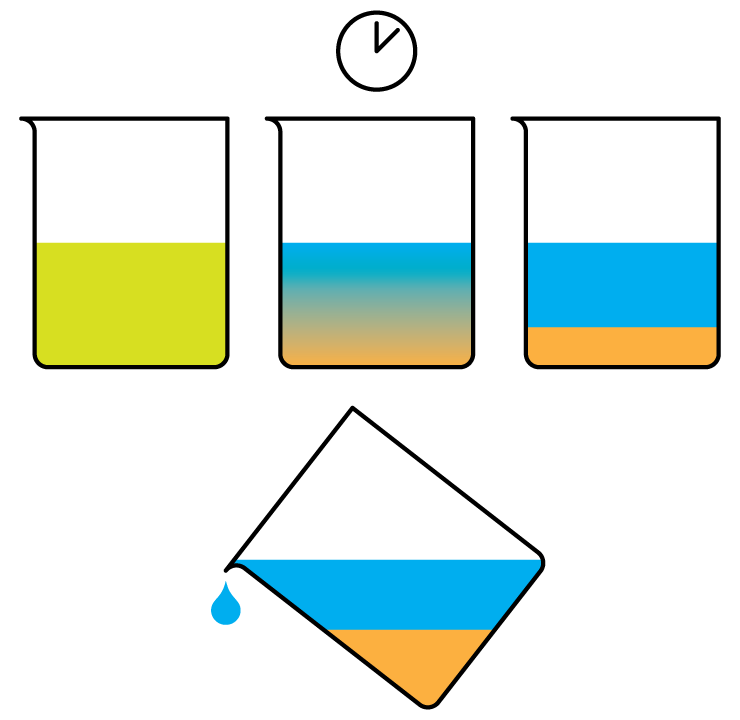
\includegraphics[width=0.33\linewidth]{images/sedimentation} 

}

\caption{Sédimentation}\label{fig:sedimentation}
\end{figure}

La \textbf{sédimentation} est un processus dans lequel on laisse couler des particules lourdes insolubles dans un liquide par gravitation. Le liquide clair obtenu est ensuite transféré dans un autre récipient, sans déranger les particules sédimentées. Ce transfert s'appelle la \textbf{décantation}.

La sédimentation et la décantation peuvent également être utilisées pour séparer un mélange de liquides lorsqu'ils ne sont pas miscibles.

La \textbf{centrifugation} utilise la force centrifuge pour accélérer la sédimentation. Les composants plus denses migrent loin de l'axe de la centrifugeuse, tandis que les composants moins denses du mélange migrent vers l'axe.

\newpage

\begin{Exercise}

Quelle méthode de séparation est employée dans chacune des procédures suivantes ?

\begin{enumerate}
\def\labelenumi{\arabic{enumi}.}
\tightlist
\item
  Verser un mélange de pâtes cuites et d'eau bouillante dans une passoire.
  \vspace{\stretch{1}}
\item
  L'élimination des impuretés colorées dans le sucre brun pour en faire du sucre raffiné.
  \vspace{\stretch{1}}
\item
  La récupération du sel de table dans des bassins de faible profondeur après évaporation de l'eau de mer, sous l'action combinée du soleil et du vent.
  \vspace{\stretch{1}}
\end{enumerate}


\end{Exercise}

\begin{Answer}

\begin{enumerate}
\def\labelenumi{\arabic{enumi}.}
\tightlist
\item
  Filtration
\item
  Cristallisation
\item
  Vaporisation / Évaporation
\end{enumerate}


\end{Answer}

\hypertarget{ruxe9sumuxe9-des-muxe9thodes-de-suxe9paration}{%
\subsection{Résumé des méthodes de séparation}\label{ruxe9sumuxe9-des-muxe9thodes-de-suxe9paration}}

\begin{longtable}[]{@{}ccl@{}}
\toprule
\begin{minipage}[b]{0.19\columnwidth}\centering
mélange à séparer\strut
\end{minipage} & \begin{minipage}[b]{0.28\columnwidth}\centering
méthode de séparation\strut
\end{minipage} & \begin{minipage}[b]{0.44\columnwidth}\raggedright
Propriété utilisée\strut
\end{minipage}\tabularnewline
\midrule
\endhead
\begin{minipage}[t]{0.19\columnwidth}\centering
solide/solide\strut
\end{minipage} & \begin{minipage}[t]{0.28\columnwidth}\centering
attraction magnétique\strut
\end{minipage} & \begin{minipage}[t]{0.44\columnwidth}\raggedright
un composant est magnétique\strut
\end{minipage}\tabularnewline
\begin{minipage}[t]{0.19\columnwidth}\centering
solide/solide\strut
\end{minipage} & \begin{minipage}[t]{0.28\columnwidth}\centering
dissolution sélective\strut
\end{minipage} & \begin{minipage}[t]{0.44\columnwidth}\raggedright
un composant est soluble\strut
\end{minipage}\tabularnewline
\begin{minipage}[t]{0.19\columnwidth}\centering
solide/solide\strut
\end{minipage} & \begin{minipage}[t]{0.28\columnwidth}\centering
sublimation\strut
\end{minipage} & \begin{minipage}[t]{0.44\columnwidth}\raggedright
un composant sublime\strut
\end{minipage}\tabularnewline
\begin{minipage}[t]{0.19\columnwidth}\centering
solide/solide\strut
\end{minipage} & \begin{minipage}[t]{0.28\columnwidth}\centering
chromatographie\strut
\end{minipage} & \begin{minipage}[t]{0.44\columnwidth}\raggedright
affinité avec la phase stationnaire\strut
\end{minipage}\tabularnewline
\begin{minipage}[t]{0.19\columnwidth}\centering
solide/solide\strut
\end{minipage} & \begin{minipage}[t]{0.28\columnwidth}\centering
extraction\strut
\end{minipage} & \begin{minipage}[t]{0.44\columnwidth}\raggedright
solubilité dans un des solvants\strut
\end{minipage}\tabularnewline
\begin{minipage}[t]{0.19\columnwidth}\centering
\strut
\end{minipage} & \begin{minipage}[t]{0.28\columnwidth}\centering
\strut
\end{minipage} & \begin{minipage}[t]{0.44\columnwidth}\raggedright
\strut
\end{minipage}\tabularnewline
\begin{minipage}[t]{0.19\columnwidth}\centering
solide/liquide\strut
\end{minipage} & \begin{minipage}[t]{0.28\columnwidth}\centering
filtration\strut
\end{minipage} & \begin{minipage}[t]{0.44\columnwidth}\raggedright
taille des particules\strut
\end{minipage}\tabularnewline
\begin{minipage}[t]{0.19\columnwidth}\centering
solide/liquide\strut
\end{minipage} & \begin{minipage}[t]{0.28\columnwidth}\centering
vaporisation\strut
\end{minipage} & \begin{minipage}[t]{0.44\columnwidth}\raggedright
température d'ébullition / volatilité\strut
\end{minipage}\tabularnewline
\begin{minipage}[t]{0.19\columnwidth}\centering
solide/liquide\strut
\end{minipage} & \begin{minipage}[t]{0.28\columnwidth}\centering
sédimentation/décantation\strut
\end{minipage} & \begin{minipage}[t]{0.44\columnwidth}\raggedright
masse volumique / taille des particules\strut
\end{minipage}\tabularnewline
\begin{minipage}[t]{0.19\columnwidth}\centering
\strut
\end{minipage} & \begin{minipage}[t]{0.28\columnwidth}\centering
\strut
\end{minipage} & \begin{minipage}[t]{0.44\columnwidth}\raggedright
\strut
\end{minipage}\tabularnewline
\begin{minipage}[t]{0.19\columnwidth}\centering
liquide/liquide\strut
\end{minipage} & \begin{minipage}[t]{0.28\columnwidth}\centering
distillation\strut
\end{minipage} & \begin{minipage}[t]{0.44\columnwidth}\raggedright
température d'ébullition\strut
\end{minipage}\tabularnewline
\begin{minipage}[t]{0.19\columnwidth}\centering
liquide/liquide\strut
\end{minipage} & \begin{minipage}[t]{0.28\columnwidth}\centering
chromatographie\strut
\end{minipage} & \begin{minipage}[t]{0.44\columnwidth}\raggedright
affinité avec la phase stationnaire\strut
\end{minipage}\tabularnewline
\begin{minipage}[t]{0.19\columnwidth}\centering
liquide/liquide\strut
\end{minipage} & \begin{minipage}[t]{0.28\columnwidth}\centering
extraction\strut
\end{minipage} & \begin{minipage}[t]{0.44\columnwidth}\raggedright
solubilité dans un des solvants\strut
\end{minipage}\tabularnewline
\bottomrule
\end{longtable}

\newpage

\hypertarget{exercices-suppluxe9mentaires-2}{%
\section{Exercices supplémentaires}\label{exercices-suppluxe9mentaires-2}}

\begin{Exercise}

Indiquez si chaque échantillon de matière indiqué est un corps pur, un corps composé, un mélange homogène ou un mélange hétérogène.

\begin{enumerate}
\def\labelenumi{\arabic{enumi}.}
\tightlist
\item
  une cuillère en argent
  \vspace{\stretch{1}}
\item
  un pain au chocolat
  \vspace{\stretch{1}}
\item
  un glaçon
  \vspace{\stretch{1}}
\item
  une poutre en bois
  \vspace{\stretch{1}}
\item
  de l'encre rouge
  \vspace{\stretch{1}}
\item
  du jus d'orange pressé
  \vspace{\stretch{1}}
\end{enumerate}


\end{Exercise}

\begin{Answer}

\begin{enumerate}
\def\labelenumi{\arabic{enumi}.}
\tightlist
\item
  corps pur simple
\item
  mélange hétérogène
\item
  corps purs composé
\item
  mélange hétérogène
\item
  mélange homogène
\item
  mélange hétérogène
\end{enumerate}


\end{Answer}

\begin{Exercise}

Proposer une méthode de séparation par laquelle les mélanges suivants peuvent être séparés.

\begin{enumerate}
\def\labelenumi{\arabic{enumi}.}
\tightlist
\item
  de la limaille de fer et des copeaux de bois
  \vspace{\stretch{1}}
\item
  des éclats de verre et du saccharose (sucre de canne)
  \vspace{\stretch{1}}
\item
  de l'eau et de l'huile d'olive
  \vspace{\stretch{1}}
\item
  des paillettes d'or et de l'eau
  \vspace{\stretch{1}}
\end{enumerate}


\end{Exercise}

\begin{Answer}

\begin{enumerate}
\def\labelenumi{\arabic{enumi}.}
\tightlist
\item
  attraction magnétique
\item
  dissolution sélective ou recristallisation
\item
  sédimentation - décantation
\item
  filtration
\end{enumerate}


\end{Answer}

\newpage

\section{Solutions des exercices} \shipoutAnswer

\hypertarget{historique}{%
\chapter{Historique}\label{historique}}

\begin{objectives}

\begin{itemize}
\tightlist
\item
  Décrire le processus par lequel les éléments chimiques ont été créés.
\item
  Décrire les expériences clés et les principales hypothèses qui ont conduit à la découverte du modèle atomique.
\end{itemize}


\end{objectives}

Selon le modèle du \textbf{Big Bang}, l'Univers est né il y a environ 14 milliards d'années lors d'une explosion cataclysmique. Cette explosion marque le début de l'espace, du temps, de la matière et de l'expansion de l'Univers. Quelques milliardièmes de seconde après le Big Bang, l'univers était constitué d'une sorte de soupe primordiale extrêmement chaude et dense des particules les plus fondamentales. L'univers se refroidit sous la barre des 1013 degrés et ces particules fondamentales commencent à s'assembler pour former protons et neutrons. Entre une et trois secondes après le Big Bang apparaît l'époque de la nucléosynthèse primordiale qui va durer environ 3 minutes. C'est à ce moment que se produit la formation de noyaux atomiques à partir des protons et neutrons qui étaient jusque-là libres.

\hypertarget{les-origines-de-la-matiuxe8re}{%
\section{Les origines de la matière}\label{les-origines-de-la-matiuxe8re}}

Le processus par lequel des éléments chimiques sont créés est appelé \textbf{nucléosynthèse}. On distingue plusieurs types de nucléosynthèses:

\begin{itemize}
\item
  \textbf{la nucléosynthèse primordiale}\\
  Le Big Bang a créé toute la matière et l'énergie de l'Univers. L'hydrogène et l'hélium sont créés dans les instants qui suivent le Big Bang.
\item
  \textbf{la nucléosynthèse stellaire}\\
  De petites étoiles fusionnent l'hydrogène en hélium, puis fusionnent l'hélium en carbone et en azote. Dans le coeur de plus grandes étoiles les éléments plus lourds sont formés comme le calcium, l'oxygène, le silicium, le soufre ou le fer.
\item
  \textbf{la nucléosynthèse explosive}\\
  L'explosion de supernovas crée et disperse un grand nombre d'éléments plus lourds que le fer. Lors de ces explosions la matière est dispersée dans l'univers.
\item
  \textbf{la nucléosynthèse interstellaire}\\
  La matière créée lors du Big Bang ou dans les étoiles est bombardée en permanence par les rayons cosmiques. Ce bombardement mène à des réactions de fission nucléaire qui créent à nouveau des éléments plus légers comme le lithium, le bore et ou béryllium.
\end{itemize}

\newpage

\begin{figure}

{\centering 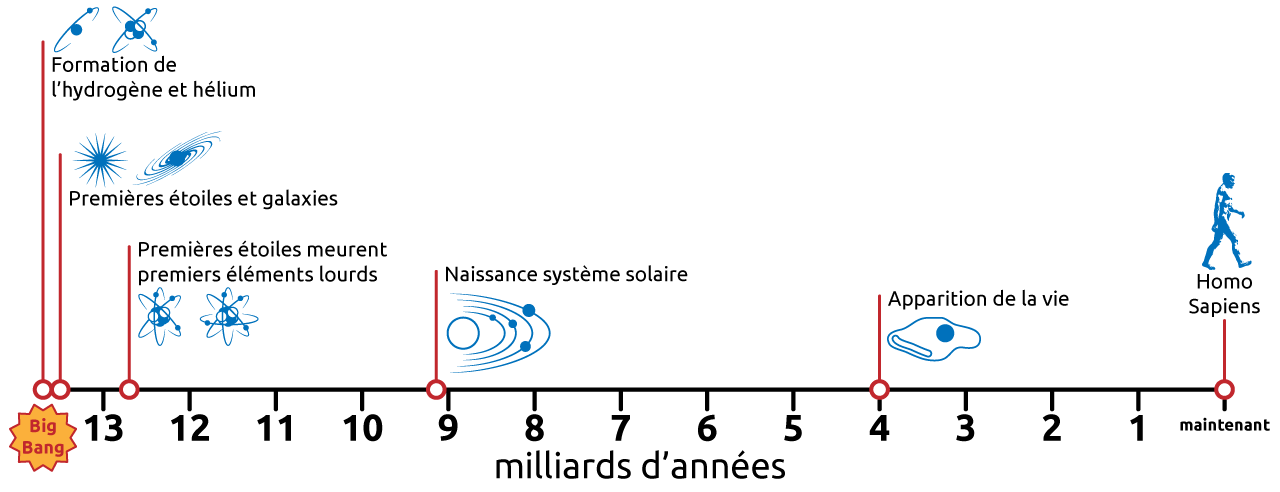
\includegraphics[width=0.8\linewidth]{images/timeline-cosmos} 

}

\caption{Chronologie du cosmos}\label{fig:timeline-cosmos}
\end{figure}

\hypertarget{le-moduxe8le-atomique}{%
\section{Le modèle atomique}\label{le-moduxe8le-atomique}}

Autour du 5 siècle avant JC, le philosophe grec \textbf{Démocrite} est le premier à décrire le concept d'\textbf{atome} (atomos signifie indivisible en grec). Pour Démocrite, l'atome est éternel, constant, invisible et indivisible. Il est la plus petite unité et le bloc de construction de toute matière.

Les philosophes \textbf{Platon} et \textbf{Aristote} s'opposèrent fortement à l'idée de Démocrite, affirmant que la matière avait une structure continue que l'on pouvait diviser à l'infini. Il faudra attendre près de 2000 ans pour que la science puisse prouver que Démocrite avait raison!

Au début du 19e siècle, \textbf{John Dalton} (1766-1844) développe ce qui est maintenant considéré comme le fondement de la théorie atomique moderne. Dalton base sa théorie sur 5 hypothèses:

\begin{itemize}
\tightlist
\item
  La matière est faite de très petites particules appelées \textbf{atomes} qui ne peuvent pas être subdivisés ou détruits.
\item
  Tous les atomes d'un même élément sont identiques.
\item
  Les atomes d'éléments différents ont des masses différentes.
\item
  Les atomes peuvent se combiner entre eux pour former des composés.
\item
  Une réaction chimique est une modification de l'arrangement d'un groupe d'atomes.
\end{itemize}

En 1897, le physicien britannique \textbf{Joseph John Thomson} (1856-1940) découvre l'\textbf{électron}, une très petite particule chargée négativement. L'expérience menée par Thomson l'a conduit à la conclusion que l'électron est une particule constituante de l'atome. Comme les atomes sont électriquement neutres, de la matière chargée positivement doit exister. Thomson propose un nouveau modèle de l'atome. Il est constitué d'une masse de matière de charge positive avec des électrons de charge négative coincés dedans. Ce modèle est appelé le modèle pain de raisin (plum pudding).

\begin{figure}

{\centering 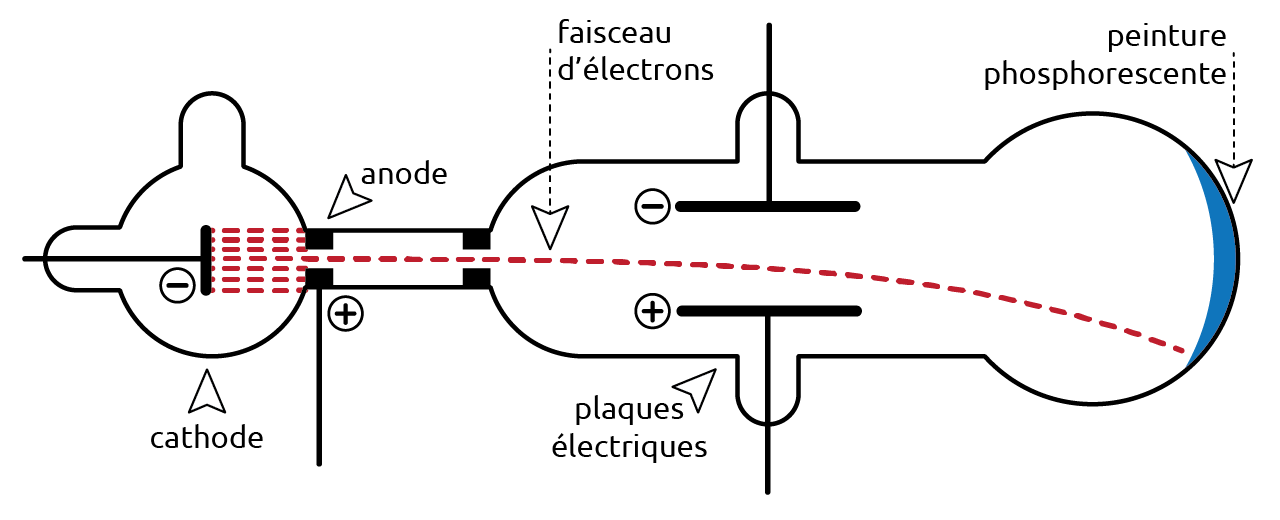
\includegraphics[width=0.4\linewidth]{images/exp-thomson} 

}

\caption{Schéma du tube cathodique de Thomson}\label{fig:exp-thomson}
\end{figure}

En 1911, le physicien britannique \textbf{Ernest Rutherford} (1871-1937) fait une découverte importante. Il bombarde une feuille d'or extrêmement fine avec des particules alpha. Les particules alpha sont des particules radioactives chargées positivement.

\begin{figure}

{\centering 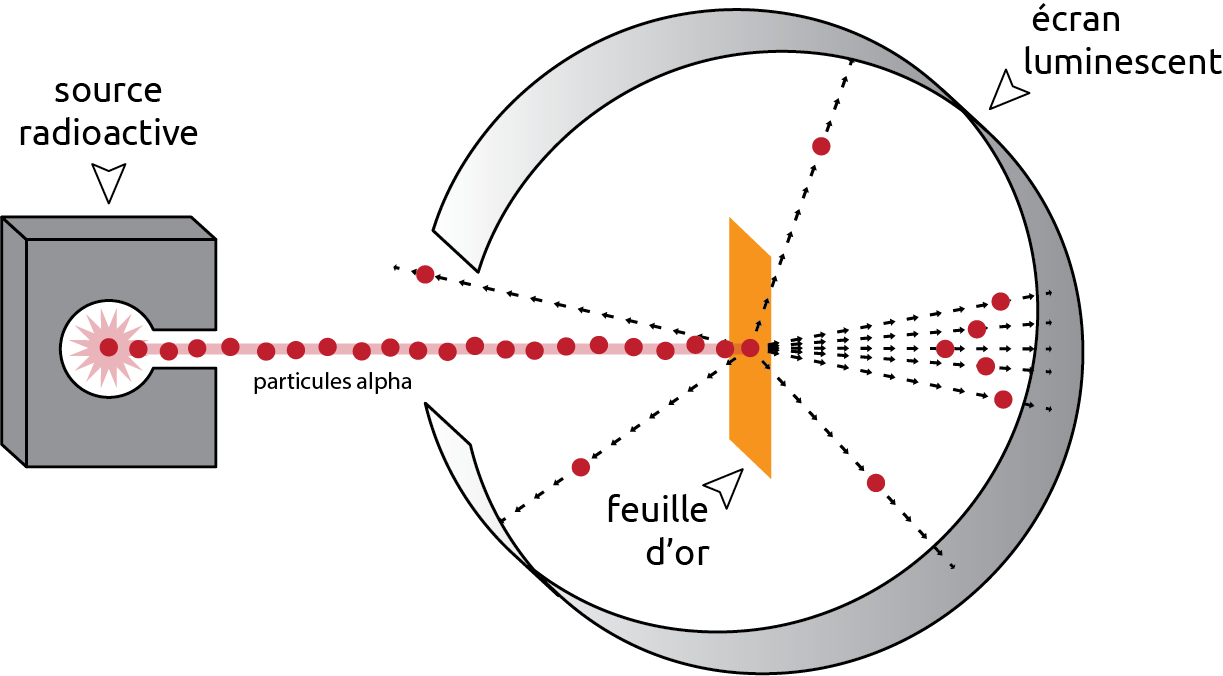
\includegraphics[width=0.4\linewidth]{images/exp-rutherford} 

}

\caption{Bombardement de la feuille d'or}\label{fig:exp-rutherford}
\end{figure}

Selon le modèle de Thomson, toutes les particules alpha devaient passer à travers la feuille d'or sans entrave. La plupart des particules ont effectivement passé à travers la feuille, mais certaines rebondissaient comme si elles avaient frappé un objet massif positif. Rutherford conclu que la charge positive et la plupart de la masse de l'atome sont concentrées dans un très petit volume: le \textbf{noyau}. Rutherford a proposé un nouveau modèle de l'atome appelé modèle planétaire, avec un noyau au centre et des électrons gravitant autour du noyau comme les planètes autour du soleil.

\begin{figure}

{\centering 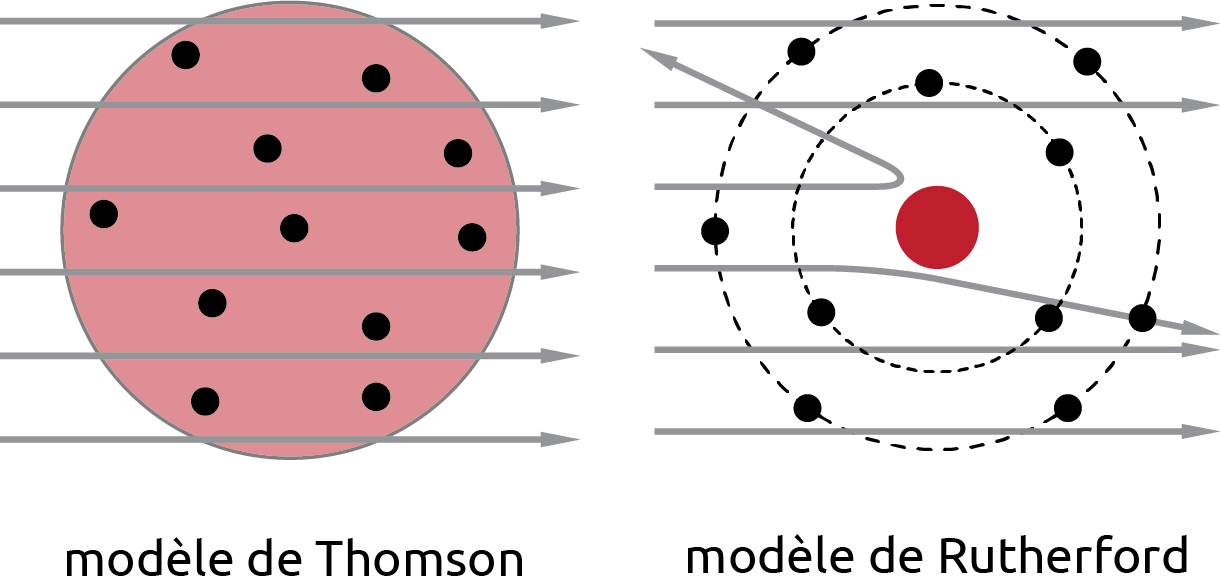
\includegraphics[width=0.4\linewidth]{images/exp-thomson-rutherford} 

}

\caption{Comparaison des modèles de Thomson et de Rutherford}\label{fig:exp-thomson-rutherford}
\end{figure}

En 1913, le physicien danois \textbf{Niels Henrik David Bohr} (1885-1962), propose un nouveau modèle de l'atome. Selon ce modèle, les électrons peuvent se déplacer sur des orbites à une distance spécifique du noyau, car l'énergie qu'ils possèdent n'est pas continue mais quantifiée.

En 1932, le physicien \textbf{James Chadwick} (1891-1974) découvre la troisième particule subatomique, le \textbf{neutron}. Un neutron a une masse très proche de celle du proton mais il n'a pas de charge électrique.

Deux même charges se repoussent mutuellement. Donc, si tous les protons dans le noyau se repoussent, pourquoi le noyau n'éclate-t-il pas tout simplement? \textbf{C'est la force nucléaire}. La force nucléaire est une force qui s'exerce entre protons et neutrons. Les neutrons stabilisent le noyau car ils ajoutent de l'attraction nucléaire sans provoquer de répulsion électrique.

\begin{figure}

{\centering 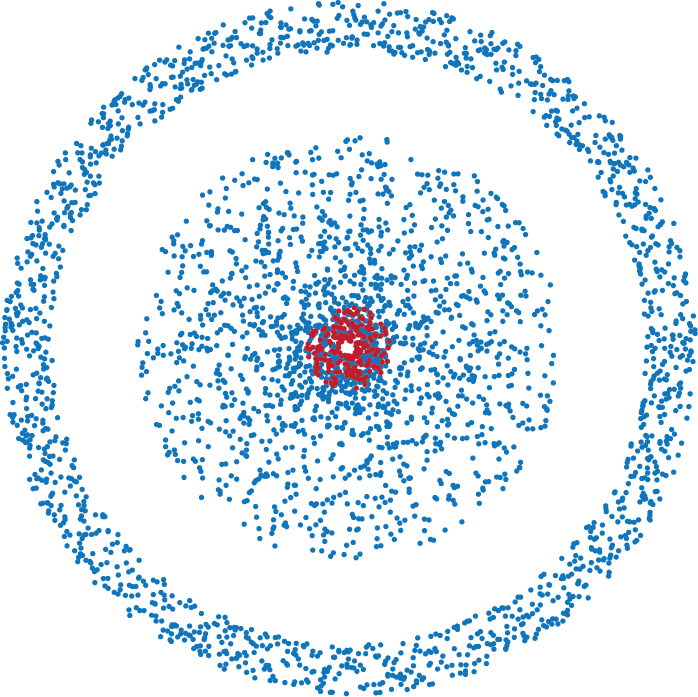
\includegraphics[width=0.25\linewidth]{images/modeles-atomiques-cloud} 

}

\caption{Le modèle standard}\label{fig:modeles-atomiques-cloud}
\end{figure}

Le modèle du nuage électronique a été développé en 1925 par \textbf{Erwin Schrödinger} (1887-1961) et \textbf{Werner Heisenberg} (1901-1976). Le \textbf{nuage électronique} représente la probabilité de trouver un électron dans une région de l'espace autour du noyau. Le nuage est plus dense aux endroits où la probabilité de trouver un électron est plus élevée.

La notion de probabilité a été introduite car on ne peut pas connaître simultanément la position et la vitesse d'un électron.

On peut faire une analogie entre le nuage électronique et l'hélice d'un avion. Quand le moteur de l'avion est arrêté, on peut voir les pales de l'hélice. Quand le moteur est allumé, les pales de l'hélices se déplacent si rapidement qu'on ne voit qu'une trace circulaire. Vous savez que les pales se trouvent quelque part dans la trace, mais à un instant donné, vous ne pouvez pas connaître précisément la position d'une pale.

Développé au début des années 1970, le \textbf{modèle standard} est le modèle actuellement accepté. Il a permis d'expliquer avec succès presque tous les résultats expérimentaux et de prédire avec précision une grande variété de phénomènes.

\begin{figure}

{\centering 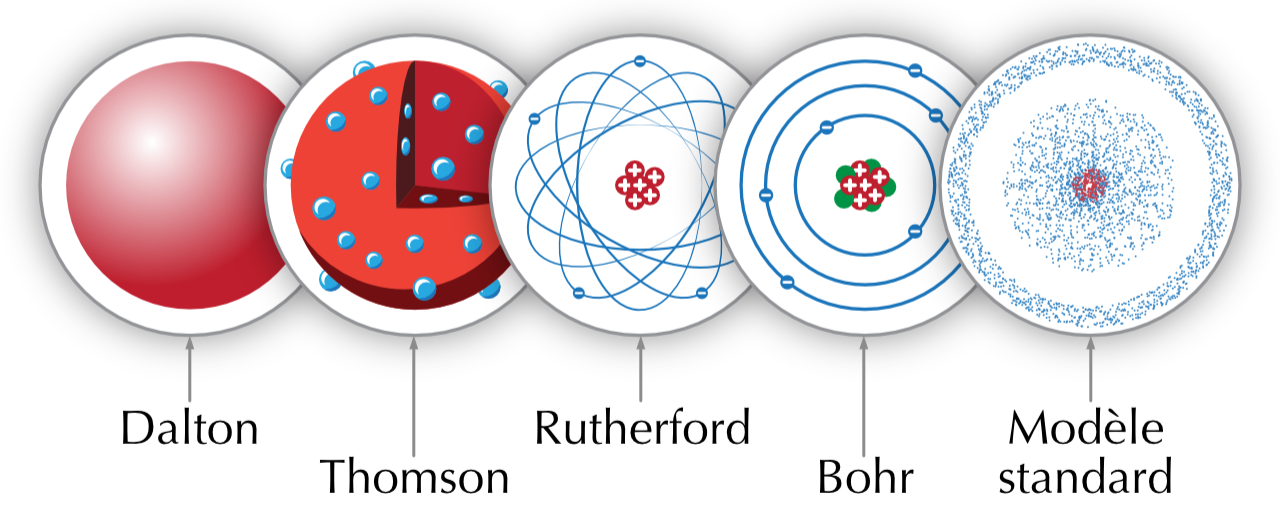
\includegraphics[width=0.85\linewidth]{images/modeles-atomiques-evol-3} 

}

\caption{Évolution du modèle atomique}\label{fig:modeles-atomiques-evol-3}
\end{figure}

Chaque modèle a ses mérites mais un modèle est, au mieux, une solution temporaire. Les modèles sont des sujets de recherche et changent avec le temps. Parfois, les anciens modèles sont mis de côté, mais ils conservent leur pouvoir explicatif et restent utiles.

Dans le cadre de ce cours, nous utiliseront le modèle de Bohr. Ce modèle nous permettra de décrire les différents sujets et phénomènes auxquels nous seront confrontés.

\newpage

\hypertarget{uxe9chelle-des-tailles}{%
\section{Échelle des tailles}\label{uxe9chelle-des-tailles}}

La taille d'un atome est difficile à mesurer car les atomes n'ont pas une limite extérieure bien définie. Cependant, on sait que leur taille est d'environ 0.1 {[}nm{]} jusqu'à 0.215 {[}nm{]} pour les plus gros. Les longueurs d'onde de la lumière visible à l'oeil humain se situent entre 400 {[}nm{]} à 700 {[}nm{]}, ce qui est trop grand pour pouvoir voir les atomes avec un procédé utilisant la lumière visible.

\begin{figure}

{\centering 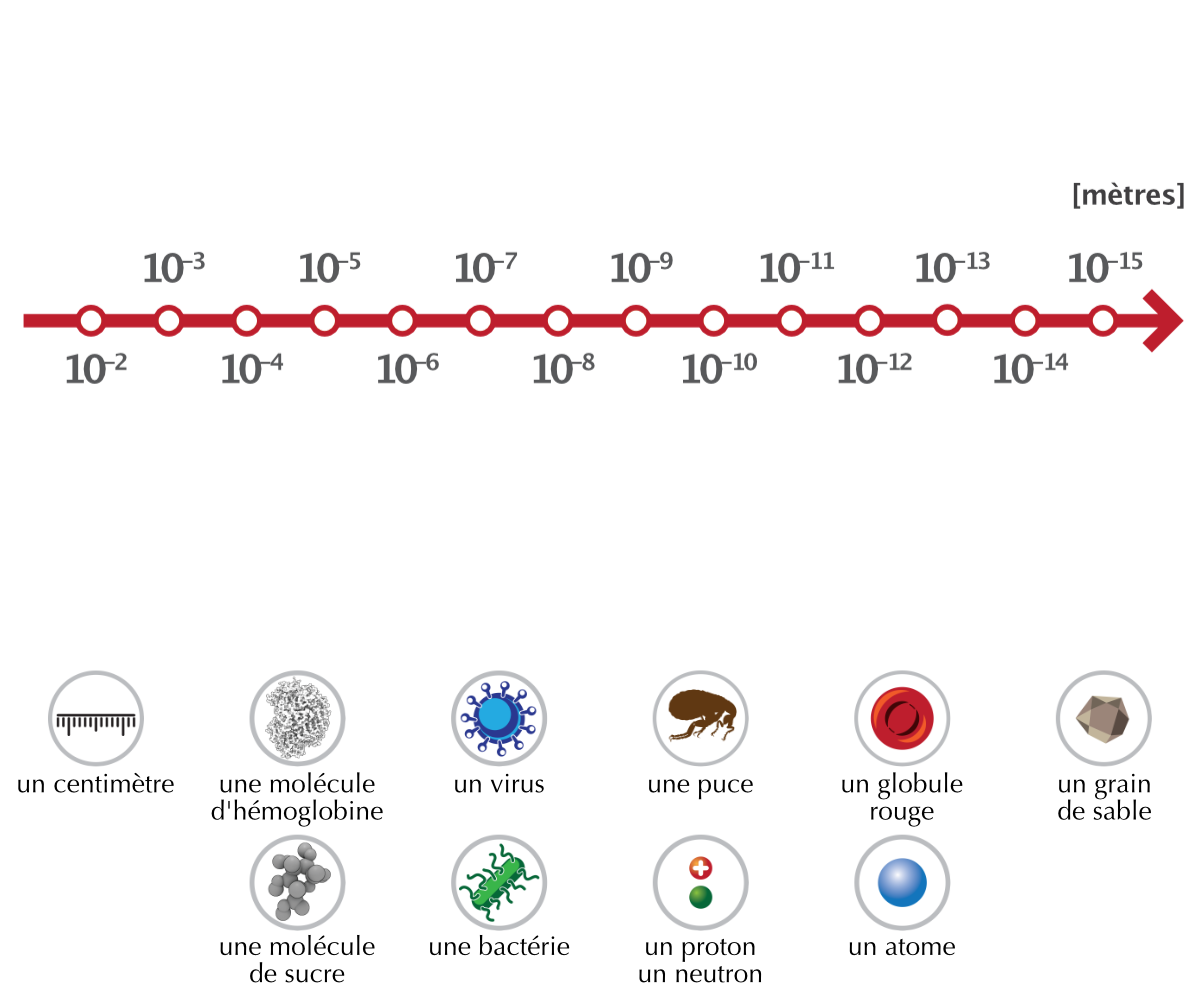
\includegraphics[width=1\linewidth]{images/ordre-grandeur-ex} 

}

\caption{Tailles relatives approximatives en mètres}\label{fig:ordre-grandeur-ex}
\end{figure}

Voir les atomes nécessite une variété d'instruments de pointe qui utilisent différents types de particules ou de rayonnements. Les rayons X, les neutrons et les électrons fournissent des informations complémentaires. Ces techniques permettent de se représenter de manière indirecte ce à quoi peut ressembler un atome.

\hypertarget{latome}{%
\chapter{L'atome}\label{latome}}

\begin{objectives}

\begin{itemize}
\tightlist
\item
  Décrire la structure de l'atome en termes de protons, de neutrons et d'électrons.
\item
  Décrire les charges électriques et les masses relatives des protons, des neutrons et des électrons.
\item
  Utiliser les symboles chimiques ainsi que le numéro atomique et le nombre de masse pour exprimer la composition subatomique des isotopes.
\item
  Définir l'unité de masse atomique. Décrire et calculer le défaut de masse.
\item
  Convertir un nombre en moles et vice versa en utilisant le nombre d'Avogadro.
\item
  Calculer la masse atomique d'un élément, en uma ou en g/mol, à partir des masses de ses isotopes et de leurs abondances naturelles.
\end{itemize}


\end{objectives}

\begin{tcolorbox}
\textbf{Atome}\\
Un atome est la plus petite particule d'un élément qui conserve encore les propriétés de cet élément.

\end{tcolorbox}

L'atome est formé d'un nuage d'électrons gravitant autour d'un petit noyau extrêmement dense. Le noyau atomique contient les protons qui sont chargés positivement et les neutrons qui ne sont pas chargés. Les électrons, qui sont chargés négativement, se déplacent autour du noyau sur des trajectoires complexes, qui forment le nuage électronique.

\textbf{Un atome est principalement constitué de vide}. Plus de 99\% de la masse de l'atome se trouve dans le noyau.

Imaginons que l'on agrandisse un atome à la taille d'un stade. Le noyau se trouverait sur le rond central du terrain et il aurait la taille d'une tête d'épingle. Les électrons seraient alors à la place des spectateurs et chacun aurait la taille d'un grain de poussière !

\begin{figure}

{\centering 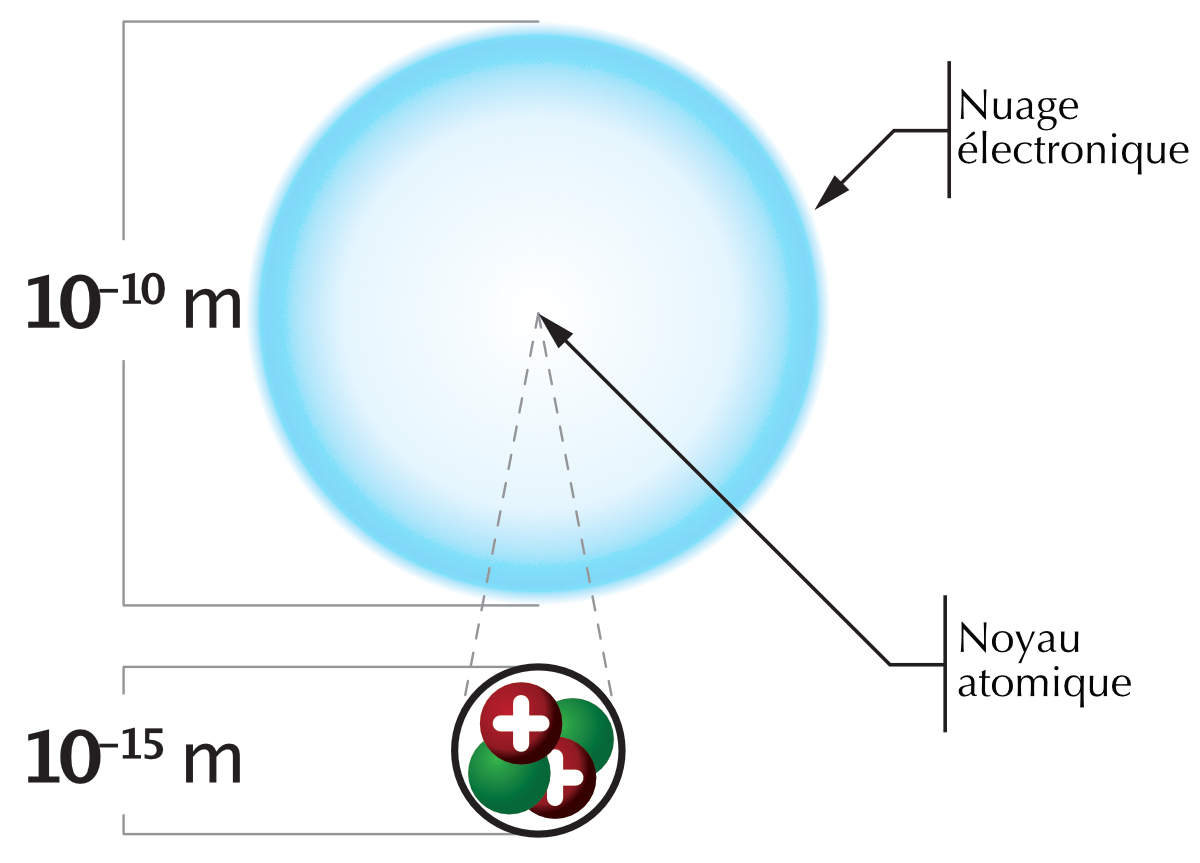
\includegraphics[width=0.33\linewidth]{images/ordre-grandeur-atome} 

}

\caption{Taille et structure de l'atome}\label{fig:ordre-grandeur-atome}
\end{figure}

\hypertarget{particules-subatomiques}{%
\section{Particules subatomiques}\label{particules-subatomiques}}

La matière est formée d'atomes et les atomes sont formés de particules subatomiques, les \textbf{protons}, les \textbf{neutrons} et les \textbf{électrons}.

Les mêmes particules subatomiques constituent tous les atomes. La seule chose qui varie d'un élément à l'autre est le nombre des particules subatomiques.

\begin{longtable}[]{@{}lccccc@{}}
\caption{\label{tab:particules-subatomiques} Les particules subatomiques.}\tabularnewline
\toprule
particule & symbole & charge {[}Coulomb{]} & charge relative & masse {[}kg{]} & masse relative\tabularnewline
\midrule
\endfirsthead
\toprule
particule & symbole & charge {[}Coulomb{]} & charge relative & masse {[}kg{]} & masse relative\tabularnewline
\midrule
\endhead
proton & \(p^{+}\) & \(+1.6\cdot10^{-19}\) & +1 & \(1.672\cdot10^{-27}\) & 1\tabularnewline
neutron & \(n^{}\) & 0 & 0 & \(1.674\cdot10^{-27}\) & \(\approx\) 1\tabularnewline
électron & \(e^{-}\) & \(-1.6\cdot10^{-19}\) & -1 & \(9.109\cdot10^{-31}\) & \(\frac{1}{1836}\)\tabularnewline
\bottomrule
\end{longtable}

Le proton porte une unité de charge positive, l'électron porte une unité de charge négative, et le neutron n'est pas chargé, il est électriquement neutre.

Un électron est 1836 fois plus léger qu'un proton, mais son influence est très grande car il porte une charge électrique équivalente à celle d'un proton.

\textbf{L'atome est électriquement neutre.} Comment un atome peut-il être neutre si il contient des protons chargés positivement et des électrons chargés négativement? La réponse est qu'\textbf{il y a un nombre égal de protons et d'électrons} de sorte que les charges positives et négatives s'annulent.

\begin{Exercise}

Le diamètre d'un atome de carbone est de 1.54 {[}angström{]} (1 {[}angström{]} = \(10^{-10}\) {[}m{]}).

\begin{enumerate}
\def\labelenumi{\arabic{enumi}.}
\tightlist
\item
  Exprimer ce diamètre en picomètres, en nanomètres.
  \vspace{\stretch{1}}
\item
  Combien d'atomes de carbone pourraient être alignés côte à côte sur la largeur d'un trait de crayon de 0.20 mm de large ?
  \vspace{\stretch{1}}
\end{enumerate}


\end{Exercise}

\begin{Answer}
1.54 {[}angström{]} = \(1.54\cdot10^{-10}\) {[}m{]}

\[ 1.54\cdot10^{-10} \text{ [m] } \cdot \frac{ 10^{12}\text{ [pm] }}{1\text{ [m] }} = 1.54\cdot10^{2} \text{ [pm] } = 154 \text{ [pm] } \]

\[ 1.54\cdot10^{-10} \text{ [m] } \cdot \frac{ 10^{9}\text{ [nm] }}{1\text{ [m] }} = 1.54\cdot10^{-1} \text{ [nm] } = 0.154 \text{ [nm] } \]

\[ \frac{0.2\cdot10^{-3} \text{ [m] }}{1.54\cdot10^{-10} \text{ [m/atome] }} = 1.3\cdot10^6 \text{ [atome] } \]

\end{Answer}

\begin{Exercise}

\begin{enumerate}
\def\labelenumi{\arabic{enumi}.}
\tightlist
\item
  Calculez, en gramme, la masse d'une molécule d'eau, en considérant que chaque atome d'hydrogène possède 1 proton et 1 électron (mais aucun neutron) et que le noyau d'un atome d'oxygène comporte 8 protons, 8 neutrons et 8 électrons.
  \vspace{\stretch{1}}
\item
  Combien y a-t-il de molécules d'eau dans 1 {[}ml{]} d'eau (1 {[}ml{]} d'eau = 1 {[}g{]} d'eau) ?
  \vspace{\stretch{1}}
\end{enumerate}


\end{Exercise}

\begin{Answer}
\[ \begin{split}
    m_{H} &= 1 \cdot m_{p} + 1 \cdot m_{e}\\
          &= 1.672\cdot10^{-27}\text{ [kg] } + 9.109\cdot10^{-31}\text{ [kg] }\\
          &= 1.672\cdot10^{-27}\text{ [kg] }\\
    m_{O} &= 8 \cdot m_{p} + 8 \cdot m_{n} + 8 \cdot m_{e}\\
          &= 8 \cdot 1.672\cdot10^{-27}\text{ [kg] } + 8 \cdot 1.674\cdot10^{-27}\text{ [kg] } + 8 \cdot 9.109\cdot10^{-31}\text{ [kg] }\\
          &= 2.678\cdot10^{-26}\text{ [kg] }\\
    m_{H_{2}O} &= 2 \cdot m_{H} + 1 \cdot m_{O}\\
          &= 2 \cdot 1.672\cdot10^{-27}\text{ [kg] } + 2.678\cdot10^{-26}\text{ [kg] }\\
          &= 3.012\cdot10^{-26}\text{ [kg] } = 3.012\cdot10^{-23} \text{ [g] pour une molécule}
\end{split} \]

1 {[}ml{]} d'eau = 1 {[}g{]} d'eau

\[ \begin{split}
    & \text{en utilisant la règle de trois : } \\
    1 \text{ molécule} &\rightarrow 3.012\cdot10^{-23} \text{ [g] }\\
    n \text{ molécules} &\rightarrow 1 \text{ [g] }\\
    n &= \frac{1}{3.012\cdot10^{-23}}\\
      &= 3.320\cdot10^{22} \text{ [molécules]}
\end{split}
\qquad
\begin{split}
    & \text{en utilisant une division simple : } \\
    n &= \frac{1\text{ [g] }}{ 3.012\cdot10^{-23} \text{ [g/molécule] } } \\
    &= 3.320\cdot10^{22} \text{ [molécules]}
\end{split} \]

\end{Answer}

\newpage

\hypertarget{les-uxe9luxe9ments}{%
\section{Les éléments}\label{les-uxe9luxe9ments}}

\begin{tcolorbox}
\textbf{Élément}\\
Un élément regroupe tous les atomes qui ont le même nombre de protons.

\end{tcolorbox}

On connaît actuellement 118 éléments différents. Ils sont classés dans le tableau périodique des éléments. Ce sont les briques de base de tous les \textbf{corps purs simples} et les \textbf{corps purs composés}.

Quelle est la différence entre deux atomes de deux éléments différents? Leur nombre de protons.

\begin{itemize}
\tightlist
\item
  Tous les atomes contenant \textbf{un proton} dans leur noyau sont des atomes d'\textbf{hydrogène}.
\item
  Tous les atomes contenant \textbf{deux protons} dans leur noyau sont des atomes d'\textbf{hélium}.
\item
  Tous les atomes contenant \textbf{trois protons} dans leur noyau sont des atomes de \textbf{lithium}.
\item
  \ldots{}
\end{itemize}

\hypertarget{les-symboles-et-les-noms}{%
\subsection{Les symboles et les noms}\label{les-symboles-et-les-noms}}

Dans le but de simplifier l'écriture, on représente les éléments chimiques par des symboles qui sont une lettre majuscule correspondant à l'initiale du nom de l'élément. Dans de nombreux cas, l'initiale seule ne suffit pas. On utilise alors une seconde lettre minuscule.

\begin{longtable}[]{@{}cll@{}}
\toprule
symbole & nom & origine\tabularnewline
\midrule
\endhead
H & hydrogène & qui forme de l'eau\tabularnewline
He & hélium & de Hélios, dieu grec du soleil\tabularnewline
Li & lithium & de Lithos, pierre en grec\tabularnewline
Be & béryllium & de béryl, un minerai\tabularnewline
B & bore & de borax, un minerai\tabularnewline
C & carbone & de Carbonis, charbon en grec\tabularnewline
N & azote & qui n'entretient pas la vie\tabularnewline
O & oxygène & qui forme des acides\tabularnewline
F & fluor & de fluere, s'écouler en latin\tabularnewline
Ne & néon & de Neos, nouveau en grec\tabularnewline
\bottomrule
\end{longtable}

Lorsque l'on représente un atome d'un élément chimique, il est souvent pratique également d'indiquer son numéro atomique \textbf{Z}. On écrit ce nombre en index en bas et à gauche du symbole.

\[ _{1}H \quad _{17}Cl \quad _{82}Pb \]

\newpage

\hypertarget{les-isotopes}{%
\section{Les isotopes}\label{les-isotopes}}

\begin{tcolorbox}
\textbf{Isotopes}\\
Atomes qui ont le même nombre de protons mais un nombre différent de neutrons.

\end{tcolorbox}

Les noyaux de tous les atomes contiennent des protons et des neutrons. Les neutrons qui accompagnent les protons d'un noyau rendent celui-ci plus ou moins lourd sans changer la charge de l'ensemble de l'atome. Le rôle des neutrons est d'assurer la stabilité du noyau atomique.

\textbf{Tous les atomes d'un même élément ont le même nombre de protons mais leur nombre de neutrons peut varier}. En effet, pour un même élément, il existe des atomes qui possèdent un nombre variable de neutrons.

Il existe des tables qui indiquent la liste des isotopes naturels stables et radioactifs pour chaque élément.

\begin{figure}

{\centering 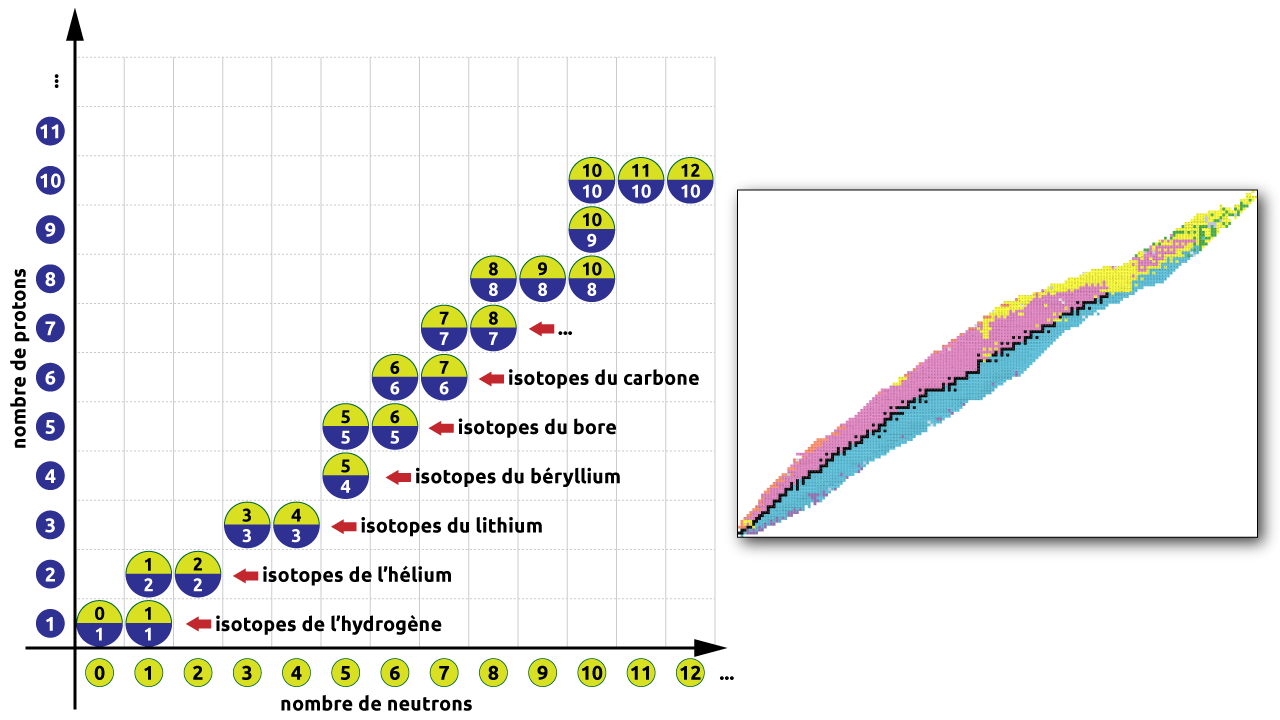
\includegraphics[width=0.8\linewidth]{images/isotopes-table} 

}

\caption{Table des isotopes simplifiée}\label{fig:isotopes-table}
\end{figure}

\begin{Exercise}
Dans les deux tableaux suivants, indiquez quelles espèces sont des isotopes d'un même élément. De quels éléments s'agit-il?

\end{Exercise}

\begin{longtable}[]{@{}cccc@{}}
\toprule
espèce & électrons & protons & neutrons\tabularnewline
\midrule
\endhead
A & 6 & 6 & 6\tabularnewline
B & 5 & 5 & 6\tabularnewline
C & 6 & 6 & 7\tabularnewline
D & 7 & 7 & 7\tabularnewline
E & 6 & 6 & 8\tabularnewline
\bottomrule
\end{longtable}

\begin{longtable}[]{@{}cccc@{}}
\toprule
espèce & électrons & protons & neutrons\tabularnewline
\midrule
\endhead
F & 7 & 7 & 6\tabularnewline
G & 6 & 6 & 6\tabularnewline
H & 9 & 9 & 7\tabularnewline
I & 7 & 7 & 7\tabularnewline
J & 7 & 7 & 8\tabularnewline
\bottomrule
\end{longtable}

\begin{Answer}

tableau 1 : A, C, E - 6 protons = Carbone.

tableau 2 : F, I, J - 7 protons = Azote.

\newpage


\end{Answer}

Dans la notation chimique, pour désigner un isotope, on indiquera le nombre de masse A de l'atome en exposant en haut et à gauche du symbol.

\[ \begin{split}
  _{Z}^{A}X
  \end{split}
  \qquad
  \begin{split}
  & \text{X : symbole de l'élément} \\
    & \text{A : nombre de masse de l'atome $\rightarrow$ protons + neutrons} \\
    & \text{Z : numéro atomique de l'élément $\rightarrow$ protons}
  \end{split} \]

\(_{6}^{12}C\) et \(_{6}^{13}C\) sont deux isotopes de l'élément carbone.On les nomme carbone 12 et carbone 13.

\(_{92}^{234}U\), \(_{92}^{235}U\) et \(_{92}^{238}U\) sont les isotopes naturels de l'élément uranium.

\begin{Exercise}
Complétez le tableau ci dessous pour chaque isotope considéré.

\end{Exercise}

\begin{longtable}[]{@{}cccccc@{}}
\toprule
symbole & A & protons & neutrons & électrons & nom de l'isotope\tabularnewline
\midrule
\endhead
\(_{6}^{14}C\) & & & & &\tabularnewline
\(_{3}^{7}Li\) & & & & &\tabularnewline
\(_{9}^{19}F\) & & & & &\tabularnewline
\bottomrule
\end{longtable}

\begin{Answer}
\(_{6}^{14}C\) : 14 / 6 / 8 / 6 / carbone 14

\(_{3}^{7}Li\) : 7 / 3 / 4 / 3 / lithium 7

\(_{9}^{19}F\) : 19 / 9 / 10 / 9 / fluor 19

\end{Answer}

\hypertarget{lunituxe9-de-masse-atomique}{%
\section{L'unité de masse atomique}\label{lunituxe9-de-masse-atomique}}

Les masses du protons et du neutrons sont d'environ \(1.672\cdot10^{-27}\) {[}kg{]} et la masse de l'électron est 1836 fois plus petite. Parce qu'il est peu pratique de travailler avec ces très petites masses exprimées en notation scientifique, les chimistes ont développé leur propre système de mesure de la masse d'un atome.

L'\textbf{unité de masse atomique (uma)} est une unité de mesure standard, utilisée pour mesurer la masse des atomes. Par convention, un atome de carbone 12, qui contient six protons et six neutrons a une masse de 12 {[}uma{]} exactement. Une unité de masse atomique est définie comme \(\frac{1}{12}\) de la masse cet atome.

\[ 1 [uma] \simeq 1,660 \cdot 10^{-27} [kg] \]

\begin{Exercise}
Calculez la masse du proton, du neutron et de l'électron en unité de masse atomique {[}uma{]}.

\end{Exercise}

\begin{longtable}[]{@{}ccc@{}}
\toprule
particule & masse en {[}kg{]} & masse en {[}uma{]}\tabularnewline
\midrule
\endhead
proton & \(1.672\cdot10^{-27}\) &\tabularnewline
neutron & \(1.674\cdot10^{-27}\) &\tabularnewline
électron & \(9.109\cdot10^{-31}\) &\tabularnewline
\bottomrule
\end{longtable}

\vspace{\stretch{1}}

\begin{Answer}

Exemple pour le proton :

\[ \begin{split}
  1~[uma] &\rightarrow 1,661\cdot10^{-27}~[kg] \\
  x~[uma] &\rightarrow 1,672\cdot10^{-27}~[kg] \\
  x &= \frac{1,672\cdot10^{-27}}{1,661\cdot10^{-27}} = 1.007
  \end{split} \]

\begin{itemize}
\tightlist
\item
  proton : 1.007
\item
  neutron : 1.008
\item
  électron : \(5.484\cdot10^{-4}\)
\end{itemize}


\end{Answer}

\hypertarget{le-duxe9faut-de-masse}{%
\subsection{Le défaut de masse}\label{le-duxe9faut-de-masse}}

On sait que des charges électriques semblables se repoussent entre-elles. Comment se fait-il que le noyau de l'atome, composé entre autres de protons chargé positivement, n'éclate-t-il pas sous l'effet des forces des répulsions électriques ? Ce sont les neutrons qui maintiennent la cohésion du noyau en exerçant une force d'attraction qui permet de lier fortement les nucléons (protons et neutrons) entre eux. Cette force est appelée \textbf{force nucléaire forte} et assure la stabilité du noyau atomique.

En mesurant la masse d'un noyau stable et en calculant la masse des nucléons qui forment ce noyau, on remarque que ces masses sont différentes. \textbf{La masse du noyau est plus petite que la somme des masses des nucléons}. C'est ce qu'on appelle \textbf{le défaut de masse}. Cette différence de masse est transformée en énergie de cohésion pour maintenir les nucléons ensemble. Maintenir un noyau stable n'est donc pas ``gratuit''.

Le défaut de masse est défini de la manière suivante :

\[
\Delta m = m_{\text{nucléons}} - m_{\text{noyau}}
\]

avec :

\begin{itemize}
\tightlist
\item
  \(\Delta m\) : défaut de masse en {[}uma{]}\\
\item
  \(m_{\text{nucléons}}\) : somme des masses des nucléons (\(m_p + m_n\)) en {[}uma{]}\\
\item
  \(m_{\text{noyau}}\) : masse mesurée du noyau en {[}uma{]}
\end{itemize}

\clearpage

Depuis le début du 20\textsuperscript{e} siècle, nous savons que, sous certaines conditions, une masse \(m\) peut se transformer en énergie \(E\), et vice versa. C'est le célèbre \(E = m \cdot c^2\) d'Albert Einstein.

\[
E = m \cdot c^2 \qquad \text{ou} \qquad \Delta E = \Delta m \cdot c^2 \qquad \text{donc} \qquad \Delta m = \frac{\Delta E}{c^2}
\]

avec :

\begin{itemize}
\tightlist
\item
  \(\Delta E\) : Énergie de cohésion en {[}J{]}\\
\item
  \(\Delta m\) : défaut de masse en {[}kg{]}\\
\item
  \(c\) : vitesse de la lumière en {[}m/s{]} (\(299\ 792\ 458\) {[}m/s{]} \(\approx 3 \cdot 10^8\) {[}m/s{]} )
\end{itemize}

\begin{Exercise}

\begin{enumerate}
\def\labelenumi{\arabic{enumi}.}
\tightlist
\item
  Quelle est la masse en kg d'un noyau d'hélium-4 ?\\
  \vspace{\stretch{1}}
\item
  La masse mesurée d'un noyau d'hélium-4 est de 4.002602 {[}uma{]}. Calculez la différence entre la masse mesurée et la masse obtenue par la somme des masses des particules subatomiques.
  \vspace{\stretch{1}}
\item
  Si il existe une différence, êtes-vous en mesure de l'expliquer ?
  \vspace{\stretch{1}}
\end{enumerate}


\end{Exercise}

\begin{Answer}

\begin{enumerate}
\def\labelenumi{\arabic{enumi}.}
\item
  \[
  \begin{split}
   m_{\text{calculée}} &= 2 \cdot m_{p+} + 2 \cdot m_{n} \\
   &= 2 \cdot 1.672 \cdot 10^{-27} \:[kg] + 2 \cdot 1.674 \cdot 10^{-27} \:[kg] \\
   &= 6.692 \cdot 10^{-27} \:[kg]
  \end{split}
  \]
\item
  \[   
  \begin{split}
   1\:[uma] &\rightarrow 1.660 \cdot 10^{-27} \:[kg] \\
   4.002602\:[uma] &\rightarrow x \:[kg]
  \end{split}
  \qquad
  \begin{split}
   m_{\text{mesurée}} &= 4.002602\:[uma] \cdot 1.660 \cdot 10^{-27} \:[kg/uma] \\
       &= 6.644 \cdot 10^{-27} \:[kg]
  \end{split}
  \]
  \[
  \begin{split}
   m_{\text{calculée}} - m_{\text{mesurée}} &= 6.692 \cdot 10^{-27} \:[kg] - 6.644 \cdot 10^{-27} \:[kg] \\
   &= 0.048 \cdot 10^{-27} \:[kg]
  \end{split}
  \]
\item
  La masse du noyau est inférieure à la somme des masses de chacun des protons et neutrons qui le composent. Une partie de la masse est donc transformée en énergie qui sert à la cohésion des particules du noyau.
\end{enumerate}

On peut faire le lien avec le célèbre \(E=m \cdot c^{2}\) exprimé par Albert Einstein (équivalence entre masse énergie).


\end{Answer}

\clearpage

\hypertarget{la-masse-atomique}{%
\section{La masse atomique}\label{la-masse-atomique}}

\begin{tcolorbox}
\textbf{Masse atomique}\\
La masse atomique d'un élément est la moyenne des masses de ses isotopes pondérée par leur abondance relative.

\end{tcolorbox}

La plupart des éléments sont présents dans la nature sous forme d'un mélange d'isotopes. On appelle \textbf{abondance isotopique} le pourcentage de chacun des isotopes présents dans l'élément considéré.

On peut déterminer la masse atomique d'un élément, en additionnant les masses de ses isotopes multipliées par leurs abondances relatives.

\begin{Exercise}
Calculer la masse atomique du chlore à l'aide des données suivantes :

\end{Exercise}

\begin{longtable}[]{@{}crr@{}}
\toprule
isotope & masse atomique & abondance\tabularnewline
\midrule
\endhead
\(_{17}^{35}Cl\) & 34.969 {[}uma{]} & 75.77\%\tabularnewline
\(_{17}^{37}Cl\) & 36.966 {[}uma{]} & 24.23\%\tabularnewline
\bottomrule
\end{longtable}

\vspace{\stretch{1}}

\begin{Answer}
\[ \begin{split}
    MA_{Cl} &=  MA_{Cl^{35}} \cdot Abd_{Cl^{35}} + MA_{Cl^{37}} \cdot Abd_{Cl^{37}}\\
        &= 34.969~[uma] \cdot 0.7577 + 36.966~[uma] \cdot 0.2423\\
        &= 35.45 [uma]
    \end{split} \]

\end{Answer}

\clearpage

\hypertarget{la-mole-et-le-nombre-davogadro}{%
\section{La mole et le nombre d'Avogadro}\label{la-mole-et-le-nombre-davogadro}}

Même les plus petits échantillons que nous traitons dans un laboratoire contiennent de gigantesques quantités d'atomes. Ne pouvant pas prendre les atomes, ou molécules, un par un avec des pincettes, les chimistes ont donc mis au point un système d'unité de comptage.

Dans la vie quotidienne, nous sommes familiers avec des unités de comptage comme la dizaine, la douzaine, la vingtaine, etc. En chimie, l'unité de comptage est la \textbf{mole}.

\begin{tcolorbox}
\textbf{La mole}\\
Une mole contient exactement \(6.02214076\cdot10^{23}\) entités élémentaires.

\end{tcolorbox}

Des techniques telles que la spectrométrie de masse, qui permettent de compter très précisément les atomes, ont été utilisées pour déterminer ce nombre. Ce nombre, noté \(N_A\), est appelé \textbf{nombre d'Avogadro} et dans le cadre de ce cours nous allons arrondir ce nombre à \(6.022\:\cdot\:10^{23}\).

\begin{longtable}[]{@{}ccl@{}}
\caption{\label{tab:unites-de-comptage} Unités de comptage.}\tabularnewline
\toprule
unité & nombre d'entités & exemple\tabularnewline
\midrule
\endfirsthead
\toprule
unité & nombre d'entités & exemple\tabularnewline
\midrule
\endhead
paire & 2 entités & une paire de chaussures\tabularnewline
dizaine & 10 entités & une dizaine de pommes\tabularnewline
douzaine & 12 entités & une douzaine d'oranges\tabularnewline
vingtaine & 20 entités & une vingtaine de personnes\tabularnewline
mole & \(6.022\cdot10^{23}\) entités & une mole d'atomes de potassium\tabularnewline
\bottomrule
\end{longtable}

Une mole d'atomes, une mole de molécules, ou une mole de quoi que ce soit contiennent toutes \(6.022\cdot10^{23}\) objets.

\begin{Exercise}

De par la définition de l'unité de masse atomique, un seul atome de carbone 12 a une masse de 12 {[}uma{]}. Calculez la masse en grammes d'une mole d'atomes de carbone 12.

\vspace{\stretch{1}}


\end{Exercise}

\begin{Answer}
\[ \begin{split}
    \text{1 atome de } ^{12}C &\\
    1 [uma] &\longrightarrow 1.661\cdot10^{-24} [g]\\
    12 [uma] &\longrightarrow m [g]
    \end{split}
    \qquad\qquad
    \begin{split}
        m &= \dfrac{12 [uma] \cdot 1.661 \cdot 10^{-24} [g]}{1 [uma]}\\
        &= 1.9932\cdot 10^{-23} [g]     
    \end{split} \]

\[ \begin{split}
        \text{1 mole d'atomes de }^{12}C &\\
        \text{1 [atome] de }^{12}C &\longrightarrow 1.9932\cdot 10^{-23} [g]\\
        \quad 6.022\cdot 10^{23} [atome] &\longrightarrow M [g]\\
    \end{split}
    \qquad\qquad
    \begin{split}
    M &= \dfrac{6.022\cdot 10^{23} \cdot 1.9932\cdot 10^{-23} [g]}{1 [atome]}\\
    &= 12 [g]
    \end{split} \]

Une mole d'atomes de carbone 12 a une masse de 12 {[}g{]}.

\end{Answer}

\begin{Exercise}

Un seul atome d'oxygène 16 a une masse de 15,9949 {[}uma{]}. Calculez la masse en grammes d'une mole d'atomes d'oxygène 16.

\vspace{\stretch{1}}


\end{Exercise}

\begin{Answer}
\[ \begin{split}
    \text{1 atome de }^{16}O &\\
    1 [uma] &\longrightarrow 1.661\cdot10^{-24} [g]\\
    16 [uma] &\longrightarrow m [g]\\
    \end{split}
    \qquad\qquad
    \begin{split}
        m &= \dfrac{16 [uma] \cdot 1.661 \cdot 10^{-24} [g]}{1 [uma]}\\
        &= 2.657\cdot 10^{-23} [g]
    \end{split} \]

\[ \begin{split}
    \text{1 mole d'atomes de }^{16}O &\\
    \text{1 [atome] de } ^{16}O &\longrightarrow 2.657\cdot 10^{-23} [g]\\
    6.022\cdot 10^{23} [atome] &\longrightarrow M [g]\\
    \end{split}
    \qquad\qquad
    \begin{split}
    M &= \dfrac{6.022\cdot 10^{23} \cdot 2.657\cdot 10^{-23} [g]}{1 [atome]}\\
    &= 16 [g]
    \end{split} \]

Une mole d'atomes d'oxygène 16 a une masse de 16 {[}g{]}.

\end{Answer}

\clearpage

\begin{Exercise}

Sur la base des résultats des deux exercices ci-dessus, identifiez la relation entre les valeurs numériques de la masse d'un atome en {[}uma{]} et la masse d'une mole d'atomes en {[}g/mol{]}.

\vspace{\stretch{1}}


\end{Exercise}

\begin{Answer}
La masse en grammes par mole d'une substance est numériquement égale à son poids en unités de masse atomique.

\[ \underbrace{\{masse\;atomique\}}_\text{[uma]}\;=\;\underbrace{\{masse\;molaire\}}_\text{[g/mol]} \]

\end{Answer}

\hypertarget{la-masse-molaire-atomique}{%
\section{La masse molaire atomique}\label{la-masse-molaire-atomique}}

\begin{figure}

{\centering 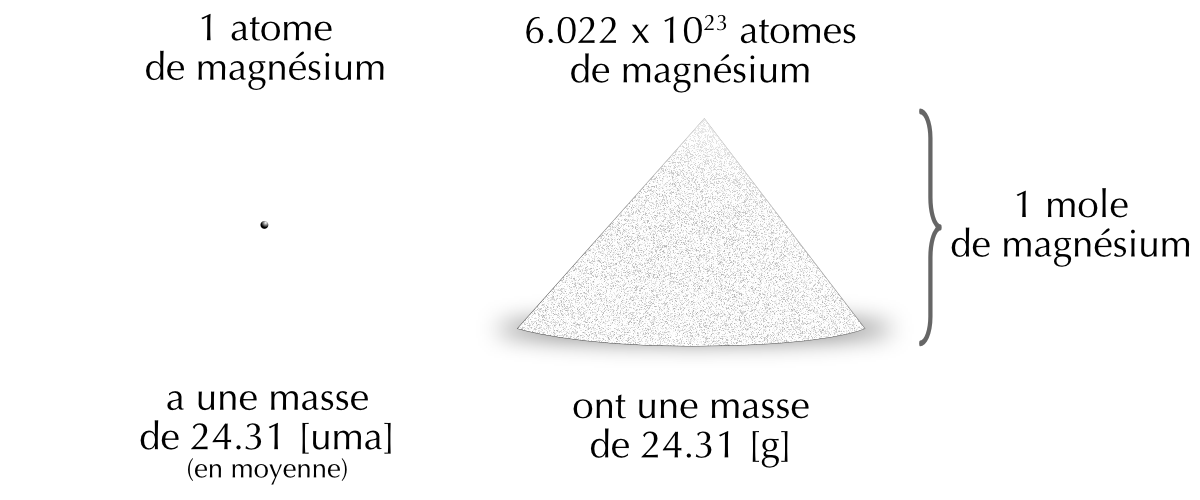
\includegraphics[width=0.67\linewidth]{images/uma-masse-molaire} 

}

\caption{Relation entre unité de masse atomique et masse molaire.}\label{fig:uma-masse-molaire}
\end{figure}

\begin{tcolorbox}
\textbf{Masse molaire atomique}\\
La masse molaire atomique d'un élément est la masse en grammes d'une mole d'atomes de l'élément.

\end{tcolorbox}

La définition de la masse molaire nous permet d'exprimer la relation suivante:

\[ \begin{split}
  \text{M} = \frac{\text{m}}{\text{n}}
\end{split}
\qquad
\begin{split}
    &\text{m : masse de substance en [g]}\\
    &\text{n : quantité de matière en [mol]}\\
    &\text{M : masse molaire en [g/mol]}
\end{split} \]

\[ M = \frac{m}{n} \qquad \text{ ou } \qquad n = \frac{m}{M} \qquad \text{ ou } \qquad m = n \cdot M \]

\begin{Exercise}
Complétez le tableau ci dessous, indiquant la masse molaire du composé en {[}g/mol{]} et le nombre de moles contenues dans 1{[}g{]} de cet élément.

\end{Exercise}

\begin{longtable}[]{@{}ccc@{}}
\toprule
substance & masse molaire en {[}g/mol{]} & moles contenues dans 1{[}g{]}\tabularnewline
\midrule
\endhead
Fe & &\tabularnewline
Pb & &\tabularnewline
Mg & &\tabularnewline
\bottomrule
\end{longtable}

\begin{Answer}
Fe - 55.85 {[}g/mol{]} - 1{[}g{]} / 55.85{[}g/mol{]} = 0.018 {[}mol{]}

Pb - 207.2 {[}g/mol{]} - 1{[}g{]} / 207.2{[}g/mol{]} = 0.005 {[}mol{]}

Mg - 24.31 {[}g/mol{]} - 1{[}g{]} / 24.31{[}g/mol{]} = 0.041 {[}mol{]}

\end{Answer}

\clearpage

\hypertarget{exercices-suppluxe9mentaires-3}{%
\section{Exercices supplémentaires}\label{exercices-suppluxe9mentaires-3}}

\begin{Exercise}

Combien de protons, de neutrons et d'électrons sont contenus dans un atome de:

\begin{enumerate}
\def\labelenumi{\arabic{enumi}.}
\tightlist
\item
  \(^{197}\text{Au}\)\\
  \vspace{\stretch{1}}
\item
  strontium 90\\
  \vspace{\stretch{1}}
\end{enumerate}


\end{Exercise}

\begin{Answer}

\begin{enumerate}
\def\labelenumi{\arabic{enumi}.}
\tightlist
\item
  Z de l'or = 79\\
  Un atome de \(^{197}Au\) a 79 protons, 79 électrons, et 197-79 = 118 neutrons.\\
\item
  Z du strontium = 38\\
  L'isotope strontium 90 a 38 protons, 38 électrons et 90-38 = 52 neutrons.
\end{enumerate}


\end{Answer}

\begin{Exercise}

Le magnésium a trois isotopes dont les nombres de masse sont 24, 25 et 26.

\begin{enumerate}
\def\labelenumi{\arabic{enumi}.}
\tightlist
\item
  Donnez le symbole chimique complet (exposant et indice) pour chaque isotope.\\
  \vspace{\stretch{1}}
\item
  Combien de neutrons sont contenus dans un atome de chaque isotope ?\\
  \vspace{\stretch{1}}
\end{enumerate}


\end{Exercise}

\begin{Answer}

\begin{enumerate}
\def\labelenumi{\arabic{enumi}.}
\tightlist
\item
  \(_{12}^{24}Mg\), \(_{12}^{25}Mg\) et \(_{12}^{26}Mg\)\\
\item
  12 neutrons, 13 neutrons et 14 neutrons
\end{enumerate}


\end{Answer}

\begin{Exercise}
Complétez le tableau suivant pour retrouver l'isotope considéré à chaque ligne.

\end{Exercise}

\begin{longtable}[]{@{}ccccc@{}}
\toprule
symbole & A & protons & neutrons & nom de l'isotope\tabularnewline
\midrule
\endhead
& & 7 & 6 &\tabularnewline
& 16 & 8 & &\tabularnewline
& 17 & & 9 &\tabularnewline
& 15 & & 8 &\tabularnewline
\bottomrule
\end{longtable}

\begin{Answer}

\(_{7}^{13}N\) \textbar{} 13 \textbar{} 7 \textbar{} 6 \textbar{} azote 13

\(_{8}^{16}O\) \textbar{} 16 \textbar{} 8 \textbar{} 8 \textbar{} oxygène 16

\(_{8}^{17}O\) \textbar{} 17 \textbar{} 8 \textbar{} 9 \textbar{} oxygène 17

\(_{7}^{15}N\) \textbar{} 15 \textbar{} 7 \textbar{} 8 \textbar{} azote 15

\newpage


\end{Answer}

\begin{Exercise}

Donnez le symbole chimique complet de l'atome dont le nombre de masse est de 112 et le numéro atomique égal à 48.

\vspace{\stretch{1}}

Donnez le nombre de chacune des particules qui le composent.

\vspace{\stretch{1}}


\end{Exercise}

\begin{Answer}
\(_{48}^{112}Cd\)

48 protons, 64 neutrons et 48 électrons

\end{Answer}

\begin{Exercise}

Soit un atome de sodium 23. Qu'obtiendrait-on \ldots{}

\begin{enumerate}
\def\labelenumi{\arabic{enumi}.}
\tightlist
\item
  si on pouvait lui ajouter un proton ?\\
  \vspace{\stretch{1}}
\item
  si on pouvait lui ajouter un neutron ?\\
  \vspace{\stretch{1}}
\end{enumerate}


\end{Exercise}

\begin{Answer}

\begin{enumerate}
\def\labelenumi{\arabic{enumi}.}
\tightlist
\item
  du magnésium 24.
\item
  un autre isotope du sodium
\end{enumerate}


\end{Answer}

\newpage

\begin{Exercise}

Chacun des symboles chimiques ci-dessous représente un élément différent. Identifiez l'élément représenté et donnez le nombre de protons, de neutrons et d'électrons de chacun:

\begin{enumerate}
\def\labelenumi{\arabic{enumi}.}
\tightlist
\item
  \(^{74}_{33}X\)\\
\item
  \(^{127}_{53}X\)\\
\item
  \(^{152}_{63}X\)\\
\item
  \(^{209}_{83}X\)
\end{enumerate}


\end{Exercise}

\begin{Answer}

\begin{enumerate}
\def\labelenumi{\arabic{enumi}.}
\tightlist
\item
  \(^{74}_{33}As\) : 33 \(p^+\), 41 \(n\), 33 \(e^-\)\\
\item
  \(^{127}_{53}I\) : 53 \(p^+\), 74 \(n\), 53 \(e^-\)\\
\item
  \(^{152}_{63}Eu\) : 63 \(p^+\), 89 \(n\), 63 \(e^-\)\\
\item
  \(^{209}_{83}Bi\) : 83 \(p^+\), 126 \(n\), 83 \(e^-\)
\end{enumerate}


\end{Answer}

\begin{Exercise}

Quelle serait la masse atomique d'un l'élément si cet élément était composé de trois isotopes avec les abondances relatives suivantes?

\begin{itemize}
\tightlist
\item
  30.00 \% à 37.00 {[}uma{]}
\item
  50.00 \% à 38.00 {[}uma{]}
\item
  20.00 \% à 40.00 {[}uma{]}
\end{itemize}

\vspace{\stretch{1}}


\end{Exercise}

\begin{Answer}
\[ \begin{split}
        m_a & = 0.3 \cdot 37.00 [uma] + 0.5 \cdot 38.00 [uma] + 0.2 \cdot 40.00 [uma]\\
        &= 38.1 [uma]
\end{split} \]

\end{Answer}

\begin{Exercise}

Vous portez à votre doigt un anneau d'or pur qui pèse 31,6 {[}g{]}.

\begin{enumerate}
\def\labelenumi{\arabic{enumi}.}
\tightlist
\item
  Combien de moles d'atomes d'or sont contenues dans cet anneau?\\
  \vspace{\stretch{1}}
\item
  Combien d'atomes d'or sont contenus dans cet anneau?\\
  \vspace{\stretch{1}}
\item
  Combien de protons sont contenus dans cet anneau?\\
  \vspace{\stretch{1}}
\end{enumerate}


\end{Exercise}

\begin{Answer}
\[ \begin{split}
    1 [mol] \text{ d 'Au } &\longrightarrow 196.97 [g]\\
    n [mol] \text{ d 'Au } &\longrightarrow 31.6 [g]\\
    n &= \dfrac{31.6 [g] \cdot 1 [mol]}{196.97 [g]} = 0.16 [mol]
\end{split} \]

\textbf{31.6 {[}g{]} d'or contiennent 0.16 {[}mol{]} d'atomes d'or.}

\[ \begin{split}
    1 [mol] \text{ d'Au } &\longrightarrow 6.022\cdot 10^{23} [atome] \text{ d'Au}\\
    0.16 [mol] \text{ d'Au } &\longrightarrow N_a [atome] \text{ d'Au}\\
    N_a = \dfrac{0.16 [mol] \cdot 6.022\cdot 10^{23} [atome]}{1 [mol]} &= 9.66\cdot 10^{22} [atome]
\end{split} \]

\textbf{31.6 {[}g{]} d'or contiennent \(9.66\cdot 10^{22}\) atomes d'or.}

\[ \begin{split}
    1 [atome] \text{ d'Au } &\longrightarrow 79 [proton]\\
    9.66\cdot 10^{22} [atome] \text{ d'Au } &\longrightarrow N_{p} [proton]\\
    N_p = \dfrac{9.66\cdot 10^{22} [atome] \cdot 79 [proton]}{1 [atome]} &= 7.63\cdot 10^{24} [proton]\\
\end{split} \]

\textbf{31.6 {[}g{]} d'or contiennent \(7.63\cdot 10^{24}\) protons.}

\end{Answer}

\newpage

\begin{Exercise}

Calculer le nombre d'atomes de magnésium contenus dans 35.2 g de magnésium.

\vspace{\stretch{1}}

Quelle est la masse de 2.2 \(\cdot 10^{23}\) atomes de Pt?

\vspace{\stretch{1}}

Combien de grammes de calcium (Ca) faut-il pour obtenir 3.40 moles de calcium?

\vspace{\stretch{1}}


\end{Exercise}

\begin{Answer}

\begin{enumerate}
\def\labelenumi{\arabic{enumi}.}
\item
  \[ \begin{split}
       n &= \dfrac{m}{M} = \dfrac{35.2~[g]}{24.31~[g/mol]} = 1.45~[mol] \\
       N &= n \cdot N_{A} = 1.45~[mol] \cdot 6.022\cdot10^{23} = 8.73\cdot10^{23}~[atomes]
       \end{split} \]
\item
  \[ \begin{split}
       n &= \dfrac{N}{N_{A}} = \dfrac{2.2\cdot10^{23}}{6.022\cdot10^{23}} = 0.37~[mol] \\
       m &= n \cdot M = 0.37[mol] \cdot 195.08[g/mol] = 72[g]
       \end{split} \]
\item
  \[ \begin{split}
       m &= n \cdot M = 3.4[mol] \cdot 40.08[g/mol] = 136[g]
       \end{split} \]
\end{enumerate}


\end{Answer}

\begin{Exercise}

Combien de mole d'atomes de carbone contiennent 6 {[}g{]} de carbone 12?

\vspace{\stretch{1}}

Combien d'atomes sont contenus dans 97.6 {[}g{]} de platine?

\vspace{\stretch{1}}

Combien d'atomes contient un échantillon de chrome ayant une masse de 13 {[}g{]}?

\vspace{\stretch{1}}

Combien de moles d'argent représentent 9.02 \(\cdot 10^{23}\) molécules d'argent?

\vspace{\stretch{1}}


\end{Exercise}

\begin{Answer}

\begin{enumerate}
\def\labelenumi{\arabic{enumi}.}
\item
  \[ \begin{split}
           1 \text{ [mol] de C } &\longrightarrow 12 [g]\\
           n \text{ [mol] de C } &\longrightarrow 6 [g]\\
           n = \dfrac{6 [g] \cdot 1 [mol]}{12 [g]} &= 0.5 [mol]
       \end{split}
       \qquad
       \begin{split}
       n = \dfrac{m}{M} = \dfrac{6[g]}{12[g/mol]} = 0.5 [mol]
   \end{split} \]
\item
  \[ \begin{split}
           1 \text{ [mol] de Pt } &\longrightarrow 195 [g]\\
           n \text{ [mol] de Pt } &\longrightarrow 97.6 [g]\\
           n = \dfrac{97.6 [g] \cdot 1 [mol]}{195 [g]} &= 0.5 [mol]
       \end{split}
       \qquad
       \begin{split}
       n = \dfrac{m}{M} = \dfrac{97.6[g]}{195[g/mol]} = 0.5 [mol]
   \end{split} \]
\end{enumerate}

\[ \begin{split}
  1 \text{ [mol] de Pt } &\longrightarrow 6.022^\cdot10^{23} [atome]\\
  0.5 \text{ [mol] de Pt } &\longrightarrow n [atome]\\
  n = \dfrac{0.5 [mol] \cdot 6.022^\cdot10^{23} [atome]}{1 [mol]} &= 3.011^\cdot10^{23} [atome]
  \end{split} \]

\begin{enumerate}
\def\labelenumi{\arabic{enumi}.}
\setcounter{enumi}{2}
\tightlist
\item
  \[ \begin{split}
       1 \text{ [mol] de Cr } &\longrightarrow 52 [g]\\
       n \text{ [mol] de Cr } &\longrightarrow 13 [g]\\
       n = \dfrac{13 [g] \cdot 1 [mol]}{52 [g]} &= 0.25 [mol]
       \end{split}
       \qquad
       \begin{split}
       n = \dfrac{m}{M} = \dfrac{13[g]}{52[g/mol]} &= 0.25 [mol]
   \end{split} \]
\end{enumerate}

\[ \begin{split}
  1 \text{ [mol] de Cr } &\longrightarrow 6.022^\cdot10^{23} [atome]\\
  0.25 \text{ [mol] de Cr } &\longrightarrow n [atome]\\
  n = \dfrac{0.25 [mol] \cdot 6.022^\cdot10^{23} [atome]}{1 [mol]} &= 1.51^\cdot10^{23} [atome]
  \end{split} \]

\begin{enumerate}
\def\labelenumi{\arabic{enumi}.}
\setcounter{enumi}{3}
\tightlist
\item
  \[ \begin{split}
       1 \text{ [mol] de Ag } &\longrightarrow 6.022^\cdot10^{23} [molecule]\\
       n \text{ [mol] de Ag } &\longrightarrow 9.02^\cdot10^{23} [molecule]\\
       n &= \dfrac{9.02^\cdot10^{23} [molecule] \cdot 1[mol]}{6.022^\cdot10^{23} [molecule]} = 1.51 [mol]
   \end{split} \]
\end{enumerate}


\end{Answer}

\newpage

\section{Solutions des exercices} \shipoutAnswer

\hypertarget{le-tableau-puxe9riodique}{%
\chapter{Le tableau périodique}\label{le-tableau-puxe9riodique}}

\begin{objectives}

\begin{itemize}
\tightlist
\item
  Décrire comment les éléments sont organisés dans le tableau périodique donnant lieu à des périodes et des groupes.
\item
  Décrire les caractéristiques ondulatoires de la lumière (fréquence, la longueur d'onde et énergie) et les régions générales du spectre électromagnétique.
\item
  Décrire comment la matière interagit avec les rayonnements électromagnétiques et mène aux spectres d'absorption et d'émission.
\item
  Repérer les éléments sur le tableau périodique et les classer en métaux, non-métaux ou métalloïdes.
\item
  Décrire la répartition des électrons en couches, sous-couches et orbitales autour du noyau atomique.
\item
  Prédire la structure électronique d'un élément grâce au tableau périodique.
\item
  Identifier les électrons de valence d'un atome et leurs correspondance avec les différents groupes du tableau périodique.
\item
  Représenter la structure de Lewis d'un atome donné.
\item
  Définir les termes ions, cations et anions.
\item
  Utiliser la régle de l'octet pour prédire l'ion stable que formera un élément du bloc principal.
\end{itemize}


\end{objectives}

A la fin du 18ème siècle, Lavoisier a compilé une liste des 23 éléments connus à l'époque. En 1870, on en connaissait 65, et 88 en 1925. Aujourd'hui, on en dénombre 118.

Les chimistes ont regroupé les éléments de sorte à ce qu'ils n'aient pas à mémoriser individuellement les propriétés de chaque élément. Dans leurs tentatives de classification, plusieurs chercheurs ont remarqué des récurrences, ou périodes, dans leur classification.

\hypertarget{la-classification-puxe9riodique}{%
\section{La classification périodique}\label{la-classification-puxe9riodique}}

En 1871, le chimiste russe \textbf{Dmitri Mendeleev} (1836-1907) a présenté le premier \textbf{tableau périodique}. Il a classé les éléments par masse atomique croissante et il a ensuite organisé les éléments avec des propriétés chimiques similaires dans la même colonne.

Plus tard, le tableau périodique moderne a été introduit. Il classe les éléments par numéro atomique et non par masse atomique, mais le principe est le même que le classement de Mendeleev.

\clearpage

Chaque case du tableau représente un élément différent et contient au moins trois informations:

\begin{itemize}
\tightlist
\item
  le symbole de l'élément
\item
  le numéro atomique de l'élément
\item
  la masse atomique de l'élément
\end{itemize}

\begin{figure}

{\centering 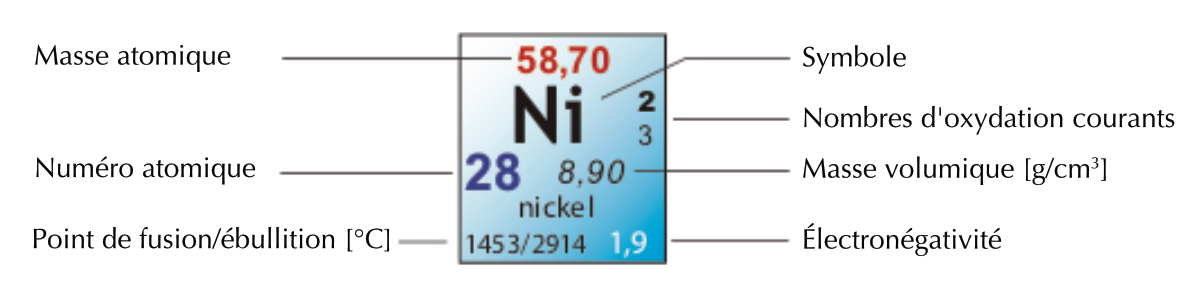
\includegraphics[width=0.67\linewidth]{images/tpe-case} 

}

\caption{Une case du tableau périodique}\label{fig:tpe-case}
\end{figure}

Le tableau périodique contient souvent des informations supplémentaires sur les éléments, il peut contenir des couleurs différentes ou il peut être écrit dans différentes langues, mais la structure de base du tableau reste la même.

\hypertarget{muxe9taux-non-muxe9taux-muxe9tallouxefdes}{%
\subsection{Métaux, non-métaux, métalloïdes}\label{muxe9taux-non-muxe9taux-muxe9tallouxefdes}}

Si aujourd'hui, 86 métaux sont présents dans le tableau de Mendeleïev, seuls sept d'entre eux étaient connus et isolés jusqu'au Moyen Age :

\begin{longtable}[]{@{}ll@{}}
\toprule
élément & découverte\tabularnewline
\midrule
\endhead
or & 6000 av. J.-C.\tabularnewline
cuivre & 4000 av. J.-C.\tabularnewline
argent & 3500 av. J.-C.\tabularnewline
plomb & 3500 av. J.-C.\tabularnewline
étain & 3000 av. J.-C.\tabularnewline
fer & 1500 av. J.-C.\tabularnewline
mercure & 750 av. J.-C.\tabularnewline
\bottomrule
\end{longtable}

Les \textbf{métaux} sont solides à température et pression ambiante, à l'exception du mercure qui est liquide. Ils ont une apparence brillante et sont de bons conducteurs de la chaleur et de l'électricité. Ils sont malléables et ductiles.

Les éléments B, Si, Ge, As, Sb, Te, Po et At sont appelés \textbf{métalloïdes}. Les métalloïdes ont les propriétés des métaux et des non-métaux. Leurs propriétés électriques inhabituelles sont employée dans l'industrie des semi-conducteurs et en fabrication informatique.

Le reste des éléments, à droite des métalloïdes, sont appelés \textbf{non-métaux}. Les non-métaux ont des propriétés qui sont souvent opposées à celles des métaux. Certains sont des gaz, ils sont de mauvais conducteurs de la chaleur et de l'électricité, ils ne sont ni malléables, ni ductiles.

\begin{figure}

{\centering 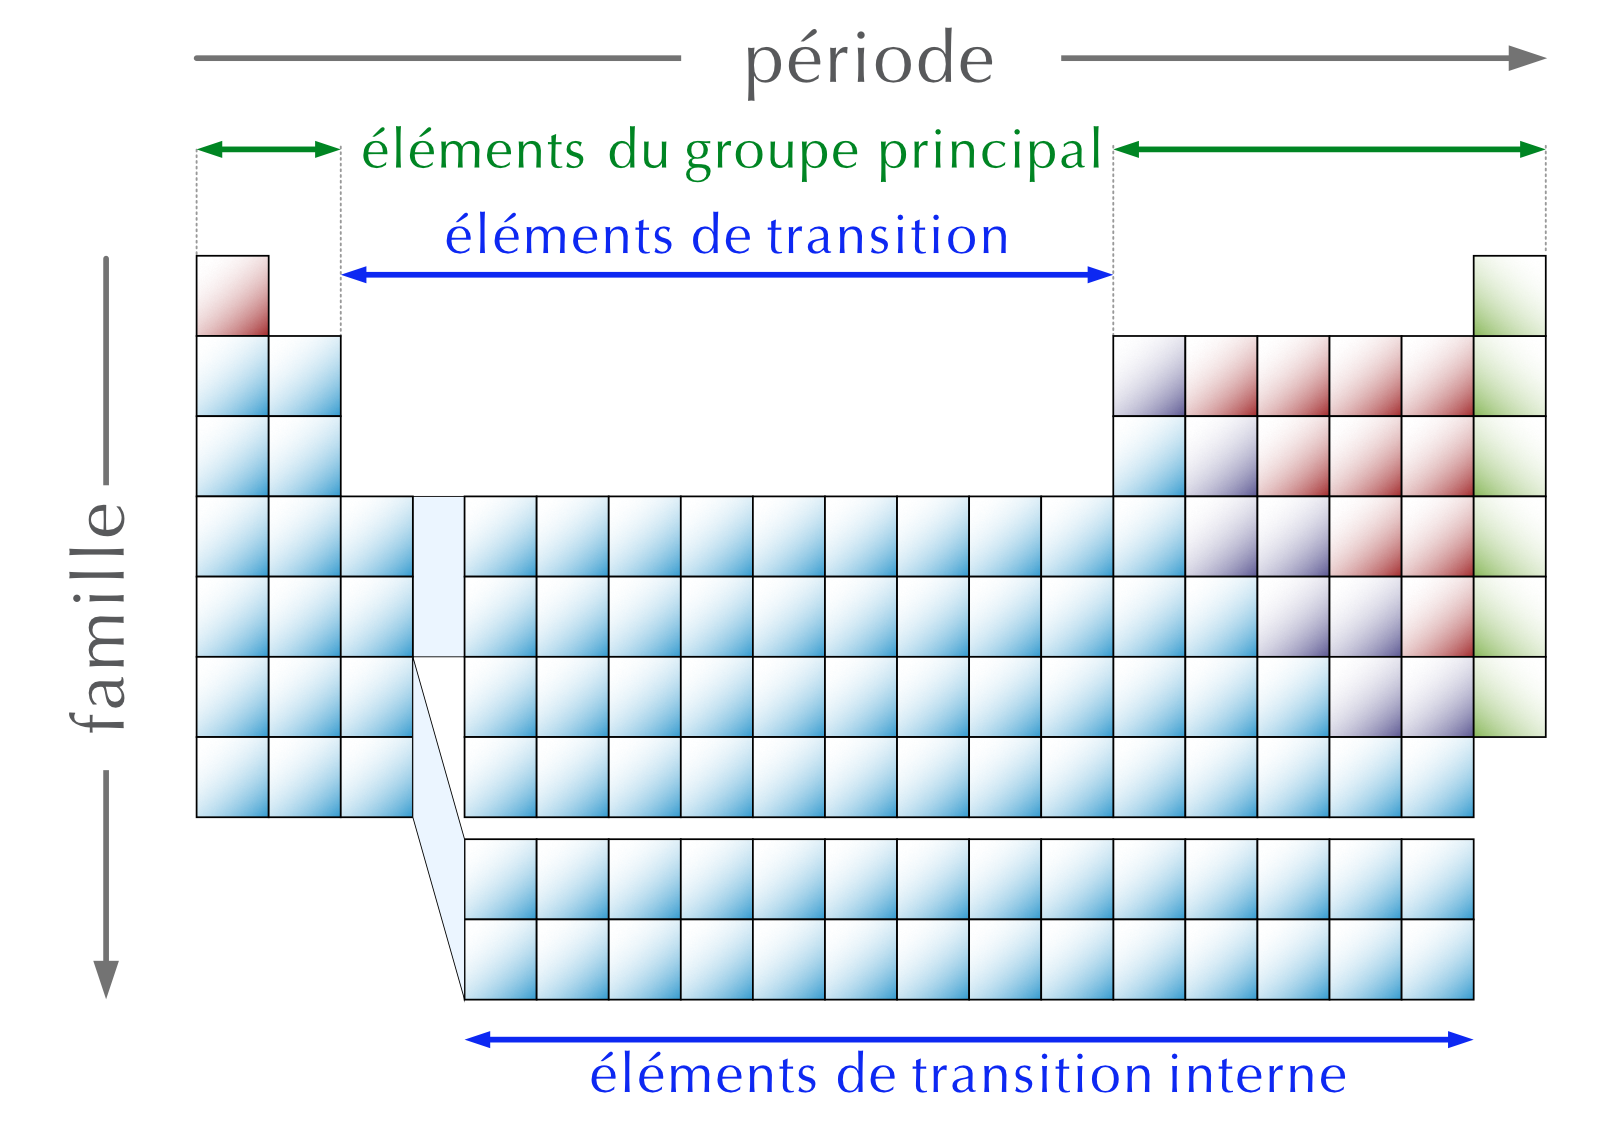
\includegraphics[width=0.45\linewidth]{images/tpe-empty} 

}

\caption{Le vocabulaire du tableau périodique}\label{fig:tpe-empty}
\end{figure}

\hypertarget{les-puxe9riodes}{%
\subsection{Les périodes}\label{les-puxe9riodes}}

Les \textbf{lignes} du tableau périodique sont appelées \textbf{périodes} et chacune est désignée par un nombre de 1 à 7 (première période, deuxième période, etc.). Le nom de tableau périodique provient du fait que les propriétés reviennent périodiquement à chaque fois qu'on change de ligne.

Le tableau périodique regroupe les éléments par période, mais les propriétés chimiques des éléments d'une même période sont différentes. Le classement par période représente l'arrangement des électrons au sein des éléments.

\hypertarget{les-familles}{%
\subsection{Les familles}\label{les-familles}}

Les \textbf{colonnes} du tableau périodique sont appelées \textbf{familles}. Le tableau périodique classe les éléments de sorte que les éléments ayant des propriétés chimiques similaires apparaissent dans la même colonne formant ainsi une famille d'éléments.

Il y a au total 18 familles et il existe différentes manières de les numéroter. Dans votre tableau périodique, les familles du \textbf{groupe principal} sont désignées avec un chiffre romain de I à VIII. Vous verrez peut-être d'autres numérotations, l'Union Internationale de Chimie Pure et Appliquée (UICPA) a décidé que le système officiel de numérotation des groupes serait de 1 à 18, de gauche à droite. De nombreux tableaux périodiques présentent plusieurs systèmes simultanément.

\begin{longtable}[]{@{}cll@{}}
\caption{\label{tab:noms-groupes-courants} Noms de quelques groupes couramment employés.}\tabularnewline
\toprule
Groupe & nom & éléments\tabularnewline
\midrule
\endfirsthead
\toprule
Groupe & nom & éléments\tabularnewline
\midrule
\endhead
I & métaux alcalins & Li, Na, K, Rb, Cs, Fr\tabularnewline
II & métaux alcalino-terreux & Be, Mg, Ca, Sr, Ba, Ra\tabularnewline
VI & chalcogènes & O, S, Se, Te, Po\tabularnewline
VII & halogènes & F, Cl, Br, I, At\tabularnewline
VIII & les gaz rares (ou gaz nobles) & He, Ne, Ar, Kr, Xe, Rn\tabularnewline
\bottomrule
\end{longtable}

Les \textbf{éléments de transition internes} ont été décalés dans le tableau périodique afin de rendre ce dernier plus compact.

\hypertarget{interactions-rayonnement-matiuxe8re}{%
\section{Interactions rayonnement-matière}\label{interactions-rayonnement-matiuxe8re}}

Une onde est une perturbation de l'état physique d'un milieu qui se propage. Elle transporte de l'énergie sans transporter de matière. Par exemple, lorsqu'on lance un caillou dans l'eau, la surface de l'eau est modifiée et des vagues apparaissent à sa surface; lorsque l'on frappe dans ses mains, cette variation de pression de propage dans l'air ambiant; quand on frotte une corde de violon avec un archet, on peut voir la corde vibrer et l'entendre grâce à la propagation de la vibration dans l'air.

Les objets quantiques, comme la lumière et les électrons, ont la particularité de se comporter \textbf{à la fois} comme des ondes ou des particules. Un électron a, par exemple, une masse et une charge électrique. Il peut être défini comme une particule. Alors que si on laisse cet électron se déplacer librement sans l'observer, il aura les caractéristiques d'une onde. Pour expliquer la structure et le comportement des atomes, il est nécessaire de considérer que les particules ont des propriétés ondulatoires.

\hypertarget{les-ondes-uxe9lectromagnuxe9tiques}{%
\subsection{Les ondes électromagnétiques}\label{les-ondes-uxe9lectromagnuxe9tiques}}

Les ondes qui vont nous intéresser pour décrire les électrons sont les \textbf{ondes électromagnétiques}. Une onde électromagnétique est une perturbation du champ électromagnétique qui se propage. Elle a la particularité de se propager aussi bien dans un milieu matériel que dans le vide. Les ondes radio, les ondes lumineuses ou les rayons X sont des exemples d'onde électromagnétique.

\hypertarget{longueur-donde-fruxe9quence-et-vitesse}{%
\subsection{Longueur d'onde, fréquence et vitesse}\label{longueur-donde-fruxe9quence-et-vitesse}}

Si on dessine un faisceau lumineux sous la forme d'une onde, nous appellerons \textbf{longueur d'onde}, la distance entre deux crêtes (ou entre deux creux ou entre deux positions identiques sur l'onde). Si on considère que cette onde se déplace de gauche à droite et si on compte le nombre de crêtes qui passent par un point particulier chaque seconde, on obtient la \textbf{fréquence}.

\begin{figure}

{\centering 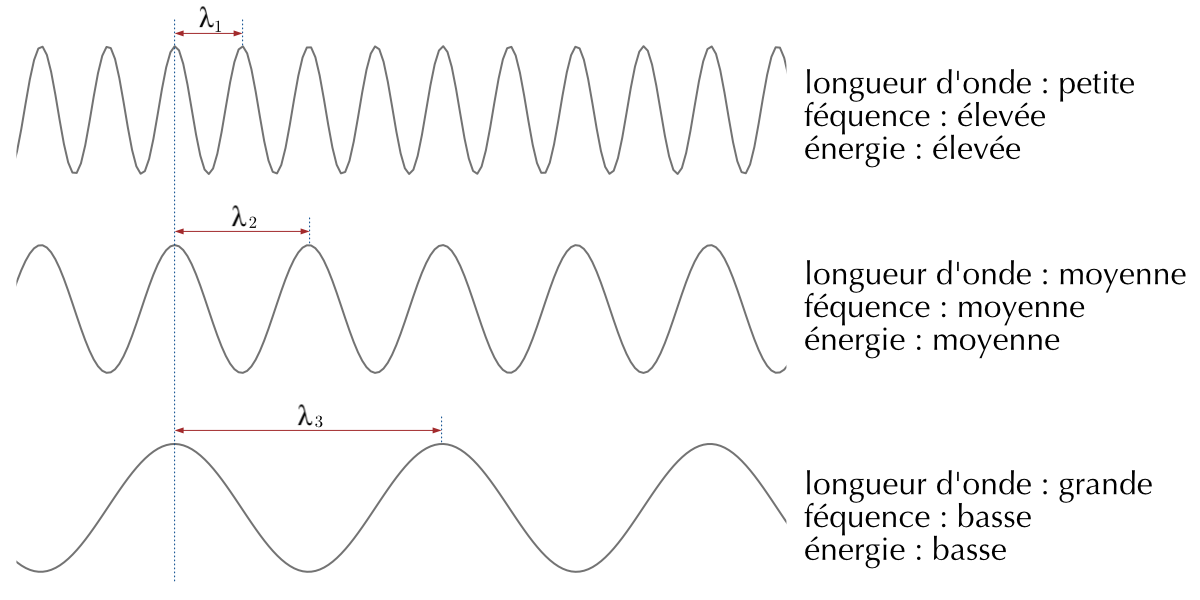
\includegraphics[width=0.75\linewidth]{images/ondes-electromagnetiques} 

}

\caption{Longueur d'onde, fréquence et énergie}\label{fig:ondes-electromagnetiques}
\end{figure}

La longuer d'onde est exprimée en nanomètre, nm, pour les ondes lumineuses. La fréquence est exprimée en Hertz, Hz, le nombre de cycles par seconde. Longueur d'onde et fréquence sont inversément proportionnelles. Plus la longueur d'onde est élevée, plus la fréquence est basse. Plus la longueur d'onde est petite, plus la fréquence est élevée.

\hypertarget{le-spectre-uxe9lectromagnuxe9tique}{%
\subsection{Le spectre électromagnétique}\label{le-spectre-uxe9lectromagnuxe9tique}}

L'analyse du rayonnement émis ou absorbé par la matière s'appelle la \textbf{spectroscopie}.

Le spectre électromagnétique regroupe l'ensemble de toutes les ondes électromagnétiques en fonction de leur longueur d'onde et de leur fréquence.

\begin{figure}

{\centering 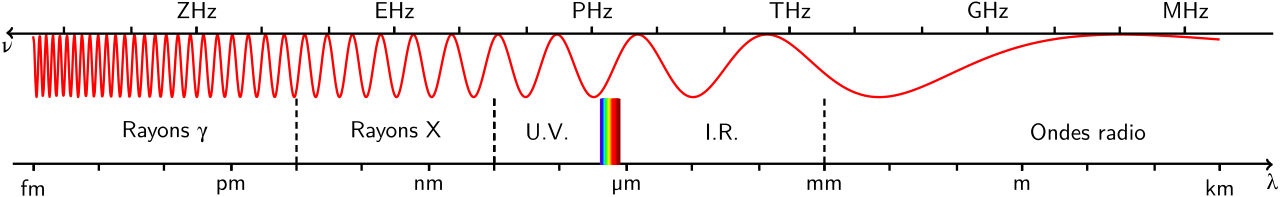
\includegraphics[width=0.95\linewidth]{images/domaine-spectre-electromagnetique} 

}

\caption{Domaines du spectre électromagnétique.}\label{fig:domaine-spectre-electromagnetique}
\end{figure}

\begin{credit}
crédit : wikimedia/Benjamin ABEL

\end{credit}

Les ondes électromagnétiques sont classées en différentes catégories selon leur longueur d'onde. Les plus connues sont celles de la lumière visible (entre 400 et 750 {[}nm{]}, environ) mais il existe d'autres rayonnements que l'oeil ne perçoit pas.

\begin{longtable}[]{@{}lccc@{}}
\caption{\label{tab:domaine-spectre-visible} Domaine du spectre visible.}\tabularnewline
\toprule
couleur & longueur d'onde {[}nm{]} & fréquence {[}10\textsuperscript{14} Hz{]} & énergie {[}eV{]}\tabularnewline
\midrule
\endfirsthead
\toprule
couleur & longueur d'onde {[}nm{]} & fréquence {[}10\textsuperscript{14} Hz{]} & énergie {[}eV{]}\tabularnewline
\midrule
\endhead
violet & 400 & 7.50 & 3.10\tabularnewline
bleu & 450 & 6.66 & 2.75\tabularnewline
cyan & 500 & 5.99 & 2.48\tabularnewline
vert & 550 & 5.45 & 2.25\tabularnewline
jaune & 580 & 5.16 & 2.14\tabularnewline
orange & 600 & 5.00 & 2.06\tabularnewline
rouge & 650 & 4.62 & 1.91\tabularnewline
\bottomrule
\end{longtable}

\hypertarget{interactions-rayonnement-matiuxe8re-1}{%
\subsection{Interactions rayonnement-matière}\label{interactions-rayonnement-matiuxe8re-1}}

Nous sommes régulièrement confrontés à des interactions entre la matière (les atomes) et un rayonnement électromagnétique. Par exemple, un morceau de fer chauffé va émettre un rayonnement électromagnétique différent selon la température à laquelle il est porté. On peut aussi voir l'absorption de rayonnement comme lors d'une radiographie au rayons X. Les os absorbent les rayons X alors que les tissus mous (peau, graisse, muscles) sont quasiment transparents aux rayons X.

Des ondes électromagnétiques peuvent être absorbées par un électron augmentant ainsi son niveau d'énergie au-delà de son \textbf{état fondamental}. Toutefois, un électron n'absorbera une onde que si celle-ci lui permet d'atteindre un niveau d'énergie bien précis. On parlera alors de \textbf{transition électronique} et si l'électron évolue vers un état d'énergie plus élevé, on parlera d'\textbf{excitation électronique}.

Un électron qui se trouve dans un état d'énergie supérieure à celle de l'état fondamental va avoir tendance à évoluer vers un état d'énergie plus faible avec l'émission d'une onde électromagnétique. L'électron va donc perdre de l'énergie en éjectant un photon qui possède exactement la différence d'énergie entre les deux états.

\begin{figure}

{\centering 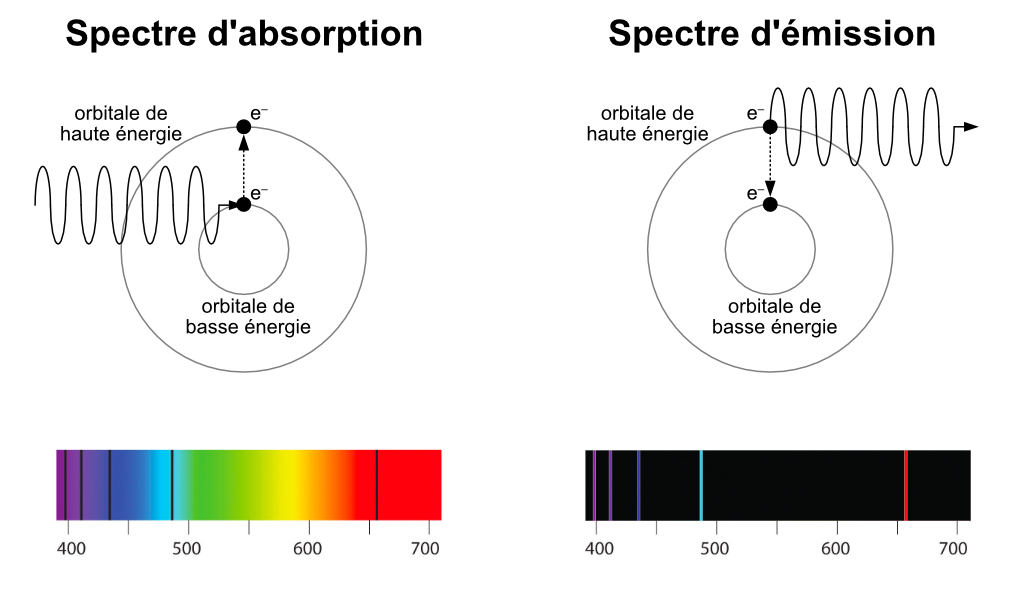
\includegraphics[width=0.5\linewidth]{images/absorption-emission} 

}

\caption{Différence entre spectres d'absorption et d'émission}\label{fig:absorption-emission}
\end{figure}

L'électron absorbe de l'énergie tout en restant au sein de l'atome et finira
toujours par la réémettre sous forme d'une onde électromagnétique. La mesure de ces quantités de lumière émises ou absorbées forment le principe de base de la spectroscopie.

\hypertarget{les-orbitales-atomiques}{%
\section{Les orbitales atomiques}\label{les-orbitales-atomiques}}

Dans les années 1900 Schrödinger développe un modèle atomique plus évolué en utilisant la mécanique quantique, le \textbf{modèle standard}.

Ce modèle introduit une description mathématique du mouvement de l'électron appelée \textbf{orbitale atomique}. Une orbitale représente un volume de l'espace dans lequel la probabilité de trouver un électron est élevée.

\begin{longtable}[]{@{}ccccc@{}}
\caption{\label{tab:couches-sous-couches-orbitales} Résumé des couches, sous-couches et orbitales.}\tabularnewline
\toprule
couche & sous-couche & orbitales & électrons & total électrons\tabularnewline
\midrule
\endfirsthead
\toprule
couche & sous-couche & orbitales & électrons & total électrons\tabularnewline
\midrule
\endhead
\textbf{1} & s & 1 & 2 & \textbf{2}\tabularnewline
\textbf{2} & s & 1 & 2 & \textbf{8}\tabularnewline
& p & 3 & 6 &\tabularnewline
\textbf{3} & s & 1 & 2 & \textbf{18}\tabularnewline
& p & 3 & 6 &\tabularnewline
& d & 5 & 10 &\tabularnewline
\textbf{4} & s & 1 & 2 & \textbf{32}\tabularnewline
& p & 3 & 6 &\tabularnewline
& d & 5 & 10 &\tabularnewline
& f & 7 & 14 &\tabularnewline
\bottomrule
\end{longtable}

Selon ce modèle, les électrons d'un atome gravitent autour de l'atome à des niveaux d'énergie différents. Ces niveaux sont appelés \textbf{couches} et sont situés à différentes distances du noyau. Les couches sont numérotées de 1 à 7 et plus le numéro de la couche est petit, plus la couche est proche du noyau.

Dans une couche les électrons sont distribués en \textbf{sous-couches} d'énergie légèrement différentes. On note les sous-couches avec les lettres s, p, d, f et chacune représente une forme d'orbitale différente.

\begin{figure}

{\centering 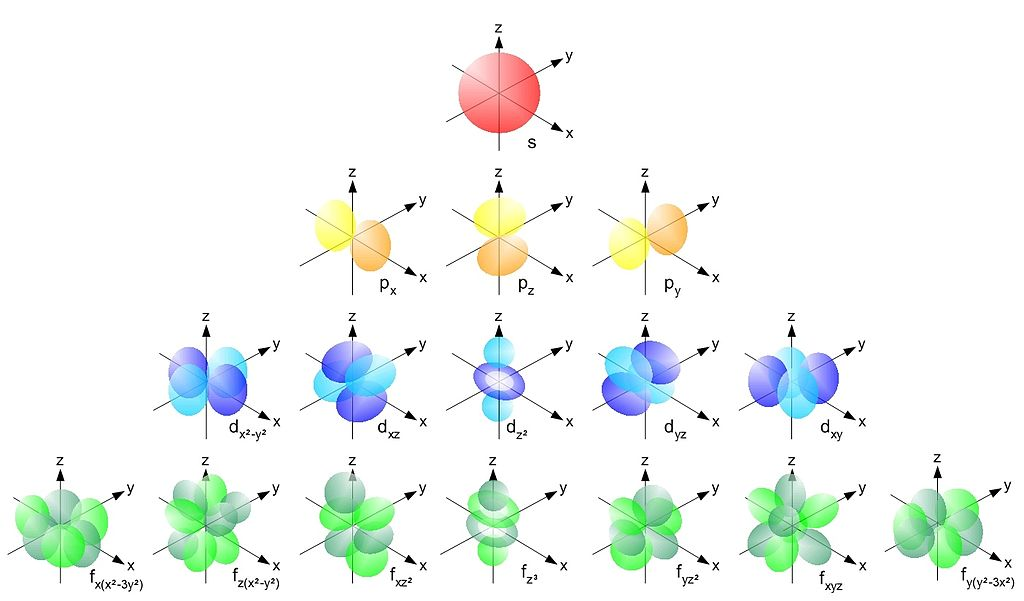
\includegraphics[width=0.9\linewidth]{images/orb-3d} 

}

\caption{Formes des orbitales s, p et d.}\label{fig:orb-3d}
\end{figure}

\begin{credit}
crédit : wikimedia/haade

\end{credit}

Les électrons d'une sous-couche peuvent être répartis dans des volumes d'énergie égale appelés orbitales. Il y a une orbitale pour une sous-couche \emph{s}, trois orbitales pour une \emph{p}, cinq pour une \emph{d}, sept pour un \emph{f}. Une orbitale ne peut être occupée que par deux électrons.

\hypertarget{la-configuration-uxe9lectronique}{%
\subsection{La configuration électronique}\label{la-configuration-uxe9lectronique}}

La manière dont les électrons sont répartis dans les différentes orbitales peut être représenté par un \textbf{diagramme des orbitales atomiques}. Dans ce type de diagramme, les orbitales sont représentées par des cases dans lesquels on place les électrons à disposition. L'orbitale 1s a le niveau d'énergie le plus bas et est la plus proche du noyau.

On utilise ce diagramme pour prédire les liaisons qui se produisent entre deux atomes et pour montrer pourquoi certains éléments se comportent de la même façon.

\begin{figure}

{\centering 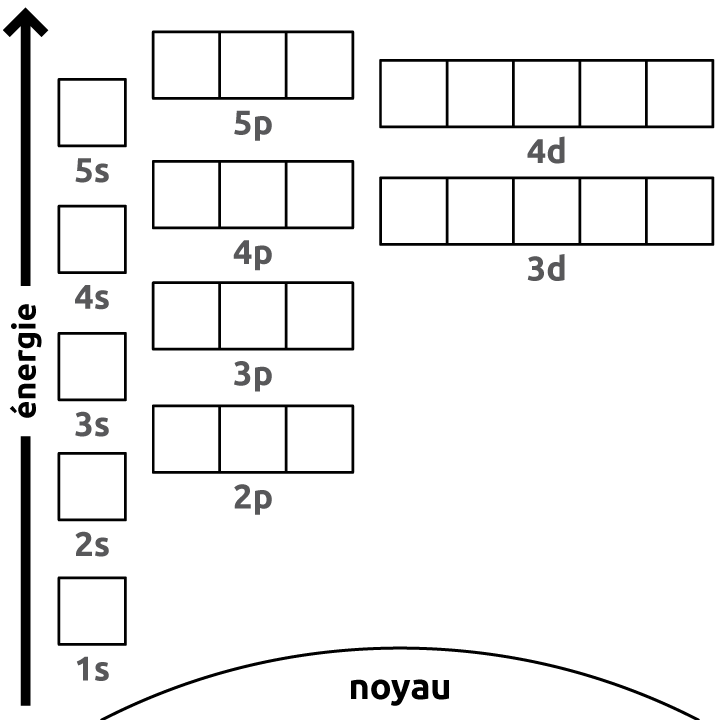
\includegraphics[width=0.4\linewidth]{images/energy-level} 

}

\caption{Diagramme énergétique des orbitales atomiques.}\label{fig:energy-level}
\end{figure}

\newpage

\hypertarget{duxe9terminer-une-configuration-uxe9lectronique}{%
\subsection{Déterminer une configuration électronique}\label{duxe9terminer-une-configuration-uxe9lectronique}}

\begin{figure}

{\centering 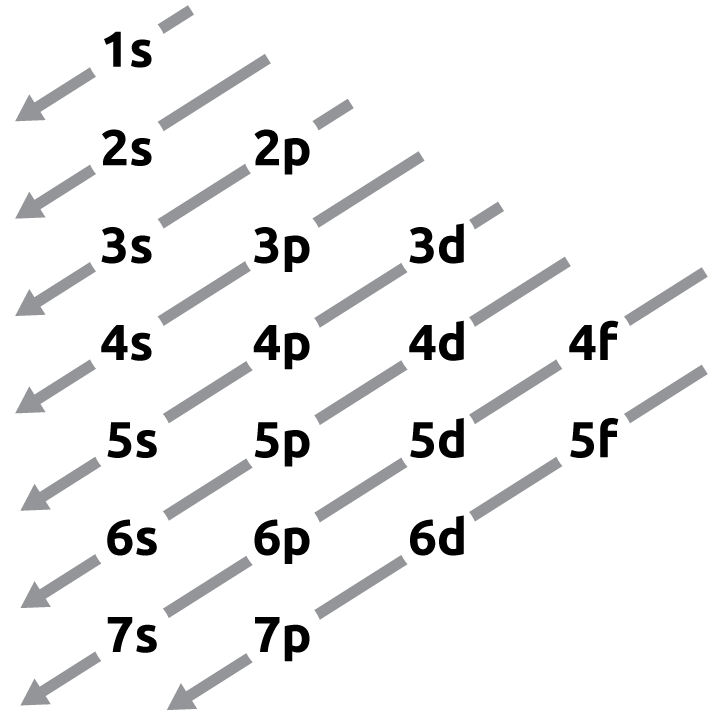
\includegraphics[width=0.25\linewidth]{images/energy-level-order} 

}

\caption{Ordre de remplissage des orbitales.}\label{fig:energy-level-order}
\end{figure}

En connaissant le nombre d'électrons contenus dans un atome, on peut remplir ce diagramme en respectant certaines règles:

\begin{itemize}
\tightlist
\item
  Les électrons sont placés dans la sous-couche disponible de plus basse énergie.
\item
  On peut placer au maximum 2 électrons dans une orbitale (exclusion de Pauli).
\item
  La figure \ref{fig:energy-level-order} donne l'ordre de remplissage des orbitales (principe Aufbau).
\item
  Si plusieurs orbitales de même énergie sont disponibles, on remplit le plus d'orbitales possibles avant d'apparier les électrons.
\end{itemize}

Une fois le diagramme rempli, on en déduit la configuration électronique de l'atome pour le niveau de plus basse énergie. La \textbf{configuration électronique} d'un atome est une notation abrégée de la répartition des électrons dans les différentes couches et sous-couches électroniques.

\begin{Exercise}
A l'aide des diagrammes suivants, déterminez la configuration électronique de l'atome de carbone et celle de l'atome de sodium :

\end{Exercise}

\begin{longtable}[]{@{}ll@{}}
\toprule
atome de carbone & atome de sodium\tabularnewline
\midrule
\endhead
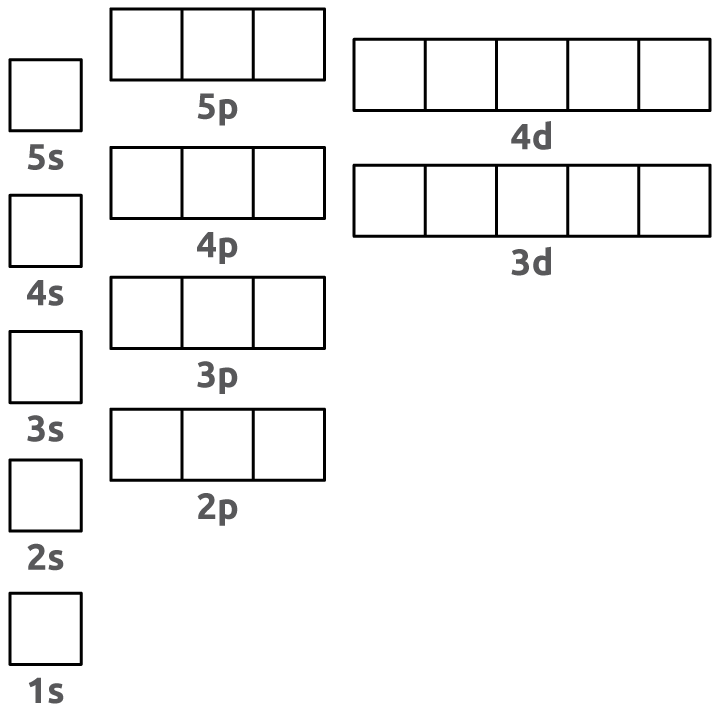
\includegraphics[width=0.4\textwidth,height=\textheight]{images/energy-level-2.png} & 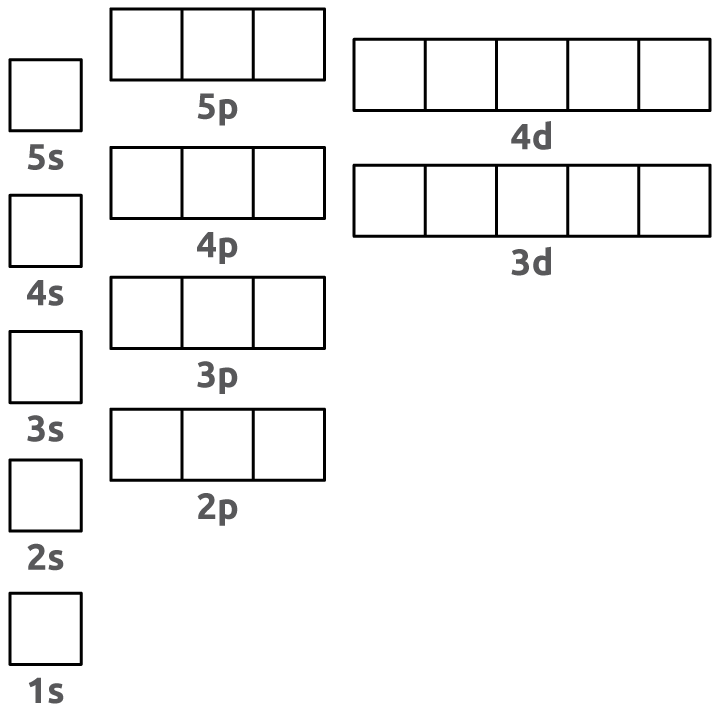
\includegraphics[width=0.4\textwidth,height=\textheight]{images/energy-level-2.png}\tabularnewline
nombre d'électrons : & nombre d'électrons :\tabularnewline
structure électronique : & structure électronique :\tabularnewline
\bottomrule
\end{longtable}

\begin{Answer}

\begin{itemize}
\tightlist
\item
  atome de carbone\\
  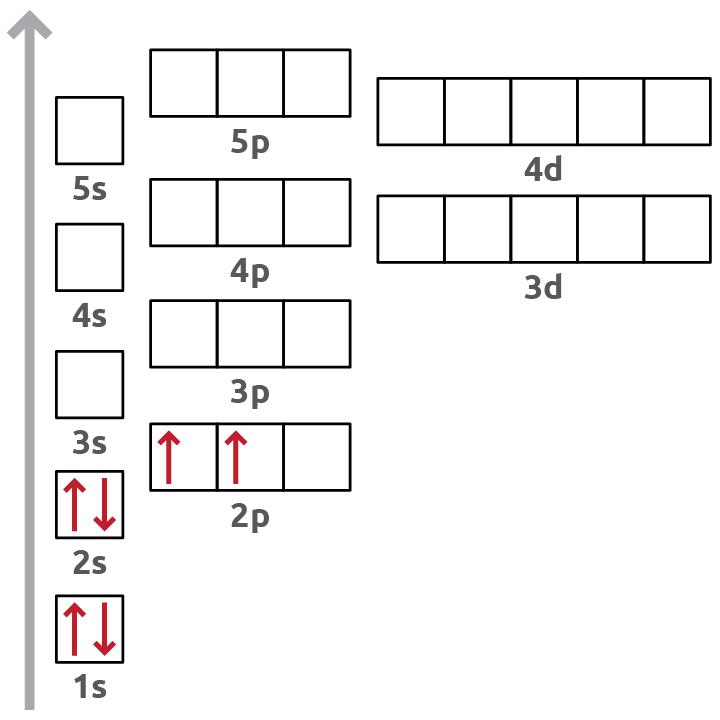
\includegraphics[width=0.33\textwidth,height=\textheight]{images/energy-level-2-2.png}

  \begin{itemize}
  \tightlist
  \item
    nombre d'électrons : \textbf{6}
  \item
    structure électronique : \(1s^2 2s^2 2p^2\)
  \end{itemize}
\item
  atome de sodium\\
  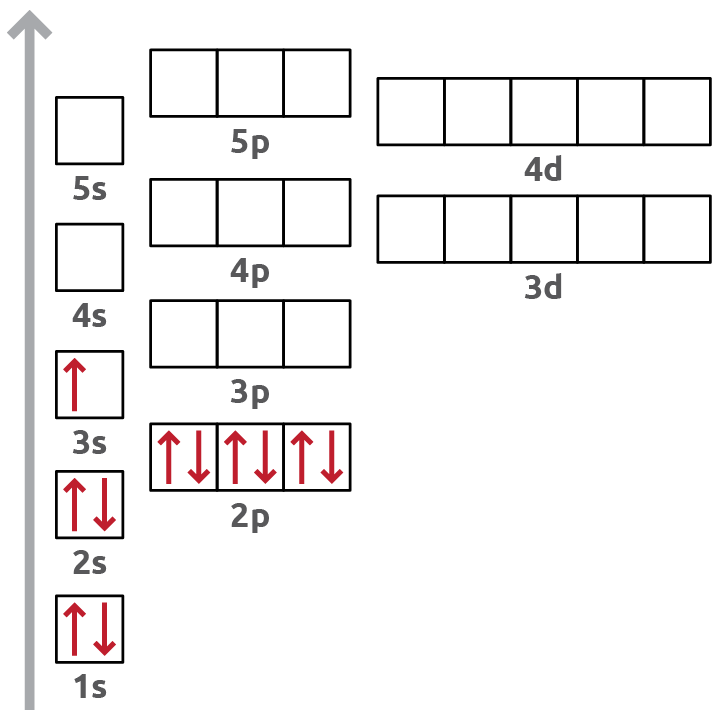
\includegraphics[width=0.33\textwidth,height=\textheight]{images/energy-level-2-3.png}

  \begin{itemize}
  \tightlist
  \item
    nombre d'électrons : \textbf{11}
  \item
    structure électronique : \(1s^2 2s^2 2p^6 3s^1\)
  \end{itemize}
\end{itemize}


\end{Answer}

Pour simplifier la notation de la configuration électronique, on indique que les électrons de la dernière couche électronique. On remplace les autres couches par le symbole du gaz rare le plus proche entre crochets. Par exemple, la structure électronique du chlore (Cl) :

\[ \underbrace{1s^{2}~2s^{2}~2p^{6}}_{\text{Néon}}~3s^{2}~3p^{5} \text{ devient } [Ne]~3s^{2}~3p^{5} \]

\begin{longtable}[]{@{}cclcl@{}}
\caption{\label{tab:conf-elec-premieres-periodes} Configuration électronique des deux premières périodes.}\tabularnewline
\toprule
Groupe & Elément & Conf. électronique & Elément & Conf. électronique\tabularnewline
\midrule
\endfirsthead
\toprule
Groupe & Elément & Conf. électronique & Elément & Conf. électronique\tabularnewline
\midrule
\endhead
IA & Li & {[}He{]} \(2s^{1}\) & Na & {[}Ne{]} \(3s^{1}\)\tabularnewline
IIA & Be & {[}He{]} \(2s^{2}\) & Mg & {[}Ne{]} \(3s^{2}\)\tabularnewline
IIIA & B & {[}He{]} \(2s^{2}~2p^{1}\) & Al & {[}Ne{]} \(3s^{2}~3p^{1}\)\tabularnewline
IVA & C & {[}He{]} \(2s^{2}~2p^{2}\) & Si & {[}Ne{]} \(3s^{2}~3p^{2}\)\tabularnewline
VA & N & {[}He{]} \(2s^{2}~2p^{3}\) & P & {[}Ne{]} \(3s^{2}~3p^{3}\)\tabularnewline
VIA & O & {[}He{]} \(2s^{2}~2p^{4}\) & S & {[}Ne{]} \(3s^{2}~3p^{4}\)\tabularnewline
VIIA & F & {[}He{]} \(2s^{2}~2p^{5}\) & Cl & {[}Ne{]} \(3s^{2}~3p^{5}\)\tabularnewline
VIIIA & Ne & {[}He{]} \(2s^{2}~2p^{6} \equiv\) {[}Ne{]} & Ar & {[}He{]} \$3s\textsuperscript{\{2\}\textasciitilde3p}\{6\} \equiv \$ {[}Ar{]}\tabularnewline
\bottomrule
\end{longtable}

La configuration électronique du niveau de plus basse énergie est appelée \textbf{état fondamental}. Les configurations dont la distribution des électrons est différente de l'état fondamental sont appelées \textbf{états excités}.

\begin{figure}

{\centering 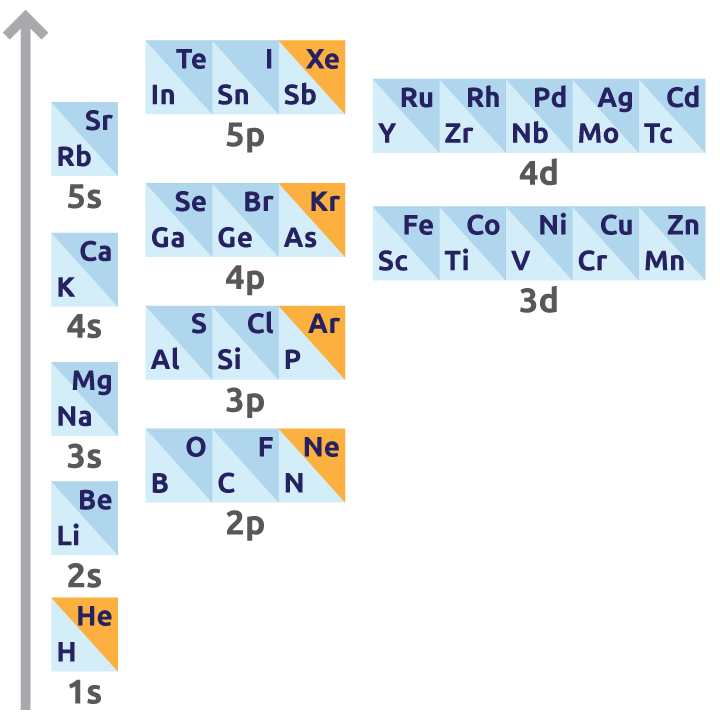
\includegraphics[width=0.45\linewidth]{images/energy-level-5} 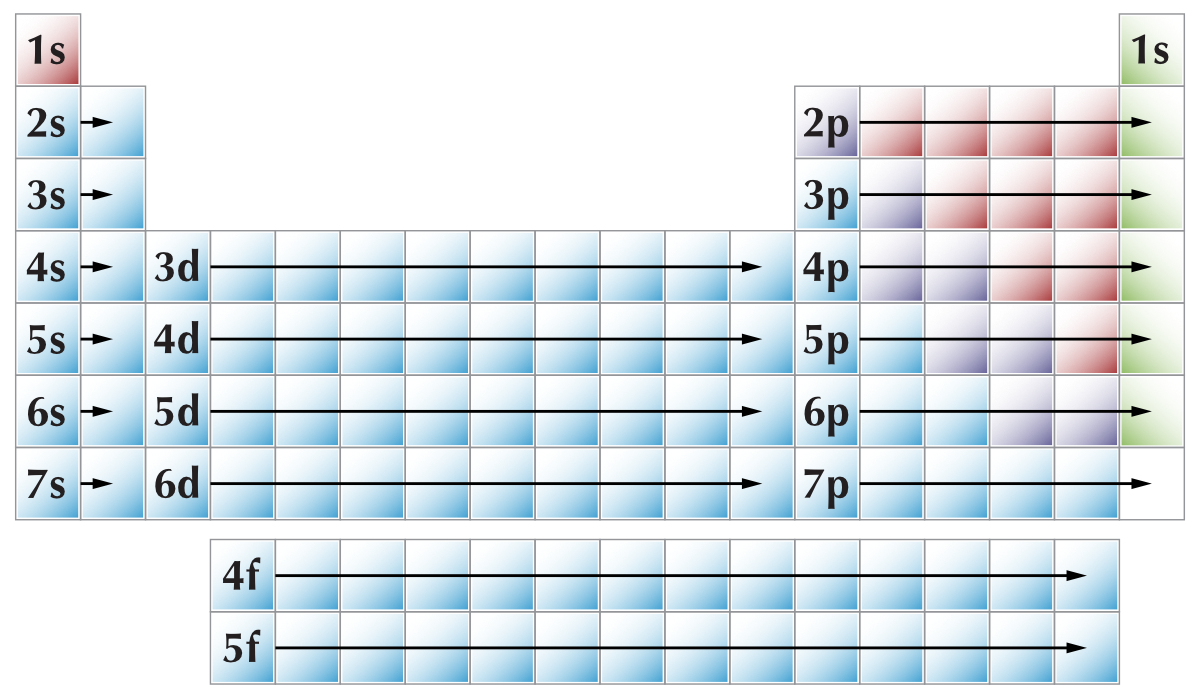
\includegraphics[width=0.45\linewidth]{images/tpe-orbitals} 

}

\caption{Les orbitales atomiques et le tableau périodique.}\label{fig:energy-level-5}
\end{figure}

\hypertarget{les-uxe9lectrons-de-valence}{%
\section{Les électrons de valence}\label{les-uxe9lectrons-de-valence}}

\begin{tcolorbox}
\textbf{Les électrons de valence}\\
Les électrons de valence sont les électrons de la dernière couche électronique d'un atome.

\end{tcolorbox}

Lorsqu'un chimiste étudie une réaction, il étudie les électrons transféré entre les acteurs de la réaction. Les électrons dont le niveau d'énergie est le plus éloigné du noyau seront retenus de manière moins forte. Ce sont donc ces électrons qui seront impliqués dans les réactions.

\begin{figure}

{\centering 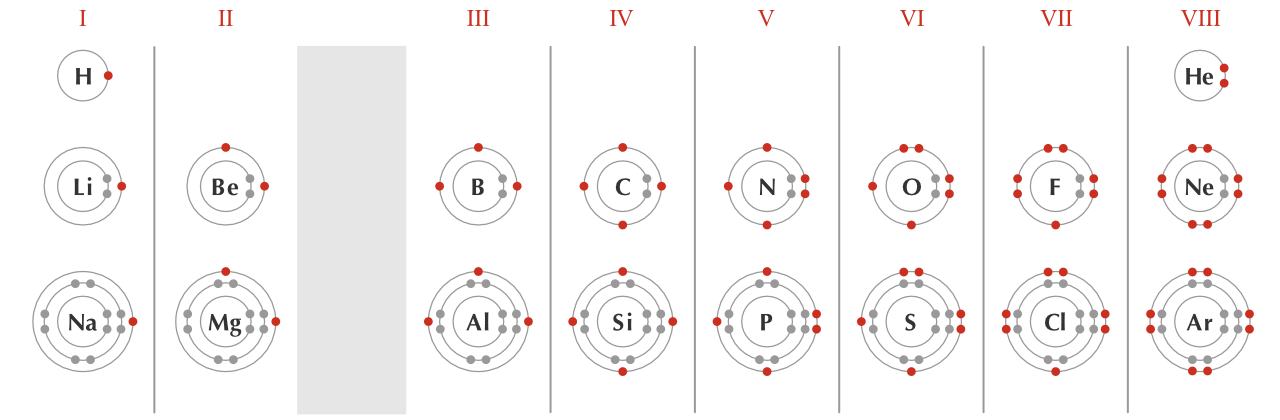
\includegraphics[width=1\linewidth]{images/configuration-electronique} 

}

\caption{Répartition électronique des trois premières périodes.}\label{fig:configuration-electronique}
\end{figure}

Le chimiste américain \textbf{G. N. Lewis} (1875-1946) a proposé un moyen simple de représenter les électrons de valence d'un atome. C'est ce qu'on appelle la \textbf{structure de Lewis}.

On utilise les règles suivantes pour dessiner la structure de Lewis d'un atome:

\begin{itemize}
\tightlist
\item
  Le nombre d'électrons valence est égal au numéro du groupe (IA à VIIIA).
\item
  On place un point à la fois sur chacun des quatre côtés du symbole d'élément.
\item
  On continue d'ajouter des points, en les appariant, jusqu'à ce que tous les électrons de valence soient utilisés.
\end{itemize}

\begin{longtable}[]{@{}cccccccc@{}}
\caption{\label{tab:structure-lewis-groupe-principal} Structure de Lewis des éléments du groupe principal (c = célibataire, p = paire).}\tabularnewline
\toprule
I & II & II & IV & V & VI & VII & VII\tabularnewline
\midrule
\endfirsthead
\toprule
I & II & II & IV & V & VI & VII & VII\tabularnewline
\midrule
\endhead
\includegraphics[width=3em,height=\textheight]{images/lewis-dots-1c.png} & \includegraphics[width=3em,height=\textheight]{images/lewis-dots-2c.png} & \includegraphics[width=3em,height=\textheight]{images/lewis-dots-3c.png} & \includegraphics[width=3em,height=\textheight]{images/lewis-dots-4c.png} & \includegraphics[width=3em,height=\textheight]{images/lewis-dots-1p3c.png} & \includegraphics[width=3em,height=\textheight]{images/lewis-dots-2p2c.png} & \includegraphics[width=3em,height=\textheight]{images/lewis-dots-3p1c.png} & \includegraphics[width=3em,height=\textheight]{images/lewis-dots-4p.png}\tabularnewline
1c & 2c & 3c & 4c & 1p 3c & 2p 2c & 3p 1c & 4p\tabularnewline
\bottomrule
\end{longtable}

\newpage

\begin{Exercise}
Dessinez la structure de Lewis des éléments des trois premières périodes.

\end{Exercise}

\begin{longtable}[]{@{}cccccccc@{}}
\toprule
I & II & II & IV & V & VI & VII & VII\tabularnewline
\midrule
\endhead
Hydrogène & & & & & & & Hélium\tabularnewline
\includegraphics[width=\textwidth,height=4em]{images/1px.png} & \includegraphics[width=\textwidth,height=4em]{images/1px.png} & \includegraphics[width=\textwidth,height=4em]{images/1px.png} & \includegraphics[width=\textwidth,height=4em]{images/1px.png} & \includegraphics[width=\textwidth,height=4em]{images/1px.png} & \includegraphics[width=\textwidth,height=4em]{images/1px.png} & \includegraphics[width=\textwidth,height=4em]{images/1px.png} & \includegraphics[width=\textwidth,height=4em]{images/1px.png}\tabularnewline
Lithium & Béryllium & Bore & Carbone & Azote & Oxygène & Fluor & Néon\tabularnewline
\includegraphics[width=\textwidth,height=4em]{images/1px.png} & \includegraphics[width=\textwidth,height=4em]{images/1px.png} & \includegraphics[width=\textwidth,height=4em]{images/1px.png} & \includegraphics[width=\textwidth,height=4em]{images/1px.png} & \includegraphics[width=\textwidth,height=4em]{images/1px.png} & \includegraphics[width=\textwidth,height=4em]{images/1px.png} & \includegraphics[width=\textwidth,height=4em]{images/1px.png} & \includegraphics[width=\textwidth,height=4em]{images/1px.png}\tabularnewline
Sodium & Magnésium & Aluminium & Silicium & Phosphore & Soufre & Chlore & Argon\tabularnewline
\includegraphics[width=\textwidth,height=4em]{images/1px.png} & \includegraphics[width=\textwidth,height=4em]{images/1px.png} & \includegraphics[width=\textwidth,height=4em]{images/1px.png} & \includegraphics[width=\textwidth,height=4em]{images/1px.png} & \includegraphics[width=\textwidth,height=4em]{images/1px.png} & \includegraphics[width=\textwidth,height=4em]{images/1px.png} & \includegraphics[width=\textwidth,height=4em]{images/1px.png} & \includegraphics[width=\textwidth,height=4em]{images/1px.png}\tabularnewline
\bottomrule
\end{longtable}

\hypertarget{la-ruxe8gle-de-loctet}{%
\section{La règle de l'octet}\label{la-ruxe8gle-de-loctet}}

Les gaz rares (groupe VIIIA) sont très peu réactifs car ils ont une très grande stabilité électronique. Ceci est dû au fait que leur couche électronique de valence est complètement remplie avec \textbf{huit électrons}, à l'exception de l'hélium, qui en a deux.

Cette observation a conduit à une règle connue sous le nom de \textbf{règle de l'octet}.

\begin{tcolorbox}
\textbf{Règle de l'octet}\\
Les atomes ont tendance à gagner, perdre, ou partager des électrons pour avoir huit électrons dans leur couche de valence.

\end{tcolorbox}

Le remplissage complet de la couche électronique de valence est le moteur des réactions chimiques.

\hypertarget{les-ions}{%
\section{Les ions}\label{les-ions}}

\begin{tcolorbox}
\textbf{Ion}\\
Un ion est un atome ou un groupe d'atomes qui a gagné ou perdu un ou plusieurs électrons.

\end{tcolorbox}

Les atomes qui \textbf{perdent} un ou plusieurs électrons ont un excédent de charge positive et sont appelés \textbf{cations}.

\hypertarget{le-cation-ou-la-perte-duxe9lectrons}{%
\subsection{Le cation ou la perte d'électrons}\label{le-cation-ou-la-perte-duxe9lectrons}}

Prenons, par exemple, le sodium. Son numéro atomique est égal à 11, il contient 11 protons et comme l'atome est neutre, il contient également 11 électrons. Avec un électron en moins, l'atome est constitué de 11 protons et 10 électrons. Il a donc une charge positive en excès. il devient un cation. On écrira le cation sodium \textbf{Na\textsuperscript{+}}.

\[ \begin{split}
        Na \rightarrow Na^+ + 1e^-
    \end{split}
    \qquad
    \begin{split}
        11\:p^{+}\:+\:10\:e^{-}\:=\:\text{1 charge positive}\:=\:+1
    \end{split} \]

Les atomes qui ont des configurations électroniques équivalentes sont appelés \textbf{isoélectroniques}. Le cation sodium est isoélectronique avec le néon.

\hypertarget{lanion-ou-le-gain-duxe9lectrons}{%
\subsection{L'anion ou le gain d'électrons}\label{lanion-ou-le-gain-duxe9lectrons}}

Les atomes qui \textbf{gagnent} un ou plusieurs électrons ont un excédent de charge négative et sont appelés \textbf{anions}.

Prenons, par exemple, le chlore. Son numéro atomique est égal à 17, il contient 17 protons et 17 électrons. Avec un électron en plus, l'atome est constitué de 17 protons et 18 électrons. Il a donc une charge négative en excès. il devient un anion. On écrira l'anion chlore \textbf{Cl\textsuperscript{-}}.

\[ \begin{split}
        Cl + 1e^- \rightarrow Cl^-
    \end{split}
    \qquad
    \begin{split}
        17\:p^{+}\:+\:18\:e^{-}\:=\:\text{1 charge négative}\:=\: -1
    \end{split} \]

L'anion chlore est isoélectronique avec l'argon.

\begin{Exercise}

Déterminer quelle sera la charge des atomes correspondant aux description suivante:

\begin{enumerate}
\def\labelenumi{\arabic{enumi}.}
\tightlist
\item
  Un atome ayant perdu deux électrons\\
\item
  Un atome ayant gagné un électron\\
\item
  Un atome ayant perdu trois électrons\\
\item
  Un atome ayant gagné deux électrons\\
\item
  Un atome ayant perdu un électron\\
\item
  Un atome ayant gagné trois électrons
\end{enumerate}


\end{Exercise}

\begin{Answer}

\begin{enumerate}
\def\labelenumi{\arabic{enumi}.}
\tightlist
\item
  0 - (2e-) = +2
\item
  0 + (1e-) = -1
\item
  0 - (3e-) = +3
\item
  0 + (2e-) = -2
\item
  0 - (1e-) = +1
\item
  0 + (3e-) = -3
\end{enumerate}

\newpage


\end{Answer}

\hypertarget{les-ions-stables---groupe-a}{%
\subsection{Les ions stables - groupe A}\label{les-ions-stables---groupe-a}}

Le gain ou la perte de un, deux, ou parfois même trois électrons est possible, mais en général, un atome ne perd ou ne gagne pas plus de trois électrons.

La règle de l'octet nous indique qu'un atome avec huit électrons dans sa couche électronique de valence devient énergétiquement stable. Les \textbf{ions stables} formés par les atomes sont donc ceux qui confirment la règle de l'octet.

Dans le tableau périodique, les chiffres romains des groupes A indiquent le nombre d'électrons de valence de chaque élément. On peut utiliser la position d'un élément dans le tableau pour déterminer quel sera l'ion stable formé par cet élément.

\begin{Exercise}
Représenter sous leur forme symbolique les ions stables formés par les éléments des périodes n°2 et n°3.

\end{Exercise}

\begin{longtable}[]{@{}cccccccc@{}}
\toprule
I & II & II & IV & V & VI & VII & VII\tabularnewline
\midrule
\endhead
Lithium & Béryllium & Bore & Carbone & Azote & Oxygène & Fluor & Néon\tabularnewline
\includegraphics[width=\textwidth,height=4em]{images/1px.png} & \includegraphics[width=\textwidth,height=4em]{images/1px.png} & \includegraphics[width=\textwidth,height=4em]{images/1px.png} & \includegraphics[width=\textwidth,height=4em]{images/1px.png} & \includegraphics[width=\textwidth,height=4em]{images/1px.png} & \includegraphics[width=\textwidth,height=4em]{images/1px.png} & \includegraphics[width=\textwidth,height=4em]{images/1px.png} & \includegraphics[width=\textwidth,height=4em]{images/1px.png}\tabularnewline
Sodium & Magnésium & Aluminium & Silicium & Phosphore & Soufre & Chlore & Argon\tabularnewline
\includegraphics[width=\textwidth,height=4em]{images/1px.png} & \includegraphics[width=\textwidth,height=4em]{images/1px.png} & \includegraphics[width=\textwidth,height=4em]{images/1px.png} & \includegraphics[width=\textwidth,height=4em]{images/1px.png} & \includegraphics[width=\textwidth,height=4em]{images/1px.png} & \includegraphics[width=\textwidth,height=4em]{images/1px.png} & \includegraphics[width=\textwidth,height=4em]{images/1px.png} & \includegraphics[width=\textwidth,height=4em]{images/1px.png}\tabularnewline
\bottomrule
\end{longtable}

\hypertarget{les-ions-des-uxe9luxe9ments-de-transition---groupe-b}{%
\subsection{Les ions des éléments de transition - groupe B}\label{les-ions-des-uxe9luxe9ments-de-transition---groupe-b}}

Déterminer l'ion stable formé par les métaux de transition est plus difficile car ces éléments ne gagneront ou ne perderont pas toujours le même nombre d'électrons.

Les éléments de transition ne respectent pas la règle de l'octet, mais une autre règle appelée la \textbf{règle des 18 électrons}. Nous n'aborderons pas cette règle dans le cadre de ce cours.

\newpage

\hypertarget{exercices-suppluxe9mentaires-4}{%
\section{Exercices supplémentaires}\label{exercices-suppluxe9mentaires-4}}

\begin{Exercise}

Représenter sous leur forme symbolique les ions stables formés par les éléments des périodes n°2 et n°3.

\begin{enumerate}
\def\labelenumi{\arabic{enumi}.}
\tightlist
\item
  Donnez le symbole des éléments suivants :
  Magnésium, Potassium, Fer, Cuivre\\
  \vspace{\stretch{1}}
\item
  Quel est le nom des éléments suivants :
  C, Cl, Au, Sb\\
  \vspace{\stretch{1}}
\item
  Dans quelle période se trouvent les éléments suivants :
  He, Ge, Rb, I\\
  \vspace{\stretch{1}}
\item
  Dans quel groupe se trouvent les éléments suivants :
  Soufre, Iode, Ca, Sn\\
  \vspace{\stretch{1}}
\item
  Proposez le symbole d'un élément correspondant à chacune des descriptions suivantes :
\end{enumerate}

\begin{itemize}
\tightlist
\item
  un halogène
\item
  un non-métal
\item
  un métal alcalin
\item
  un élément de transition
\item
  un gaz rare
\item
  un métal alcalino-terreux
\end{itemize}


\end{Exercise}

\begin{Answer}

\begin{enumerate}
\def\labelenumi{\arabic{enumi}.}
\tightlist
\item
  Donnez le symbole des éléments suivants :\\
  Magnésium : Mg / Potassium : K / Fer : Fe / Cuivre : Cu
\item
  Quel est le nom des éléments suivants :\\
  C : Carbone- Cl : Chlore / Au : Or / Sb : Antimoine
\item
  Dans quelle période se trouvent les éléments suivants :\\
  He : 1 / Ge : 4 / Rb : 5 / I : 5
\item
  Dans quel groupe se trouvent les éléments suivants :\\
  Soufre : VI / Iode : VII / Ca : II / Sn : IV
\end{enumerate}


\end{Answer}

\begin{Exercise}

Pour chaque descritpion ci-dessous, déterminez la charge de l'atome, indiquez si l'élément est un cation ou un anion et donnez son symbole.

\begin{enumerate}
\def\labelenumi{\arabic{enumi}.}
\tightlist
\item
  un atome de magnésium avec 12 protons et 10 électrons\\
\item
  un atome de fluor avec 9 protons et 10 électrons\\
\item
  un atome de lithium avec 3 protons et 2 électrons\\
\item
  un atome de soufre avec 16 protons et 18 électrons
\end{enumerate}


\end{Exercise}

\begin{Answer}

\begin{enumerate}
\def\labelenumi{\arabic{enumi}.}
\tightlist
\item
  +2, cation, \(Mg^{+2}\)
\item
  -1, anion, \(F^-\)
\item
  +1, cation \(Li^+\)
\item
  -2, anion, \(S^{-2}\)
\end{enumerate}


\end{Answer}

\newpage

\begin{Exercise}

Donnez le nom et le symbole des éléments qui correspondent aux descriptions suivantes.

\begin{enumerate}
\def\labelenumi{\arabic{enumi}.}
\tightlist
\item
  27 protons dans le noyau de chaque atome\\
\item
  50 électrons dans chaque atome neutre\\
\item
  18 électrons dans chaque cation +2\\
\item
  10 électrons dans chaque anion -1
\end{enumerate}


\end{Exercise}

\begin{Answer}

\begin{enumerate}
\def\labelenumi{\arabic{enumi}.}
\tightlist
\item
  Cobalt / Co
\item
  Étain / Sn
\item
  Calcium / Ca
\item
  Fluor / F
\end{enumerate}


\end{Answer}

\begin{Exercise}

Indiquer le nombre de protons, de neutrons et d'électrons de chacune des espèces suivantes.

\begin{enumerate}
\def\labelenumi{\arabic{enumi}.}
\tightlist
\item
  \(^{90}Sr\)\\
\item
  \(^{41}K\)\\
\item
  \(^{75}_{33}As\)\\
\item
  \(^{32}_{15}P\)\\
\item
  \(^{90}As^{+2}\)\\
\item
  \(^{34}_{16}S^{-2}\)
\end{enumerate}


\end{Exercise}

\begin{Answer}

\begin{enumerate}
\def\labelenumi{\arabic{enumi}.}
\tightlist
\item
  \(^{90}Sr\) : 38 \(p^+\) / 52 \(n\) / 38 \(e^-\)
\item
  \(^{41}K\) : 19 \(p^+\) / 22 \(n\) / 19 \(e^-\)
\item
  \(^{75}_{33}As\) : 33 \(p^+\) / 42 \(n\) / 33 \(e^-\)
\item
  \(^{32}_{15}P\) : 15 \(p^+\) / 17 \(n\) / 15 \(e^-\)
\item
  \(^{90}As^{+2}\) : 33 \(p^+\) / 57 \(n\) / 31 \(e^-\)
\item
  \(^{34}_{16}S^{-2}\) : 16 \(p^+\) / 18 \(n\) / 18 \(e^-\)
\end{enumerate}


\end{Answer}

\begin{Exercise}

Dessinez le symbole de Lewis de chacun des éléments suivants : Al, Br, Ar, Ca.

\vspace{\stretch{1}}


\end{Exercise}

\begin{Exercise}

A l'aide du tableau périodique, indiquez quel sera l'ion stable formé par les éléments suivants : Na, Mg, Cl, K, Al, S, Ca, Ga.

\vspace{\stretch{1}}


\end{Exercise}

\begin{Answer}

\begin{itemize}
\tightlist
\item
  Na : \(Na^+\)
\item
  Mg : \(Mg^{2+}\)
\item
  Cl : \(Cl^-\)
\item
  K : \(K^+\)
\item
  Al : \(Al^{3+}\)
\item
  S : \(S^{2-}\)
\item
  Ca : \(Ca^{2+}\)
\item
  Ga : \(Ga^{3+}\)
\end{itemize}


\end{Answer}

\newpage

\section{Solutions des exercices} \shipoutAnswer

\hypertarget{moluxe9cules-et-liaisons-chimiques}{%
\chapter{Molécules et liaisons chimiques}\label{moluxe9cules-et-liaisons-chimiques}}

\begin{objectives}

\begin{itemize}
\tightlist
\item
  Expliquer le concept de liaison chimique.
\item
  Identifier les différents types de liaisons chimiques.
\item
  Expliquer le concept d'électronégativité.
\item
  Reconnaître les ions que contient une molécule dans sa formule brute.
\item
  Dessiner la formule développée d'une molécule avec ses covalences et électrovalences.
\item
  Calculer la masse réelle d'une molécule à partir des masses atomiques des atomes qui la composent.
\item
  Calculer le nombre de moles/molécules que contient une masse donnée d'un composé.
\end{itemize}


\end{objectives}

En observant le monde autour de nous, on découvre qu'il est composé principalement de corps purs composés et de mélanges de corps purs composés: la roche, les sols, le pétrole, les arbres et le corps humain sont tous des mélanges complexes de composés chimiques liant différents types d'atomes ensemble. \textbf{Seuls les gaz rares se trouvent dans la nature sous forme d'atomes isolés.}

\hypertarget{les-moluxe9cules}{%
\section{Les molécules}\label{les-moluxe9cules}}

De nombreuses substances existent sous la forme de deux ou plusieurs atomes reliés entre eux de manière si forte qu'ils se comportent comme une seule particule. Ces combinaisons de plusieurs atomes sont appelées molécules. De manière similaire à un atome, une molécule est la plus petite partie d'une substance qui possède les propriétés physiques et chimiques de cette substance. Cependant, une molécule est composée de plus d'un atome.

\begin{tcolorbox}
\textbf{Molécule}\\
Une molécule est un groupe d'au moins deux atomes liés par une/des liaison(s) chimique(s).

\end{tcolorbox}

Les chimistes utilisent des formules chimiques pour exprimer la composition des espèces chimiques à l'aide de symboles.

\hypertarget{la-formule-brute}{%
\subsection{La formule brute}\label{la-formule-brute}}

Les molécules sont composées d'atomes. On les représente par une formule, en indiquant les symboles des atomes qui les composent et leur nombre. Cette formule est appelée \textbf{formule brute}. La formule brute donne le nombre d'atomes des différents éléments qui forment un composé, exprimés avec les plus petits nombres entiers possibles.

\begin{itemize}
\tightlist
\item
  \(NaCl\) : 1 atome de sodium et 1 atome de chlore\\
\item
  \(O_2\) : 2 atomes d'oxygène\\
\item
  \(H_2O\) : 2 atomes d'hydrogène et 1 atome d'oxygène
\end{itemize}

Lorsqu'un atome n'est présent qu'une seule fois dans la molécule, on n'indique pas l'indice 1. La formule brute de l'eau s'écrira donc H\textsubscript{2}O et non H\textsubscript{2}O\textsubscript{1}, et on écrira CO\textsubscript{2} et non C\textsubscript{1}O\textsubscript{2}.

\hypertarget{la-masse-molaire-moluxe9culaire}{%
\section{La masse molaire moléculaire}\label{la-masse-molaire-moluxe9culaire}}

\begin{tcolorbox}
\textbf{Masse molaire moléculaire}\\
La masse molaire d'un composé est la masse en grammes d'une mole de molécules de ce composé.

\end{tcolorbox}

Une molécule de \(CH_4\) contient 1 atome de carbone et 4 atomes d'hydrogène.

Donc, une mole de molécules de \(CH_4\) contient 1 mole d'atomes de carbone et 4 moles d'atomes d'hydrogène.

La masse d'une mole de méthane peut être trouvée en additionnant les masses molaires atomiques du carbone et de l'hydrogène présents dans la molécule:

\[ \begin{split}
  \text{Masse de 1 [mol] de carbone} &= 12.01 [g] \\
  \text{Masse de 4 [mol] d'hydrogène} &= 4.032 [g] \quad (4 \cdot 1.008 [g]) \\
  \hline
  \text{Masse de 1 [mol] de $CH_4$} &= 16.04 [g]
  \end{split} \]

\hypertarget{la-formule-duxe9veloppuxe9e}{%
\subsection{La formule développée}\label{la-formule-duxe9veloppuxe9e}}

La formule brute ne permet pas d'indiquer comment les atomes sont reliés entre eux par des liaisons chimiques ou comment ils sont disposés dans l'espace. Comprendre comment les atomes d'une molécule sont disposés et comment ils sont liés entre eux permet d'expliquer les caractéristiques physiques et chimique d'un composé.

\textbf{La formule développée} identifie l'emplacement des atomes ainsi que leurs liaisons au sein d'une molécule. On utilise la représentation de Lewis pour dessiner les atomes des différents éléments qui sont reliés par des lignes qui représentent les liaisons chimiques.

\begin{figure}

{\centering \includegraphics[width=1\linewidth]{images/methanol-formulas} 

}

\caption{La molécule de méthanol.}\label{fig:methanol-formulas}
\end{figure}

\hypertarget{les-liaisons-chimiques}{%
\section{Les liaisons chimiques}\label{les-liaisons-chimiques}}

Pourquoi les atomes se lient entre eux ? Deux atomes liés ensemble forment un système physique dont l'énergie potentielle est plus basse que celle de deux atomes non liés. La nature cherche à minimiser l'énergie d'un système, les atomes ont donc tendance à former des liaisons. \textbf{Les atomes se trouvent dans un état plus stables quand ils participent à une liaison que quand ils sont isolés.}

\textbf{Les forces} qui maintiennent les atomes ensemble dans une molécule sont appelées \textbf{liaisons chimiques} (ou liaisons intramoléculaires).

On divise les liaisons chimiques en trois familles différentes:

\begin{itemize}
\tightlist
\item
  la \textbf{liaison ionique}
\item
  la \textbf{liaison covalente}
\item
  la \textbf{liaison métallique}
\end{itemize}

\hypertarget{luxe9lectronuxe9gativituxe9}{%
\subsection{L'électronégativité}\label{luxe9lectronuxe9gativituxe9}}

\begin{tcolorbox}
\textbf{Électronégativité}\\
L'électronégativité est la capacité d'un atome à attirer les électrons de liaison.

\end{tcolorbox}

Plus l'électronégativité d'un élément est élevée, plus il aura tendance à attirer à lui les électrons dans une liaison. \textbf{L'électronégativité de chaque élément est indiquée dans votre tableau périodique des éléments.}

Les liaisons sont rarement purement ioniques ou purement covalentes, dans la plupart des substances les liaisons formées se situent quelque part entre la liaison ionique et la liaison covalente.

En se basant sur la différence d'électronégativité (\(\Delta\)E) entre deux atomes on peut connaître le type de liaison que vont former ces deux atomes.

\begin{figure}

{\centering \includegraphics[width=0.85\linewidth]{images/deltaE} 

}

\caption{Intervalles de $\Delta$E pour déterminer le type de liaison}\label{fig:deltaE}
\end{figure}

\textbf{L'électronégativité de chaque élément est indiquée dans votre tableau périodique des éléments.}

\hypertarget{la-liaison-ionique-muxe9tal---non-muxe9tal}{%
\subsection{La liaison ionique \textbar{} métal - non-métal}\label{la-liaison-ionique-muxe9tal---non-muxe9tal}}

\begin{tcolorbox}
\textbf{Liaison ionique}\\
Une liaison ionique résulte du \textbf{transfert} d'un ou plusieurs électrons d'un atome à un autre.

\end{tcolorbox}

La liaison ionique est le résultat du transfert d'un ou plusieurs électrons depuis un métal vers un non-métal afin de satisfaire \textbf{la règle de l'octet}. Essayons de former une molécule avec du sodium et du chlore.

\begin{itemize}
\tightlist
\item
  Le sodium a tendance à perdre un électron de valence pour former le cation \(Na^{+}\)
\item
  Le chlore a tendance à gagner un électron de valence pour former l'anion \(Cl^{-}\)
\end{itemize}

Le sodium et le chlore ont tous les deux un intérêt à former une liaison. L'atome de sodium va perdre un électron qui sera récupéré par l'atome de chlore. Ils compléteront tous les deux leur couche de valence avec huit électrons.

\begin{figure}

{\centering \includegraphics[width=0.6\linewidth]{images/NaCl-diagram} 

}

\caption{Liaison ionique entre chlore et sodium}\label{fig:NaCl-diagram}
\end{figure}

Deux atomes de sodium réagiront de la même manière avec deux atomes de chlore formant deux molécules de chlorure de sodium. Trois atomes de sodium réagiront avec trois atomes de chlore formant trois molécules de chlorure de sodium, et ainsi de suite\ldots{} Si l'on fait réagir une mole d'atomes de sodium avec une mole d'atomes de chlore, nous obtiendront une mole de molécules de chlorure de sodium.

Un échantillon de chlorure de sodium (\(NaCl\)) est constitué d'un très grand nombre de cations \(Na^+\) et d'anions \(Cl^-\). Ces ions forment un réseau tridimensionnel, appelé \textbf{réseau ionique}. L'ensemble est \textbf{électriquement neutre} car le nombre de cations \(Na^+\) est égal au nombre d'anions \(Cl^-\). Pour un cation \(Na^+\), on aura un anion \(Cl^-\), on écrira donc la \textbf{formule brute} \(NaCl\).

\newpage

\begin{figure}

{\centering \includegraphics[width=0.6\linewidth]{images/CaF2-diagram} 

}

\caption{Liaison ionique entre calcium et fluor}\label{fig:CaF2-diagram}
\end{figure}

Le nombre relatif de cations et d'anions n'est pas toujours le même. Prenons par exemple le chlorure de magnésium, \(CaF_2\). Il y a deux fois plus d'anions \(F^-\) que de cations \(Ca^{2+}\), on écrira donc la formule brute \(CaF_2\).

\begin{figure}

{\centering \includegraphics[width=0.25\linewidth]{images/NaCl-crystal} \includegraphics[width=0.25\linewidth]{images/CaF2-crystal} 

}

\caption{Réseaux ioniques formés par $NaCl$ et $CaF_2$.}\label{fig:NaClCaF2}
\end{figure}

\begin{Exercise}
Pour chacun des couples suivants, indiquez le cation, l'anion et donnez la formule brute du composé formé.

\end{Exercise}

\begin{longtable}[]{@{}cllccc@{}}
\toprule
~ & ~ & ~ & cation & anion & formule brute\tabularnewline
\midrule
\endhead
a & Lithium & Fluor & & &\tabularnewline
b & Strontium & Iode & & &\tabularnewline
c & Bore & Fluor & & &\tabularnewline
d & Magnésium & Oxygène & & &\tabularnewline
e & Lithium & Azote & & &\tabularnewline
f & Aluminium & Oxygène & & &\tabularnewline
\bottomrule
\end{longtable}

\begin{Answer}

\begin{enumerate}
\def\labelenumi{\alph{enumi}.}
\item
  \(Li^+\) / \(F^-\) / \(LiF\)
\item
  \(Sr^{2+}\) / \(I^{-}\) / \(SrI_2\)
\item
  \(B^{3+}\) / \(F^-\) / \(BF3\)
\item
  \(Mg^{2+}\) / \(O^{2-}\) / \(MgO\)
\item
  \(Li^+\) / \(N^{3-}\) / \(Li_3N\)
\item
  \(Al^{3+}\) / \(O^{2-}\) / \(Al_2O_3\)
\end{enumerate}


\end{Answer}

\newpage

\hypertarget{dessiner-les-liaisons-ioniques-des-composuxe9s-binaires}{%
\subsubsection{Dessiner les liaisons ioniques des composés binaires}\label{dessiner-les-liaisons-ioniques-des-composuxe9s-binaires}}

\begin{itemize}
\tightlist
\item
  On dessine la structure de Lewis des atomes en plaçant l'élément le plus électronégatif à droite.
\item
  On dessine autant de cations et d'anions nécessaires à apparier tous les électrons célibataires de chaque élément.
\item
  On transfère les électrons des cations aux anions.
\item
  On dessine les paires nouvellement créées et on ajoute les charges négatives ou positives.
\end{itemize}

\begin{longtable}[]{@{}ccc@{}}
\toprule
\(NaCl\) & \(MgBr_2\) & \(AlF_3\)\tabularnewline
\midrule
\endhead
\includegraphics[width=9em,height=\textheight]{images/dessin-ioniques-NaCl.png} & \includegraphics[width=9em,height=\textheight]{images/dessin-ioniques-MgBr2.png} & \includegraphics[width=9em,height=\textheight]{images/dessin-ioniques-AlF3.png}\tabularnewline
\bottomrule
\end{longtable}

\begin{Exercise}
Remplissez le tableau suivant avec les molécules formées par les ions proposés.

\end{Exercise}

\begin{longtable}[]{@{}cccc@{}}
\toprule
anion/cation & \(Na^+\) & \(Ca^{2+}\) & \(Al^{3+}\)\tabularnewline
\midrule
\endhead
\(Cl^{-}\) & \(NaCl\) & &\tabularnewline
\(O^{2-}\) & & &\tabularnewline
\(P^{3-}\) & & &\tabularnewline
\bottomrule
\end{longtable}

\begin{Answer}
\(NaCl\) / \(CaCl_2\) / \(AlCl_3\)

\(Na_2O\) / \(CaO\) / \(Al_2O_3\)

\(Na_3P\) / \(Ca_3P_2\) / \(AlP\)

\end{Answer}

\newpage

\hypertarget{la-liaison-covalente-non-muxe9tal---non-muxe9tal}{%
\subsection{La liaison covalente \textbar{} non-métal - non-métal}\label{la-liaison-covalente-non-muxe9tal---non-muxe9tal}}

\begin{tcolorbox}
\textbf{Liaison covalente}\\
Une liaison covalente résulte du \textbf{partage} d'une ou plusieurs paires d'électrons entre deux atomes.

\end{tcolorbox}

Considérons deux atomes d'hydrogène qui s'approchent l'un de l'autre. Tous les deux ont un seul électron, et chacun a besoin d'un électron supplémentaire pour avoir la même configuration électronique que l'hélium.

Dans cette situation, les électrons de liaison sont \textbf{partagés}. C'est une \textbf{liaison covalente} qui maintient les atomes ensemble.

\begin{figure}

{\centering \includegraphics[width=0.5\linewidth]{images/H2-bond} 

}

\caption{Formation de $H_2$}\label{fig:H2-bond}
\end{figure}

\begin{itemize}
\tightlist
\item
  Au point 1, les atomes sont éloignés. La distance est trop grande pour que les forces d'attraction et de répulsion puissent agir.
\item
  Au point 2, la distance entre les atomes est suffisante pour que chaque noyau commence à attirer l'électron de l'autre atome. Ces attractions augmentent quand la distance diminue et abaissent l'énergie du système.
\item
  Au point 3 (minimum d'énergie potentielle), l'attraction maximum est atteinte par rapport à la répulsion et le système atteint son minimum d'énergie.
\item
  Au point 4, s'il était atteint, les atomes seraient trop proches et les répulsions pousseraient les noyaux vers le point 3.
\end{itemize}

\textbf{Une liaison covalente résulte de l'équilibre entre l'attraction de particules de charges opposées et la répulsion de particules de même charge.}

\[ H \cdot \quad + \quad \cdot H \quad \longrightarrow \quad H-H \]

La formation d'une liaison covalente se traduit par une plus grande densité électronique entre les deux noyaux. Les deux atomes d'hydrogène remplissent leur couche de valence avec les électrons qu'ils se prêtent mutuellement.

Dans de nombreuses molécules, pour atteindre un octet complet, les atomes vont partager plus d'une paire d'électrons célibataires. Une liaison covalente peut être \textbf{simple}, \textbf{double} ou \textbf{triple}, selon le nombre de paires d'électrons partagés.

\begin{figure}

{\centering \includegraphics[width=0.67\linewidth]{images/liaisons-multiples} 

}

\caption{Exemples de liaisons covalentes simples, doubles et triples}\label{fig:liaisons-multiples}
\end{figure}

\hypertarget{dessiner-les-liaisons-covalentes-des-composuxe9s-binaires}{%
\subsubsection{Dessiner les liaisons covalentes des composés binaires}\label{dessiner-les-liaisons-covalentes-des-composuxe9s-binaires}}

\begin{itemize}
\tightlist
\item
  On dessine la structure de Lewis des atomes en plaçant l'élément le plus électronégatif à droite.
\item
  On dessine autant d'atomes nécessaires à apparier tous les électrons célibataires de chaque élément.
\item
  On dessine les liaisons nouvellement créées et on ajoute les charges partielles si il y lieu.
\item
  Plusieurs liaisons covalentes doubles ou triples peuvent être nécessaires.
\item
  On peut utiliser les paires libres pour former des liaisons par covalence de coordination.
\item
  On dessine les liaisons nouvellement créées et on ajoute les charges partielles si il y lieu.
\end{itemize}

\begin{longtable}[]{@{}ccc@{}}
\toprule
\(H_2O\) & \(NH_3\) & \(CH_4\)\tabularnewline
\midrule
\endhead
\includegraphics[width=9em,height=\textheight]{images/dessin-covalentes-H2O.png} & \includegraphics[width=9em,height=\textheight]{images/dessin-covalentes-NH3.png} & \includegraphics[width=9em,height=\textheight]{images/dessin-covalentes-CH4.png}\tabularnewline
\bottomrule
\end{longtable}

\begin{Exercise}

Pour chaque proposition ci-dessous :

\begin{itemize}
\tightlist
\item
  Complétez le schéma avec la structure de Lewis des atomes et les liaisons formées.
\item
  Donnez la formule brute de chaque composé.
\end{itemize}

\begin{multicols}{3}

\begin{enumerate}
\def\labelenumi{\arabic{enumi}.}
\item
  ~~~ \(Br \quad Br\)
\item
  ~~~ \(O \quad C \quad O\)
\item
  ~~~ \(N \quad N\)
\end{enumerate}


\end{multicols}

\vspace{\stretch{1}}

\begin{multicols}{3}

\begin{enumerate}
\def\labelenumi{\arabic{enumi}.}
\setcounter{enumi}{3}
\item
  ~~~ \(H \quad Cl\)
\item
  ~~~ \(H \quad C \quad N\)
\item
  ~~~ \(H \quad O \quad Cl\)
\end{enumerate}


\end{multicols}

\vspace{\stretch{1}}


\end{Exercise}

\begin{Answer}

\begin{multicols}{3}
\includegraphics[width=\textwidth,height=3em]{images/mol2D/Br2.jpg} \(Br_2\)

\includegraphics[width=\textwidth,height=3em]{images/mol2D/CO2.jpg} \(CO_2\)

\includegraphics[width=\textwidth,height=3em]{images/mol2D/N2.jpg} \(N_2\)

\end{multicols}

\begin{multicols}{3}
\includegraphics[width=\textwidth,height=3em]{images/mol2D/HCl.jpg} \(HCl\)

\includegraphics[width=\textwidth,height=3em]{images/mol2D/HCN.jpg} \(HCN\)

\includegraphics[width=\textwidth,height=3em]{images/mol2D/HClO.jpg} \(HClO\)

\end{multicols}


\end{Answer}

\hypertarget{la-covalence-de-coordination}{%
\subsection{La covalence de coordination}\label{la-covalence-de-coordination}}

\begin{tcolorbox}
\textbf{Covalence de coordination}

Une covalence de coordination est une liaison covalente où deux électrons partagés proviennent du même atome.

\end{tcolorbox}

La \textbf{covalence de coordination} est un cas particulier de la liaison covalente. Dans le cas de la liaison covalente simple, chaque atome fournit un électron. Dans le cas, de la covalence de coordination, un des deux atomes fournit les deux électrons.

\[ \underset{\text{covalence normale}}{A \cdot \quad + \quad \cdot B \quad \longrightarrow \quad A - B} \]

\[ \underset{\text{covalence de coordination}}{A | \quad + \quad B \quad \longrightarrow \quad A \rightarrow | B} \]

Par exemple, l'acide hypochloreux est constitué de liaisons covalentes normales. Les trois autres acides utilisent les doublets de l'atome de chlore pour former des covalences de coordinations.

\begin{figure}

{\centering \includegraphics[width=0.85\linewidth]{images/covalences-coordination} 

}

\caption{Exemples de covalences de coordination.}\label{fig:covalences-coordination}
\end{figure}

On dessinera les covalence de coordination en déplaçant le doublet sur l'atome qui le reçoit et en remplaçant le traît de liaison par une flèche.

\hypertarget{les-ions-polyatomiques}{%
\subsection{Les ions polyatomiques}\label{les-ions-polyatomiques}}

Les ions \(Na^+\), \(Mg^{2+}\) ou \(Cl^–\) sont \textbf{monoatomique}, ce qui signifie qu'ils sont constitué d'un seul atome ionisé. Il existe des ions \textbf{polyatomiques}, tels que \(NH4^+\) ou \(SO4^{2–}\). Ils se composent d'atomes liés par des covalences mais ils portent une charge positive ou négative.

\begin{longtable}[]{@{}cccc@{}}
\toprule
ion hydroxyle & ion nitrite & ion carbonate & ion ammonium\tabularnewline
\midrule
\endhead
\(OH^–\) & \(NO_2^–\) & \(CO_3^{2–}\) & \(NH_4^+\)\tabularnewline
\includegraphics[width=6em,height=\textheight]{images/mol2D/OH-.png} & \includegraphics[width=6em,height=\textheight]{images/mol2D/NO2-.png} & \includegraphics[width=6em,height=\textheight]{images/mol2D/CO32-.png} & \includegraphics[width=5em,height=\textheight]{images/mol2D/NH4+.png}\tabularnewline
\bottomrule
\end{longtable}

Quand un ion polyatomique est présent plusieurs fois dans une molécule, on l'indique dans la formule brute par des parenthèses et un indice comme dans les exemples : \(Ca(OH)_2\), \(Ba(NO_3)_2\), \(Ca(HCO_3)_2\).

\begin{Exercise}
Complétez le tableau en indiquant quel cation et quel anion forment les molécules ci-dessous ainsi que leur nombre:

\end{Exercise}

\begin{longtable}[]{@{}lcc@{}}
\toprule
formule & cation & anion\tabularnewline
\midrule
\endhead
\(NaNO_2\) & &\tabularnewline
\(H_2SO_4\) & &\tabularnewline
\(CaS_2O_3\) & &\tabularnewline
\(Li_2CO_3\) & &\tabularnewline
\(Mg_3(PO_4)_2\) & &\tabularnewline
\bottomrule
\end{longtable}

\begin{Answer}
\(NaNO_2\) / 1 \(Na^+\) / 1 \(NO_2^-\)

\(H_2SO_4\) / 2 \(H^+\) / \(SO_4^{2-}\)

\(CaS_2O_3\) / \(Ca^{2+}\) / \(S_2O_3^{2-}\)

\(Li_2CO_3\) / 2 \(Li^+\) / \(CO3^{2-}\)

\(Mg_3(PO_4)_2\) / 3 \(Mg^{2+}\) \& 2 \(PO4^{3-}\)

\end{Answer}

\hypertarget{dessiner-les-composuxe9s-ternaires}{%
\subsection{Dessiner les composés ternaires}\label{dessiner-les-composuxe9s-ternaires}}

\begin{itemize}
\tightlist
\item
  De gauche à droite, dessiner le modèle de Lewis de chacun des éléments présents dans la molécule.

  \begin{itemize}
  \tightlist
  \item
    Dessiner d'abord les éléments de la colonne I, II ou III.
  \item
    Dessiner ensuite autant d'oxygène qu'il y a d'électrons libres dans la première colonne.
  \item
    Dessiner ensuite les éléments autre que l'oxygène.
  \item
    Dessiner ensuite les oxygènes restants.
  \end{itemize}
\item
  Dessiner les covalences ou électrovalences selon les différences d'électronégativité.
\end{itemize}

\begin{Exercise}

Dessinez la formule développée à l'aide du schéma fourni pour les composés \(KNO_2\) et \(CaCO_3\)

\begin{multicols}{2}
\includegraphics[width=0.45\textwidth,height=\textheight]{exe/formule-developpee.png}

\includegraphics[width=0.45\textwidth,height=\textheight]{exe/formule-developpee.png}

\end{multicols}


\end{Exercise}

\newpage

\hypertarget{la-liaison-muxe9tallique-muxe9tal---muxe9tal}{%
\subsection{La liaison métallique \textbar{} métal - métal}\label{la-liaison-muxe9tallique-muxe9tal---muxe9tal}}

\begin{tcolorbox}
\textbf{Liaison métallique}\\
Liaison chimique dans laquelle les électrons mobiles sont partagés entre plusieurs noyaux.

\end{tcolorbox}

\begin{figure}

{\centering \includegraphics[width=0.4\linewidth]{images/metallic-bonding} 

}

\caption{Modèle de la liaison métallique}\label{fig:metallic-bonding}
\end{figure}

Les métaux ne réagissent pas vraiment avec d'autres métaux pour former des composés. Les métaux se combinent pour former des \textbf{alliages}, c'est-à-dire un \textbf{mélange homogène} d'un métal dans un autre.

Le modèle de la \textbf{liaison métallique} propose que tous les atomes du métal partagent leurs électrons de valence pour former un ``océan'' d'électrons. Les électrons externes sont libres de se déplacer dans tout l'échantillon. Les noyaux sont positionnés dans cet océan de manière ordonnée à des endroits précis. La forme de l'échantillon est maintenue par l'attraction électrostatique entre les cations métalliques (charge positive) et les électrons de valence mobiles (charge négative).

La capacité qu'ont les électrons de valence de se déplacer dans tout l'échantillon donne au métal ses propriétés physiques.

\begin{itemize}
\tightlist
\item
  Les solides métalliques sont de bons \textbf{conducteurs de l'électricité et de la chaleur}.
\item
  Ils sont \textbf{malléables} (Ils peuvent être martelé en feuilles très minces).
\item
  Ils sont \textbf{ductiles} (Ils peuvent être étirés en fils très fins).
\end{itemize}

\hypertarget{les-alliages}{%
\subsection{Les alliages}\label{les-alliages}}

Un alliage est un mélange homogène entre un métal de base et un ou plusieurs autres éléments, qui peuvent être des métaux ou non-métaux. L'alliage de métaux est l'un des principaux moyens de modifier les propriétés des éléments métalliques purs. Par exemple, l'or pur est trop mou pour être utilisé en orfèvrerie, mais les alliages d'or sont plus adaptés.

\begin{longtable}[]{@{}cll@{}}
\caption{\label{tab:exemples-alliages-communs} Exemples d'alliages communs.}\tabularnewline
\toprule
métal & composition & alliages\tabularnewline
\midrule
\endfirsthead
\toprule
métal & composition & alliages\tabularnewline
\midrule
\endhead
fer & fer + carbone (moins de 2\% en masse de carbone) & fonte\tabularnewline
& fer + carbone (2\% à 7\% en masse de carbone) & acier\tabularnewline
& fer + carbone + nickel + chrome & acier inoxydable\tabularnewline
cuivre & cuivre + étain & bronze\tabularnewline
& cuivre + zinc & laiton\tabularnewline
or & or + argent + cuivre & or jaune\tabularnewline
& or + nickel + recouvert d'une fine couche de rhodium & or blanc\tabularnewline
\bottomrule
\end{longtable}

\hypertarget{exercices-suppluxe9mentaires-5}{%
\section{Exercices supplémentaires}\label{exercices-suppluxe9mentaires-5}}

\begin{Exercise}
Pour chacun des composés suivants, indiquez l'électronégativité de chaque atome (\(E_1\), \(E_2\)), la différence d'électronégativité (\(\Delta E\)) et le type de liaison formée.

\end{Exercise}

\begin{longtable}[]{@{}clcccc@{}}
\toprule
& composé & \(E_1\) & \(E_2\) & \(\Delta E\) & type de liaison\tabularnewline
\midrule
\endhead
a & \(CaCl_2\) & & & &\tabularnewline
b & \(H_2O\) & & & &\tabularnewline
c & \(LiBr\) & & & &\tabularnewline
d & \(N_2\) & & & &\tabularnewline
e & \(CH_4\) & & & &\tabularnewline
\bottomrule
\end{longtable}

\begin{Answer}

\begin{enumerate}
\def\labelenumi{\alph{enumi}.}
\item
  \(CaCl_2\) : 1.0 / 3.1 / 2.1 / électrovalence
\item
  \(H_2O\) : 2.2 / 3.4 / 1.2 / covalence polaire
\item
  \(LiBr\) : 1.0 / 3.0 / 2 / électrovalence
\item
  \(N_2\) : 2.9 / 2.9 / 0 / covalence pure
\item
  \(CH_4\) : 2.5 / 2.2 / 0.3 / covalence polaire
\end{enumerate}


\end{Answer}

\begin{Exercise}

À l'aide de la représentation de Lewis montrez les pertes et gains d'électrons qui mènent à la formation des composés ci-dessous.

\begin{multicols}{4}
\(MgO\)

\(Na_2O\)

\(CaCl_2\)

\(AlBr_3\)

\end{multicols}

\vspace{\stretch{1}}


\end{Exercise}

\newpage

\begin{Exercise}

Prédire la formule brute des composés ioniques formés avec les paires d'éléments suivants :

\begin{multicols}{4}
Aluminium et Fluor

Potassium et Soufre

Sodium et Oxygène

Magnésium et azote

\end{multicols}

\vspace{\stretch{1}}


\end{Exercise}

\begin{Answer}

\begin{multicols}{4}
\(AlF_3\)

\(K_2S\)

\(Na_2O\)

\(Mg_3N_2\)

\end{multicols}

\newpage


\end{Answer}

\begin{Exercise}
Complétez le tableau suivant selon l'exemple donné en première ligne:

\end{Exercise}

\begin{longtable}[]{@{}cccccc@{}}
\toprule
& & cation & & anion & molécule formée\tabularnewline
\midrule
\endhead
a & 1 & \(Mg^{2+}\) & 2 & \(Br^-\) & \(MgBr_2\)\tabularnewline
b & & & & & \(AlF_3\)\tabularnewline
c & & \(Ca^{2+}\) & & & \(Ca_3P_2\)\tabularnewline
d & 3 & \(Na^+\) & 1 & &\tabularnewline
\bottomrule
\end{longtable}

\begin{Answer}

\begin{enumerate}
\def\labelenumi{\alph{enumi}.}
\item
  1 \(Mg^{2+}\) / 2 \(Br^{-}\) / \(MgBr_2\)
\item
  1 \(Al^{3+}\) / 3 \(F^-\) / \(AlF_3\)
\item
  3 \(Ca^{2+}\) / 2 \(P^{3-}\) / \(Ca_3P_2\)
\item
  3 \(Na^+\) / 1 \(P^{3-}\) / \(Na_3P\)
\end{enumerate}


\end{Answer}

\begin{Exercise}
Indiquez le type de liaison qui forment les composés suivants:

\end{Exercise}

\begin{longtable}[]{@{}clcc@{}}
\toprule
& composé & formule & type de liaison\tabularnewline
\midrule
\endhead
a & le fer & \(Fe\) &\tabularnewline
b & le chlorure de sodium & \(NaCl\) &\tabularnewline
c & l'eau & \(H_2O\) &\tabularnewline
d & l'oxygène & \(O_2\) &\tabularnewline
e & l'argon & \(Ar\) &\tabularnewline
\bottomrule
\end{longtable}

\begin{Answer}

\begin{enumerate}
\def\labelenumi{\alph{enumi}.}
\tightlist
\item
  liaison métallique
\item
  électrovalence
\item
  covalence polaire
\item
  covalence pure
\item
  pas de liaison (gaz rare)
\end{enumerate}


\end{Answer}

\newpage

\begin{Exercise}

Pour chaque liaison représentée ci-dessous :

\begin{itemize}
\tightlist
\item
  Indiquez quel est le type de liaisons.
\item
  Indiquez quel est l'atome le plus électronégatif.
\end{itemize}

\begin{multicols}{4}
\(B—F\)

\(Cl—Cl\)

\(Se—O\)

\(H—I\)

\end{multicols}

\vspace{\stretch{1}}


\end{Exercise}

\begin{Answer}

\begin{multicols}{2}
\(B—F\)\\
\(\Delta E = 4 - 2 = 2\)\\
électrovalence (B)

\(Cl—Cl\)\\
\(\Delta E = 0\)\\
covalence pure (-)

\(Se—O\)\\
\(\Delta E = 3.4 - 2.6 = 0.8\)\\
covalence polaire (Se)

\(H—I\)\\
\(\Delta E = 2.7 - 2.2 = 0.5\)\\
covalence polaire (H)

\end{multicols}


\end{Answer}

\begin{Exercise}
Calculez la masse molaire moléculaire des composés suivants.

\end{Exercise}

\begin{longtable}[]{@{}lc@{}}
\toprule
formule & masse molaire\tabularnewline
\midrule
\endhead
\(SrCl_2\) &\tabularnewline
\(KNO_3\) &\tabularnewline
\(NH_4Cl\) &\tabularnewline
\(Ca_3(PO_4)_2\) &\tabularnewline
\(Mg(NO_2)_2\) &\tabularnewline
\(CH_3COOH\) &\tabularnewline
\bottomrule
\end{longtable}

\begin{Answer}

\begin{multicols}{2}
\(SrCl_2\) : 158.5 {[}g/mol{]}

\(KNO_3\) : 101 {[}g/mol{]}

\(NH_4Cl\) : 53.5 {[}g/mol{]}

\(Ca_3(PO_4)_2\) : 310 {[}g/mol{]}

\(Mg(NO_2)_2\) : 116 {[}g/mol{]}

\(CH_3COOH\) : 60 {[}g/mol{]}

\end{multicols}


\end{Answer}

\begin{Exercise}
Indiquez le nombre d'atomes de chaque élément présent dans les formules ci-dessous:

\end{Exercise}

\begin{longtable}[]{@{}lc@{}}
\toprule
formule & éléments\tabularnewline
\midrule
\endhead
\(SrCl_2\) & \includegraphics{images/1px.png}\tabularnewline
\(KNO_3\) &\tabularnewline
\(NH_4Cl\) &\tabularnewline
\(Ca_3(PO_4)_2\) &\tabularnewline
\(Mg(NO_2)_2\) &\tabularnewline
\(Al_2(SO_4)_3\) &\tabularnewline
\(CH_3COOH\) &\tabularnewline
\bottomrule
\end{longtable}

\begin{Answer}

\begin{multicols}{2}
\(SrCl_2\) : 1xSr / 2xCl

\(KNO_3\) : 1xK / 1xN / 3xO

\(NH_4Cl\) : 1xN / 4xH / 1xCl

\(Ca_3(PO_4)_2\) : 3xCa / 2xP / 8xO

\(Mg(NO_2)_2\) : 1xMg / 2xN / 4xO

\(Al_2(SO_4)_3\) : 2xAl / 3xS / 12xO

\(CH_3COOH\) : 2xC / 4xH / 2xO

\end{multicols}


\end{Answer}

\newpage

\begin{Exercise}
Complétez le tableau en indiquant quel cation et quel anion forment les molécules ci-dessous ainsi que leur nombre:

\end{Exercise}

\begin{longtable}[]{@{}lcclcc@{}}
\toprule
formule & cation & anion & formule & cation & anion\tabularnewline
\midrule
\endhead
\(Fe(OH)_2\) & & & \(K_2SO_3\) & &\tabularnewline
\(Ca(MnO_4)_2\) & & & & \(Fe^{3+}\) & 3 \(NO_3^–\)\tabularnewline
& 3 \(Li^+\) & 3 \(PO_4^{3–}\) & \(CH_3COONH_4\) & &\tabularnewline
\bottomrule
\end{longtable}

\begin{Answer}

\begin{multicols}{2}
\(Fe(OH)_2\) : \(Fe^{2+}\) / 2 \(OH^–\)

\(K_2SO_3\) : 2 \(K^+\) / \(SO_3^{2–}\)

\(Ca(MnO_4)_2\) : \(Ca^{2+}\) / 2 \(MnO_4^–\)

\(Fe(NO_3)_3\) : \(Fe^{3+}\) / 3 \(NO_3^–\)

\(Li_3PO_4\) : 3 \(Li^+\) / \(PO_4^{3–}\)

\(CH_3COONH_4\) : \(NH_4^+\) / \(CH_3COO^–\)

\end{multicols}

\newpage


\end{Answer}

\begin{Exercise}

Dessinez la formule développée des composés ci-dessous.

\begin{multicols}{2}
\(Ca(NO_3)_2\)

\(NaH_2PO_4\)

\end{multicols}

\vspace{\stretch{1}}


\end{Exercise}

\begin{Exercise}
Complétez le tableau ci dessous, calculant la masse molaire du composé en {[}g/mol{]} et le nombre de moles contenues dans 3.5{[}g{]} de ce composé.

\end{Exercise}

\begin{longtable}[]{@{}clcc@{}}
\toprule
& substance & masse molaire en {[}g/mol{]} & moles contenues dans 3.5{[}g{]}\tabularnewline
\midrule
\endhead
1 & \(NaOH\) & &\tabularnewline
2 & \(H_2O\) & &\tabularnewline
3 & \(MgCl_2\) & &\tabularnewline
4 & \(H_3PO_4\) & &\tabularnewline
5 & \(Al_2(SO_4)_3\) & &\tabularnewline
6 & \((NH_4)_2SO_4\) & &\tabularnewline
\bottomrule
\end{longtable}

\begin{Answer}

\begin{multicols}{2}

\begin{enumerate}
\def\labelenumi{\arabic{enumi}.}
\tightlist
\item
  \(NaOH\)
\end{enumerate}

\(23 + 16 + 1 = 40 [g/mol]\)

\(3.5 [g] / 40 [g/mol] = 0.09 [mol]\)

\begin{enumerate}
\def\labelenumi{\arabic{enumi}.}
\setcounter{enumi}{1}
\tightlist
\item
  \(H_2O\)
\end{enumerate}

\(2 \cdot 1 + 16 = 18 [g/mol]\)

\(3.5 [g] / 18 [g/mol] = 0.19 [mol]\)

\begin{enumerate}
\def\labelenumi{\arabic{enumi}.}
\setcounter{enumi}{2}
\tightlist
\item
  \(MgCl_2\)
\end{enumerate}

\(24 + 2 \cdot 35.5 = 95\)

\(3.5 [g] / 95 [g/mol] = 0.04 [mol]\)

\begin{enumerate}
\def\labelenumi{\arabic{enumi}.}
\setcounter{enumi}{3}
\tightlist
\item
  \(H_3PO_4\)
\end{enumerate}

\(3 \cdot 1 + 31 + 4 \cdot 16 = 98\)

\(3.5 [g] / 98 [g/mol] = 0.04 [mol]\)

\begin{enumerate}
\def\labelenumi{\arabic{enumi}.}
\setcounter{enumi}{4}
\tightlist
\item
  \(Al_2(SO_4)_3\)
\end{enumerate}

\(2 \cdot 27 + 3 \cdot 32 + 12 \cdot 16 = 342\)

\(3.5 [g] / 342 [g/mol] = 0.010 [mol]\)

\begin{enumerate}
\def\labelenumi{\arabic{enumi}.}
\setcounter{enumi}{5}
\tightlist
\item
  \((NH_4)_2SO_4\)
\end{enumerate}

\(2 \cdot 14 + 8 \cdot 1 + 1 \cdot 32 + 4 \cdot 16 = 152\)

\(3.5 [g] / 152 [g/mol] = 0.02 [mol]\)


\end{multicols}


\end{Answer}

\newpage

\begin{Exercise}

\begin{enumerate}
\def\labelenumi{\arabic{enumi}.}
\item
  Quelle est la masse molaire du saccharose, \ce{C12H22O11} ?
  \vspace{\stretch{1}}
\item
  Un morceau de sucre contient 5g de saccharose. Combien de moles de saccharose sont contenues dans un morceau de sucre ?
  \vspace{\stretch{1}}
\item
  Combien de molécules et d'atomes au total sont contenus dans un morceau de sucre ?
  \vspace{\stretch{1}}
\end{enumerate}


\end{Exercise}

\begin{Answer}

\begin{enumerate}
\def\labelenumi{\arabic{enumi}.}
\item
  \[ \begin{split}
    MM_{C_{12}H_{22}O_{11}} &= 12 \cdot MM_C + 22 \cdot MM_H + 11 \cdot MM_O \\
    &= 12 \cdot 12 [g/mol] + 22 \cdot 1 [g/mol] + 11 \cdot 16 [g/mol] \\
    &= 342 [g/mol]
    \end{split} \]
\item
  \[  \begin{split}
   1 [mol] \text{ de glucose } & \longrightarrow 342 [g]\\
   n [mol] \text{ de glucose } & \longrightarrow 5 [g]
  \end{split} \]

  \[  \begin{split}
   n &= \frac{5[g] \cdot 1[mol]}{342[g]} = 1.5 \cdot 10^{-2} [mol] \\
   & \text{1 morceau de sucre contient 0.015 [mol] de glucose}
   \end{split} \]
\item
  \[  \begin{split}
   1 [mol] \text{ de glucose } & \longrightarrow 6.022 \cdot 10^{23} \text{ [molecule] de glucose} \\
   0.015 [mol] \text{ de glucose } & \longrightarrow \text{ N [molecule] de glucose}
   \end{split} \]

  \[  \begin{split}
  N &= \frac{0.015 [mol] \cdot 6.022\cdot 10^{23} [molecules]}{1 [mol]} = 9\cdot 10^{21} [molecule]\\
  & \text{1 morceau de sucre contient } 9\cdot 10^{21} \text{ [molecule] de glucose.}
  \end{split} \]

  \[  \begin{split}
   1 [molecule] \text{ de glucose } & \longrightarrow 45 [atomes] \\
   9\cdot 10^{21} \text{ [molecules] de glucose } & \longrightarrow N_A [atomes]
   \end{split} \]

  \[  \begin{split}
   N_A &= \frac{9 \cdot 10^{21} [molecules] \cdot 45 [atomes]}{1 [molecule]} = 4.1 \cdot 10^{23} [atome] \\
   & \text{1 morceau de sucre contient } 4.1 \cdot 10^{23} \text{ [atome] en tout.}
   \end{split} \]
\end{enumerate}


\end{Answer}

\begin{Exercise}

Si un échantillon de propane, \(C_3H_8\), contient un total de \(6.0 \cdot 10^{23}\) atomes de carbone, combien de molécules de propane sont présentes dans l'échantillon?

\vspace{\stretch{1}}


\end{Exercise}

\begin{Answer}
\[ \begin{split}
  1 [molecule] \text{ de } C_3H_8 & \longrightarrow 3 [atome] \text{ de }  C \\
  n [molecule] \text{ de } C_3H_8 & \longrightarrow 6.0 \cdot 10^{23} [atome] \text{ de } C
  \end{split} \]

\[ n = \frac{6.0 \cdot 10^{23} [atome] \cdot 1 [molecule]}{3 [atome]} = 2.0 \cdot 10^{23} [molecule] \]

\end{Answer}

\newpage

\begin{Exercise}

Pour chacun des composés suivants, dessinez la formule développée (notation de Lewis) du composé et indiquez le type de liaison impliqué.

\begin{multicols}{4}
\(NaCl\)

\(MgCl_2\)

\(Br_2\)

\(N_2\)

\end{multicols}

\vspace{\stretch{1}}

\begin{multicols}{4}
\(HCl\)

\(H_2O\)

\(PCl_5\)

\(LiBr\)

\end{multicols}

\vspace{\stretch{1}}


\end{Exercise}

\begin{Exercise}

Dessinez la formule développée des composés ci-dessous.

\begin{multicols}{2}
\(Na_2SO4\)

\(LiClO_4\)

\end{multicols}

\vspace{\stretch{1}}


\end{Exercise}

\section{Solutions des exercices} \shipoutAnswer

\hypertarget{guxe9omuxe9trie-moluxe9culaire-et-polarituxe9}{%
\chapter{Géométrie moléculaire et polarité}\label{guxe9omuxe9trie-moluxe9culaire-et-polarituxe9}}

\begin{objectives}

\begin{itemize}
\tightlist
\item
  Utiliser la méthode VSEPR pour déterminer la géométrie d'une molécule.
\item
  Utiliser la méthode VSEPR pour des angles de liaison.
\item
  Expliquer le concept de polarité et identifier une molécule polaire.
\item
  Expliquer le concept de liaison intermoléculaire.
\item
  Identifier les différents types de liaisons intermoléculaires.
\end{itemize}


\end{objectives}

La géométrie d'une molécule représente la disposition dans l'espace des atomes dans une molécule. Déterminer la structure d'un composé peut aider à connaître ses propriétés comme la polarité, la réactivité, la phase de la matière, la couleur, le magnétisme ou l'activité biologique.

\hypertarget{la-thuxe9orie-vsepr}{%
\section{La théorie VSEPR}\label{la-thuxe9orie-vsepr}}

Cette méthode (Valence Shell Electron Pair Repulsion) s'applique aux molécules avec un atome central et des liaisons covalentes. Elle est basée sur le fait que les liaisons et les paires libres vont s'organiser autour de l'atome central de façon à minimiser leurs répulsions.

On commence par définir le \textbf{nombre stérique}, NS.

\[ \begin{split}
    NS = m + n
  \end{split}
  \qquad
  \begin{split}
    &\text{avec} \\
    &\text{m: nombre d'atomes liés à l'atome central} \\
    &\text{n: nombre de paires libres de l'atome central}
  \end{split} \]

Ensuite, à chaque valeur de NS correspond une géométrie de molécule.

\newpage

\begin{longtable}[]{@{}ccccc@{}}
\caption{\label{tab:tab-vsepr} Géométries VSEPR.}\tabularnewline
\toprule
NS & nom & angles de liaisons & représentation & exemple\tabularnewline
\midrule
\endfirsthead
\toprule
NS & nom & angles de liaisons & représentation & exemple\tabularnewline
\midrule
\endhead
2 & linéaire & 180° & \includegraphics[width=4em,height=\textheight]{images/vsepr-1.png} & \includegraphics[width=6em,height=\textheight]{images/mol3D/CO2.png}\tabularnewline
3 & trigonale plan & 120° & \includegraphics[width=4em,height=\textheight]{images/vsepr-2.png} & \includegraphics[width=6em,height=\textheight]{images/mol3D/BF3.png}\tabularnewline
4 & tétraèdre & 109.5° & \includegraphics[width=4em,height=\textheight]{images/vsepr-3.png} & \includegraphics[width=6em,height=\textheight]{images/mol3D/CH4.png}\tabularnewline
5 & bipyramide trigonale & 120° et 90° & \includegraphics[width=4em,height=\textheight]{images/vsepr-4.png} & \includegraphics[width=6em,height=\textheight]{images/mol3D/PH5.png}\tabularnewline
\bottomrule
\end{longtable}

Il existe des géométries pour des valeurs de NS supérieures à 5, mais elles ne sont pas représentées dans ce tableau.

\begin{Exercise}

A l'aide de la méthode VSEPR, dessinez la formule développée des molécules proposées ci-dessous et indiquez les angles de liaison.

\begin{multicols}{3}
\(NH_3\)

\(SO_3\)

\(H_2O\)

\end{multicols}

\vspace{\stretch{1}}


\end{Exercise}

\begin{Answer}

\begin{multicols}{3}
\includegraphics[width=6em,height=\textheight]{exe/molecules-10-NH3.png}

\includegraphics[width=6em,height=\textheight]{exe/molecules-10-SO3.png}

\includegraphics[width=6em,height=\textheight]{exe/molecules-10-H2O.png}

\end{multicols}


\end{Answer}

\newpage

\hypertarget{la-polarituxe9}{%
\section{La polarité}\label{la-polarituxe9}}

La différence d'électronégativité entre les éléments chimiques qui composent une molécule induit une répartition dans l'espace de charges négatives et positives créant ainsi \textbf{un dipôle} (ou un multipôle). C'est-à-dire, un couple de charges de signe opposé distantes d'une longueur non nulle. C'est l'équivalent d'un minuscule aimant. On représente un dipôle par une flèche avec une base en croix et dont la flèche pointe vers l'atome le plus électronégatif.

Un dipôle peut se créer entre deux ions dans une liaison ionique ou entre des atomes dans une liaison covalente. Plus la différence d'électronégativité est grande, plus le moment dipolaire est important. La distance entre les charges et la géométrie de la molécule sont des facteurs qui influencent l'intensité du \textbf{moment dipolaire}. Le moment dipolaire est une mesure de la \textbf{polarité d'une molécule}.

\begin{figure}

{\centering \includegraphics[width=0.6\linewidth]{images/dipole-0} 

}

\caption{Variation de l'intensité du dipôle}\label{fig:dipole-0}
\end{figure}

La polarité a une influence sur la réactivité chimique des molécules mais également sur certaines propriétés physiques comme la solubilité ou les températures de fusion et d'ébullition.

\hypertarget{moluxe9cules-polaires}{%
\subsection{Molécules polaires}\label{moluxe9cules-polaires}}

Mathématiquement, les moments dipolaires sont des vecteurs. Ils possèdent une intensité, une direction et un sens. Pour des molécules qui comportent plusieurs covalences polaires, on calcule le moment dipolaire net comme la somme vectorielle des moments dipolaires des différentes liaisons.

\begin{figure}

{\centering \includegraphics[width=0.6\linewidth]{images/dipole-1} 

}

\caption{Dipôle résultant de l'addition des polarités des liaisons}\label{fig:dipole-1}
\end{figure}

L'ammoniac (\(NH_3\)), l'eau (\(H_2O\)) et le fluorure d'hydrogène (\(HF\)) sont des molécules polaires. Dans ces molécules une charge partielle négative est portée par les atomes d'azote, d'oxygène ou de fluor car ces atomes sont plus électronégatifs que l'hydrogène alors que ce dernier porte une charge partielle positive.

Les molécules polaires vont se comporter comme de petits aimants. Elles s'alignent les unes par rapport aux autres. L'extrémité négative d'une molécule attirant l'extrémité positive d'une autre molécule. De la même manière, les molécules polaires sont attirées par les ions. L'extrémité négative d'une molécule polaire sera attirée par un cation et l'extrémité positive sera attirée par un anion. Si elles sont placées dans un champs électrique, les molécules polaires vont s'orienter de manière préférentielle.

\begin{figure}

{\centering \includegraphics[width=0.6\linewidth]{images/dipole-3} 

}

\caption{Comportement des molécules polaires}\label{fig:dipole-3}
\end{figure}

\hypertarget{moluxe9cules-non-polaires}{%
\subsection{Molécules non-polaires}\label{moluxe9cules-non-polaires}}

On dit des molécules qui ne contiennent pas de liaisons polaires qu'elles sont \textbf{non polaires}, comme par exemple, les molécules diatomiques formées de deux atomes d'un même élément. Les électrons de liaisons sont partagés équitablement entre les deux atomes. Cependant, ce ne sont pas le seul type de molécules non polaires.

Certaines molécules sont symétriques. La symétrie de ces molécules peut les rendre non polaires bien qu'elles contiennent des liaisons polaires. Les polarités de chaque liaison s'annulent à cause de la géométrie de la molécule.

\begin{figure}

{\centering \includegraphics[width=0.5\linewidth]{images/dipole-4} 

}

\caption{Molécules non polaires}\label{fig:dipole-4}
\end{figure}

\hypertarget{forces-intermoluxe9culaires}{%
\section{Forces intermoléculaires}\label{forces-intermoluxe9culaires}}

Les \textbf{forces intermoléculaires} sont les forces qui agissent entre les molécules ou les atomes et les maintiennent rapprochés les uns des autres.

Dans les gaz, les forces intermoléculaires sont négligeables. Les molécules de gaz se déplacent indépendamment les unes des autres. Dans les liquides et les solides, par contre, les forces intermoléculaires sont suffisamment fortes pour maintenir les molécules proches les unes des autres. Plus les forces intermoléculaires sont fortes au sein d'une substance et plus les points de fusion et d'ébullition de la substance sont élevés. Ces forces sont également appelées forces de Van der Waals et peuvent être de trois types.

\hypertarget{les-forces-de-dispersion-ou-forces-de-london}{%
\subsection{Les forces de dispersion (ou forces de London)}\label{les-forces-de-dispersion-ou-forces-de-london}}

Ce sont des forces d'attraction de \textbf{courte durée} dues au mouvement constant des électrons au sein des molécules.

Dans le cas d'une molécule non polaire, en moyenne dans le temps, les électrons sont répartis uniformément dans la molécule. Par contre, de manière instantanée, il peut y avoir plus d'électrons à une extrémité de la molécule qu'à l'autre. À cet instant, la molécule présente une polarité de courte durée. Les électrons des molécules voisines sont attirés par l'extrémité positive de la molécule polarisée, ce qui entraîne une polarisation de la molécule voisine et la création d'une force d'attraction. Toutes les molécules subissent des forces de dispersion de London.

\begin{figure}

{\centering \includegraphics[width=0.67\linewidth]{images/forces-london} 

}

\caption{Apparition des forces de dispersion}\label{fig:forces-london}
\end{figure}

\hypertarget{les-interactions-dipuxf4le-dipuxf4le}{%
\subsection{Les interactions dipôle-dipôle}\label{les-interactions-dipuxf4le-dipuxf4le}}

Ce sont les forces d'attraction entre les pôles positifs et négatifs des molécules polaires.

Les molécules polaires présentent un moment dipolaire net \textbf{permanent}. Les extrémités positives et négatives de différentes molécules sont attirées l'une vers l'autre par ce que l'on appelle une interaction dipôle-dipôle.

\begin{figure}

{\centering \includegraphics[width=0.67\linewidth]{images/dipole-dipole} 

}

\caption{Molécules polaires et interaction dipôle-dipôle.}\label{fig:dipole-dipole}
\end{figure}

\hypertarget{la-liaison-hydroguxe8ne-ou-pont-hydroguxe8ne}{%
\subsection{La liaison hydrogène (ou pont hydrogène)}\label{la-liaison-hydroguxe8ne-ou-pont-hydroguxe8ne}}

C'est la force d'attraction entre un atome d'hydrogène lié à un atome électronégatif et un autre atome électronégatif voisin.

La liaison hydrogène est un type particulier d'interaction dipôle-dipôle. Les liaisons O-H, N-H et F-H sont très polaires. Il en résulte des attractions remarquablement fortes. L'eau, en particulier, est capable de former un vaste réseau tridimensionnel de liaisons hydrogène car chaque molécule possède deux hydrogènes et un atome électronégatif voisin.

\newpage

\begin{figure}

{\centering \includegraphics[width=0.25\linewidth]{images/ice-0} \includegraphics[width=0.25\linewidth]{images/ice-tetra} \includegraphics[width=0.25\linewidth]{images/ice} 

}

\caption{Liaison hydrogène au sein de molécules d'eau}\label{fig:eau-liaison-hydrogene}
\end{figure}

Les forces intermoléculaires influencent les propriétés d'une substance par leurs interactions entre molécules. Mais ces mêmes forces peuvent également agir entre différentes parties d'une même molécule. Ces interactions peuvent par exemple influencer la forme de macro-molécules biologiques comme les protéines et les acides nucléiques.

\begin{figure}

{\centering \includegraphics[width=1\linewidth]{images/dna} 

}

\caption{Paires de bases, liaisons hydrogène et ADN.}\label{fig:dna}
\end{figure}

\hypertarget{ruxe9sumuxe9-des-forces-intermoluxe9culaires}{%
\subsection{Résumé des forces intermoléculaires}\label{ruxe9sumuxe9-des-forces-intermoluxe9culaires}}

\begin{longtable}[]{@{}lll@{}}
\caption{\label{tab:comparatif-intermoleculaires} Comparatif des forces intermoléculaires.}\tabularnewline
\toprule
Interaction & Intensité & Caractéristiques\tabularnewline
\midrule
\endfirsthead
\toprule
Interaction & Intensité & Caractéristiques\tabularnewline
\midrule
\endhead
Liaisons hydrogène & moyenne (8--40 kJ/mol) & entre liaisons O-H, N-H et/ou F-H\tabularnewline
Interactions dipôle-dipôle & faible (14 kJ/mol) & entre molécules polaires\tabularnewline
Forces de dispersion & faible (2--10 kJ/mol) & entre toutes molécules\tabularnewline
\bottomrule
\end{longtable}

\newpage

\begin{figure}

{\centering \includegraphics[width=1\linewidth]{images/forces-intermoleculaires-resume} 

}

\caption{Résumé des forces intermoléculaires}\label{fig:forces-intermoleculaires-resume}
\end{figure}

\section{Solutions des exercices} \shipoutAnswer

\hypertarget{nomenclature-minuxe9rale}{%
\chapter{Nomenclature minérale}\label{nomenclature-minuxe9rale}}

\begin{objectives}

\begin{itemize}
\tightlist
\item
  Classer un composé donné dans une des grandes familles de composés.
\item
  Donner la formule brute d'un composé à partir de son nom.
\item
  Donner le nom d'un composé à partir de sa formule brute.
\end{itemize}


\end{objectives}

Les noms et formules chimiques des composés sont des outils essentiels en chimie. Le système permettant de nommer les substances chimiques est appelé \textbf{nomenclature}.

Il y a plus de 50 millions de substances connues et essayer de les nommer avec des noms indépendants serait une tâche désespérément complexe. Certaines substances connues depuis longtemps comme l'eau (H\textsubscript{2}O) ou l'ammoniac (NH\textsubscript{3}) ont des \textbf{noms communs}, mais la plupart des molécules ont un \textbf{nom systématique} unique provenant d'une série de règles. Le nom systématique contient les informations sur la composition du composé.

Ces règles sont dictées par la nomenclature de l'IUPAC (International Union of Pure and Applied Chemistry) et sont un langage international et compréhensible par tous les chimistes.

\hypertarget{ions}{%
\section{Ions}\label{ions}}

\hypertarget{anions-monoatomiques}{%
\subsection{Anions monoatomiques}\label{anions-monoatomiques}}

Les noms des anions sont obtenus à partir des noms des éléments, en ajoutant le suffixe ``\textbf{ure}''.

\begin{longtable}[]{@{}clclclcc@{}}
\toprule
\endhead
\(Cl^-\) & chlor\textbf{ure} & \(Br^-\) & brom\textbf{ure} & \(S^{2-}\) & sulf\textbf{ure} & \(N^{3-}\) & nitr\textbf{ure}\tabularnewline
\bottomrule
\end{longtable}

A noter:

\begin{itemize}
\tightlist
\item
  L'anion \(O^{2-}\) fait exception à cette règle, on l'appelle \textbf{oxyde}.
\item
  L'anion \(P^{3-}\) est l'ion \textbf{phosphure} et non phosphorure.
\item
  L'anion \(S^{2-}\) est l'ion \textbf{sulfure} et non soufrure.
\item
  L'anion \(N^{3-}\) est l'ion \textbf{nitrure} et non azoture.
\end{itemize}

\newpage

\hypertarget{cations-monoatomiques}{%
\subsection{Cations monoatomiques}\label{cations-monoatomiques}}

Les cations métalliques sont nommés par les noms des éléments.

\begin{multicols}{3}
\(Na^+\) : cation sodium

\(Mg^{2+}\) : cation magnésium

\(Al^{3+}\) : cation alluminium

\(Ca^{2+}\) : cation calcium

\end{multicols}

Lorsque l'atome d'un élément métallique peut donner lieu à différents cations, il faut mentionner le \textbf{nombre d'oxydation} après le nom du métal, en chiffre romain entre parenthèses.

\begin{multicols}{3}
\(Cu^+\) : cation cuivre \textbf{(I)}

\(Cu^{2+}\) : cation cuivre \textbf{(II)}

\(Fe^{2+}\) : cation fer \textbf{(II)}

\(Fe^{3+}\) : cation fer \textbf{(III)}

\end{multicols}

\hypertarget{ions-polyatomiques}{%
\subsection{Ions polyatomiques}\label{ions-polyatomiques}}

\begin{longtable}[]{@{}llllllll@{}}
\toprule
\endhead
\begin{minipage}[t]{0.11\columnwidth}\raggedright
\(BO_3^{3-}\)\strut
\end{minipage} & \begin{minipage}[t]{0.09\columnwidth}\raggedright
borate\strut
\end{minipage} & \begin{minipage}[t]{0.12\columnwidth}\raggedright
\(CrO_4^{2-}\)\strut
\end{minipage} & \begin{minipage}[t]{0.09\columnwidth}\raggedright
chromate\strut
\end{minipage} & \begin{minipage}[t]{0.09\columnwidth}\raggedright
\(ClO^{-}\)\strut
\end{minipage} & \begin{minipage}[t]{0.10\columnwidth}\raggedright
hypochlorite\strut
\end{minipage} & \begin{minipage}[t]{0.09\columnwidth}\raggedright
\(IO^{-}\)\strut
\end{minipage} & \begin{minipage}[t]{0.09\columnwidth}\raggedright
hypoiodite\strut
\end{minipage}\tabularnewline
\begin{minipage}[t]{0.11\columnwidth}\raggedright
\(NO_2^{-}\)\strut
\end{minipage} & \begin{minipage}[t]{0.09\columnwidth}\raggedright
nitrite\strut
\end{minipage} & \begin{minipage}[t]{0.12\columnwidth}\raggedright
\(Cr_2O_7^{2-}\)\strut
\end{minipage} & \begin{minipage}[t]{0.09\columnwidth}\raggedright
dichromate\strut
\end{minipage} & \begin{minipage}[t]{0.09\columnwidth}\raggedright
\(ClO_2^{-}\)\strut
\end{minipage} & \begin{minipage}[t]{0.10\columnwidth}\raggedright
chlorite\strut
\end{minipage} & \begin{minipage}[t]{0.09\columnwidth}\raggedright
\(IO_2^{-}\)\strut
\end{minipage} & \begin{minipage}[t]{0.09\columnwidth}\raggedright
iodite\strut
\end{minipage}\tabularnewline
\begin{minipage}[t]{0.11\columnwidth}\raggedright
\(NO_3^{-}\)\strut
\end{minipage} & \begin{minipage}[t]{0.09\columnwidth}\raggedright
nitrate\strut
\end{minipage} & \begin{minipage}[t]{0.12\columnwidth}\raggedright
\(CO_3^{2-}\)\strut
\end{minipage} & \begin{minipage}[t]{0.09\columnwidth}\raggedright
carbonate\strut
\end{minipage} & \begin{minipage}[t]{0.09\columnwidth}\raggedright
\(ClO_3^{-}\)\strut
\end{minipage} & \begin{minipage}[t]{0.10\columnwidth}\raggedright
chlorate\strut
\end{minipage} & \begin{minipage}[t]{0.09\columnwidth}\raggedright
\(IO_3^{-}\)\strut
\end{minipage} & \begin{minipage}[t]{0.09\columnwidth}\raggedright
iodate\strut
\end{minipage}\tabularnewline
\begin{minipage}[t]{0.11\columnwidth}\raggedright
\(PO_3^{3-}\)\strut
\end{minipage} & \begin{minipage}[t]{0.09\columnwidth}\raggedright
phosphite\strut
\end{minipage} & \begin{minipage}[t]{0.12\columnwidth}\raggedright
\(CN^{-}\)\strut
\end{minipage} & \begin{minipage}[t]{0.09\columnwidth}\raggedright
cyanure\strut
\end{minipage} & \begin{minipage}[t]{0.09\columnwidth}\raggedright
\(ClO_4^{-}\)\strut
\end{minipage} & \begin{minipage}[t]{0.10\columnwidth}\raggedright
perchlorate\strut
\end{minipage} & \begin{minipage}[t]{0.09\columnwidth}\raggedright
\(IO_4^{-}\)\strut
\end{minipage} & \begin{minipage}[t]{0.09\columnwidth}\raggedright
periodate\strut
\end{minipage}\tabularnewline
\begin{minipage}[t]{0.11\columnwidth}\raggedright
\(PO_4^{3-}\)\strut
\end{minipage} & \begin{minipage}[t]{0.09\columnwidth}\raggedright
phosphate\strut
\end{minipage} & \begin{minipage}[t]{0.12\columnwidth}\raggedright
\(OCN^{-}\)\strut
\end{minipage} & \begin{minipage}[t]{0.09\columnwidth}\raggedright
cyanate\strut
\end{minipage} & \begin{minipage}[t]{0.09\columnwidth}\raggedright
\(BrO^{-}\)\strut
\end{minipage} & \begin{minipage}[t]{0.10\columnwidth}\raggedright
hypobromite\strut
\end{minipage} & \begin{minipage}[t]{0.09\columnwidth}\raggedright
\strut
\end{minipage} & \begin{minipage}[t]{0.09\columnwidth}\raggedright
\strut
\end{minipage}\tabularnewline
\begin{minipage}[t]{0.11\columnwidth}\raggedright
\(SO_3^{2-}\)\strut
\end{minipage} & \begin{minipage}[t]{0.09\columnwidth}\raggedright
sulfite\strut
\end{minipage} & \begin{minipage}[t]{0.12\columnwidth}\raggedright
\(SCN^{-}\)\strut
\end{minipage} & \begin{minipage}[t]{0.09\columnwidth}\raggedright
thiocyanate\strut
\end{minipage} & \begin{minipage}[t]{0.09\columnwidth}\raggedright
\(BrO_2^{-}\)\strut
\end{minipage} & \begin{minipage}[t]{0.10\columnwidth}\raggedright
bromite\strut
\end{minipage} & \begin{minipage}[t]{0.09\columnwidth}\raggedright
\strut
\end{minipage} & \begin{minipage}[t]{0.09\columnwidth}\raggedright
\strut
\end{minipage}\tabularnewline
\begin{minipage}[t]{0.11\columnwidth}\raggedright
\(SO_4^{2-}\)\strut
\end{minipage} & \begin{minipage}[t]{0.09\columnwidth}\raggedright
sulfate\strut
\end{minipage} & \begin{minipage}[t]{0.12\columnwidth}\raggedright
\(HCOO^{-}\)\strut
\end{minipage} & \begin{minipage}[t]{0.09\columnwidth}\raggedright
formiate\strut
\end{minipage} & \begin{minipage}[t]{0.09\columnwidth}\raggedright
\(BrO_3^{-}\)\strut
\end{minipage} & \begin{minipage}[t]{0.10\columnwidth}\raggedright
bromate\strut
\end{minipage} & \begin{minipage}[t]{0.09\columnwidth}\raggedright
\(H_3O^{+}\)\strut
\end{minipage} & \begin{minipage}[t]{0.09\columnwidth}\raggedright
hydronium\strut
\end{minipage}\tabularnewline
\begin{minipage}[t]{0.11\columnwidth}\raggedright
\(S_2O_3^{2-}\)\strut
\end{minipage} & \begin{minipage}[t]{0.09\columnwidth}\raggedright
thiosulfate\strut
\end{minipage} & \begin{minipage}[t]{0.12\columnwidth}\raggedright
\(CH_3COO^{-}\)\strut
\end{minipage} & \begin{minipage}[t]{0.09\columnwidth}\raggedright
acétate\strut
\end{minipage} & \begin{minipage}[t]{0.09\columnwidth}\raggedright
\(BrO_4^{-}\)\strut
\end{minipage} & \begin{minipage}[t]{0.10\columnwidth}\raggedright
perbromate\strut
\end{minipage} & \begin{minipage}[t]{0.09\columnwidth}\raggedright
\(NH_4^{+}\)\strut
\end{minipage} & \begin{minipage}[t]{0.09\columnwidth}\raggedright
ammonium\strut
\end{minipage}\tabularnewline
\bottomrule
\end{longtable}

A noter:

\begin{itemize}
\tightlist
\item
  Deux \textbf{ions organiques} sont indiqués dans la liste des ions polyatomiques, le formiate (\(HCOO^-\)) et l'acétate (\(CH3COO^-\)). Il s'agit de deux ions qui appartiennent au domaine de la chimie organique et leur ordre de lecture est inversé.
\end{itemize}

\[ \underset{\text{formiate de sodium}}{HCOONa} \qquad \underset{\text{acétate de sodium}}{CH_3COONa} \]

Dans la liste des ions polyatomiques la plupart des ions sont des anions. Deux cations à connaître : l'ion hydronium (\(H_3O^+\)) et l'ion ammonium (\(NH_4^+\)).

\hypertarget{corps-simples}{%
\section{Corps simples}\label{corps-simples}}

Les corps purs simples sont généralement nommés par le nom de l'élément qui les compose (ex. : fer, cuivre, zinc, \ldots).

Certains éléments atteignent une configuration électronique stable en formant des molécules diatomiques. Ces \textbf{molécules diatomiques} (deux atomes) sont dites homonucléaires (un seul type d'atome) et sont les suivantes :

\begin{longtable}[]{@{}clclclcl@{}}
\toprule
\endhead
\(H_2\) & \textbf{di}hydrogène & \(O_2\) & \textbf{di}oxygène & \(F_2\) & \textbf{di}fluor & \(Br_2\) & \textbf{di}brome\tabularnewline
& & \(N_2\) & \textbf{di}azote & \(Cl_2\) & \textbf{di}chlore & \(I_2\) & \textbf{di}iode\tabularnewline
\bottomrule
\end{longtable}

Les formes allotropiques d'un élément sont généralement nommées par leur nom courant et non systématique, comme par exemple le carbone peut être appelé diamant, graphite, graphène ou fullerène selon la forme sous laquelle il se trouve.

\begin{longtable}[]{@{}clclcl@{}}
\toprule
\endhead
\(O_2\) & dioxygène & \(S_2\) & disoufre & \(S_6\) & hexasoufre\tabularnewline
\(O_3\) & ozone & \(S_3\) & trisoufre & \(S_8\) & cyclooctasoufre\tabularnewline
\bottomrule
\end{longtable}

\hypertarget{composuxe9s-binaires}{%
\section{Composés binaires}\label{composuxe9s-binaires}}

Les composés binaires renferment des atomes de deux éléments différents dans des proportions bien définies. On peut les classer en deux groupes :

\begin{itemize}
\tightlist
\item
  les composés ioniques, contenant au moins une liaison ionique,
\item
  les composés covalents (ou molécules), ne contenant pas de liaison ionique,
\end{itemize}

\hypertarget{composuxe9s-binaires-covalents-non-muxe9tal---non-muxe9tal}{%
\subsection{Composés binaires covalents \textbar{} non-métal - non-métal}\label{composuxe9s-binaires-covalents-non-muxe9tal---non-muxe9tal}}

\begin{longtable}[]{@{}lclclclclc@{}}
\caption{\label{tab:prefixes-numeriques-grecs} Table des préfixes numériques grecs.}\tabularnewline
\toprule
\endhead
mono & 1 & tri & 3 & penta & 5 & hepta & 7 & nona & 9\tabularnewline
di & 2 & tetra & 4 & hexa & 6 & octa & 8 & deca & 10\tabularnewline
\bottomrule
\end{longtable}

L'élément le plus électronégatif est nommé en premier. Les proportions des constituants s'expriment par les préfixes ``\textbf{di}'', ``\textbf{tri}'', ``\textbf{tetra}'', ``\textbf{penta}''. Le préfixe ``\textbf{mono}'' n'est utilisé que pour éviter toute ambiguïté, comme pour le monoxyde de carbone, par exemple. On ajoute les préfixes aux constituants sans espaces ni tirets.

\begin{longtable}[]{@{}clcl@{}}
\toprule
\endhead
\(CO\) & \textbf{mono}xyde de carbone & \(CO_2\) & \textbf{di}oxyde de carbone\tabularnewline
\(NO_2\) & \textbf{di}oxyde d'azote & \(N_2O\) & oxyde de \textbf{di}azote\tabularnewline
\(N_2O_4\) & \textbf{tetra}oxyde de \textbf{di}azote & \(P_2O_5\) & \textbf{pent}oxyde de \textbf{di}phosphore\tabularnewline
\bottomrule
\end{longtable}

\hypertarget{composuxe9s-binaires-ioniques-muxe9tal---non-muxe9tal}{%
\subsection{Composés binaires ioniques \textbar{} métal - non-métal}\label{composuxe9s-binaires-ioniques-muxe9tal---non-muxe9tal}}

\textbf{Les composés ioniques se lisent de droite à gauche et le cation est indiqué en premier dans la formule brute.}

L'élément le plus électronégatif est placé d'abord en ajoutant le suffixe ``\textbf{ure}'', puis le nom du métal.

\begin{longtable}[]{@{}clcl@{}}
\toprule
\endhead
\(KBr\) & brom\textbf{ure} de potassium & \(CaS\) & sulf\textbf{ure} de calcium\tabularnewline
\(MgCl_2\) & chlor\textbf{ure} de magnésium & \(CaI_2\) & iod\textbf{ure} de calcium\tabularnewline
\bottomrule
\end{longtable}

Pour les métaux présentant plusieurs degrés d'oxydation, le nom du métal est suivi du chiffre romain indiquant le degré d'oxydation.

\begin{longtable}[]{@{}clcl@{}}
\toprule
\endhead
\(CuCl\) & chlor\textbf{ure} de cuivre \textbf{(I)} & \(CuCl_2\) & chlor\textbf{ure} de cuivre \textbf{(II)}\tabularnewline
\(FeCl_2\) & chlor\textbf{ure} de fer \textbf{(II)} & \(FeCl_3\) & chlor\textbf{ure} de fer \textbf{(III)}\tabularnewline
\bottomrule
\end{longtable}

Exception pour les composés binaires contenant de l'oxygène: ces composés porteront le nom de \textbf{oxydes}.

\begin{longtable}[]{@{}clcl@{}}
\toprule
\endhead
\(BaO\) & \textbf{oxyde} de barium & \(PbO_2\) & \textbf{oxyde} de plomb \textbf{(IV)}\tabularnewline
\bottomrule
\end{longtable}

\hypertarget{acides-binaires-h---non-muxe9tal}{%
\subsection{Acides binaires \textbar{} H - non-métal}\label{acides-binaires-h---non-muxe9tal}}

Certaines molécules binaires contenant de l'hydrogène sont gazeuses. Généralement, la formule brute de ces molécules \textbf{commence par H}. Une fois ces molécules dissoutes dans l'eau elles deviennent des \textbf{hydracides}. Pour les nommer, on utilisera la racine du nom de l'élément suivie du suffixe ``\textbf{hydrique}''.

\begin{longtable}[]{@{}cll@{}}
\toprule
& gazeux & en solution aqueuse\tabularnewline
\midrule
\endhead
\(HF\) & fluorure d'hydrogène & acide fluorhydrique\tabularnewline
\(HCl\) & chlorure d'hydrogène & acide chlorhydrique\tabularnewline
\(HBr\) & bromure d'hydrogène & acide bromhydrique\tabularnewline
\(HI\) & iodure d'hydrogène & acide iodhydrique\tabularnewline
\(H_2S\) & sulfure d'hydrogène & acide sulfhydrique\tabularnewline
\(HCN\) & cyanure d'hydrogène & acide cyanhydrique\tabularnewline
\bottomrule
\end{longtable}

A noter:

\(NH_3\) est un gaz dont le nom commun est \textbf{ammoniac}. Lorsqu'il est en solution aqueuse il est appelé \textbf{ammoniaque}.

\hypertarget{composuxe9s-ternaires}{%
\section{Composés ternaires}\label{composuxe9s-ternaires}}

Les composés ternaires renferment des atomes de trois éléments différents dans des proportions bien définies. On peut les classer en trois groupes :

\begin{itemize}
\tightlist
\item
  les hydroxydes, contenant l'anion \(OH^-\),
\item
  les oxacides, contenant le cation \(H^+\) et un anion polyatomique,
\item
  les sels, composés ionique formé d'ions monoatomiques et polyatomiques.
\end{itemize}

\hypertarget{les-hydroxydes}{%
\subsection{Les hydroxydes}\label{les-hydroxydes}}

Les hydroxydes sont des composés chimiques contenant l'anion \(OH^-\). Généralement, la formule brute de ces composés se \textbf{termine par OH}. La règle de nommage suit la règle des composés binaires ioniques. On nommera ces composés : hydroxyde de ``nom du cation''.

\begin{longtable}[]{@{}clcl@{}}
\toprule
\endhead
\(NaOH\) & \textbf{hydroxyde} de sodium & \(Ca(OH)_2\) & \textbf{hydroxyde} de calcium\tabularnewline
\(Fe(OH)_3\) & \textbf{hydroxyde} de fer (III) & \(Cu(OH)_2\) & \textbf{hydroxyde} de cuivre (II)\tabularnewline
\bottomrule
\end{longtable}

\hypertarget{les-oxacides}{%
\subsection{Les oxacides}\label{les-oxacides}}

Les oxacides sont des molécules formées de trois éléments, capables de libérer des ions \(H^+\) et contentant un anion polyatomique. Généralement, la formule brute de ces molécules \textbf{commence par H}. Le nom de ces acides est basé sur le nom de l'élément central suivi de la terminaison ``\textbf{ique}'' ou ``\textbf{eux}''.

Si il existe plus de deux acides, on utilise les préfixes ``\textbf{hypo}'' et ``\textbf{per}'' pour les distinguer.

\begin{itemize}
\tightlist
\item
  anion \textbf{-ite} \(\longrightarrow\) acide \textbf{-eux}
\item
  anion \textbf{-ate} \(\longrightarrow\) acide \textbf{-ique}
\end{itemize}

\newpage

\begin{longtable}[]{@{}ccll@{}}
\caption{\label{tab:oxacides} Les oxacides.}\tabularnewline
\toprule
acide & anion & & nom\tabularnewline
\midrule
\endfirsthead
\toprule
acide & anion & & nom\tabularnewline
\midrule
\endhead
\(HNO_2\) & \(NO_2^{-}\) & nitr\textbf{ite} & acide nitr\textbf{eux}\tabularnewline
\(HNO_3\) & \(NO_3^{-}\) & nitr\textbf{ate} & acide nitr\textbf{ique}\tabularnewline
\(H_3PO_3\) & \(PO_3^{3-}\) & phosph\textbf{ite} & acide phosphor\textbf{eux}\tabularnewline
\(H_3PO_4\) & \(PO_4^{3-}\) & phosph\textbf{ate} & acide phosphor\textbf{ique}\tabularnewline
\(H_2SO_3\) & \(SO_3^{2-}\) & sulf\textbf{ite} & acide sulfur\textbf{eux}\tabularnewline
\(H_2SO_4\) & \(SO_4^{2-}\) & sulf\textbf{ate} & acide sulfur\textbf{ique}\tabularnewline
\(H_2CO_3\) & \(CO_3^{2-}\) & carbon\textbf{ate} & acide carbon\textbf{ique}\tabularnewline
\(HClO\) & \(ClO^{-}\) & hypochlor\textbf{ite} & acide hypochlor\textbf{eux}\tabularnewline
\(HClO_2\) & \(ClO_2^{-}\) & chlor\textbf{ite} & acide chlor\textbf{eux}\tabularnewline
\(HClO_3\) & \(ClO_3^{-}\) & chlor\textbf{ate} & acide chlor\textbf{ique}\tabularnewline
\(HClO_4\) & \(ClO_4^{-}\) & perchlor\textbf{ate} & acide perchlor\textbf{ique}\tabularnewline
\bottomrule
\end{longtable}

\hypertarget{les-sels-ternaires-et-quaternaires}{%
\subsection{Les sels ternaires et quaternaires}\label{les-sels-ternaires-et-quaternaires}}

Les sels ternaires et quaternaires sont des composés ioniques formés d'ions monoatomiques et/ou polyatomiques.

La règle de nommage des sels suit la règle de nommage des composés binaires ioniques. On lit la formule brute de droite à gauche en indiquant d'abord le nom de l'anion puis le nom du cation avec un ``de'' entre les deux.

\begin{longtable}[]{@{}clcl@{}}
\toprule
\endhead
\(NH_4NO_3\) & nitrate d'ammonium & \(CuSO_4\) & sulfate de cuivre (II)\tabularnewline
\(FePO_4\) & phosphate de fer (III) & \(CH_3COONa\) & acétate de sodium\tabularnewline
\bottomrule
\end{longtable}

\hypertarget{les-sels-acides}{%
\subsubsection{Les sels acides}\label{les-sels-acides}}

Les sels acides sont des sels qui contiennent le cation \(H^+\) en plus d'un cation mono ou polyatomique. Leur nom est le nom du sel précédé du préfixe \textbf{hydrogéno} ou \textbf{dihydrogéno} selon le nombre de cations hydrogène présents dans la molécule.

\begin{longtable}[]{@{}ccl@{}}
\toprule
anion & acide & nom\tabularnewline
\midrule
\endhead
\(HPO_4^{2-}\) & \(Na_2HPO_4\) & \textbf{hydrogénophosphate} de sodium\tabularnewline
\(H_2PO_4^-\) & \(NaH_2PO_4\) & \textbf{dihydrogénophosphate} de sodium\tabularnewline
\(HCO_3^-\) & \(NaHCO_3\) & \textbf{hydrogénocarbonate} de sodium\tabularnewline
\(HSO_4^-\) & \(NaHSO_4\) & \textbf{hydrogénosulfate} de sodium\tabularnewline
\bottomrule
\end{longtable}

\hypertarget{exercices-suppluxe9mentaires-6}{%
\section{Exercices supplémentaires}\label{exercices-suppluxe9mentaires-6}}

\begin{Exercise}
Complétez le tableau suivant, avec le nom ou la formule brute de \textbf{l'ion} proposé:

\end{Exercise}

\begin{longtable}[]{@{}clclcl@{}}
\toprule
formule & nom & formule & nom & formule & nom\tabularnewline
\midrule
\endhead
& nitrure & & cation cobalt (II) & & cation potassium\tabularnewline
& sulfure & & borate & & phosphite\tabularnewline
& cation magnésium & \(ClO_3^{-}\) & & \(I^{-}\) &\tabularnewline
& ammonium & & bromure & \(Al^{3+}\) &\tabularnewline
& oxyde & \(F^{-}\) & & & sulfite\tabularnewline
\(Sr^{2+}\) & & & thiosulfate & & cation cuivre (I)\tabularnewline
\(Cl^{-}\) & & & cation fer (III) & & phosphure\tabularnewline
\(Mn^{4+}\) & & \(CH_3COO^{-}\) & & & nitrate\tabularnewline
\bottomrule
\end{longtable}

\begin{Answer}

\begin{multicols}{3}
\(N^{3-}\) nitrure

\(S^{2-}\) sulfure

\(Mg^{2+}\) cation magnésium

\(NH_4^{+}\) ammonium

\(O^{2-}\) oxyde

\(Sr^{2+}\) cation strontium

\(Cl^{-}\) chlorure

\(Mn^{4+}\) cation manganèse (IV)

\(Co^{2+}\) cation cobalt (II)

\(BO_3^{3-}\) borate

\(ClO_3^{-}\) chlorate

\(Br^{-}\) bromure

\(F^{-}\) fluorure

\(S_2O_3^{2-}\) thiosulfate

\(Fe^{3+}\) cation fer (III)

\(CH_3COO^{-}\) acétate

\(K^{+}\) cation potassium

\(PO_3^{3-}\) phosphite

\(I^{-}\) iodure

\(Al^{3+}\) cation aluminium

\(SO_3^{2-}\) sulfite

\(Cu^{+}\) cation cuivre (I)

\(P^{3-}\) phosphure

\(NO_3^{-}\) nitrate

\end{multicols}


\end{Answer}

\begin{Exercise}
Complétez le tableau suivant, avec le nom ou la formule brute de \textbf{l'oxyde} proposé:

\end{Exercise}

\begin{longtable}[]{@{}clcl@{}}
\toprule
formule & nom & formule & nom\tabularnewline
\midrule
\endhead
\(K_2O\) & & & trioxyde de soufre\tabularnewline
\(P_2O_5\) & & \(CaO\) &\tabularnewline
& oxyde de chrome (III) & & oxyde de magnésium\tabularnewline
\(SiO_2\) & & \(CO\) &\tabularnewline
\(CO_2\) & & & oxyde de diazote\tabularnewline
\bottomrule
\end{longtable}

\begin{Answer}

\begin{multicols}{2}
\(K_2O\) oxyde de potassium

\(P_2O_5\) pentoxyde de diphosphore

\(Cr_2O_3\) oxyde de chrome (III)

\(SiO_2\) dioxyde de silicium

\(CO_2\) dioxyde de carbone

\(SO_3\) trioxyde de soufre

\(CaO\) oxyde de calcium

\(MgO\) oxyde de magnésium

\(CO\) monoxyde de carbone

\(N_2O\) oxyde de diazote

\end{multicols}


\end{Answer}

\begin{Exercise}
Complétez le tableau suivant, avec le nom ou la formule brute de \textbf{l'hydroxyde} proposé:

\end{Exercise}

\begin{longtable}[]{@{}clcl@{}}
\toprule
formule & nom & formule & nom\tabularnewline
\midrule
\endhead
& hydroxyde de cuivre (I) & & hydroxyde de plomb (II)\tabularnewline
\(Al(OH)_3\) & & & hydroxyde de potassium\tabularnewline
& hydroxyde de calcium & & hydroxyde de magnésium\tabularnewline
\(Fe(OH)_3\) & & & hydroxyde de sodium\tabularnewline
\bottomrule
\end{longtable}

\begin{Answer}

\begin{multicols}{2}
\(CuOH\) hydroxyde de cuivre (I)

\(Al(OH)_3\) hydroxyde d'aluminium

\(Ca(OH)_2\) hydroxyde de calcium

\(Fe(OH)_3\) hydroxyde de fer (III)

\(Pb(OH)_2\) hydroxyde de plomb (II)

\(KOH\) hydroxyde de potassium

\(Mg(OH)_2\) hydroxyde de magnésium

\(NaOH\) hydroxyde de sodium

\end{multicols}


\end{Answer}

\begin{Exercise}
Complétez le tableau suivant, avec le nom ou la formule brute de \textbf{l'acide} proposé:

\end{Exercise}

\begin{longtable}[]{@{}clcl@{}}
\toprule
formule & nom & formule & nom\tabularnewline
\midrule
\endhead
& acide phosphoreux & & acide fluorhydrique\tabularnewline
\(H_3PO_4\) & & & acide nitrique\tabularnewline
\(H_2CO_3\) & & \(H_2S\) &\tabularnewline
\(H_2SO_3\) & & & acide chlorique\tabularnewline
\bottomrule
\end{longtable}

\begin{Answer}

\begin{multicols}{2}
\(H_3PO_3\) acide phosphoreux

\(H_3PO_4\) acide phosphorique

\(H_2CO_3\) acide carbonique

\(H_2SO_3\) acide sulfureux

\(HF\) acide fluorhydrique

\(HNO_3\) acide nitrique

\(H_2S\) acide sulfhydrique

\(HClO_3\) acide chlorique

\end{multicols}

\newpage


\end{Answer}

\begin{Exercise}
Complétez le tableau suivant, avec le nom ou la formule brute du \textbf{sel} proposé:

\end{Exercise}

\begin{longtable}[]{@{}clclcl@{}}
\toprule
formule & nom & formule & nom & formule & nom\tabularnewline
\midrule
\endhead
\(CaCO_3\) & & \(Ag_3N\) & & & fluorure de sodium\tabularnewline
\(KNO_3\) & & \(NaBr\) & & \(Na_3PO_4\) &\tabularnewline
& sulfate de fer (II) & & bromure d'étain (II) & \(NaCl\) &\tabularnewline
& sulfate de magnésium & \(FeCl_3\) & & & chlorure de calcium\tabularnewline
& flurorure d'antomoine & & iodure d'argent & & cyanure de sodium\tabularnewline
\bottomrule
\end{longtable}

\begin{Answer}

\begin{multicols}{3}
\(CaCO_3\) carbonate de calcium

\(KNO_3\) nitrate de potassium

\(FeSO_4\) sulfate de fer (II)

\(MgSO_4\) sulfate de magnésium

\(SbF_3\) flurorure d'antomoine

\(Ag_3N\) nitrure d'argent

\(NaBr\) bromure de sodium

\(SnBr_2\) bromure d'étain (II)

\(FeCl_3\) chlorure de fer (III)

\(AgI\) iodure d'argent

\(NaF\) fluorure de sodium

\(Na_3PO_4\) phosphate de sodium

\(NaCl\) chlorure de sodium

\(CaCl_2\) chlorure de calcium

\(NaCN\) cyanure de sodium

\end{multicols}


\end{Answer}

\begin{Exercise}
Donnez la formule brute et le nom de tous les oxydes, hydroxydes, hydracides, oxacides et sels formés en choisissant une combinaison de deux ions proposés ci-dessous:

\(OH^-\), \(Fe^{3+}\), \(O^{2-}\), \(Ca^{2+}\), \(PO_4^{3-}\), \(Cl^-\), \(H^+\)

\end{Exercise}

\begin{Answer}

\begin{itemize}
\tightlist
\item
  oxydes

  \begin{itemize}
  \tightlist
  \item
    \(Fe_2O_3\) oxyde de fer (III)
  \item
    \(CaO\) oxyde de calcium
  \end{itemize}
\item
  hydroxydes

  \begin{itemize}
  \tightlist
  \item
    \(Fe(OH)_3\) hydroxyde fer (III)
  \item
    \(Ca(OH)_2\) hydroxyde de calcium
  \end{itemize}
\item
  hydracides

  \begin{itemize}
  \tightlist
  \item
    \(HCl\) acide chlorhydrique
  \end{itemize}
\item
  oxacides

  \begin{itemize}
  \tightlist
  \item
    \(H_3PO_4\) acide phosphorique
  \end{itemize}
\item
  sels

  \begin{itemize}
  \tightlist
  \item
    \(FeCl_3\) chlorure de fer (III)
  \item
    \(CaCl_2\) chlorure de calcium
  \item
    \(FePO_4\) phosphate de fer (III)
  \item
    \(Ca_3(PO_4)_2\) phosphate de calcium
  \end{itemize}
\end{itemize}


\end{Answer}

\newpage

\section{Solutions des exercices} \shipoutAnswer

\hypertarget{solutions-et-uxe9lectrolytes}{%
\chapter{Solutions et électrolytes}\label{solutions-et-uxe9lectrolytes}}

\begin{objectives}

\begin{itemize}
\tightlist
\item
  Définir les termes solution, soluté et solvant.
\item
  Identifier si un mélange donné est une solution.
\item
  Définir les conditions d'une solution saturée, insaturée et sursaturée.
\item
  Identifier et décrire les facteurs qui influencent la solubilité d'une substance.
\item
  Définir les notions de solubilité et de saturation, et de quoi elles dépendent.
\item
  Prédire si une molécule est soluble et si elle forme une solution électrolyte.
\item
  Donner l'équation de dissociation d'un sel.
\item
  Définir la molarité et le titre.
\item
  Convertir une molarité en titre et vice-versa.
\item
  Expliquer comment préparer une solution.
\end{itemize}


\end{objectives}

\hypertarget{duxe9finitions}{%
\section{Définitions}\label{duxe9finitions}}

\hypertarget{les-solutions}{%
\subsection{Les solutions}\label{les-solutions}}

\begin{tcolorbox}
\textbf{Solution}\\
Une solution est un mélange homogène composé d'un solvant et d'un ou plusieurs solutés.

\end{tcolorbox}

\begin{itemize}
\tightlist
\item
  \textbf{Le soluté}: composé le moins abondant d'une solution.
\item
  \textbf{Le solvant}: composé le plus abondant d'une solution.
\end{itemize}

On dit que le soluté est \textbf{dissous} dans le solvant. La solution est translucide et laisse donc passer la lumière.

Par exemple, lorsque l'on mélange une cuillère de sucre dans un verre d'eau, les cristaux de sucre disparaissent parce qu'ils se \textbf{dissolvent} dans l'eau. Le sucre est le soluté et l'eau est le solvant. Une solution liquide dans laquelle le solvant est l'eau est appelée \textbf{solution aqueuse}.

Le soluté n'est pas forcément solide et le solvant n'est pas forcément liquide.

\newpage

\begin{longtable}[]{@{}cclc@{}}
\caption{\label{tab:types-solution-etats-matiere} Types de solution selon les différents états de la matière.}\tabularnewline
\toprule
soluté & solvant & exemple & état de la solution\tabularnewline
\midrule
\endfirsthead
\toprule
soluté & solvant & exemple & état de la solution\tabularnewline
\midrule
\endhead
gaz & gaz & air (oxygène et azote) & gaz\tabularnewline
liquide & gaz & vapeur d'eau dans l'air & gaz\tabularnewline
solide & gaz & neige carbonique dans l'air & gaz\tabularnewline
gaz & liquide & boisson gazeuse (gaz carbonique et eau) & liquide\tabularnewline
liquide & liquide & antigel (glycérol et eau) & liquide\tabularnewline
solide & liquide & eau de mer (sels et eau) & liquide\tabularnewline
gaz & solide & hydrogène dans le palladium & solide\tabularnewline
liquide & solide & mercure dans l'or & solide\tabularnewline
solide & solide & laiton (zinc et cuivre) & solide\tabularnewline
\bottomrule
\end{longtable}

\hypertarget{la-dissolution}{%
\subsection{La dissolution}\label{la-dissolution}}

\begin{tcolorbox}
\textbf{Dissolution}\\
La dissolution est le processus par lequel un soluté forme une solution dans un solvant.

\end{tcolorbox}

Lorsqu'un soluté est capable de se dissoudre dans un solvant, on dit qu'il est \textbf{soluble}. Lors de la dissolution, les ions ou les molécules de soluté se répartissent uniformément dans toute la solution et ne décantent pas avec le temps.

Au contraire, lorsqu'un composé ne se dissout pas dans un solvant, on dit qu'il est \textbf{insoluble}. Les constituants d'un composé insoluble restent associés les uns aux autres et gardent leur état solide.

\hypertarget{dissolution-moluxe9culaire}{%
\subsubsection{Dissolution moléculaire}\label{dissolution-moluxe9culaire}}

Un grain de sucre (saccharose, C\textsubscript{12}H\textsubscript{22}O\textsubscript{11}) est un petit cristal formé de molécules dont toutes les liaisons internes sont des \textbf{liaisons covalentes}.

Lorsque ce cristal est placé dans l'eau, des \textbf{ponts hydrogène} se forment entre l'eau et les molécules de C\textsubscript{12}H\textsubscript{22}O\textsubscript{11} ce qui affaibli les liaisons intermoléculaires et les molécules se détachent du cristal pour former la solution. Les liaisons moléculaires ne sont pas rompues et chaque molécule reste entière.

\hypertarget{dissolution-ionique}{%
\subsubsection{Dissolution ionique}\label{dissolution-ionique}}

Un grain de sel de cuisine (chlorure de sodium, NaCl) est un petit cristal formé de ions Na\textsuperscript{+} et Cl\textsuperscript{-} liés par des \textbf{liaisons ioniques}.
Lorsque ce cristal est placé dans l'eau, les liaisons ioniques sont rompues et les ions se retrouvent isolés dans la solution. Chaque ion est entouré de molécules d'eau. On dit qu'il est \textbf{hydraté}.

\begin{figure}

{\centering \includegraphics[width=0.45\linewidth]{images/dissolution-1} \includegraphics[width=0.45\linewidth]{images/dissolution-2} 

}

\caption{Dissolution de composés moléculaire et ionique}\label{fig:ionique-moleculaire}
\end{figure}

\hypertarget{les-facteurs-influenuxe7ant-la-dissolution}{%
\subsubsection{Les facteurs influençant la dissolution}\label{les-facteurs-influenuxe7ant-la-dissolution}}

\begin{itemize}
\tightlist
\item
  la quantité de soluté par rapport à la quantité de solvant,
\item
  la nature du soluté (qui se ressemble se dissout),
\item
  la nature du solvant (qui se ressemble se dissout),
\item
  la température.
\end{itemize}

\hypertarget{la-solubilituxe9-et-la-saturation}{%
\subsection{La solubilité et la saturation}\label{la-solubilituxe9-et-la-saturation}}

A une température donnée, il existe une limite à la quantité de soluté qui peut se dissoudre dans une quantité de solvant. Cette limite est appelée \textbf{solubilité}. Une fois cette limite atteinte, la solution est appelée \textbf{solution saturée}, en dessous de cette limite, c'est une \textbf{solution non saturée}.

\begin{tcolorbox}
\textbf{La solubilité}\\
La solubilité d'un composé est la quantité maximale de soluté qui peut être dissous dans un solvant à une température donnée.

\end{tcolorbox}

\begin{itemize}
\tightlist
\item
  \textbf{Question} : Quel est la solubilité de \ce{NaCl}?
\item
  \textbf{Réponse} : La solubilité de \ce{NaCl} est de 36 {[}g{]} pour 100 {[}ml{]} à 25\celsius.
\end{itemize}

Cela veut dire que l'on peut dissoudre \textbf{au maximum} 36 grammes de NaCl dans 100 {[}ml{]} d'eau à 25\celsius. Une fois cette limite atteinte, si l'on ajoute du NaCl à la solution, il ne se dissoudra pas. La solution est \textbf{saturée}.

Sous certaines conditions, la limite de solubilité peut être dépassée et plus de soluté peut être dissous. Une telle solution sera appelée \textbf{solution sursaturée}. Les solutions sursaturées ne sont pas stables. L'ajout d'un \textbf{germe cristallin}, un petit cristal de soluté, entraînera la cristallisation de l'excès de soluté.

\begin{figure}

{\centering \includegraphics[width=0.67\linewidth]{images/solution} 

}

\caption{Solubilité et saturation}\label{fig:solubilite-saturation}
\end{figure}

\hypertarget{la-cristallisation}{%
\subsection{La cristallisation}\label{la-cristallisation}}

\begin{tcolorbox}
\textbf{Cristallisation}\\
La cristallisation est le processus par lequel un soluté forme un solide cristallin à partir d'une solution.

\end{tcolorbox}

\textbf{La cristallisation est le phénomène inverse de la dissolution.} Le soluté se sépare de la solution et redevient solide. Les particules de soluté occupent des emplacements définis et de manière périodique sur une grande portion de l'espace. Ils forment des \textbf{cristaux}.

\textbf{Si la cristallisation a lieu lentement :}\\
La croissance des cristaux est régulière. Les cristaux sont de grande taille et de pureté élevée.

\textbf{Si la cristallisation a lieu rapidement :}\\
La croissance des cristaux est irrégulière. Les cristaux sont de petite taille. Ils forment une poudre finement divisée que l'on appelle \textbf{précipité}. \textbf{La précipitation} est souvent le résultat d'une réaction chimique et se produit instantanément.

La \textbf{recristallisation} est une méthode de séparation utilisée en chimie. En dissolvant un mélange dans un solvant approprié, on peut récupérer le soluté désiré en le faisant cristalliser lentement. Le composé formera des cristaux purs, laissant les impuretés indésirables en solution.

\hypertarget{dissociation-ionique}{%
\section{Dissociation ionique}\label{dissociation-ionique}}

Lorsqu'un composé ionique est plongé dans l'eau, les molécules d'eau, polaires, orientent leurs pôles négatifs vers les cations, et leurs pôles positifs vers les anions. La dissociation ionique est également appelée dissociation électrolytique.

L'eau diminue drastiquement l'attraction entre anions et cations. Les molécules d'eau qui entourent les ions écartent ces derniers les uns des autres. Le cristal s'effondre et les ions, indépendants les uns des autres, sont dispersés dans la solution.

\begin{figure}

{\centering \includegraphics[width=0.5\linewidth]{images/dissociation} 

}

\caption{Dissociation d'un composé ionique}\label{fig:dissociation}
\end{figure}

\textbf{Une solution est électriquement neutre : le nombre de charges positives est égal au nombre de charges négatives.}

\hypertarget{uxe9quations-de-dissociation}{%
\subsection{Équations de dissociation}\label{uxe9quations-de-dissociation}}

Par convention, la dissociation dans l'eau d'un composé ionique \(C_nA_m\) s'écrit :

\[ \ce{C_{n}A_{m} ->C[H2O] n C^{m+} + m A^{n-}} \]

Par exemple:
\[ \begin{split}
  & \ce{NaCl ->C[H2O] Na^{+} + Cl^{-} } \\
  & \ce{K2CO3 ->C[H2O] 2 K^{+} + CO3^{2-} }
  \end{split}
  \qquad
  \begin{split}
  \ce{Al2(SO4)3 ->C[H2O] 2 Al^{3+} + 3 SO_{4}^{2-} } \\
  \ce{AgCl ->C[H2O] AgCl v } \\
  {\scriptsize \text{(AgCl n'est pas soluble dans l'eau)}}
  \end{split} \]

\begin{itemize}
\tightlist
\item
  On écrit la formule brute du soluté.
\item
  On dessine une flèche avec, au dessus, la formule brute du solvant. La flèche va dans le sens de la dissociation.
\item
  On écrit la formule brute des ions libérés \textbf{avec leur quantité}.
\end{itemize}

Pour déterminer si un composé est soluble ou non, on se réfère à une table de solubilité. Cette table nous indique la solubilité de certains composés pour une température. Pour un composé non soluble, on ajoutera une flèche vers le bas à côté du composé dans l'équation de dissociation.

\begin{Exercise}

Si ils sont solubles, écrire les équations de dissociation des composés suivants :

\begin{enumerate}
\def\labelenumi{\arabic{enumi}.}
\item
  \(KNO_3\)
\item
  \(Na_2SO_4\)
\item
  \(BaCO_3\)
\item
  \(H_3PO_4\)
\end{enumerate}


\end{Exercise}

\begin{Answer}

\begin{enumerate}
\def\labelenumi{\arabic{enumi}.}
\item
  \(\ce{KNO3 ->C[H2O] K^{+} + NO3^{-} }\)
\item
  \(\ce{Na2SO4 ->C[H2O] 2 Na^{+} + SO4^{2-} }\)
\item
  \(\ce{BaCO3 ->C[H2O] BaCO3 v }\)
\item
  \(\ce{H3PO4 ->C[H2O] 3 H^{+} + PO4^{3-} }\)
\end{enumerate}


\end{Answer}

A noter:

\begin{itemize}
\tightlist
\item
  Les \textbf{acides} sont solubles dans l'eau et se dissocient (au moins partiellement).
\item
  La solubilité des \textbf{sels} et des \textbf{hydroxydes} est indiquée par la table de solubilité.
\item
  Les \textbf{oxydes} ne sont pas solubles dans l'eau mais réagissent avec elle.
\end{itemize}

\newpage

\hypertarget{uxe9lectrolyte}{%
\subsection{Électrolyte}\label{uxe9lectrolyte}}

Expérimentalement, on remarque qu'une solution d'eau pure ne conduit que très peu le courant électrique. Si l'on dissout du chlorure de sodium (NaCl) dans l'eau, la solution devient conductrice alors que si l'on dissout du sucre (saccharose), la conductivité de l'eau ne change pas.

\begin{figure}

{\centering \includegraphics[width=0.25\linewidth]{images/electrolyte-1} \includegraphics[width=0.25\linewidth]{images/electrolyte-2} \includegraphics[width=0.25\linewidth]{images/electrolyte-3} 

}

\caption{Conduction électrique des solutions (eau pure, solution de NaCl, solution de saccharose)}\label{fig:conduction-solutions}
\end{figure}

\begin{itemize}
\tightlist
\item
  L'eau n'est pas conductrice. La conductivité de l'eau provient des substances dissoutes dans l'eau, pas de l'eau elle-même.
\item
  Les substances qui se dissolvent dans l'eau ne rendent pas toutes la solution conductrice.
\end{itemize}

\begin{tcolorbox}
\textbf{Électrolyte}\\
Un électrolyte est une substance qui se dissocie en ions en solution et forme une solution conductrice d'électricité.

\end{tcolorbox}

\begin{figure}

{\centering \includegraphics[width=0.5\linewidth]{images/electrolyte-2b} 

}

\caption{Conductivité des solutions ioniques}\label{fig:electrolyte-2b}
\end{figure}

Lorsque l'on impose une tension aux bornes d'une solution ionique, les ions se mettent en mouvement. Parce que les ions portent une charge électrique d'une électrode à l'autre, on obtient un courant électrique appelé \textbf{courant ionique}. La solution ionique devient alors conductrice. Un tel composé est appelé \textbf{électrolyte}.

A l'inverse, une solution sucrée ne conduit pas l'électricité car le saccharose reste sous la forme de molécule neutre et ne se dissocie pas. Le saccharose n'est donc pas un électrolyte.

Le courant électrique dans la solution est dû au déplacement des cations dans un sens et au déplacement des anions dans le sens contraire. C'est un déplacement de charges et non un déplacement d'électrons seuls.

\begin{Exercise}
Indiquez si les composés suivants sont des électrolytes ou non électrolytes :

\end{Exercise}

\begin{longtable}[]{@{}llccl@{}}
\toprule
& composé & & & justification\tabularnewline
\midrule
\endhead
1 & \(Ca(NO_3)_2\) & oui & non &\tabularnewline
2 & \(H_2SO_4\) & oui & non &\tabularnewline
3 & \(CaCO_3\) & oui & non &\tabularnewline
4 & \(HF\) & oui & non &\tabularnewline
5 & \(NaOH\) & oui & non &\tabularnewline
6 & \(C_6H_{12}O_6\) (glucose) & oui & non &\tabularnewline
\bottomrule
\end{longtable}

\begin{Answer}

\begin{enumerate}
\def\labelenumi{\arabic{enumi}.}
\item
  \(Ca(NO_3)_2\) : oui \(\rightarrow\) composé ionique dissocié
\item
  \(H_2SO_4\) : oui \(\rightarrow\) acide soluble
\item
  \(CaCO_3\) : non \(\rightarrow\) insoluble
\item
  \(HF\) : oui \(\rightarrow\) acide soluble
\item
  \(NaOH\) : oui \(\rightarrow\) composé ionique dissocié
\item
  \(C_6H_{12}O_6\) (glucose) : non \(\rightarrow\) molécules non dissociées
\end{enumerate}


\end{Answer}

\vspace{\stretch{1}}

\begin{figure}

{\centering \includegraphics[width=1\linewidth]{images/dissociation-resume} 

}

\caption{Résumé dissolution-dissociation}\label{fig:dissociation-resume}
\end{figure}

\newpage

\hypertarget{la-concentration}{%
\section{La concentration}\label{la-concentration}}

En chimie, la plupart des réactions ont lieu en solution. Il est donc important de connaître les quantités de réactifs (solutés) que l'on fait réagir. Pour connaître ces quantités, le chimiste utilise la \textbf{concentration}.

\begin{tcolorbox}
\textbf{Concentration}\\
La concentration d'une solution est le rapport entre la quantité de soluté et la quantité totale d'une solution.

\end{tcolorbox}

La composition d'une solution est toujours donnée par une \textbf{grandeur intensive}, c'est-à-dire qu'elle ne dépend ni du volume, ni de la masse, ni de la quantité de matière de l'échantillon.

La concentration d'une solution peut être définie de différentes manières (concentration molaire, concentration massique, fraction molaire, pourcentage massique, pourcentages volumiques, \ldots). Nous en décrirons deux, la \textbf{molarité} et le \textbf{titre}.

\hypertarget{la-molarituxe9-concentration-molaire}{%
\subsection{La molarité (concentration molaire)}\label{la-molarituxe9-concentration-molaire}}

La concentration molaire (ou molarité) d'un soluté est le nombre de moles de soluté par unité de volume de solution.

\[
\begin{split}
  C = \frac{n}{V}
\end{split}
\qquad
\begin{split}
  n &\text{ : Nombre de moles de soluté en [mol]} \\
  V &\text{ : Volume de solution en [l]} \\
  C &\text{ : Concentration du soluté en [mol/l] ou [M]}
\end{split}
\]

En chimie, la concentration molaire d'une espèce A est notée entre deux barres verticales, \textbf{\textbar A\textbar{}}. Par exemple, une concentration en acide sulfurique (H\textsubscript{2}SO\textsubscript{4}) de 0.5 {[}mol/l{]} sera notée:

\[ |H_2SO_4| = 0.5\ [M] \text{ ou } [mol/l] \]

\begin{Exercise}

Calculez la molarité des solutions suivantes :

\begin{enumerate}
\def\labelenumi{\arabic{enumi}.}
\tightlist
\item
  1.2 g d'hydroxyde de sodium dans 25 {[}ml{]} de solution
  \vspace{\stretch{1}}
\item
  3.43 g d'hydroxyde de barium dans 2.5 {[}l{]} de solution
  \vspace{\stretch{1}}
\item
  1.47 g d'acide phosphorique dans 40 {[}ml{]} de solution
  \vspace{\stretch{1}}
\end{enumerate}


\end{Exercise}

\begin{Answer}

\begin{enumerate}
\def\labelenumi{\arabic{enumi}.}
\tightlist
\item
  \[
  \begin{split}
    n_{NaOH} &= \frac{m_{NaOH}}{M_{NaOH}} \\
    &= \frac{1.2\ [g]}{40.008\ [g/mol]} \\
    &= 3 \cdot 10^{-2}\ [mol]
  \end{split}
  \qquad
  \begin{split}
    C_{NaOH} &= \frac{n_{NaOH}}{V_{sol}} \\
    &= \frac{3 \cdot 10^{-2}\ [mol]}{25 \cdot 10^{-3}}\ [l] \\
    &= 1.2\ [mol/l] \text{ ou } [M]
  \end{split}
  \]
\item
  \[
  \begin{split}
    n_{Ba(OH)_2} &= \frac{m_{Ba(OH)_2}}{M_{Ba(OH)_2}} \\
    &= \frac{3.43\ [g]}{171.316\ [g/mol]} \\
    &= 2 \cdot 10^{-2}\ [mol]
  \end{split}
  \qquad
  \begin{split}
    C_{Ba(OH)_2} &= \frac{n_{Ba(OH)_2}}{V_{sol}} \\
    &= \frac{2 \cdot 10^{-2}\ [mol]}{2.5\ [l]} \\
    &= 8 \cdot 10^{-3}\ [mol/l] \text{ ou } [M]
  \end{split}
  \]
\item
  \[
  \begin{split}
    n_{H_3PO_4} &= \frac{m_{H_3PO_4}}{M_{H_3PO_4}} \\
    &= \frac{1.47\ [g]}{97.994\ [g/mol]} \\
    &= 1.5 \cdot 10^{-2}\ [mol]
  \end{split}
  \qquad
  \begin{split}
    C_{H_3PO_4} &= \frac{n_{H_3PO_4}}{V_{sol}} \\
    &= \frac{1.5 \cdot 10^{-2}\ [mol]}{40 \cdot 10^{-3}\ [l]} \\
    &= 0.375\ [mol/l] \text{ ou } [M]
  \end{split}
  \]
\end{enumerate}


\end{Answer}

\newpage

\hypertarget{le-titre-concentration-massique}{%
\subsection{Le titre (concentration massique)}\label{le-titre-concentration-massique}}

La concentration massique (ou titre) d'un soluté est la masse de soluté par unité de volume de solution.

\[
\begin{split}
  T = \frac{m}{V}
\end{split}
\qquad
\begin{split}
  m &\text{ : Masse de soluté en [g]} \\
  V &\text{ : Volume de solution en [l]} \\
  T &\text{ : Titre du soluté en [g/l]}
\end{split}
\]

Puisque \(n = \frac{m}{M}\), alors

\[
\begin{split}
  T = C \cdot M
\end{split}
\qquad
\begin{split}
  T &\text{ : Titre du soluté en [g/l]} \\
  C &\text{ : Concentration de la solution en [mol/l]} \\
  M &\text{ : Masse molaire du soluté [g/mol]}
\end{split}
\]

\hypertarget{pruxe9paration-des-solutions}{%
\subsection{Préparation des solutions}\label{pruxe9paration-des-solutions}}

\begin{figure}

{\centering \includegraphics[width=0.2\linewidth]{images/fiole} 

}

\caption{Fioles jaugées}\label{fig:fiole}
\end{figure}

Beaucoup des réactifs utilisés en chimie sont sous forme de solution. Ces solutions doivent être achetées ou préparées. Pour de nombreuses applications, la concentration de la solution et sa méthode de préparation doivent être aussi précises que possible.

Les béchers ou erlenmeyers gradués ne sont pas utilisés pour la préparation de solutions précises. Les indications de volume sur ces instruments sont plus décoratives que quantitatives. On utilisera une \textbf{fiole jaugée} (ou ballon jaugé) pour préparer une solution.

Une fiole jaugée est un ballon en verre à fond plat avec un col étroit. Le col présente une ligne de calibration unique indiquant un volume précis pour une température donnée.

Les ballons jaugés sont fabriqués dans des tailles différentes pouvant contenir différents volumes (25 ml, 50 ml, 100 ml, \ldots).

Pour préparer une solution en laboratoire, généralement, le volume et la concentration de la solution sont donnés.

\newpage

\hypertarget{pruxe9paration-par-dissolution}{%
\subsubsection{Préparation par dissolution}\label{pruxe9paration-par-dissolution}}

On peut préparer une solution par \textbf{dissolution}, c'est-à-dire en dissolvant le soluté dans le solvant. Les étapes sont les suivantes:

\begin{figure}

{\centering \includegraphics[width=0.5\linewidth]{images/preparation-1} 

}

\caption{Préparation d'une solution par dissolution}\label{fig:preparation-1}
\end{figure}

\begin{itemize}
\tightlist
\item
  Peser le soluté.
\item
  Remplir la fiole jaugée à moitié avec de l'eau distillée.
\item
  Transférer le soluté dans la fiole et dissoudre.
\item
  Compléter jusqu'au trait de jauge avec de l'eau distillée.
\end{itemize}

\hypertarget{pruxe9paration-par-dilution}{%
\subsubsection{Préparation par dilution}\label{pruxe9paration-par-dilution}}

Les solutions utilisées en laboratoire sont souvent achetées ou préparées sous forme de solutions concentrées (appelées \textbf{solutions stock}). A partir de ces solutions, on peut obtenir des solutions de concentrations plus faibles en ajoutant du solvant. Ce procédé est appelé \textbf{dilution}.

\begin{figure}

{\centering \includegraphics[width=0.33\linewidth]{images/preparation-2} 

}

\caption{Préparation d'une solution par dilution}\label{fig:preparation-2}
\end{figure}

Lors d'une dilution, \textbf{le volume de solution augmente mais la quantité de soluté reste la même}. On peut généraliser le calcul lors de la dissolution d'une solution par la relation suivante :

\[
\begin{split}
C_i \cdot V_i = C_f \cdot V_f
\end{split}
\qquad
\begin{split}
  & \text{avec} \\
  C_i & \text{: concentration initiale} \\
  V_i & \text{: volume initial} \\
  C_f & \text{: concentration finale} \\
  V_i & \text{: concentration final}
\end{split}
\]

\newpage

\begin{Exercise}
A quel volume doit-on diluer 50 {[}ml{]} de H\textsubscript{2}SO\textsubscript{4} 3.5 {[}M{]} pour obtenir une solution de H\textsubscript{2}SO\textsubscript{4} 2 {[}M{]}?
\vspace{\stretch{1}}

\end{Exercise}

\begin{Answer}
\[
\begin{split}
  C_i \cdot V_i = C_f \cdot V_f
\end{split}
\qquad
\begin{split}
  V_f &= \frac{C_i \cdot V_i}{C_f} \\
  &= \frac{3.5\ [M] \cdot 50 \cdot 10^{-3}\ [l] }{2\ [M]} \\
  &= 0.0875\ [l] = 87.5\ [ml]
\end{split}
\]

\end{Answer}

\hypertarget{exercices-suppluxe9mentaires-7}{%
\section{Exercices supplémentaires}\label{exercices-suppluxe9mentaires-7}}

\begin{Exercise}

Si ils sont solubles, écrire les équations de dissociation des composés suivants :

\begin{multicols}{2}
\(\ce{KBr}\)

\(\ce{AgNO3}\)

\(\ce{MgCO3}\)

\(\ce{AgOH}\)

\(\ce{Ba(OH)2}\)

\(\ce{HCl}\)

\(\ce{Al3PO4}\)

\(\ce{Fe2(SO4)3}\)

\(\ce{(NH4)3PO4}\)

\(\ce{Cu(NO3)2}\)

\(\ce{K2SO4}\)

\(\ce{H3PO4}\)

\end{multicols}


\end{Exercise}

\begin{Answer}

\begin{multicols}{2}
\(\ce{KBr ->C[H2O] K^{+} + Br^{-} }\)

\(\ce{AgNO3 ->C[H2O] Ag^{+} + NO3^{-} }\)

\(\ce{MgCO3 ->C[H2O] Mg^{2+} + CO3^{2-} }\)

\(\ce{AgOH ->C[H2O] AgOH v }\)

\(\ce{Ba(OH)2 ->C[H2O] Ba^{2+} + 2OH^{-} }\)

\(\ce{HCl ->C[H2O] H^{+} + Cl^{-}}\)

\(\ce{Al3PO4 ->C[H2O] Al3PO4 v }\)

\(\ce{Fe2(SO4)3 ->C[H2O] 2Fe^{3+} + 3SO4^{2-} }\)

\(\ce{(NH4)3PO4 ->C[H2O] 3NH4^{+} + PO4^{3-} }\)

\(\ce{Cu(NO3)2 ->C[H2O] Cu^{2+} + 2NO3^{-} }\)

\(\ce{K2SO4 ->C[H2O] 2K^{+} + SO4^{2-} }\)

\(\ce{H3PO4 ->C[H2O] 3H^{+} + PO4^{3-} }\)

\end{multicols}


\end{Answer}

\begin{Exercise}

\begin{enumerate}
\def\labelenumi{\arabic{enumi}.}
\tightlist
\item
  En supposant une dissociation complète, calculez le nombre de moles de cations et d'anions contenus dans chacune des solutions suivantes :
\end{enumerate}

\begin{itemize}
\tightlist
\item
  20 {[}ml{]} de NaCl 0.1 {[}M{]}\\
  \vspace{\stretch{1}}
\item
  30 {[}ml{]} de CaCl\textsubscript{2} 0.3 {[}M{]}\\
  \vspace{\stretch{1}}
\item
  50 {[}ml{]} de Al\textsubscript{2}(SO\textsubscript{4})\textsubscript{3} 0.2 {[}M{]}\\
  \vspace{\stretch{1}}
\end{itemize}

\begin{enumerate}
\def\labelenumi{\arabic{enumi}.}
\setcounter{enumi}{1}
\tightlist
\item
  On mélange les 3 échantillons. Calculez la molarité de chaque ion dans la solution finale.\\
  \vspace{\stretch{1}}
\end{enumerate}


\end{Exercise}

\begin{Answer}

\begin{enumerate}
\def\labelenumi{\arabic{enumi}.}
\item
  \begin{enumerate}
  \def\labelenumii{\alph{enumii}.}
  \tightlist
  \item
    \[
      \begin{split}
        NaCl &\ce{->} Na^+ + Cl^- \\
        n_{Na^+} &= C_{NaCl} \cdot V_{NaCl} = 0.1\ [M] \cdot 20 \cdot 10^{-3}\ [l] \\
        &= 0.002\ [mol] \\
        n_{Cl^-} &= n_{Na^+} = 0.002\ [mol]
      \end{split}
      \]
  \item
    \[
      \begin{split}
        CaCl_2 &\ce{->} Ca^{2+} + 2\ Cl^- \\
        n_{Ca^{2+}} &= C_{CaCl_2} \cdot V_{CaCl_2} = 0.3\ [M] \cdot 30 \cdot 10^{-3}\ [l] \\
        &= 0.009\ [mol] \\
        n_{Cl^-} &= 2 \cdot n_{Ca^{2+}} = 0.018\ [mol]
      \end{split}
      \]
  \item
    \[
      \begin{split}
        Al_2(SO_4)_3 &\ce{->} 2\ Al^{3+} + 3\ SO_4^{2-} \\
        n_{Al^{3+}} &= 2 \cdot C_{Al_2(SO_4)_3} \cdot V_{Al_2(SO_4)_3} = 2 \cdot 0.2\ [M] \cdot 50 \cdot 10^{-3}\ [l] \\
        &= 0.02\ [mol] \\
        n_{SO_4^{2-}} &= 3 \cdot C_{Al_2(SO_4)_3} \cdot V_{Al_2(SO_4)_3} = 3 \cdot 0.2\ [M] \cdot 50 \cdot 10^{-3}\ [l] \\
        &= 0.03\ [mol]
      \end{split}
      \]
  \end{enumerate}
\item
  \[
   \begin{split}
   V_{final} &= 20\ [ml] + 30\ [ml] + 50\ [ml] = 100\ [ml] = 0.1\ [l] \\
   |Na^+| &= \frac{0.002\ [mol]}{0.1\ [l]} = 0.02\ [M] \\
   |Cl^-| &= \frac{0.002\ [mol] + 0.018\ [mol]]}{0.1\ [l]} = 0.2\ [M] \\
   |Ca^{2+}| &= \frac{0.009\ [mol]}{0.1\ [l]} = 0.09\ [M] \\
   |Al^{3+}| &= \frac{0.02\ [mol]}{0.1\ [l]} = 0.2\ [M] \\
   |SO_4^{2-}| &= \frac{0.03\ [mol]}{0.1\ [l]} = 0.3\ [M] \\
   \end{split}
  \]
\end{enumerate}


\end{Answer}

\newpage

\begin{Exercise}

Calculer le titre et la molarité des solutions suivantes:

\begin{enumerate}
\def\labelenumi{\alph{enumi}.}
\tightlist
\item
  1.2 {[}g{]} d'hydroxyde de sodium dans 25 {[}ml{]} de solution\\
  \vspace{\stretch{1}}
\item
  3.43 {[}g{]} d'hydroxyde de barium dans 2.5 {[}l{]} de solution\\
  \vspace{\stretch{1}}
\item
  1.47 {[}g{]} d'acide phosphorique dans 40 {[}ml{]} de solution\\
  \vspace{\stretch{1}}
\end{enumerate}


\end{Exercise}

\begin{Answer}

\begin{enumerate}
\def\labelenumi{\alph{enumi}.}
\tightlist
\item
  \[
  \begin{split}
    T_{NaOH} &= \frac{m_{NaOH}}{V_{sol}} = \frac{1.2\ [g]}{25 \cdot 10^{-3}\ [l]} \\
    &= 48\ [g/l] \\
    n_{NaOH} &= \frac{m_{NaOH}}{M_{NaOH}} = \frac{1.2\ [g]}{40.008\ [g/mol]} \\
    &= 3 \cdot 10^{-2}\ [mol] \\
    C_{NaOH} &= \frac{n_{NaOH}}{V_{sol}} = \frac{3 \cdot 10^{-2}\ [mol]}{25 \cdot 10^{-3}\ [l]} \\
    &= 1.2\ [M]
  \end{split}
  \]
\item
  \[
  \begin{split}
    T_{Ba(OH)2} &= \frac{m_{Ba(OH)2}}{V_{sol}} = \frac{3.43\ [g]}{2.5\ [l]} \\
    &= 1.372\ [g/l] \\
    n_{Ba(OH)2} &= \frac{m_{Ba(OH)2}}{M_{Ba(OH)2}} = \frac{3.43\ [g]}{171.316\ [g/mol]} \\
    &= 2 \cdot 10^{-2}\ [mol] \\
    C_{Ba(OH)2} &= \frac{n_{Ba(OH)2}}{V_{sol}} = \frac{2 \cdot 10^{-2}\ [mol]}{2.5\ [l]} \\
    &= 8 \cdot 10^{-3}\ [M] \\
  \end{split}
  \]
\item
  \[
  \begin{split}
    T_{H_3PO_4} &= \frac{m_{H_3PO_4}}{V_{sol}} = \frac{1.47\ [g]}{40 \cdot 10^{-3}\ [l]} \\
    &= 36.75\ [g/l] \\
    n_{H_3PO_4} &= \frac{m_{H_3PO_4}}{M_{H_3PO_4}} = \frac{1.47\ [g]}{97.994\ [g/mol]} \\
    &= 1.5 \cdot 10^{-2}\ [mol] \\
    C_{H_3PO_4} &= \frac{n_{H_3PO_4}}{V_{sol}} = \frac{1.5 \cdot 10^{-2}\ [mol]}{40 \cdot 10^{-3}\ [l]} \\
    &= 0.375\ [M] \\
  \end{split}
  \]
\end{enumerate}


\end{Answer}

\newpage

\section{Solutions des exercices} \shipoutAnswer

\hypertarget{ruxe9actions-chimiques}{%
\chapter{Réactions chimiques}\label{ruxe9actions-chimiques}}

\begin{objectives}

\begin{itemize}
\tightlist
\item
  Interpréter la symbolique des réactions chimiques.
\item
  Expliquer la loi de conservation de la masse.
\item
  Équilibrer une réaction chimique.
\end{itemize}


\end{objectives}

\hypertarget{ruxe9actions-et-transformations-chimiques}{%
\section{Réactions et transformations chimiques}\label{ruxe9actions-et-transformations-chimiques}}

\begin{tcolorbox}
\textbf{Réaction chimique}\\
Une réaction chimique est le réarrangement des atomes d'une ou plusieurs substances pour former des substances différentes.

\end{tcolorbox}

Dans toute réaction chimique, les substances d'origine sont appelées \textbf{les réactifs} et les substances résultantes sont appelés \textbf{les produits}. Au cours d'une réaction, des liaisons sont rompues dans les réactifs et de nouvelles liaisons sont formées dans les produits.

\[ \text{Réactifs} \longrightarrow \text{Produits} \]

\begin{figure}

{\centering \includegraphics[width=0.45\linewidth]{images/reactions-1} 

}

\caption{Exemple de réaction}\label{fig:reactions-1}
\end{figure}

Pour savoir si une réaction chimique a eu lieu il faut qu'une ou plusieurs substances aient subi un changement de composition. La preuve d'un changement ne peut être fournie que par une analyse chimique des produits. Cependant, certains changements physiques observables permettent généralement d'indiquer si une réaction chimique a eu lieu.

\newpage

Exemples de changements physiques:

\begin{multicols}{2}

\begin{itemize}
\tightlist
\item
  dégagement de chaleur
\item
  formation d'un précipité
\item
  absorption de chaleur
\item
  changement de couleur
\item
  dégagement gazeux
\item
  émission de lumière
\end{itemize}


\end{multicols}

Mais la mise en évidence d'une réaction chimique n'est pas toujours facile et certaines réactions sont parfois difficiles à mettre en évidence.

\hypertarget{la-thuxe9orie-des-collisions}{%
\section{La théorie des collisions}\label{la-thuxe9orie-des-collisions}}

Pour qu'une réaction chimique ait lieu:

\begin{itemize}
\tightlist
\item
  Les réactifs doivent \textbf{entrer en collision}.
\item
  Les réactifs doivent entrer en collision \textbf{selon une orientation correcte}.
\item
  Les réactifs doivent entrer en collision \textbf{avec une énergie suffisante}.
\end{itemize}

La collision entre les réactifs (atomes, ions ou molécules) fournit l'énergie nécessaire pour briser des liaisons et pour en former des nouvelles.

\begin{figure}

{\centering \includegraphics[width=0.8\linewidth]{images/collision} 

}

\caption{Orientation des collisions lors d'une réaction}\label{fig:collision}
\end{figure}

\textbf{Plus la probabilité de collision est grande, plus la vitesse de réaction est élevée.}

Certaines réactions sont rapides alors que d'autres sont lentes. Différents facteurs peuvent influencer la vitesse d'une réaction:

\begin{itemize}
\tightlist
\item
  \textbf{La complexité des réactifs}: plus les molécules de réactifs sont grandes et complexes et plus la réaction sera lente.
\item
  \textbf{La surface de contact}: plus grande est la surface de contact entre les réactifs, plus la réaction sera rapide.
\item
  \textbf{La concentration des réactifs}: plus le nombre de molécules de réactif est grand, plus la réaction sera rapide.
\item
  \textbf{La température}: plus la température est élevée, plus les molécules de réactifs vont vite et ont des chances d'entrer en collision.
\item
  \textbf{Les catalyseurs}: Les catalyseurs sont des substances qui augmentent la vitesse d'une réaction sans que leur composition ne change au cours de la réaction.
\end{itemize}

\hypertarget{conservation-de-la-masse}{%
\section{Conservation de la masse}\label{conservation-de-la-masse}}

Au XVIIIe siècle, Antoine Laurent Lavoisier (1743-1794), a établi un principe important basé sur ses expériences. Il affirme que la masse totale des produits de la réaction est égale à la masse totale des réactifs. Cette déclaration est connue comme \textbf{le principe de conservation de la masse}.

\textbf{Rien ne se perd, rien ne se crée, tout se transforme.}

Il y a une égale quantité de matière avant et après une réaction, aucun atome n'apparaît et aucun atome ne disparaît. On a toujours les mêmes atomes mais combinés de façon différente.

\hypertarget{uxe9quations-chimiques}{%
\section{Équations chimiques}\label{uxe9quations-chimiques}}

Dans une équation chimique, on utilise une flèche pour indiquer qu'une réaction a lieu. Les \textbf{réactifs} sont inscrits à \textbf{gauche} de la flèche et les \textbf{produits} sont inscrits à \textbf{droite} de la flèche.

Par exemple, l'équation de réaction de combustion du méthane est la suivante:

\[ \ce{CH4} {}_{(g)} + 2 \ce{O2} {}_{(g)} \ce{->} \ce{CO2} {}_{(g)} + 2 \ce{H2O} {}_{(g)} \]

\begin{longtable}[]{@{}ccccc@{}}
\toprule
\endhead
\textbf{composés} & méthane & dioxygène & dioxyde de carbone & eau\tabularnewline
\textbf{proportions} & 1 & 2 & 1 & 2\tabularnewline
\textbf{état} & gaz & gaz & gaz & gaz\tabularnewline
\bottomrule
\end{longtable}

Les chiffres 2 devant le dioxygène et l'eau sont appelés \textbf{nombres stoechiométriques}. Ils nous indiquent les rapports molaires des composés participant à la réaction. \textbf{On n'indique généralement pas le nombre stoechiométrique quand il est égal à 1.}

L'état dans lequel se trouvent les réactifs et les produits peut être indiqué entre parenthèses en indice de la formule brute du composé.

\begin{itemize}
\item
  \begin{enumerate}
  \def\labelenumi{(\alph{enumi})}
  \setcounter{enumi}{18}
  \tightlist
  \item
    solide
  \end{enumerate}
\item
  \begin{enumerate}
  \def\labelenumi{(\alph{enumi})}
  \setcounter{enumi}{11}
  \tightlist
  \item
    liquide
  \end{enumerate}
\item
  \begin{enumerate}
  \def\labelenumi{(\alph{enumi})}
  \setcounter{enumi}{6}
  \tightlist
  \item
    gaz
  \end{enumerate}
\item
  (aq) solution aqueuse
\end{itemize}

\hypertarget{uxe9crire-une-uxe9quation-chimique}{%
\section{Écrire une équation chimique}\label{uxe9crire-une-uxe9quation-chimique}}

La phrase, ``Le méthane réagit avec le dioxygène pour former du dioxyde de carbone et de l'eau.'', peut être schématisée par l'équation simplifiée:

\[ \text{méthane } + \text{ dioxygène } \longrightarrow \text{ dioxyde de carbone } + \text{ eau} \]

En remplaçant le nom des composés par leur formule brute, on obtient:

\[ \ce{CH4 + O2 -> CO2 + H2O} \]

\begin{longtable}[]{@{}lcc@{}}
\toprule
& réactifs & produits\tabularnewline
\midrule
\endhead
carbone & 1 atome & 1 atome\tabularnewline
hydrogène & 4 atomes & 2 atomes\tabularnewline
oxygène & 2 atomes & 3 atomes\tabularnewline
\bottomrule
\end{longtable}

Cette équation ne respecte pas le principe de conservation de la masse. Tous les atomes présents dans les réactifs ne sont pas présent dans les produits. Pour que le principe de conservation de la masse soit respecté, il faut \textbf{équilibrer l'équation}.

On équilibre la réaction, en ajoutant des molécules de réactifs ou de produits afin de satisfaire le principe de conservation de la masse. En ajoutant une molécule de dioxygène et une molécule d'eau, le principe de conservation de la masse est respecté.

Nous pouvons maintenant ajouter les nombres stoechiométriques pour écrire l'équation équilibrée:

\[ \ce{CH4 + \underline{2} O2 -> CO2 + \underline{2} H2O} \]

\begin{longtable}[]{@{}lcc@{}}
\toprule
& réactifs & produits\tabularnewline
\midrule
\endhead
carbone & 1 atome & 1 atome\tabularnewline
hydrogène & 4 atomes & 4 atomes\tabularnewline
oxygène & 4 atomes & 4 atomes\tabularnewline
\bottomrule
\end{longtable}

Quand on équilibre une réaction:

\begin{itemize}
\tightlist
\item
  On ne peut pas changer les indices, cela correspondrait à changer les composés.
\item
  \textbf{La seule chose que l'on peut changer pour équilibrer une équation ce sont les nombres stoechiométriques}.
\item
  Les nombres stoechiométriques doivent toujours être les plus petits possible.
\end{itemize}

\hypertarget{les-nombres-stoechiomuxe9triques}{%
\subsection{Les nombres stoechiométriques}\label{les-nombres-stoechiomuxe9triques}}

Dans une équation chimique, les nombres stoechiométriques indiquent la quantité de chaque réactif consommé et la quantité de chaque produit formé. Ces nombres peuvent représenter des molécules ou un grand nombre de molécules (des moles).

\begin{longtable}[]{@{}ccccccc@{}}
\toprule
\begin{minipage}[b]{0.16\columnwidth}\centering
\(CH_{4\ (g)}\)\strut
\end{minipage} & \begin{minipage}[b]{0.07\columnwidth}\centering
+\strut
\end{minipage} & \begin{minipage}[b]{0.16\columnwidth}\centering
2 \(O_{2\ (g)}\)\strut
\end{minipage} & \begin{minipage}[b]{0.09\columnwidth}\centering
\(\rightarrow\)\strut
\end{minipage} & \begin{minipage}[b]{0.15\columnwidth}\centering
\(CO_{2\ (g)}\)\strut
\end{minipage} & \begin{minipage}[b]{0.02\columnwidth}\centering
+\strut
\end{minipage} & \begin{minipage}[b]{0.16\columnwidth}\centering
2 \(H_2O_{\ (g)}\)\strut
\end{minipage}\tabularnewline
\midrule
\endhead
\begin{minipage}[t]{0.16\columnwidth}\centering
1 molécule\strut
\end{minipage} & \begin{minipage}[t]{0.07\columnwidth}\centering
réagit avec\strut
\end{minipage} & \begin{minipage}[t]{0.16\columnwidth}\centering
2 molécules\strut
\end{minipage} & \begin{minipage}[t]{0.09\columnwidth}\centering
pour former\strut
\end{minipage} & \begin{minipage}[t]{0.15\columnwidth}\centering
1 molécule\strut
\end{minipage} & \begin{minipage}[t]{0.02\columnwidth}\centering
et\strut
\end{minipage} & \begin{minipage}[t]{0.16\columnwidth}\centering
2 molécules\strut
\end{minipage}\tabularnewline
\begin{minipage}[t]{0.16\columnwidth}\centering
1 dizaine de molécules\strut
\end{minipage} & \begin{minipage}[t]{0.07\columnwidth}\centering
réagit avec\strut
\end{minipage} & \begin{minipage}[t]{0.16\columnwidth}\centering
2 dizaines de molécules\strut
\end{minipage} & \begin{minipage}[t]{0.09\columnwidth}\centering
pour former\strut
\end{minipage} & \begin{minipage}[t]{0.15\columnwidth}\centering
1 dizaine de molécules\strut
\end{minipage} & \begin{minipage}[t]{0.02\columnwidth}\centering
et\strut
\end{minipage} & \begin{minipage}[t]{0.16\columnwidth}\centering
2 dizaines de molécules\strut
\end{minipage}\tabularnewline
\begin{minipage}[t]{0.16\columnwidth}\centering
\textbf{1 mole} de molécules\strut
\end{minipage} & \begin{minipage}[t]{0.07\columnwidth}\centering
réagit avec\strut
\end{minipage} & \begin{minipage}[t]{0.16\columnwidth}\centering
\textbf{2 moles} de molécules\strut
\end{minipage} & \begin{minipage}[t]{0.09\columnwidth}\centering
pour former\strut
\end{minipage} & \begin{minipage}[t]{0.15\columnwidth}\centering
\textbf{1 mole} de molécules\strut
\end{minipage} & \begin{minipage}[t]{0.02\columnwidth}\centering
et\strut
\end{minipage} & \begin{minipage}[t]{0.16\columnwidth}\centering
\textbf{2 moles} de molécules\strut
\end{minipage}\tabularnewline
\bottomrule
\end{longtable}

Les nombres stoechiométriques sont également appelés \textbf{coefficients stoechiométriques}.

\begin{Exercise}

Pour chacune des phrases suivantes:

\begin{itemize}
\tightlist
\item
  Ecrire l'équation chimique décrite par la phrase.
\item
  Indiquer si l'équation obtenue est équilibrée.
\item
  Équilibrez les équations qui ne sont pas équilibrées.
\end{itemize}

\begin{enumerate}
\def\labelenumi{\arabic{enumi}.}
\tightlist
\item
  L'acide chlorhydrique réagit avec l'hydroxyde de sodium pour former du chlorure de sodium et de l'eau.
  \vspace{\stretch{1}}
\item
  En faisant réagir de l'oxyde de fer (III) avec de l'acide nitrique, on obtient du nitrate de fer (III) et de l'eau.
  \vspace{\stretch{1}}
\item
  Le silicium est obtenu par la réaction du dioxyde de silicium avec le carbone, formant également du monoxyde de carbone.
  \vspace{\stretch{1}}
\end{enumerate}


\end{Exercise}

\begin{Answer}

\begin{enumerate}
\def\labelenumi{\arabic{enumi}.}
\item
  \(\ce{HCl + NaOH -> NaCl + H2O}\) équation équilibrée
\item
  \(\ce{Fe2O3 + HNO3 -> Fe(NO3)3 + H2O}\) équation non équilibrée\\
  \(\ce{Fe2O3 + 6HNO3 -> 2Fe(NO3)3 + 3H2O}\) équation équilibrée
\item
  \(\ce{SiO2 + C -> Si + CO}\) équation non équilibrée\\
  \(\ce{SiO2 + 2C -> Si + 2CO}\) équation équilibrée
\end{enumerate}


\end{Answer}

\newpage

\hypertarget{duxe9finitions-thermodynamiques}{%
\section{Définitions thermodynamiques}\label{duxe9finitions-thermodynamiques}}

La \textbf{thermodynamique} est l'étude de la chaleur et de ses transformations. La \textbf{thermochimie} est la partie de la thermodynamique qui étudie les échanges d'énergie qui ont lieu pendant les réactions chimiques.

La thermochimie explique entre autre:

\begin{itemize}
\tightlist
\item
  pourquoi certaines réactions ont lieu spontanément et d'autres pas,
\item
  pourquoi une réactions a lieu dans un sens, dans l'autre ou dans les deux sens,
\item
  pourquoi une réaction dégage ou absorbe de la chaleur.
\end{itemize}

\hypertarget{ruxe9action-spontanuxe9e}{%
\subsection{Réaction spontanée}\label{ruxe9action-spontanuxe9e}}

Une réaction spontanée se produit d'elle-même. Une fois amorcée, aucune action extérieur n'est nécessaire pour que la réaction se produise.

\[ \begin{split}
  \ce{ 4 Fe + 3O2 -> 2Fe2O3 } \\
  \text{(formation de la rouille)}
  \end{split} \]

Le fer rouille de lui-même à l'air libre.

\hypertarget{ruxe9action-non-spontanuxe9e}{%
\subsection{Réaction non spontanée}\label{ruxe9action-non-spontanuxe9e}}

Une réaction non spontanée n'a pas lieu sans une action extérieure continue.

\[ \begin{split}
  \ce{ 2Fe2O3 -> 4 Fe + 3O2 } \\
  \text{(extraction du fer du minerai de fer)}
  \end{split} \]

Cette réaction est possible, mais elle n'est pas spontanée. Elle nécessite un apport d'énergie constant.

\textbf{Une réaction spontanée dans un sens n'est généralement pas spontanée dans l'autre sens.}

\hypertarget{ruxe9action-ruxe9versible}{%
\subsection{Réaction réversible}\label{ruxe9action-ruxe9versible}}

Une réaction réversible peut avoir lieur dans les deux sens. On utilise une double flèche pour indiquer une réaction réversible.

\[ \begin{split}
  \ce{ CaCO3_{(s)} <=> CaO_{(s)} + CO2_{(g)} } \\
    \longrightarrow \text{ réaction directe} \\
    \longleftarrow \text{ réaction inverse}
    \end{split} \]

Un \textbf{équilibre} se crée entre la réaction directe et la réaction inverse.

\hypertarget{ruxe9action-irruxe9versible}{%
\subsection{Réaction irréversible}\label{ruxe9action-irruxe9versible}}

Une réaction irréversible ne peut s'effectuer que dans un sens.

\[ \ce{ NaOH + HCl -> NaCl + H2O } \]

Une fois que les réactifs sont transformés en produits, il est impossible de retourner en arrière et d'obtenir à nouveau les substances de départ.

\hypertarget{ruxe9action-exothermique}{%
\subsection{Réaction exothermique}\label{ruxe9action-exothermique}}

Une réaction exothermique est une réaction qui \textbf{libère} de la chaleur.

\begin{figure}

{\centering \includegraphics[width=0.33\linewidth]{images/chaleur-1} 

}

\caption{Profil énergétique d'une réaction exothermique}\label{fig:chaleur-1}
\end{figure}

\hypertarget{ruxe9action-endothermique}{%
\subsection{Réaction endothermique}\label{ruxe9action-endothermique}}

Une réaction endothermique est une réaction qui \textbf{absorbe} de la chaleur.

\begin{figure}

{\centering \includegraphics[width=0.33\linewidth]{images/chaleur-2} 

}

\caption{Profil énergétique d'une réaction endothermique}\label{fig:chaleur-2}
\end{figure}

\textbf{L'énergie d'activation} (\(E_a\)) est l'énergie minimale qu'il faut fournir pour qu'une réaction se produise.

\hypertarget{les-catalyseurs}{%
\subsection{Les catalyseurs}\label{les-catalyseurs}}

\begin{figure}

{\centering \includegraphics[width=0.33\linewidth]{images/catalyseur} 

}

\caption{Profil énergétique d'une réaction avec catalyseur}\label{fig:catalyseur}
\end{figure}

Un catalyseurs permet de modifier la vitesse d'une réaction sans faire partie des réactifs ou des produits. Le catalyseur ne participe pas à la réaction; on le retrouve intact à la fin de celle-ci.

Le rôle du catalyseur est d'abaisser l'énergie d'activation nécessaire à la réaction, ce qui permet à davantage de particules d'entrer en collision efficace et ainsi de réagir.

Il existe des substances qui ont un effet inverse à celui des catalyseurs; elles diminuent la vitesse de réaction. Ces substances agissent en augmentant l'énergie d'activation de la réaction. Ces substances qui permettent de ralentir certains processus sont appelées des \textbf{inhibiteurs}.

\hypertarget{exercices-suppluxe9mentaires-8}{%
\section{Exercices supplémentaires}\label{exercices-suppluxe9mentaires-8}}

\begin{Exercise}

Pour chacune des phrases suivantes, écrire l'équation chimique décrite par la phrase et équilibrer l'équation obtenue.

\begin{enumerate}
\def\labelenumi{\arabic{enumi}.}
\tightlist
\item
  L'hydroxyde de calcium et l'acide phosphorique réagissent ensemble pour former du phosphate de calcium et de l'eau.
  \vspace{\stretch{1}}
\item
  On obtient du chlorure d'aluminium et de l'eau lors de la réaction de l'hydroxyde d'aluminium avec de l'acide chlorhydrique.
  \vspace{\stretch{1}}
\item
  Le chlorate de potassium se décompose en chlorure de potassium et en dioxygène lorsqu'il est chauffé.
  \vspace{\stretch{1}}
\end{enumerate}


\end{Exercise}

\begin{Answer}

\begin{enumerate}
\def\labelenumi{\arabic{enumi}.}
\item
  \(\ce{3Ca(OH)2 + 2H3PO4 -> Ca3(PO4)2 + 6H2O}\)
\item
  \(\ce{Al(OH)3 + 3HCl -> AlCl3 + 3H2O}\)
\item
  \(\ce{2KClO3 -> 2KCl + 3O2}\)
\end{enumerate}


\end{Answer}

\newpage

\begin{Exercise}

Equilibrez les réactions chimiques suivantes :

\begin{enumerate}
\def\labelenumi{\arabic{enumi}.}
\item
  \(\quad \ce{Fe} \quad + \quad \ce{O2} \quad \ce{->} \quad \ce{Fe2O3}\)
\item
  \(\quad \ce{CaCl2} \quad + \quad \ce{H2SO4} \quad \ce{->} \quad \ce{CaSO4} \quad + \quad \ce{HCl}\)
\item
  \(\quad \ce{C} \quad + \quad \ce{SO2} \quad \ce{->} \quad \ce{CS2} \quad + \quad \ce{CO}\)
\item
  \(\quad \ce{NiCl2} \quad + \quad \ce{KOH} \quad \ce{->} \quad \ce{Ni(OH)2} \quad + \quad \ce{KCl}\)
\item
  \(\quad \ce{CH3OH} \quad + \quad \ce{O2} \quad \ce{->} \quad \ce{CO2} \quad + \quad \ce{H2O}\)
\item
  \(\quad \ce{HNO3} \quad + \quad \ce{Be(OH)2} \quad \ce{->} \quad \ce{Be(NO3)2} \quad + \quad \ce{H2O}\)
\end{enumerate}


\end{Exercise}

\begin{Answer}

\begin{enumerate}
\def\labelenumi{\arabic{enumi}.}
\item
  \(\ce{4Fe + 3O2 -> 2Fe2O3}\)
\item
  \(\ce{CaCl2 + H2SO4 -> CaSO4 + 2HCl}\)
\item
  \(\ce{5C + 2SO2 -> CS2 + 4CO}\)
\item
  \(\ce{NiCl2 + 2KOH -> Ni(OH)2 + 2KCl}\)
\item
  \(\ce{2CH3OH + 3O2 -> 2CO2 + 4H2O}\)
\item
  \(\ce{2HNO3 + Be(OH)2 -> Be(NO3)2 + 2H2O}\)
\end{enumerate}


\end{Answer}

\newpage

\section{Solutions des exercices} \shipoutAnswer

\hypertarget{types-de-ruxe9actions}{%
\chapter{Types de réactions}\label{types-de-ruxe9actions}}

\begin{objectives}

\begin{itemize}
\tightlist
\item
  Identifier les différents types de réactions.
\item
  Compléter et équilibrer une équation de réaction.
\item
  Expliquer la notion d'acidité, de basicité et de neutralité, d'indicateur coloré et de pH.
\end{itemize}


\end{objectives}

\hypertarget{ruxe9actions-de-combinaison}{%
\section{Réactions de combinaison}\label{ruxe9actions-de-combinaison}}

Une réaction de combinaison est une réaction dans laquelle deux ou plusieurs réactifs forment un seul produit.

\[ A\ +\ B\ \longrightarrow\ C \]

Par exemple:

\[ \begin{split}
  \ce{C + O2 -> CO2}
  \end{split}
  \qquad
  \begin{split}
  \ce{N2 + 3H2 -> 2NH3}
  \end{split} \]

Si un élément a plusieurs nombres d'oxydation possibles, on écrira une équation pour chaque nombre d'oxydation.

\[ \begin{split}
  \ce{2Fe + O2 -> 2FeO} \quad (\ce{Fe^{2+}}) \\
  \ce{4Fe + 3O2 -> 2Fe2O3} \quad (\ce{Fe^{3+}})
  \end{split} \]

\begin{Exercise}

Complétez et équilibrez les équations de combinaison suivantes.

\begin{enumerate}
\def\labelenumi{\arabic{enumi}.}
\item
  \(\ce{K} \qquad + \qquad \ce{Cl2} \qquad \ce{->} \qquad\underline{\hspace{1.5cm}}\)
\item
  \(\ce{Al} \qquad + \qquad \ce{Br2} \qquad \ce{->} \qquad\underline{\hspace{1.5cm}}\)
\end{enumerate}


\end{Exercise}

\begin{Answer}

\begin{enumerate}
\def\labelenumi{\arabic{enumi}.}
\item
  \(\ce{2K + Cl2 -> 2KCl }\)
\item
  \(\ce{2 Al + 3 Br2 -> 2 AlBr3 }\)
\end{enumerate}


\end{Answer}

\hypertarget{ruxe9actions-de-duxe9composition}{%
\section{Réactions de décomposition}\label{ruxe9actions-de-duxe9composition}}

Une réaction de décomposition est une réaction dans laquelle un seul réactif forme deux ou plusieurs produits.

\[ A\ \longrightarrow\ B\ +\ C \]

Par exemple:

\[ \begin{split}
  & \ce{2KClO3 -> 2KCl + 3O2} \\
  & \ce{2H2O -> 2H2 + O2}
  \end{split}
  \qquad
  \begin{split}
  & \ce{MgCl2 -> Mg + Cl2} \\
  & \ce{2NaHCO3 -> Na2CO3 + H2O + CO2}
  \end{split} \]

\begin{Exercise}

Complétez et équilibrez les équations de décomposition suivantes.

\begin{enumerate}
\def\labelenumi{\arabic{enumi}.}
\item
  \(\ce{Al2O3} \quad \ce{->} \quad \underline{\hspace{6em}} \quad + \quad \underline{\hspace{1.5cm}}\)
\item
  \(\ce{NaN3} \quad \ce{->} \quad \underline{\hspace{1.5cm}} \quad + \quad \underline{\hspace{1.5cm}}\)
\end{enumerate}


\end{Exercise}

\begin{Answer}

\begin{enumerate}
\def\labelenumi{\arabic{enumi}.}
\item
  \(\ce{2 Al2O3 -> 4 Al + 3 O2}\)
\item
  \(\ce{2 NaN3 -> 2 Na + 3 N2}\)
\end{enumerate}


\end{Answer}

\hypertarget{ruxe9actions-de-dissociation}{%
\section{Réactions de dissociation}\label{ruxe9actions-de-dissociation}}

\textbf{RAPPEL :} La dissociation correspond à la séparation en ions d'un composé ionique. Ce n'est pas réellement une réaction chimique, mais elle peut être représentée par une équation chimique.

\[ \ce{Ca3(PO4)2 ->C[H2O] 3Ca^{2+} + 2PO4^{3-}} \]

\hypertarget{ruxe9actions-de-pruxe9cipitation}{%
\section{Réactions de précipitation}\label{ruxe9actions-de-pruxe9cipitation}}

\begin{figure}

{\centering \includegraphics[width=0.5\linewidth]{images/precipitation-0} 

}

\caption{Représentation moléculaire d'une réaction de précipitation}\label{fig:precipitation-0}
\end{figure}

Une réaction de précipitation forme un composé insoluble (un précipité) à partir du mélange des deux composés solubles.

Les réactions de précipitation se produisent généralement en solution aqueuse.

``Une solution aqueuse de \textbf{chlorure de potassium} réagit avec une solution aqueuse de \textbf{nitrate d'argent} pour former un \textbf{précipité} blanc de \textbf{chlorure d'argent} et du \textbf{nitrate de potassium}.''

\begin{itemize}
\tightlist
\item
  équation globale de la réaction :
\end{itemize}

\[ \ce{KCl + AgNO3 -> AgCl v + KNO3} \]

Les réactifs et les produits sont écrits sous leur forme non-dissociée et on indique par une flèche vers le bas si un produit précipite.

\begin{itemize}
\tightlist
\item
  équation ionique de la réaction :
\end{itemize}

\[ \ce{K^{+} + Cl^{–} + Ag^{+} + NO3^{–} -> AgCl v + K^{+} + NO3^{–}} \]

Les réactifs et les produits sont écrits sous leur forme dissociée.

Les ions K\textsuperscript{+} et NO\textsubscript{3}\textsuperscript{--} apparaissent des deux côtés de l'équation. Ils ne réagissent pas et ils maintiennent la neutralité électrique de la solution. Ils sont appelés \textbf{ions spectateurs}.

\begin{itemize}
\tightlist
\item
  équation ionique réduite :
\end{itemize}

\[ \ce{Ag^{+} + Cl^{–} -> AgCl v} \]

Les ions spectateurs ne sont pas indiqués. On indique uniquement les espèces qui sont réellement impliquées dans la réaction.

\begin{Exercise}

Considérons deux solutions aqueuses. La première contient du \textbf{nitrate de plomb II} et la seconde contient de l'\textbf{iodure de sodium}. Ces deux solutions sont transparentes et incolores, cependant, lorsqu'on les mélange, on obtient un précipité jaune intense.

\includegraphics[width=0.33\textwidth,height=\textheight]{images/precipitation.png}

\begin{itemize}
\tightlist
\item
  Ecrivez l'équation globale équilibrée de la réaction qui se produit.
\item
  Identifiez quel est le solide jaune.
\item
  Ecrivez les équations ionique et ionique réduite de la réaction.
\end{itemize}

\vspace{\stretch{1}}


\end{Exercise}

\begin{Answer}
équation globale:\\
\(\ce{Pb(NO3)2 + 2NaI -> PbI2 v + 2NaNO3}\)

équation ionique:\\
\(\ce{Pb^{2+} + 2 NO3^{–} + 2 Na^{+} + 2 I^{–} -> PbI2 v + 2Na^{+} + 2 NO3^{–}}\)

équation ionique réduite:\\
\(\ce{Pb^{2+} + 2 I^{–} -> PbI2 v}\)

\end{Answer}

\hypertarget{ruxe9soudre-une-ruxe9action-de-pruxe9cipitation}{%
\subsection{Résoudre une réaction de précipitation}\label{ruxe9soudre-une-ruxe9action-de-pruxe9cipitation}}

\begin{itemize}
\tightlist
\item
  Ecrire les ions formant les réactifs (sans s'occuper de leur nombre).
\item
  ``Croiser'' les ions pour former les molécules de produits.
\item
  Equilibrer l'équation globale à l'aide des nombres stoechiométriques.
\item
  Déterminer quel est le précipité, à l'aide de la table des solubilités.
\end{itemize}

\begin{Exercise}

Complétez et équilibrez les équations de précipitation suivantes:

\begin{enumerate}
\def\labelenumi{\arabic{enumi}.}
\item
  \(\qquad \ce{CoCl2} \quad + \quad \ce{Na2CO3} \quad \ce{->} \quad \underline{\hspace{6em}} \quad + \quad \underline{\hspace{6em}}\)
\item
  \(\qquad \ce{CrCl3} \quad + \quad \ce{NH4OH} \quad \ce{->} \quad \underline{\hspace{6em}} \quad + \quad \underline{\hspace{6em}}\)
\item
  \(\qquad \ce{CuSO4} \quad + \quad \ce{NaOH} \quad \ce{->} \quad \underline{\hspace{6em}} \quad + \quad \underline{\hspace{6em}}\)
\end{enumerate}


\end{Exercise}

\begin{Answer}

\begin{enumerate}
\def\labelenumi{\arabic{enumi}.}
\item
  \(\ce{CoCl2 + Na2CO3 -> CoCO3 v + 2 NaCl}\)
\item
  \(\ce{CrCl3 + 3NH4OH -> Cr(OH)3 v + 3 NH4Cl}\)
\item
  \(\ce{CuSO4 + 2 NaOH -> Na2SO4 + Cu(OH)2 v}\)
\end{enumerate}


\end{Answer}

Si, en mélangeant deux composés ioniques solubles, \textbf{aucun précipité ne se forme}, il n'y a pas de réaction de précipitation. C'est simplement un \textbf{mélange homogène} de deux solutions. Par exemple, dans l'équation:

\[ \ce{CaCl2 + Na2SO4 -> CaSO4 + 2NaCl} \]

Il ne se forme pas de précipité. Il n'y a donc pas de réaction. Le mélange de ces deux solutions sera un mélange de ions Ca\textsuperscript{2+}, Na\textsuperscript{+}, SO\textsubscript{4}\textsuperscript{2--} et Cl\textsuperscript{--} dans l'eau.

\hypertarget{ruxe9actions-de-neutralisation}{%
\section{Réactions de neutralisation}\label{ruxe9actions-de-neutralisation}}

Une réaction de neutralisation est une réaction dans laquelle un acide réagit avec un hydroxyde pour former un sel et de l'eau.

\[ \text{acide} + \text{hydroxyde} \longrightarrow \text{sel} + \text{eau} \]

\begin{itemize}
\tightlist
\item
  \textbf{acide} : composé qui libère des \textbf{ions H\textsuperscript{+}} lorsqu'il est dissout dans l'eau.
\item
  \textbf{hydroxyde} : composé qui libère des \textbf{ions OH\textsuperscript{-}} lorsqu'il est dissout dans l'eau.
\end{itemize}

Par exemple :

\[ \begin{split}
  & \ce{HCl ->C[H2O] H^{+} + Cl^{–}} \\
  & \ce{HNO3 ->C[H2O] H^{+} + NO3^{–}} \\
  & \ce{H2SO4 ->C[H2O] 2H^{+} + SO4^{2–}}
  \end{split}
  \qquad
  \begin{split}
   & \ce{NaOH ->C[H2O] Na^{+} + OH^{–}} \\
   & \ce{KOH ->C[H2O] K^{+} + OH^{–}} \\
   & \ce{Ca(OH)2 ->C[H2O] Ca^{2+} + 2OH^{–}}
 \end{split} \]

\begin{Exercise}

Pour chaque ligne des exemples ci-dessus, écrire l'équation de la réaction équilibrée entre l'acide et la base correspondantes. Ecrire également les réactions ionique et ionique réduite.

\vspace{\stretch{1}}


\end{Exercise}

\begin{Answer}

\begin{enumerate}
\def\labelenumi{\arabic{enumi}.}
\item
  \(\ce{HCl + NaOH -> NaCl + H2O}\)
\item
  \(\ce{HNO3 + KOH -> KNO3 + H2O}\)
\item
  \(\ce{H2SO4 + Ca(OH)2 -> CaSO4 + 2H2O}\)
\end{enumerate}


\end{Answer}

Les hydroxydes font partie d'une catégorie de composés que l'on appelle \textbf{les bases}. Les bases ont la capacité de réagir avec un acide pour le \textbf{neutraliser}, c'est-à-dire le rendre neutre, non corrosif.

\textbf{Mais attention!} Les bases sont aussi dangereuses, si ce n'est plus, que les acides. Et un acide a également la capacité de neutraliser une base.

\hypertarget{notion-dacidituxe9}{%
\subsection{Notion d'acidité}\label{notion-dacidituxe9}}

On peut mesurer l'acidité ou la basicité de n'importe qu'elle solution aqueuse à l'aide du pH.

\begin{tcolorbox}
\textbf{pH}\\
Le pH mesure le caractère acide ou basique d'une solution.

\end{tcolorbox}

L'échelle de pH varie de 0 à 14.

\begin{itemize}
\tightlist
\item
  Une solution \textbf{acide} a un pH \textbf{inférieur à 7}.
\item
  Une solution \textbf{basique} (alcaline) a un pH \textbf{supérieur à 7}.
\item
  Une solution neutre a un pH \textbf{égal à 7}. C'est le pH de l'eau pure.
\end{itemize}

\begin{figure}

{\centering \includegraphics[width=0.9\linewidth]{images/pH-echelle} 

}

\caption{Echelle de pH}\label{fig:pH-echelle}
\end{figure}

\newpage

\begin{Exercise}
Soit la réaction de neutralisation équilibrée:

\[ \ce{HCl + NaOH -> NaCl + H2O} \]

Pour chacun des cas ci-dessous, indiquez quel sera l'acidité et le pH de la solution finale, si on fait réagir :

\end{Exercise}

\begin{longtable}[]{@{}lcc@{}}
\toprule
& acidité & pH\tabularnewline
\midrule
\endhead
autant de molécules de HCl que de molécules de NaOH & &\tabularnewline
2 fois plus de molécules de HCl que de molécules de NaOH & &\tabularnewline
2 fois moins de molécules de HCl que de molécules de NaOH & &\tabularnewline
\bottomrule
\end{longtable}

\begin{Answer}
autant de molécules de HCl que de molécules de NaOH / neutre / pH = 7

2 fois plus de molécules de HCl que de molécules de NaOH / acide / pH \textless{} 7

2 fois moins de molécules de HCl que de molécules de NaOH / basique / pH \textgreater{} 7

\end{Answer}

En regardant une solution, on ne peut pas dire si il s'agit d'une solution acide, basique ou neutre. Certains composés ont la propriété de changer de couleur selon qu'ils se trouvent en milieu acide ou basique. On appelle ces composés des \textbf{indicateurs acide-base}.

\begin{longtable}[]{@{}lcc@{}}
\caption{\label{tab:indicateur-acide-base} Indicateur acide-base.}\tabularnewline
\toprule
composé & couleur acide & couleur basique\tabularnewline
\midrule
\endfirsthead
\toprule
composé & couleur acide & couleur basique\tabularnewline
\midrule
\endhead
Bleu de bromothymol (BBT) & jaune & bleu\tabularnewline
Rouge de phénol & jaune & rouge\tabularnewline
Rouge neutre & rouge & jaune\tabularnewline
\bottomrule
\end{longtable}

\hypertarget{ruxe9actions-de-combustion}{%
\section{Réactions de combustion}\label{ruxe9actions-de-combustion}}

Une réaction de combustion est une réaction dans laquelle un réactif se combine avec l'oxygène. On distingue deux grandes familles de combustions.

\begin{itemize}
\tightlist
\item
  \textbf{Combustion lente}: sans flamme, par exemple lors de la formation de la rouille.
\item
  \textbf{Combustion vive}: avec flamme, c'est la réaction qui a lieu, par exemple, dans un feu de cheminée.
\end{itemize}

\hypertarget{combustion-organique}{%
\subsection{Combustion organique}\label{combustion-organique}}

Une \textbf{combustion organique} est une réaction de combustion vive où un \textbf{hydrocarbure} se combine avec l'oxygène pour former du dioxyde de carbone et de l'eau, avec dégagement de chaleur et de lumière (une flamme).

\[ \text{hydrocarbure } + \text{ dioxygène } \longrightarrow \text{ dioxyde de carbone } + \text{ eau} \]

\[ \ce{C_{n}H_{m}}\ +\ \ce{O2} \longrightarrow\ \ce{CO2}\ +\ \ce{H2O} \]

\begin{itemize}
\tightlist
\item
  Un \textbf{hydrocarbure} est un composé formé uniquement de carbone et d'hydrogène.
\item
  Lorsque la réaction mène au dioxyde de carbone (\ce{CO2}), on parle de \textbf{combustion complète}.
\end{itemize}

Exemples de combustions organiques complètes:

\[ \begin{split}
  \ce{CH4 + 2O2 -> CO2 + 2H2O} \\
  \text{combustion du méthane}
  \end{split}
  \qquad
  \begin{split}
  \ce{C3H8 + 5O2 -> 3CO2 + 4H2O} \\
    \text{combustion du propane}
  \end{split} \]

\begin{Exercise}
Les bruleurs des chaudières utilisent généralement la combustion du butane (C\textsubscript{4}H\textsubscript{10}) pour produire la chaleur nécessaire au chauffage d'une maison. Complétez et équilibrez l'équation de combustion complète du butane:

\[ \ce{C4H10} \qquad + \qquad \underline{\qquad\qquad} \qquad \longrightarrow \qquad \underline{\qquad\qquad} \qquad + \qquad \underline{\qquad\qquad} \]

\end{Exercise}

\begin{Answer}
\[ \ce{C4H10 + 13/2O2 -> 4CO2 + 5H2O} \]

\end{Answer}

\hypertarget{ruxe9sumuxe9-des-types-de-ruxe9actions}{%
\section{Résumé des types de réactions}\label{ruxe9sumuxe9-des-types-de-ruxe9actions}}

\textbf{Réactions de combinaison} \(\ce{A + B -> C}\)

\vspace{\stretch{1}}

\textbf{Réactions de décomposition} \(\ce{A -> B + C}\)

\vspace{\stretch{1}}

\textbf{Réactions de précipitation} \ce{AB + CD -> AD v + BC}

Equation globale : \(\ce{KCl + AgNO3 -> AgCl v + KNO3}\)

Equation ionique : \(\ce{K^{+} + Cl^{–} + Ag^{+} + NO3^{–} -> AgCl v + K^{+} + NO3^{–}}\)

Equation ionique réduite : \(\ce{Ag^{+} + Cl^{–} -> AgCl v}\)

\vspace{\stretch{1}}

\textbf{Réactions de neutralisation} acide + hydroxyde \(\ce{->}\) sel + eau

Equation globale : \(\ce{HCl + NaOH -> NaCl + H2O}\)

Equation ionique : \(\ce{H^{+} + Cl^{–} + Na^{+} + OH^{–} -> Na^{+} + Cl^{–} + H2O}\)

Equation ionique réduite : \(\ce{H^{+} + OH^{–} -> H2O}\)

\vspace{\stretch{1}}

\textbf{Combustion organique} \(\ce{C_{n}H_{m} + O2 -> CO2 + H2O}\)

\vspace{\stretch{1}}

\textbf{Réaction de dissociation} \(\ce{C_{n}A_{m} ->C[H2O] n C^{m+} + m A^{n-}}\)

\vspace{\stretch{1}}

\newpage

\hypertarget{exercices-suppluxe9mentaires-9}{%
\section{Exercices supplémentaires}\label{exercices-suppluxe9mentaires-9}}

\begin{Exercise}

Complétez et équilibrez les équations de combinaison suivantes.

\begin{enumerate}
\def\labelenumi{\arabic{enumi}.}
\item
  \(\ce{N2} \quad + \quad \ce{H2} \quad \ce{->} \quad \underline{\hspace{6em}}\)
\item
  \(\underline{\hspace{6em}} \quad + \quad \underline{\hspace{6em}} \quad \ce{->} \quad \ce{H2O}\)
\item
  \(\underline{\hspace{6em}} \quad + \quad \underline{\hspace{6em}} \quad \ce{->} \quad \ce{Al2S3}\)
\item
  \(\ce{H2} \quad + \quad \ce{Cl2} \quad \ce{->} \quad \underline{\hspace{6em}}\)
\end{enumerate}


\end{Exercise}

\begin{Answer}

\begin{enumerate}
\def\labelenumi{\arabic{enumi}.}
\item
  \(\ce{N2 + 3 H2 -> 2 NH3}\)
\item
  \(\ce{O2 + 2 H2 -> 2 H2O}\)
\item
  \(\ce{2Al + 3S -> Al2S3}\)
\item
  \(\ce{H2 + Cl2 -> 2 HCl}\)
\end{enumerate}


\end{Answer}

\begin{Exercise}

Donnez l'équation de combinaison équilibrée correspondant à chaque couple d'espèces proposés.

\begin{enumerate}
\def\labelenumi{\arabic{enumi}.}
\item
  silicium + azote \(\ce{->}\)
\item
  cuivre (I) + oxygène \(\ce{->}\)
\item
  cuivre (II) + oxygène \(\ce{->}\)
\item
  aluminium + azote \(\ce{->}\)
\end{enumerate}


\end{Exercise}

\begin{Answer}

\begin{enumerate}
\def\labelenumi{\arabic{enumi}.}
\item
  \(\ce{ 3Si + 2N2 -> Si3N4}\)
\item
  \(\ce{ 4Cu + O2 -> 2Cu2O}\)
\item
  \(\ce{ 2Cu + O2 -> 2CuO}\)
\item
  \(\ce{ 2Al + N2 -> 2AlN}\)
\end{enumerate}


\end{Answer}

\begin{Exercise}

Equilibrez les équations suivantes et indiquez si il s'agit d'une réaction de combinaison ou de décomposition.

\begin{enumerate}
\def\labelenumi{\arabic{enumi}.}
\item
  \(\qquad \ce{NaNO3} \qquad \ce{->} \qquad \ce{NaNO2} \qquad + \qquad \ce{O2}\)
\item
  \(\qquad \ce{C2H2} \qquad \ce{+} \qquad \ce{H2} \qquad \ce{->} \qquad \ce{C2H6}\)
\item
  \(\qquad \ce{HI} \qquad \ce{->} \qquad \ce{H2} \qquad + \qquad \ce{I2}\)
\item
  \(\qquad \ce{NO} \qquad \ce{+} \qquad \ce{O2} \qquad \ce{->} \qquad \ce{N2O4}\)
\end{enumerate}


\end{Exercise}

\begin{Answer}

\begin{enumerate}
\def\labelenumi{\arabic{enumi}.}
\item
  \(\ce{2NaNO3 -> 2NaNO2 + O2}\) décomposition
\item
  \(\ce{C2H2 + 2H2 -> C2H6}\) combinaison
\item
  \(\ce{2HI -> H2 + I2}\) décomposition
\item
  \(\ce{2NO + O2 -> N2O4}\) combinaison
\end{enumerate}


\end{Answer}

\begin{Exercise}

Complétez et équilibrez les équations de précipitation suivantes :

\begin{enumerate}
\def\labelenumi{\arabic{enumi}.}
\item
  \(\qquad \ce{ZnCl2} \quad + \quad \ce{NaOH} \quad \ce{->} \quad \underline{\hspace{6em}} \quad + \quad \underline{\hspace{6em}}\)
\item
  \(\qquad \ce{Al(NO3)3} \quad + \quad \ce{Ba(OH)2} \quad \ce{->} \quad \underline{\hspace{6em}} \quad + \quad \underline{\hspace{6em}}\)
\item
  \(\qquad \ce{FeSO4} \quad + \quad \ce{KCl} \quad \ce{->} \quad \underline{\hspace{6em}} \quad + \quad \underline{\hspace{6em}}\)
\item
  \(\qquad \ce{K2S} \quad + \quad \ce{Ni(NO3)2} \quad \ce{->} \quad \underline{\hspace{6em}} \quad + \quad \underline{\hspace{6em}}\)
\end{enumerate}


\end{Exercise}

\begin{Answer}

\begin{enumerate}
\def\labelenumi{\arabic{enumi}.}
\item
  \(\ce{ZnCl2 + 2NaOH -> Zn(OH)2 v + 2NaCl}\)
\item
  \(\ce{ 2Al(NO3)3 + 3Ba(OH)2 -> 2Al(OH)3 v + 3Ba(NO3)2}\)
\item
  \(\ce{FeSO4 + 2KCl -> K2SO4 + FeCl2}\) (mélange)
\item
  \(\ce{K2S + Ni(NO3)2 -> NiS v + 2KNO3}\)
\end{enumerate}

\newpage


\end{Answer}

\begin{Exercise}

Pour chaque équation de précipitation de l'exercice précédent, écrire les équations ionique et ionique réduite.

\begin{enumerate}
\def\labelenumi{\arabic{enumi}.}
\item
  ~
\item
  ~
\item
  ~
\item
  ~
\end{enumerate}


\end{Exercise}

\begin{Answer}

\begin{enumerate}
\def\labelenumi{\arabic{enumi}.}
\item
  \(\qquad \ce{Zn^{2+} + 2Cl^{–} + 2Na^{+} + 2OH^{–} -> Zn(OH)2 v + 2Na^{+} + 2Cl^{–}}\)\\
  \(\qquad \ce{Zn^{2+} + 2OH^{–} -> Zn(OH)2 v}\)
\item
  \(\qquad \ce{ 2Al^{3+} + 6NO3^{–} + 3Ba^{2+} + 6OH^{–} -> 2Al(OH)3 v + 3Ba^{2+} + 6NO3^{–}}\)\\
  \(\qquad \ce{ 2Al^{3+} + 6OH^{–} -> 2Al(OH)3 v}\)
\item
  mélange, pas de réaction
\item
  \(\qquad \ce{2K^{+} + S^{2–} + Ni^{2+} + 2NO3^{–} -> NiS v + 2K^{+} + NO3^{–}}\)\\
  \(\qquad \ce{S^{2–} + Ni^{2+} -> NiS v}\)
\end{enumerate}


\end{Answer}

\begin{Exercise}

Complétez et équilibrez les équations de précipitation suivantes :

\begin{enumerate}
\def\labelenumi{\arabic{enumi}.}
\item
  \(\qquad \underline{\hspace{6em}} \quad + \quad \underline{\hspace{6em}} \quad \ce{->} \quad \ce{PbSO4} \quad + \quad \ce{LiNO3}\)
\item
  \(\qquad \underline{\hspace{6em}} \quad + \quad \underline{\hspace{6em}} \quad \ce{->} \quad \ce{KCl} \quad + \quad \ce{ZnS}\)
\item
  \(\qquad \underline{\hspace{6em}} \quad + \quad \underline{\hspace{6em}} \quad \ce{->} \quad \ce{Fe2S3} \quad + \quad \ce{KNO3}\)
\item
  \(\qquad \underline{\hspace{6em}} \quad + \quad \underline{\hspace{6em}} \quad \ce{->} \quad \ce{NaNO3} \quad + \quad \ce{BaSO4}\)
\end{enumerate}


\end{Exercise}

\begin{Answer}

\begin{enumerate}
\def\labelenumi{\arabic{enumi}.}
\item
  \(\ce{Pb(NO3)2 + Li2SO4 -> PbSO4 v + 2LiNO3}\)
\item
  \(\ce{K2S + ZnCl2 -> 2KCl + ZnS v}\)
\item
  \(\ce{2Fe(NO3)3 + 3K2S -> Fe2S3 v + 6KNO3}\)
\item
  \(\ce{Na2SO4 + Ba(NO3)2 -> 2NaNO3 + BaSO4 v}\)
\end{enumerate}


\end{Answer}

\begin{Exercise}

Complétez et équilibrez les équations de neutralisation suivantes :

\begin{enumerate}
\def\labelenumi{\arabic{enumi}.}
\item
  \(\qquad \ce{Ca(OH)2} \quad + \quad \ce{H3PO4} \quad \ce{->} \quad \underline{\hspace{6em}} \quad + \quad \underline{\hspace{6em}}\)
\item
  \(\qquad \ce{H2SO4} \quad + \quad \ce{NH4OH} \quad \ce{->} \quad \underline{\hspace{6em}} \quad + \quad \underline{\hspace{6em}}\)
\item
  \(\qquad \underline{\hspace{6em}} \quad + \quad \underline{\hspace{6em}} \quad \ce{->} \quad \ce{KNO3} \quad + \quad \ce{H2O}\)
\item
  \(\qquad \underline{\hspace{6em}} \quad + \quad \underline{\hspace{6em}} \quad \ce{->} \quad \ce{Na2SO3} \quad + \quad \ce{H2O}\)
\end{enumerate}


\end{Exercise}

\begin{Answer}

\begin{enumerate}
\def\labelenumi{\arabic{enumi}.}
\item
  \(\ce{3 Ca(OH)2 + 2 H3PO4 -> Ca3(PO4)2 v + 6 H2O}\) (précipitation)
\item
  \(\ce{H2SO4 + 2NH4OH -> (NH4)2SO4 + 2 H2O}\)
\item
  \(\ce{HNO3 + KOH -> KNO3 + H2O}\)
\item
  \(\ce{H2SO4 + 2 NaOH -> Na2SO3 + 2 H2O}\)
\end{enumerate}


\end{Answer}

\begin{Exercise}

On mélange une solution d'hydroxyde de potassium avec une solution d'acide phosphorique.

\begin{enumerate}
\def\labelenumi{\arabic{enumi}.}
\tightlist
\item
  Donnez l'équation globale équilibrée de la réaction.
\end{enumerate}

\vspace{2em}

\begin{enumerate}
\def\labelenumi{\arabic{enumi}.}
\setcounter{enumi}{1}
\item
  Le bleu de bromothymol est un indicateur acide-base. Il prend la couleur jaune en milieu acide et bleue en milieu basique. Quelle sera la couleur de la solution finale si :

  \begin{enumerate}
  \def\labelenumii{\alph{enumii}.}
  \tightlist
  \item
    On ajoute autant de molécules de KOH que de molécules de H\textsubscript{3}PO\textsubscript{4} :
  \item
    On ajoute 3 fois plus de molécules de KOH que de molécules de H\textsubscript{3}PO\textsubscript{4} :
  \item
    On ajoute 6 fois plus de molécules de KOH que de molécules de H\textsubscript{3}PO\textsubscript{4} :
  \end{enumerate}
\end{enumerate}


\end{Exercise}

\begin{Answer}

\begin{enumerate}
\def\labelenumi{\arabic{enumi}.}
\item
  \(\ce{ 3 KOH + H3PO4 -> K3PO4 + 3 H2O }\)
\item
  \begin{enumerate}
  \def\labelenumii{\alph{enumii}.}
  \tightlist
  \item
    jaune
  \item
    vert (ni jaune, ni bleu)
  \item
    bleu
  \end{enumerate}
\end{enumerate}


\end{Answer}

\begin{Exercise}

Le \textbf{sulfate de baryum} est un composé utilisé en radiologie médicale comme agent de contraste pour l'exploration du tube digestif. C'est une substance injectable ou ingérable qui améliore la visualisation des organes explorés. Un ami médecin vient vous trouver pour vous demander de lui préparer du sulfate de baryum pour une radiographie.

\begin{enumerate}
\def\labelenumi{\arabic{enumi}.}
\tightlist
\item
  Choisissez deux réactifs permettant d'obtenir comme produit le sulfate de baryum.
\end{enumerate}

\vspace{\stretch{1}}

\begin{enumerate}
\def\labelenumi{\arabic{enumi}.}
\setcounter{enumi}{1}
\tightlist
\item
  Donnez les équations globale, ionique et ionique réduite de la réaction.
\end{enumerate}

\vspace{\stretch{2}}


\end{Exercise}

\begin{Answer}
équation globale :\\
\(\ce{Ba(OH)2 + Na2SO4 -> BaSO4 v + 2 NaOH}\)

équation ionique :\\
\(\ce{Ba^{2+} + 2 OH^{–} + 2 Na^{+} + SO4^{2–} -> BaSO4 v + 2 Na^{+} + 2 OH^{–}}\)

équation ionique réduite :\\
\(\ce{Ba^{2+} + SO4^{2–} -> BaSO4 v}\)

\end{Answer}

\begin{Exercise}

Choisissez deux réactifs, un acide et un hydroxyde, permettant d'obtenir comme produit le \textbf{phosphate de baryum}. Donnez les équations globale, ionique et ionique réduite.

\vspace{\stretch{1}}


\end{Exercise}

\begin{Answer}
équation globale :\\
\(\ce{3 Ba(OH)2 + 2 H3PO4 -> Ba3(PO4)2 v + 6 H2O}\)

équation ionique :\\
\(\ce{3Ba^{2+} + 6 OH^{–} + 6 H^{+} + 2PO4^{3–} -> Ba3(PO4)2 v + 6 H2O}\)

équations ioniques réduites :\\
\(\ce{3Ba^{2+} + 2PO4^{3–} -> Ba3(PO4)2 v}\) précipitation\\
\(\ce{6 OH^{–} + 6 H^{+} -> 6 H2O}\) neutralisation

\end{Answer}

\begin{Exercise}
L'octane (C\textsubscript{8}H\textsubscript{18}) est le constituant principal de l'essence. Ecrivez et équilibrez la réaction de combustion complète qui a lieu dans un moteur à essence.

\[ \underline{\hspace{6em}} \qquad + \qquad \underline{\hspace{6em}} \qquad \ce{->} \qquad \underline{\hspace{6em}} \qquad + \qquad \underline{\hspace{6em}} \]

\end{Exercise}

\begin{Answer}
\[ \ce{C8H18 + 25/2O2 -> 8CO2 + 9H2O} \]

\end{Answer}

\newpage

\section{Solutions des exercices} \shipoutAnswer

\hypertarget{calculs-stux153chiomuxe9triques}{%
\chapter{Calculs stœchiométriques}\label{calculs-stux153chiomuxe9triques}}

\begin{objectives}

\begin{itemize}
\tightlist
\item
  Déterminer les quantités de matière de réactifs et de produits impliqués dans une réaction par des calculs stœchiométriques.
\item
  Déterminer le réactif limitant et le réactif en excès pour une réaction et des quantités de réactifs données.
\item
  Déterminer le rendement d'une réaction.
\item
  Effectuer des calculs stœchiométriques en tenant compte du rendement de la réaction.
\end{itemize}


\end{objectives}

\hypertarget{la-stux153chiomuxe9trie}{%
\section{La stœchiométrie}\label{la-stux153chiomuxe9trie}}

Il est possible de tirer des renseignements \textbf{quantitatifs} d'une équation chimique et de déterminer les masses de substances qui participent à une réaction. Ces calculs sont basés sur la loi de conservation de la masse et portent le nom de \textbf{calculs stœchiométriques}. Le terme stœchiométrie dérive de deux mots grecs : stoikheîon (élément) et métron (mesure). La stœchiométrie exprime donc les relations entre les quantités des réactifs et des produits.

L'équation chimique équilibrée de la réaction entre le sodium métallique et le chlore gazeux, est la suivante :

\[ \ce{ 2 Na{}_{(s)} + Cl2{}_{(g)} -> 2 NaCl{}_{(s)} } \]

Cette équation nous indique que deux atomes de sodium réagissent avec une molécule de dichlore gazeux pour donner deux molécules de chlorure de sodium. Comme les chimistes ne parlent généralement pas des réactions chimiques en termes d'atomes ou de molécules individuels, il est beaucoup plus courant de décrire la stœchiométrie d'une réaction en termes de moles.

Nous choisissons arbitrairement de faire réagir totalement une mole de dichlore dans cette réaction. De combien de sodium allons-nous avoir besoin ? Et combien de chlorure de sodium pouvons-nous espérer produire ?

Une mole de dichlore pèse 70.9 {[}g{]}, nous savons donc qu'il nous faudra préparer 70.9 {[}g{]} de chlore gazeux.

\begin{longtable}[]{@{}lcccccccc@{}}
\toprule
& 2 & \(Na\) & + & 1 & \(Cl_2\) & \(\ce{->}\) & 2 & \(NaCl\)\tabularnewline
\midrule
\endhead
n {[}mol{]} & & & & & \textbf{1} & & &\tabularnewline
M {[}g/mol{]} & & & & & \textbf{70.9} & & &\tabularnewline
m {[}g{]} & & & & & \textbf{70.9} & & &\tabularnewline
\bottomrule
\end{longtable}

En prenant une mole de dichlore, il faudra deux moles de sodium métallique pour que la réaction soit totale. La masse molaire du sodium étant de 23 {[}g/mol{]}, il nous faudra préparer 46 {[}g{]} de sodium métallique.

\begin{longtable}[]{@{}lcccccccc@{}}
\toprule
& 2 & \(Na\) & + & 1 & \(Cl_2\) & \(\ce{->}\) & 2 & \(NaCl\)\tabularnewline
\midrule
\endhead
n {[}mol{]} & & \textbf{2} & & & 1 & & &\tabularnewline
M {[}g/mol{]} & & \textbf{23.00} & & & 70.9 & & &\tabularnewline
m {[}g{]} & & \textbf{46.00} & & & 70.9 & & &\tabularnewline
\bottomrule
\end{longtable}

Dans le cas d'une réaction totale, en faisant réagir une mole de dichlore et deux moles de sodium, on obtient 2 moles de chlorure de sodium. La masse molaire du chlorure de sodium étant de 58.45 {[}g/mol{]}, il faudra nous attendre à former 116.9 {[}g{]} de chlorure de sodium.

\begin{longtable}[]{@{}lcccccccc@{}}
\toprule
& 2 & \(Na\) & + & 1 & \(Cl_2\) & \(\ce{->}\) & 2 & \(NaCl\)\tabularnewline
\midrule
\endhead
n {[}mol{]} & & 2 & & & 1 & & & \textbf{2}\tabularnewline
M {[}g/mol{]} & & 23.00 & & & 70.9 & & & \textbf{58.45}\tabularnewline
m {[}g{]} & & 46.00 & & & 70.9 & & & \textbf{116.9}\tabularnewline
\bottomrule
\end{longtable}

La quantité de matière avant la réaction est égale à la quantité de matière après la réaction (46 {[}g{]} + 70.9 {[}g{]} = 116.9 {[}g{]}). La loi de conservation de la masse est respectée (ouf!).

\begin{Exercise}

Pour cette même réaction, imaginons que nous voulions faire réagir complètement 18 {[}g{]} de sodium. De quelle masse de dichlore avons-nous besoin ? Et combien de chlorure de sodium pouvons-nous espérer produire ?

\vspace{\stretch{1}}


\end{Exercise}

\begin{Answer}

\[ \ce{2 Na + Cl2 -> 2 NaCl} \]

\begin{enumerate}
\def\labelenumi{\arabic{enumi}.}
\item
  \[ \begin{split}
    n_{Na} &= \frac{m_{Na}}{M_{Na}} \\
    &= \frac{18\ [g]}{23\ [g/mol]} \\
    &= 0.78\ [mol]
    \end{split}
    \qquad
    \begin{split}
    2\ [mol]\ Na &\rightarrow\ 1\ [mol]\ Cl_2 \\
    0.78\ [mol]\ Na &\rightarrow\ x\ [mol]\ Cl_2 \\
    x &= 0.39\ [mol]
    \end{split}
    \qquad
    \begin{split}
    m_{Cl_{2}} &= n_{Cl_{2}} \cdot M_{Cl_{2}} \\
    &= 0.39\ [mol] \cdot 70.9\ [g/mol] \\
    &= 27.65\ [g] \text{ de } Cl_2
    \end{split} \]
\item
  \[ \begin{split}
    2\ [mol]\ Na &\rightarrow\ 2\ [mol]\ NaCl \\
    0.78\ [mol]\ Na &\rightarrow\ x\ [mol]\ NaCl \\
    x &= 0.78\ [mol]
    \end{split}
    \qquad
    \begin{split}
    m_{NaCl} &= n_{NaCl} \cdot M_{NaCl} \\
    &= 0.78\ [mol] \cdot 58.45\ [g/mol] \\
    &= 45.59\ [g] \text{ de } NaCl
    \end{split} \]
\end{enumerate}


\end{Answer}

\newpage

\begin{Exercise}

L'électrolyse de l'eau est un procédé électrochimique qui décompose l'eau en dioxygène et dihydrogène gazeux grâce à un courant électrique.

\begin{enumerate}
\def\labelenumi{\arabic{enumi}.}
\tightlist
\item
  Quelle masse d'eau est nécessaire pour produire 12 {[}g{]} de dihydrogène par électrolyse ?
\end{enumerate}

\vspace{\stretch{1}}

\begin{enumerate}
\def\labelenumi{\arabic{enumi}.}
\setcounter{enumi}{1}
\tightlist
\item
  Quelle masse de dioxygène sera alors produite ?
\end{enumerate}

\vspace{\stretch{1}}


\end{Exercise}

\begin{Answer}

\[ \ce{2 H2O -> 2 H2 + O2} \]

\begin{enumerate}
\def\labelenumi{\arabic{enumi}.}
\item
  \[ \begin{split}
    n_{H_{2}} &= \frac{m_{H_{2}}}{M_{H_{2}}} \\
    &= \frac{12\ [g]}{2.02\ [g/mol]} \\
    &= 5.94\ [mol]
    \end{split}
    \qquad
    \begin{split}
    2\ [mol]\ H_2O &\rightarrow\ 2\ [mol]\ H_2 \\
    x\ [mol]\ H_2O &\rightarrow\ 5.94\ [mol]\ Cl_2 \\
    x &= 5.94\ [mol]
    \end{split}
    \qquad
    \begin{split}
    m_{H_2O} &= n_{H_2O} \cdot M_{H_2O} \\
    &= 5.94\ [mol] \cdot 18.02\ [g/mol] \\
    &= 107\ [g] \text{ d'} H_2O
    \end{split} \]
\item
  \[ \begin{split}
    2\ [mol]\ H_2 &\rightarrow\ 1\ [mol]\ O_2 \\
    5.94\ [mol]\ H_2 &\rightarrow\ x\ [mol]\ O_2 \\
    x &= 2.97\ [mol]
    \end{split}
    \qquad
    \begin{split}
    m_{O_2} &= n_{O_2} \cdot M_{O_2} \\
    &= 2.97\ [mol] \cdot 32\ [g/mol] \\
    &= 95\ [g] \text{ de } O_2
    \end{split} \]
\end{enumerate}


\end{Answer}

\hypertarget{conditions-stux153chiomuxe9triques-et-ruxe9actif-limitant}{%
\section{Conditions stœchiométriques et réactif limitant}\label{conditions-stux153chiomuxe9triques-et-ruxe9actif-limitant}}

Dans des conditions qui consistent à mélanger les réactifs en respectant les proportions de l'équation équilibrée, on dit que la réaction a lieu dans les \textbf{conditions stœchiométriques}.

Dans la pratique, on choisit généralement de mettre un excès d'un des réactifs pour s'assurer que la réaction soit complète et que la réaction directe soit favorisée. Une réaction se termine lorsqu'un des réactifs est complètement consommé. Le reste de l'autre (ou des autres) réactif(s) n'a plus rien pour réagir, il en reste donc une partie :

\begin{itemize}
\tightlist
\item
  Le réactif qui est entièrement consommé est appelé \textbf{réactif limitant}. Il fixe une limite à la quantité de produits qui peuvent se former.
\item
  Le réactif qui n'est pas entièrement consommé est appelé \textbf{réactif en excès}.
\end{itemize}

Les quantités de produits formés lors d'une réaction dépendent de la quantité du réactif limitant. Plus aucun produit ne peut se former lorsque le réactif limitant est épuisé.

L'équation chimique équilibrée de la réaction entre l'aluminium métallique et le brome gazeux, est la suivante :

\[ \ce{ 2 Al{}_{(s)} + 3 Br2{}_{(g)} -> 2 AlBr3{}_{(s)} } \]

Imaginons de faire réagir 2 moles d'aluminium avec 6 moles de dibrome dans cette réaction.

\begin{longtable}[]{@{}lcccccccc@{}}
\toprule
& 2 & \(\ce{Al}\) & + & 3 & \(\ce{Br2}\) & \(\ce{->}\) & 2 & \(\ce{AlBr3}\)\tabularnewline
\midrule
\endhead
n {[}mol{]} avant & & 2 & & & 6 & & &\tabularnewline
n {[}mol{]} réagi & & 2 & & & 3 & & &\tabularnewline
n {[}mol{]} après & & 0 & & & \textbf{3} & & &\tabularnewline
\bottomrule
\end{longtable}

\begin{itemize}
\tightlist
\item
  Le réactif limitant est l'aluminium.
\item
  Le réactif en excès sera le dibrome et il en restera 3 moles qui n'auront pas réagit.
\item
  La réaction formera 2 moles de bromure d'aluminium dû à la quantité de réactif limitant.
\end{itemize}

Imaginons maintenant de faire réagir 5 moles d'aluminium avec 3 moles de dibrome dans cette réaction.

\begin{longtable}[]{@{}lcccccccc@{}}
\toprule
& 2 & \(\ce{Al}\) & + & 3 & \(\ce{Br2}\) & \(\ce{->}\) & 2 & \(\ce{AlBr3}\)\tabularnewline
\midrule
\endhead
n {[}mol{]} avant & & 5 & & & 3 & & &\tabularnewline
n {[}mol{]} réagi & & 2 & & & 3 & & &\tabularnewline
n {[}mol{]} après & & \textbf{3} & & & 0 & & &\tabularnewline
\bottomrule
\end{longtable}

\begin{itemize}
\tightlist
\item
  Le réactif limitant est le dibrome.
\item
  Le réactif en excès sera l'aluminium et il en restera 3 moles qui n'auront pas réagit.
\item
  La réaction formera 2 moles de bromure d'aluminium dû à la quantité de réactif limitant.
\end{itemize}

\begin{Exercise}

L'ammoniac réagit avec le dioxygène pour former du monoxyde d'azote et de l'eau selon la réaction :

\[ \ce{NH3} \quad + \quad \ce{O2} \quad \ce{->} \quad \ce{NO} \quad + \quad \ce{H2O} \]

\begin{enumerate}
\def\labelenumi{\arabic{enumi}.}
\item
  Équilibrez la réaction.
\item
  On fait réagir 0.2 {[}mol{]} de \(\ce{NH3}\) avec 0.1 {[}mol{]} de \(\ce{O2}\).

  \begin{enumerate}
  \def\labelenumii{\alph{enumii}.}
  \tightlist
  \item
    Quel est le réactif limitant ?
  \end{enumerate}

  \vspace{\stretch{1}}

  \begin{enumerate}
  \def\labelenumii{\alph{enumii}.}
  \setcounter{enumii}{1}
  \tightlist
  \item
    Quelle masse de \ce{NO} sera formée ?
  \end{enumerate}

  \vspace{\stretch{1}}

  \begin{enumerate}
  \def\labelenumii{\alph{enumii}.}
  \setcounter{enumii}{2}
  \tightlist
  \item
    Quelle masse du réactif en excès restera-t-il après la réaction ?
  \end{enumerate}

  \vspace{\stretch{1}}
\end{enumerate}


\end{Exercise}

\begin{Answer}

\begin{enumerate}
\def\labelenumi{\arabic{enumi}.}
\tightlist
\item
  \[ \ce{4 NH3 + 5 O2 -> 4 NO + 6 H2O} \]
\end{enumerate}

\begin{enumerate}
\def\labelenumi{\alph{enumi}.}
\item
  \[ \begin{split}
           \text{cond. stœchio. : }\frac{n_{\ce{NH3}}}{n_{\ce{O2}}} = \frac{4}{5} = 0.8
       \end{split}
       \qquad
       \begin{split}
           \text{réaction : }\frac{n_{\ce{NH3}}}{n_{\ce{O2}}} = \frac{0.2}{0.1} = 2
       \end{split}
       \qquad
       \begin{split}
           \ce{O2} \Rightarrow\text{ limitant}
       \end{split} \]
\item
  \[ \begin{split}
           n_{\ce{NO}} = \frac{0.1 \cdot 4}{5} = 0.08\:[mol]
       \end{split}
       \qquad
       \begin{split}
           m_{\ce{NO}} &= n_{\ce{NO}} \cdot M_{\ce{NO}} \\
           &= 0.08\:[mol] \cdot 30.01\:[g/mol] \\
           &= 2.4\:[g]
       \end{split} \]
\item
  \[ \begin{split}
           n_{\ce{NH3}} &= \frac{0.1 \cdot 4}{5} = 0.08\:[mol] \text{ (consommé)} \\
           n_{\ce{NH3}} &= 0.2 - 0.08 = 0.12\:[mol] \text{ (excès)}
       \end{split}
       \qquad
       \begin{split}
           m_{\ce{NH3}} &= n_{\ce{NH3}} \cdot M_{\ce{NH3}} \\
           &= 0.12\:[mol] \cdot 17.034\:[g/mol] \\
           &= 2.04\:[g]
       \end{split} \]
\end{enumerate}


\end{Answer}

\hypertarget{le-rendement-dune-ruxe9action}{%
\section{Le rendement d'une réaction}\label{le-rendement-dune-ruxe9action}}

Lorsque nous utilisons les calculs stœchiométriques pour prédire les quantités dans une réaction, nos résultats sont basés sur l'hypothèse que tout se passe dans la réalité exactement comme décrit par l'équation chimique. Malheureusement, ce n'est pas toujours le cas. Il existe différents facteurs qui entraînent une perte dans les quantités de produits obtenus. Ces facteurs peuvent être non seulement humains, mais aussi chimiques ou techniques.

On définit donc le rendement d'une réaction comme le rapport entre la quantité de produit calculée et la quantité de produit réellement obtenue.

\[ \eta = \frac{\text{quantité de produit obtenue}}{\text{quantité de produit calculée}} \]

\(\eta\) : exprimé en pourcentage massique ou molaire {[}\%{]}

\newpage

\begin{Exercise}

Soit l'équation équilibrée de la réaction ci-dessous :

\[ \ce{C6H6 + Br2 -> C6H5Br + HBr} \]

\begin{enumerate}
\def\labelenumi{\arabic{enumi}.}
\tightlist
\item
  En considérant un rendement de 100\%, quelle masse de C\textsubscript{6}H\textsubscript{5}Br peut-on obtenir si on fait réagir 42.1 {[}g{]} de C\textsubscript{6}H\textsubscript{6} avec 73 {[}g{]} de dibrome ?
\end{enumerate}

\vspace{\stretch{1}}

\begin{enumerate}
\def\labelenumi{\arabic{enumi}.}
\setcounter{enumi}{1}
\tightlist
\item
  On réalise cette réaction en laboratoire et on obtient 63.6 {[}g{]} de C\textsubscript{6}H\textsubscript{5}Br. Quel est alors le rendement de la réaction ?
\end{enumerate}

\vspace{\stretch{1}}


\end{Exercise}

\begin{Answer}
\[ \ce{C6H6 + Br2 -> C6H5Br + HBr} \]

Calcul des quantités de matière :

\[ \begin{split}
        M_{\ce{C6H6}} &= 78.108\:[g/mol] \\
        M_{\ce{Br2}} &= 159.8\:[g/mol] \\
        M_{\ce{C6H5Br}} &= 157\:[g/mol]
    \end{split}
    \qquad
    \begin{split}
        n_{\ce{C6H6}} &= \frac{m_{\ce{C6H6}}}{M_{\ce{C6H6}}} = \frac{42.1\:[g]}{78.108\:[g/mol]} = 0.539\:[mol] \\
        n_{\ce{Br2}} &= \frac{m_{\ce{Br2}}}{M_{\ce{Br2}}} = \frac{73\:[g]}{159.8\:[g/mol]} = 0.457\:[mol]
    \end{split} \]

Calcul du réactif limitant :

\[ \begin{split}
            \text{cond. stœchio. : }\frac{n_{\ce{C6H6}}}{n_{\ce{Br2}}} = \frac{1}{1} = 1
        \end{split}
        \qquad
        \begin{split}
            \text{réaction : }\frac{n_{\ce{C6H6}}}{n_{\ce{Br2}}} = \frac{0.539}{0.457} = 1.18
        \end{split}
        \qquad
        \begin{split}
            \ce{Br2} \Rightarrow\text{ limitant}
        \end{split} \]

Calcul de la masse de \ce{C6H5Br} formée :

\[ \begin{split}
            n_{\ce{C6H5Br}} = n_{\ce{Br2}} = 0.457\:[mol]
        \end{split}
        \qquad
        \begin{split}
            m_{\ce{C6H5Br}} &= n_{\ce{C6H5Br}} \cdot M_{\ce{C6H5Br}} \\
            &= 0.457\:[mol] \cdot 157\:[g/mol]\\
            &= 71.75\:[g]
        \end{split} \]

\[ \eta = \frac{\text{quantité de produit obtenue}}{\text{quantité de produit calculée}} = \frac{63.6\:[g]}{71.75\:[g]} = 0.886 = 88.5\:[\%] \]

\end{Answer}

\hypertarget{exercices-suppluxe9mentaires-10}{%
\section{Exercices supplémentaires}\label{exercices-suppluxe9mentaires-10}}

\begin{Exercise}

Soit l'équation chimique équilibrée de la réaction suivante :

\[ \ce{ 2\:HgO{}_{(s)} -> 2\:Hg{}_{(l)} + O2{}_{(g)} } \]

Combien de grammes de chaque produit seront formées lors de la réaction de 255.59 grammes d'oxyde de mercure (II).

\vspace{\stretch{1}}


\end{Exercise}

\begin{Answer}
\[ \begin{split}
    n_{HgO} &= \frac{m_{HgO}}{M_{HgO}} \\
    &= \frac{255.59\ [g]}{216.6\ [g/mol]} \\
    &= 1.18\ [mol]
    \end{split} \]

\[ \begin{split}
  2\ [mol]\ HgO &\rightarrow\ 2\ [mol]\ Hg \\
  1.18\ [mol]\ HgO &\rightarrow\ x\ [mol]\ Hg \\
  x &= 1.18\ [mol]
  \end{split}
    \qquad
    \begin{split}
    m_{Hg} &= n_{Hg} \cdot M_{Hg} \\
  &= 1.18\ [mol] \cdot 200.6\ [g/mol] \\
  &= 236.71\ [g] \text{ d'} Hg
  \end{split} \]

\[ \begin{split}
  2\ [mol]\ HgO &\rightarrow\ 1\ [mol]\ O_2 \\
  1.18\ [mol]\ HgO &\rightarrow\ x\ [mol]\ O_2 \\
  x &= 0.59\ [mol]
  \end{split}
    \qquad
    \begin{split}
    m_{O_{2}} &= n_{O_{2}} \cdot M_{O_{2}} \\
  &= 0.59\ [mol] \cdot 32\ [g/mol] \\
  &= 18.88\ [g] \text{ d'} O_{2}
  \end{split} \]

\end{Answer}

\newpage

\begin{Exercise}

Soit l'équation chimique équilibrée de la réaction suivante :

\[ \ce{ 2\:S{}_{(s)} + 3\:O2{}_{(g)} -> 2\:SO3{}_{(g)} } \]

Calculez les quantités de réactifs (en grammes) nécessaires à la formation de 92.07 grammes de trioxyde de soufre.

\vspace{\stretch{1}}


\end{Exercise}

\begin{Answer}
\[ \begin{split}
    n_{SO_{3}} &= \frac{m_{SO_{3}}}{M_{SO_{3}}} \\
    &= \frac{92.07\ [g]}{80.06\ [g/mol]} \\
    &= 1.15\ [mol]
    \end{split} \]

\[ \begin{split}
  2\ [mol]\ S &\rightarrow\ 2\ [mol]\ SO_{3} \\
  x\ [mol]\ S &\rightarrow\ 1.15\ [mol]\ SO_{3} \\
  x &= 1.15\ [mol]
  \end{split}
    \qquad
    \begin{split}
    m_{S} &= n_{S} \cdot M_{S} \\
  &= 1.15\ [mol] \cdot 32.06\ [g/mol] \\
  &= 36.87\ [g] \text{ de} S
  \end{split} \]

\[ \begin{split}
    3\ [mol]\ O_2 &\rightarrow\ 2\ [mol]\ SO_{3} \\
    x\ [mol]\ O_2 &\rightarrow\ 1.15\ [mol]\ SO_{3} \\
    x &= 1.73\ [mol]
    \end{split}
    \qquad
    \begin{split}
    m_{O_{2}} &= n_{O_{2}} \cdot M_{O_{2}} \\
    &= 1.73\ [mol] \cdot 32\ [g/mol] \\
    &= 55.36\ [g] \text{ de} O_{2}
  \end{split} \]

\end{Answer}

\begin{Exercise}

Soit l'équation chimique équilibrée de la réaction suivante :

\[ \ce{ 4\:MgS{}_{(aq)} + 2\:SnBr4{}_{(aq)} -> 4\:MgBr2{}_{(aq)} + Sn2S4{}_{(s)} v } \]

Calculez les quantités de réactifs (en grammes) nécessaires à la formation de 84.1 grammes de sulfure de étain (IV).

\vspace{\stretch{1}}


\end{Exercise}

\begin{Answer}
\[ \begin{split}
    n_{Sn_2S_4} &= \frac{m_{Sn_2S_4}}{M_{Sn_2S_4}} \\
    &= \frac{84.1\ [g]}{365.64\ [g/mol]} \\
    &= 0.23\ [mol]
    \end{split} \]

\[ \begin{split}
  4\ [mol]\ MgS &\rightarrow\ 1\ [mol]\ Sn_2S_4 \\
  x\ [mol]\ MgS &\rightarrow\ 0.23\ [mol]\ Sn_2S_4 \\
  x &= 0.92\ [mol]
  \end{split}
    \qquad
    \begin{split}
    m_{MgS} &= n_{MgS} \cdot M_{MgS} \\
  &= 0.92\ [mol] \cdot 56.37\ [g/mol] \\
  &= 51.86\ [g] \text{ de} MgS
  \end{split} \]

\[ \begin{split}
    2\ [mol]\ SnBr_4 &\rightarrow\ 1\ [mol]\ Sn_2S_4 \\
    x\ [mol]\ SnBr_4 &\rightarrow\ 0.23\ [mol]\ Sn_2S_4 \\
    x &= 0.46\ [mol]
    \end{split}
    \qquad
    \begin{split}
    m_{SnBr_4} &= n_{SnBr_4} \cdot M_{SnBr_4} \\
    &= 0.46\ [mol] \cdot 438.3\ [g/mol] \\
    &= 201.62\ [g] \text{ de} SnBr_4
  \end{split} \]

\end{Answer}

\begin{Exercise}

Soit la réaction chimique non équilibrée ci-dessous :

\[ \underline{\hspace{1em}}\ \ce{Al} {}_{(s)} +  \underline{\hspace{1em}}\ \ce{Br2} {}_{(g)} \ce{->}  \underline{\hspace{1em}}\ \ce{AlBr3} {}_{(s)} \]

\begin{enumerate}
\def\labelenumi{\arabic{enumi}.}
\tightlist
\item
  Équilibrez l'équation de la réaction.
\item
  Déterminez le réactif limitant de la réaction sachant que l'on fait réagir 0.85 moles d'aluminium et 1.92 moles de dibrome.
\end{enumerate}

\vspace{\stretch{1}}


\end{Exercise}

\begin{Answer}

\[ 2\: \ce{Al} {}_{(s)} + 3\: \ce{Br2} {}_{(g)} \ce{->} 2\: \ce{AlBr3} {}_{(s)} \]

\begin{enumerate}
\def\labelenumi{\arabic{enumi}.}
\setcounter{enumi}{1}
\tightlist
\item
  \[ \begin{split}
       &\text{conditions stœchiométriques: }\\
       &\frac{n_{\ce{Al}}}{n_{\ce{Br2}}} = \frac{2}{3} = 0.67
   \end{split}
   \qquad
   \begin{split}
       &\text{conditions réactionnelles: }\\
       &\frac{n_{\ce{Al}}}{n_{\ce{Br2}}} = \frac{0.85}{1.92} = 0.44
   \end{split}
   \qquad
   \begin{split}
       \Rightarrow \ &\ce{Al} \text{ limitant} \\
       &\ce{Br2} \text{ excès} \\
   \end{split} \]
\end{enumerate}


\end{Answer}

\newpage

\section{Solutions des exercices} \shipoutAnswer

\hypertarget{les-gaz-parfaits}{%
\chapter{Les gaz parfaits}\label{les-gaz-parfaits}}

\begin{objectives}

\begin{itemize}
\tightlist
\item
  Utiliser la théorie cinétique pour expliquer le comportement des gaz et la pression.
\item
  Convertir les différentes unités de pression.
\item
  Utilisez la loi des gaz parfaits pour calculer la pression, la température, le volume ou le nombre de moles d'un gaz parfait.
\item
  Utilisez la loi des gaz parfaits dans les calculs stœchiométriques impliquant des réactifs ou des produits gazeux.
\end{itemize}


\end{objectives}

\hypertarget{la-thuxe9orie-cinuxe9tique-des-gaz}{%
\section{La théorie cinétique des gaz}\label{la-thuxe9orie-cinuxe9tique-des-gaz}}

Les gaz se comportent très différemment des liquides et des solides. Par exemple, les gaz ont une faible densité et sont compressibles. En revanche, les liquides et les solides sont beaucoup plus denses et beaucoup moins compressibles. De plus, les gaz subissent une expansion ou une contraction beaucoup plus importantes lors de changements de la température.

La théorie cinétique des gaz est un groupe d'hypothèses qui expliquent le comportement et les propriétés observables des gaz :

\begin{itemize}
\item
  Les gaz sont formés de particules microscopiques. L'espace occupé par les particules est beaucoup plus petit que l'espace entre les particules. La majeure partie du volume occupé par un gaz est le vide.
\item
  Les particules se déplacent sans cesse en ligne droite dans toutes les directions.
\item
  Ces particules entrent sans cesse en collision et frappent les parois du récipient qui les renferme. Toutes les collisions se produisent sans perte d'énergie (collision élastique).
\item
  L'énergie cinétique moyenne des particules de gaz est proportionnelle à la température en Kelvin. Plus les particules bougent rapidement, plus leur énergie cinétique augmente, plus la température augmente.
\end{itemize}

\newpage

\begin{figure}

{\centering \includegraphics[width=0.2\linewidth]{images/theorie-cinetique} 

}

\caption{Illustration du modèle de la théorie cinétique des gaz}\label{fig:theorie-cinetique}
\end{figure}

Un gaz qui obéit à toutes les hypothèses de la théorie cinétique est appelé gaz parfait (ou idéal). Dans la pratique, il n'existe pas de gaz parfaitement idéal. Dans le cas de pressions très élevées, ou à des températures très basses, ces hypothèses ne sont plus vérifiées. Cependant, en règle générale, la plupart des gaz réels présentent un comportement presque idéal dans des conditions normales.

Un échantillon de gaz peut être caractérisé par quatre variables :

\begin{itemize}
\tightlist
\item
  le volume \emph{V},
\item
  la température \emph{T},
\item
  la pression \emph{P},
\item
  et la quantité de matière \emph{n} (nombre de moles).
\end{itemize}

Puisque la température et la pression varient d'un endroit à l'autre sur la planète, des conditions d'étude semblables sont nécessaires afin que les scientifiques puissent comparer leurs résultats et puissent établir des lois physiques. Les scientifiques ont dû établir des normes quant aux conditions d'étude des gaz. Un ensemble de conditions a donc été établi, les \textbf{CNTP} et les \textbf{CATP} :

\begin{longtable}[]{@{}lcc@{}}
\toprule
\begin{minipage}[b]{0.53\columnwidth}\raggedright
\strut
\end{minipage} & \begin{minipage}[b]{0.11\columnwidth}\centering
Température\strut
\end{minipage} & \begin{minipage}[b]{0.27\columnwidth}\centering
Pression\strut
\end{minipage}\tabularnewline
\midrule
\endhead
\begin{minipage}[t]{0.53\columnwidth}\raggedright
Conditions \textbf{Normales} de Température et Pression\strut
\end{minipage} & \begin{minipage}[t]{0.11\columnwidth}\centering
273 {[}K{]}\strut
\end{minipage} & \begin{minipage}[t]{0.27\columnwidth}\centering
\(1.013 \cdot 10^{5}\) {[}Pa{]}\strut
\end{minipage}\tabularnewline
\begin{minipage}[t]{0.53\columnwidth}\raggedright
Conditions \textbf{Ambiantes} de Température et Pression\strut
\end{minipage} & \begin{minipage}[t]{0.11\columnwidth}\centering
298 {[}K{]}\strut
\end{minipage} & \begin{minipage}[t]{0.27\columnwidth}\centering
\(10^{5}\) {[}Pa{]}\strut
\end{minipage}\tabularnewline
\bottomrule
\end{longtable}

\newpage

\hypertarget{les-lois-simples-des-gaz}{%
\section{Les lois simples des gaz}\label{les-lois-simples-des-gaz}}

Dans le cas de gaz parfaits, les lois simples des gaz mettent en relation deux variables qui décrivent les gaz alors que deux autres variables sont maintenues constantes.

\[
\begin{aligned}
P1 \cdot V1 &= P2 \cdot V2 & \text{T et n constants (Loi de Boyle-Mariotte)} \\[1em]
\frac{V1}{n1} &= \frac{V2}{n2} & \text{P et T constants (Loi d'Avogadro)} \\[1em]
\frac{P1}{n1} &= \frac{P2}{n2} & \text{V et T constants (Loi 1 et loi 2 combinées)} \\[1em]
\frac{V1}{T1} &= \frac{V2}{T2} & \text{P et n constants (Loi de Charles)} \\[1em]
\frac{P1}{T1} &= \frac{P2}{T2} & \text{V et n constants (Loi de Gay-Lussac)}
\end{aligned}
\]

En combinant les lois simples des gaz, on peut établir une relation qui permet de comparer les variables après qu'un gaz ait subi des changements, en comparant une situation initiale (1) avec une situation finale (2).

\[
\frac{P_1 \cdot V_1}{T_1} = \frac{P_2 \cdot V_2}{T_2} \qquad \text{(loi générale des gaz)}
\]

\begin{Exercise}

On remplit un ballon-sonde météorologique avec 500 {[}l{]} d'hélium à 25° C et une pression de 120 {[}kPa{]}. Le ballon s'élève à une altitude de 1850 {[}m{]}, où la pression est de 80 {[}kPa{]} et la température de 0° C. Quel sera le volume du ballon par rapport à son volume initial?

\vspace{\stretch{1}}


\end{Exercise}

\begin{Answer}
\[
\frac{P_1 \cdot V_1}{n_1 \cdot T_1} = \frac{P_2 \cdot V_2}{n_2 \cdot T_2}
\]

\[
\begin{split}
    P_1 &= 120\ [kPa]\\
    V_1 &= 500\ [l]\\
    T_1 &= 298\ [K]\\
    n_1 &= n_2
\end{split}
\qquad
\begin{split}
    P_2 &= 80\ [kPa]\\
    V_2 &=\ ?\ [l]\\
    T_2 &= 273\ [K]\\
    n_2 &= n_1
\end{split}
\]

\[
\begin{split}
    V_2 &= \frac{P_1 \cdot V_1 \cdot T_2}{T_1 \cdot P_2} \\
    &= \frac{120\ [kPa] \cdot 500\ [l] \cdot 273\ [K]}{298\ [K] \cdot 80\ [kPa]} \\
    &= 687\ [l]
\end{split}
\]

\end{Answer}

\begin{Exercise}

Un ballon, qui contient 18.2 {[}g{]} de diazote gazeux à 20° C occupe un volume de 16 {[}l{]} à une pression de 99.3 {[}kPa{]}. Quelle sera la pression si la température augmente à 50° C, que le volume diminue à 5 {[}l{]} et qu'on ajoute 12.8 {[}g{]} de dioxygène?

\vspace{\stretch{1}}


\end{Exercise}

\begin{Answer}
\[
\begin{split}
    P_1 &= 99.3\ [kPa]\\
    V_1 &= 16\ [l]\\
    T_1 &= 293\ [K]\\
    n_1 &= 0.65\ [mol]
\end{split}
\qquad
\begin{split}
    P_2 &= ?\ [kPa]\\
    V_2 &=\ 5\ [l]\\
    T_2 &= 323\ [K]\\
    n_2 &= 0.65 + 0.4\ [mol]\\
    &= 1.05\ [mol]
\end{split}
\]

\[
\begin{split}
    \frac{P_1 \cdot V_1}{n_1 \cdot T_1} = \frac{P_2 \cdot V_2}{n_2 \cdot T_2}
\end{split}
\qquad
\begin{split}
    \Rightarrow P_2 &= \frac{P_1 \cdot V_1 \cdot n_2 \cdot T_2}{n_1 \cdot T_1 \cdot V_2} \\
    &= \frac{99.3\ [kPa] \cdot 16\ [l] \cdot 1.05\ [mol] \cdot 323\ [K]}{0.65\ [mol] \cdot 293\ [K] \cdot 5\ [l]} \\
    &= 565.86\ [kPa]
\end{split}
\]

\end{Answer}

\newpage

\hypertarget{la-loi-des-gaz-parfaits}{%
\section{La loi des gaz parfaits}\label{la-loi-des-gaz-parfaits}}

La loi générale des gaz permet de comparer les caractéristiques d'un gaz entre une situation initiale et une situation finale. Toutefois, cette formule n'est pas utile lorsqu'on veut déterminer les caractéristiques d'un gaz à un moment précis. La loi des gaz parfaits combine les lois simples des gaz en une seule expression.

\[
P \cdot V = n \cdot R \cdot T
\]

\begin{itemize}
\tightlist
\item
  P : pression en \(\left[Pa\right]\)
\item
  V : volume en \(\left[m^3\right]\)
\item
  n : quantité de matière en \(\left[mol\right]\)
\item
  T : température absolue en \(\left[K\right]\)
\item
  R = \textbf{8.314} \(\left[\frac{J}{mol \cdot K}\right]\) (constante des gaz parfaits)
\end{itemize}

Avec cette relation, nous pouvons convertir le volume d'un gaz en quantité de matière en connaissant la pression et le température. Le volume, la pression et la température d'un gaz sont plus faciles à mesurer que la masse, et la masse molaire du gaz n'intervient pas.

\begin{Exercise}

\begin{enumerate}
\def\labelenumi{\arabic{enumi}.}
\tightlist
\item
  Calculez le volume d'une mole de gaz aux CNTP.
\end{enumerate}

\vspace{\stretch{1}}

\begin{enumerate}
\def\labelenumi{\arabic{enumi}.}
\setcounter{enumi}{1}
\tightlist
\item
  Calculez le volume d'une mole de gaz aux conditions de température et de pression à l'endroit où vous vous trouvez.
\end{enumerate}

\vspace{\stretch{1}}

\begin{enumerate}
\def\labelenumi{\arabic{enumi}.}
\setcounter{enumi}{2}
\tightlist
\item
  On cherche à déterminer la valeur de la constante des gaz parfaits. Pour ce faire, à une température de 16° C et une pression de 748 {[}mmHg{]}, on mesure que \(5.164 \cdot 10^{-2}\) {[}mol{]} d'un gaz occupent un volume de 1245 {[}ml{]}. Calculez quelle est la valeur de la constante et indiquez de quel gaz il s'agit.
\end{enumerate}

\vspace{\stretch{1}}


\end{Exercise}

\begin{Answer}

\begin{enumerate}
\def\labelenumi{\arabic{enumi}.}
\item
  \[
  \begin{split}
   P \cdot V = n \cdot R \cdot T
  \end{split}
  \qquad
  \begin{split}
   \Rightarrow V &= \frac{n \cdot R \cdot T}{P} \\
   &= \frac{1\ [mol] \cdot 8.314 \left[\frac{J}{mol \cdot K}\right] \cdot 273\ [K]}{1.013 \cdot 10^{5}\ [Pa]} \\
   &= 0.0224\ [m^3] = 22.4\ [l]
  \end{split}
  \]
\item
  \[
  \begin{split}
   \Rightarrow V &= \frac{n \cdot R \cdot T}{P}
   = \frac{1\ [mol] \cdot 8.314 \left[\frac{J}{mol \cdot K}\right] \cdot 292\ [K]}{1.013 \cdot 10^{5}\ [Pa]} \\
   &= 0.0239\ [m^3] = 23.9\ [l]
  \end{split}
  \]
\item
  \[
  \begin{split}
   748\ [mmHg] &= 9.973 \cdot 10^{4}\ [Pa]\\[0.33em]
   1245\ [ml] &= 1.245 \cdot 10{-3}\ [m^3]\\[0.33em]
   16°\ C\ &= 289.15\ [K]\\
  \end{split}
  \qquad
  \begin{split}
   R = \frac{P \cdot V}{n \cdot T} &= \frac{9.973 \cdot 10^{4}\ [Pa] \cdot 1.245 \cdot 10{-3}\ [m^3]}{5.164 \cdot 10^{-2}\ [mol] \cdot 289.15\ [K]}\\[0.33em]
   &= 8.315 \cong 8.314 \left[\frac{J}{mol \cdot K}\right]
  \end{split}
  \]
\end{enumerate}


\end{Answer}

\hypertarget{les-unituxe9s-des-gaz}{%
\subsection{Les unités des gaz}\label{les-unituxe9s-des-gaz}}

\hypertarget{le-volume}{%
\subsubsection{Le volume}\label{le-volume}}

L'unité SI de volume est le mètre cube {[}\(m^3\){]}. Depuis 1964, le mot ``litre'' \([l]\) peut être utilisé \textbf{comme un nom spécial donné au décimètre cube}. Bien qu'en dehors du système international (SI) d'unités, le litre est couramment utilisé pour caractériser un volume.

\[
\begin{split}
  1\ \left[m^3\right] = 1000\ \left[dm^3\right] = 1000\ \left[l\right]
\end{split}
\qquad\qquad
\begin{split}
    1\ \left[l\right] = 1\ \left[dm^3\right] = 10^{-3}\ \left[m^3\right]
\end{split}
\]

\hypertarget{la-tempuxe9rature}{%
\subsubsection{La température}\label{la-tempuxe9rature}}

Le kelvin est l'unité SI de la température thermodynamique. Le degré Celsius est également utilisé et peut exprimer une différence de température, mais lorsque l'on exprime une température absolue, on utilisera le kelvin.

\[
T_{{\mathrm{Kelvin}}}=T_{{\mathrm {Celsius}}} + 273.15
\]

\hypertarget{la-pression}{%
\subsubsection{La pression}\label{la-pression}}

Le ``pascal'' (symbole Pa) est l'unité de pression définie par la 14e Conférence Générale des Poids et Mesures de 1971. Le ``pascal'' est exprimé comme une force d'un newton exercée sur une surface d'un mètre carré ou comme un kilogramme par mètre par seconde carré (unités SI).

\[
1\ \left[Pa\right] = 1\ \left[\frac{N}{m^2}\right] = 1\ \left[\frac{kg \cdot s}{m^2}\right]
\]

Il existe de multiples unités de pression en dehors du système international :

\[
1.013 \cdot 10^{5}\ \left[Pa\right] =
1 \left[atm\right] =
1.013 \left[bar\right] =
760 \left[mmHg\right]
\]

\newpage

\hypertarget{exercices-suppluxe9mentaires-11}{%
\section{Exercices supplémentaires}\label{exercices-suppluxe9mentaires-11}}

\begin{Exercise}

Les pneus d'une voiture ont été gonflés à 1.7 {[}atm{]} à une température de 10° C. Quelle sera la pression de ces pneus à 35° C et à -10° C ?

\vspace{\stretch{1}}


\end{Exercise}

\begin{Answer}
\[
\begin{split}
    \text{V et } & \text{n constants}\\
    \frac{P1}{T1} &= \frac{P2}{T2} \\
    \Rightarrow P2 &= \frac{P1 \cdot T2}{T1}
\end{split}
\qquad\qquad
\begin{split}
    P_{35°\ C} &= \frac{1.7\ [atm] \cdot 308.15\ [K]}{283.15\ [K]} = 1.85\ [atm] \\[1em]
    P_{-10°\ C} &= \frac{1.7\ [atm] \cdot 263.15\ [K]}{283.15\ [K]} = 1.58\ [atm]
\end{split}
\]

\end{Answer}

\begin{Exercise}

Quelle est la masse d'un litre d'ammoniac (NH\textsubscript{3}) aux CNTP ?

\vspace{\stretch{1}}


\end{Exercise}

\begin{Answer}
\[
\begin{split}
    P \cdot V &= n \cdot R \cdot T \\
    \Rightarrow n &= \frac{P \cdot V}{R \cdot T}
\end{split}
\qquad
\begin{split}
    n_{\ce{NH3}} &= \frac{1.013 \cdot 10^{5}\ [Pa] \cdot 10^{-3}\ [m^3]}{8.314 \left[\frac{J}{mol \cdot K}\right] \cdot 273.15\ [K]} = 0.045\ [mol] \\[1em]
    m_{\ce{NH3}} &= n_{\ce{NH3}} \cdot M_{\ce{NH3}} = 0.045\ [mol] \cdot 17.034\ \left[\frac{g}{mol}\right] = 0.767\ [g]
\end{split}
\]

\end{Answer}

\begin{Exercise}

Un bon vide obtenu dans un appareil de laboratoire correspond à 10\textsuperscript{-6} {[}mmHg{]} de pression à 25° C. Calculer le nombre de molécules de gaz par cm\textsuperscript{3} dans ces conditions.

\vspace{\stretch{1}}


\end{Exercise}

\begin{Answer}
\[
\begin{split}
    P \cdot V &= n \cdot R \cdot T \\
    \Rightarrow n &= \frac{P \cdot V}{R \cdot T}
\end{split}
\]

\[
\begin{split}
    P &= 10^{-6}\ [mmHg] = 1.333 \cdot 10^{-4}\ [Pa] \\
    T &= 25°\ C = 298.15\ [K] \\
    V &= 1\ [m^3] \text{ (arbitrairement)}
\end{split}
\qquad
\begin{split}
    n_{\ce{gaz}} &= \frac{1.333 \cdot 10^{-4}\ [Pa] \cdot 1\ [m^3]}{8.314 \left[\frac{J}{mol \cdot K}\right] \cdot 298.15\ [K]} \\[1em]
    & = 5.378 \cdot 10^{-8}\ [mol]
\end{split}
\]

\[
\begin{split}
    \Rightarrow\ & 5.378 \cdot 10^{-8}\ [mol] \text{ de gaz dans 1 [$m^3$]} \\
    =\ & 3.238 \cdot 10^{16} \text{ [\textit{molécules}] dans 1 [$m^3$]} \\
    =\ & 3.238 \cdot 10^{10} \text{ [\textit{molécules}] dans 1 [$cm^3$]} \\
    & \text{plus de 32 milliards de molécules dans 1 [$cm^3$]}
\end{split}
\]

\end{Answer}

\newpage

\section{Solutions des exercices} \shipoutAnswer

\hypertarget{cinuxe9tique-chimique}{%
\chapter{Cinétique chimique}\label{cinuxe9tique-chimique}}

\begin{objectives}

\begin{itemize}
\tightlist
\item
  Esquisser le graphique de la variation de la concentration des réactifs et/ou produits en fonction du temps.
\item
  Expliquer les notions de vitesse moyenne, vitesse instantanée et vitesse initiale.
\item
  Exprimer et déterminer la vitesse d'une réaction chimique.
\item
  Identifier les facteurs qui influencent la vitesse de réaction.
\end{itemize}


\end{objectives}

La \textbf{cinétique chimique} est l'étude de la vitesse à laquelle les réactions se produisent. De nombreuses réactions se produisent presque instantanément comme les combustions ou la photosynthèse tandis que d'autres se déroulent sur plusieurs jours comme l'oxydation du fer, voire des millions d'années comme la conversion du diamant en graphite.

Connaître la vitesse d'une réaction peut être primordial : la rapidité d'action d'un médicament peut faire la différence entre la vie et la mort et le temps nécessaire à la synthèse d'un produit peut faire la différence entre gains et pertes commerciales.

\begin{tcolorbox}
\textbf{Vitesse de réaction}\\
La vitesse de réaction est la variation de la quantité de réactifs ou de produits en fonction du temps.

\end{tcolorbox}

Si une équation équilibrée est essentielle pour effectuer des calculs stœchiométriques, elle ne nous dit rien sur la vitesse à laquelle la réaction se déroule. Toutes les réactions ont des vitesses différentes dans des conditions différentes et des règles ont été établies afin de pouvoir exprimer ces vitesses.

Considérons l'équation générale qui représente une réaction chimique :

\[
\text{réactifs} \rightarrow \text{produits}
\]

Une réaction chimique se déroule de manière progressive. On peut suivre l'évolution d'une réaction en observant la diminution de la quantité de réactifs ou l'augmentation de la quantité de produits dans le temps. Au début, il n'y a que des particules de réactifs et pas de particules de produits. Par la suite, les particules de produits apparaissent au fur qu'elles sont formées et les particules de réactifs disparaissent au fur et à mesure qu'elles sont consommées.

\hypertarget{exprimer-la-vitesse-dune-ruxe9action}{%
\section{Exprimer la vitesse d'une réaction}\label{exprimer-la-vitesse-dune-ruxe9action}}

Mesurer la vitesse d'une réaction c'est mesurer les changements de quantité de réactifs ou de produits par unité de temps. Il existe différentes façons de déterminer la vitesse d'une réaction. La méthode choisie dépendra généralement des réactifs et des produits impliqués et de la facilité avec laquelle il est possible de mesurer leurs changements. On peut mesurer :

\begin{itemize}
\tightlist
\item
  la \textbf{masse} - la vitesse sera alors exprimée en g/s ou g/min (p.~ex.),
\item
  le \textbf{volume} - la vitesse sera alors exprimée en cm\textsuperscript{3}/s ou cm\textsuperscript{3}/min (p.~ex.),
\item
  la \textbf{quantité de matière} - la vitesse sera alors exprimée en mol/s ou mol/min (p.~ex.),
\item
  la \textbf{concentration} - la vitesse sera alors exprimée en mol·l\textsuperscript{-1}·s\textsuperscript{-1} ou mol·l\textsuperscript{-1}·min\textsuperscript{-1} (p.~ex.).
\end{itemize}

\begin{figure}

{\centering \includegraphics[width=0.45\linewidth]{images/vitesse-reaction-1-a} 

}

\caption{Variation des quantités de substances en fonction du temps}\label{fig:vitesse-reaction-1-a}
\end{figure}

\[
\text{Vitesse de réaction} = \frac{\Delta \text{concentration}}{\Delta \text{temps}}
\]

\[
\begin{split}
\text{vitesse} &= - \frac{\Delta |\text{réactifs}|}{\Delta \text{temps}} \\[1em]
\Delta \text{temps} &= t_2 - t_1 \\
\Delta |\text{réactifs}| &= |\text{réactifs}|_2 - |\text{réactifs}|_1 \\[1em]
(\text{signe négatif} &\Rightarrow \text{consommation})
\end{split}
\qquad
\begin{split}
\text{vitesse} &= + \frac{\Delta |\text{produits}|}{\Delta \text{temps}} \\[1em]
\Delta \text{temps} &= t_2 - t_1 \\
\Delta |\text{produits}| &= |\text{produits}|_2 - |\text{produits}|_1 \\[1em]
(\text{signe positif} &\Rightarrow \text{production})
\end{split}
\]

La quantité de réactifs diminue toujours avec le temps, le terme \(\Delta |\text{réactifs}|\) sera toujours plus petit que zéro. Comme on exprime les vitesses de réaction par des valeur positives, la vitesse de consommation d'un réactif est précédée d'un signe négatif pour que la vitesse soit positive.

Il faut également tenir compte des proportions des réactifs et des produits lorsqu'on exprime une vitesse de réaction. Prenons une réaction dans laquelle les coefficients stœchiométriques sont différents :

\[
A + 3\ B \rightarrow 2\ D
\]

La concentration de B diminue trois fois plus vite que la concentration de A et la concentration de D, deux fois plus vite. On peut donc généraliser l'influence des coefficients stœchiométriques.

\newpage

En considérant la réaction générique suivante :

\[
a\ A + b\ B \rightarrow c\ C + d\ D
\]

On peut écrire :

\[
\text{vitesse} = - \frac{\Delta |A|}{a \cdot \Delta t} = - \frac{\Delta |B|}{b \cdot \Delta t} = \frac{\Delta |C|}{c \cdot \Delta t} = \frac{\Delta |D|}{d \cdot \Delta t}
\]

\begin{Exercise}

Ecrivez l'expression de la vitesse de réaction pour chacune des réactions suivantes en fonction de chaque réactif et produit :

\begin{enumerate}
\def\labelenumi{\arabic{enumi}.}
\tightlist
\item
  \(4\ NH_3 + 3\ O_2 \rightarrow 2\ N_2 + 6\ H_2O\)
  \vspace{\stretch{1}}
\item
  \(2\ O_3 \rightarrow 3\ O_2\)
  \vspace{\stretch{1}}
\item
  \(CO_2 + 2\ H_2O \rightarrow CH_4 + 2\ O_2\)
  \vspace{\stretch{1}}
\end{enumerate}


\end{Exercise}

\begin{Answer}

\begin{enumerate}
\def\labelenumi{\arabic{enumi}.}
\item
  \[
  \text{vitesse} = - \frac{\Delta |NH_3|}{4 \cdot \Delta t} = - \frac{\Delta |O_2|}{3 \cdot \Delta t} = \frac{\Delta |N_2|}{2 \cdot \Delta t} = \frac{\Delta |H_2O|}{6 \cdot \Delta t}
  \]
\item
  \[
  \text{vitesse} = - \frac{\Delta |O_3|}{2 \cdot \Delta t} = \frac{\Delta |O_2|}{3 \cdot \Delta t}
  \]
\item
  \[
  \text{vitesse} = - \frac{\Delta |CO_2|}{\Delta t} = - \frac{\Delta |H_2O|}{2 \cdot \Delta t} = \frac{\Delta |CH_4|}{\Delta t} = \frac{\Delta |O_2|}{2 \cdot \Delta t}
  \]
\end{enumerate}


\end{Answer}

\begin{Exercise}

Lors de la formation du méthane à partir de CO\textsubscript{2} et d'eau :

\[ CO_2 + 2\ H_2O \rightarrow CH_4 + 2\ O_2 \]

En laboratoire, un chimiste mesure que la vitesse de formation de CH\textsubscript{4} est de 0.27 \(\left[\frac{mol}{l \cdot s}\right]\).

\begin{enumerate}
\def\labelenumi{\arabic{enumi}.}
\item
  A quelle vitesse le CO\textsubscript{2} est-il consommée ?
  \vspace{\stretch{1}}
\item
  A quelle vitesse le dioxygène se forme-t-il ?
  \vspace{\stretch{1}}
\end{enumerate}


\end{Exercise}

\begin{Answer}

\[
\text{vitesse} = - \frac{\Delta |CO_2|}{\Delta t} = - \frac{\Delta |H_2O|}{2 \cdot \Delta t} = \frac{\Delta |CH_4|}{\Delta t} = \frac{\Delta |O_2|}{2 \cdot \Delta t} = 0.27 \left[\frac{mol}{l \cdot s}\right]
\]

\begin{enumerate}
\def\labelenumi{\arabic{enumi}.}
\item
  \(v_{CO_2} = v_{CH_4} = 0.27 \left[\frac{mol}{l \cdot s}\right]\)
\item
  \(v_{O_2} = 2 \cdot v_{CH_4} = 0.54 \left[\frac{mol}{l \cdot s}\right]\)
\end{enumerate}

\newpage


\end{Answer}

\newpage

La plupart des réactions ralentissent au fur et à mesure que les réactifs sont consommés. La \textbf{vitesse instantanée} d'une réaction varie continuellement avec l'avancement de la réaction. On peut donc définir la vitesse instantanée d'une réaction comme la pente de la tangente à la courbe de concentration en fonction du temps à n'importe quel instant.

\begin{figure}

{\centering \includegraphics[width=0.45\linewidth]{images/vitesse-reaction-1-b} 

}

\caption{Détermination graphique de la vitesse instantanée}\label{fig:vitesse-reaction-1-b}
\end{figure}

La vitesse instantanée mesurée au début de la réaction (t = 0) est appelée \textbf{vitesse initiale}.

\hypertarget{uxe9nergie-dactivation}{%
\section{Énergie d'activation}\label{uxe9nergie-dactivation}}

Il existe une barrière d'énergie entre les réactifs et les produits qui doit être surmontée pour qu'une réaction ait lieu. La hauteur de cette barrière représente la quantité d'énergie que doivent posséder les particules pour que des collisions efficaces se produisent. Cette quantité d'énergie est appelée \textbf{énergie d'activation} (E\textsubscript{a}). La valeur de l'énergie d'activation détermine la vitesse de réaction.

\begin{figure}

{\centering \includegraphics[width=0.33\linewidth]{images/chaleur-Ea-1} 

}

\caption{Profil énergétique et énergie d'activation}\label{fig:chaleur-Ea-1}
\end{figure}

Plusieurs actions peuvent être menées pour aider les réactifs à franchir cette barrière énergétique et ainsi accélérer une réaction.

\hypertarget{lois-cinuxe9tiques}{%
\section{Lois cinétiques}\label{lois-cinuxe9tiques}}

Il n'existe pas de loi générale qui donne la vitesse d'une réaction en fonction de la concentration. Chaque réaction est un cas particulier dont la vitesse dépend de différents facteurs (état physique des réactifs, concentration, température et présence de catalyseurs).

La théorie des collisions permet d'expliquer intuitivement que la vitesse d'une réaction dépend de la concentration (ou de la pression) et de la température. On peut dire de manière générale que \textbf{plus la fréquence des collisions entre réactifs est élevée, plus la vitesse de réaction est augmente}.

L'influence de la concentration et de la température concerne avant tout les réactions qui ont lieu en solution ou à l'état gazeux (homogène). Pour les réactions en milieux hétérogènes (solide-gaz, solide-liquide), la vitesse dépend surtout de la surface de contact.

\hypertarget{influence-de-la-concentration-loi-de-vitesse}{%
\subsection{Influence de la concentration (loi de vitesse)}\label{influence-de-la-concentration-loi-de-vitesse}}

La loi de vitesse de réaction permet d'exprimer quantitativement l'influence de la concentration sur la vitesse de réaction. En considérant la réaction générique suivante, à une température donnée :

\[
a\ A + b\ B \rightarrow c\ C + d\ D
\]

La loi des vitesses de réaction s'exprime de la façon suivante:

\[
\begin{split}
v = k \cdot |A|^m \cdot |B|^n
\end{split}
\qquad\qquad
\begin{split}
v &\text{ : vitesse de la réaction en } [mol \cdot l^{-1} \cdot s^{-1}] \\
k &\text{ : constante de vitesse} \\
|A|, |B| &\text{ : concentration des réactifs en } [mol \cdot l^{-1}] \\
m, n &\text{ : ordres partiels de la réaction} \\
m+n &\text{ : ordre global de la réaction}
\end{split}
\]

\begin{itemize}
\tightlist
\item
  k est une constante spécifique à la réaction étudiée et est déterminée expérimentalement.
\item
  Une constante de vitesse plus petite indique une réaction plus lente, une constante de vitesse plus grande indique une réaction plus rapide.
\item
  Les ordres partiels peuvent être entiers ou fractionnaires et sont déterminés expérimentalement.
\item
  \textbf{L'ordre global de la réaction est égal à la somme des ordres partiels.}
\end{itemize}

\begin{Exercise}

La réaction \(A + B \rightarrow C\)

obéit à la loi de vitesse suivante : \(v = k \cdot |A| \cdot |B|^2\)

\begin{enumerate}
\def\labelenumi{\arabic{enumi}.}
\tightlist
\item
  Si la concentration de A est doublée, comment la vitesse change-t-elle ? La constante de vitesse changera-t-elle ?
  \vspace{\stretch{1}}
\item
  Quels sont les ordres partiels de A et de B ? Quel est l'ordre global de la réaction ?
  \vspace{\stretch{1}}
\item
  En considérant la seconde comme unité de temps, quelles est l'unité de la constante de vitesse ?
  \vspace{\stretch{1}}
\end{enumerate}


\end{Exercise}

\begin{Answer}

\begin{enumerate}
\def\labelenumi{\arabic{enumi}.}
\item
  \begin{enumerate}
  \def\labelenumii{\alph{enumii}.}
  \tightlist
  \item
    Si la concentration de A est doublée, la vitesse de réaction double.
  \item
    La constante de vitesse ne changera pas (puisqu'elle est constante).
  \end{enumerate}
\item
  \begin{enumerate}
  \def\labelenumii{\alph{enumii}.}
  \tightlist
  \item
    Ordre partiel de A = 1. Ordre partiel de B = 2.
  \item
    Ordre global de la réaction = 1 + 2 = 3.
  \end{enumerate}
\item
  \[
  \begin{split}
  v\ [\frac{mol}{l \cdot s}] &= k\ [?] \cdot |A|\ [\frac{mol}{l}] \cdot |B|^2 \ [\frac{mol^2}{l^2}] \\
  [?] &= [\frac{mol}{l \cdot s}] \cdot [\frac{l}{mol}] \cdot [\frac{l^2}{mol^2}] = [\frac{l^2}{s \cdot mol^2}]
  \end{split}
  \]
\end{enumerate}


\end{Answer}

\newpage

\hypertarget{influence-de-la-tempuxe9rature-loi-darrhuxe9nius}{%
\subsection{Influence de la température (loi d'Arrhénius)}\label{influence-de-la-tempuxe9rature-loi-darrhuxe9nius}}

La température a généralement un effet important sur la vitesse de réaction. De manière empirique, on dit qu'autour de la température ambiante, une augmentation de 10° C double la vitesse de réaction.

La relation entre la constante de vitesse d'une réaction et la température peut être exprimée par la loi d'Arrhénius :

\[
\begin{split}
k = A \cdot e^{\frac{-E_a}{R \cdot T}}
\end{split}
\qquad\qquad
\begin{split}
k &\text{ : constante de vitesse} \\
A &\text{ : facteur empirique en rapport avec le nombre de collisions par seconde } \\
E_a &\text{ : énergie d'activation en } [J/mol] \\
R &\text{ : constante des gaz parfaits en } [J \cdot mol^{-1} \cdot K^{-1}] \\
T &\text{ : température en } [K]
\end{split}
\]

\hypertarget{les-catalyseurs-1}{%
\subsection{Les catalyseurs}\label{les-catalyseurs-1}}

Un autre facteur permettant d'influencer la vitesse d'une réaction est l'ajout d'un catalyseur.

\begin{tcolorbox}
\textbf{Catalyseur}\\
Un catalyseur est une substance qui accélère une réaction chimique mais qui n'est pas consommé dans la transformation.

\end{tcolorbox}

Un catalyseur n'affecte pas le niveau d'énergie des réactifs ou des produits. Il augmente la vitesse de réaction :\\
- soit en abaissant l'énergie d'activation,\\
- soit en orientant les réactifs de manière appropriée.

Le catalyseur est utilisé en faible quantité et n'apparaît pas dans l'équation du bilan de la réaction.

Par exemple, des métaux tels que le nickel, le palladium et le platine catalysent l'hydrogénation des liaisons doubles carbone-carbone des huiles végétales pour produire de la margarine. Sans le métal catalyseur, la réaction ne se produit pas.

\begin{figure}

{\centering \includegraphics[width=0.5\linewidth]{images/catalyse-H2} 

}

\caption{Hydrogénation de liaisons doubles carbone-carbone}\label{fig:catalyse-H2}
\end{figure}

On distingue différents types de catalyseurs:

\begin{itemize}
\tightlist
\item
  Les catalyseurs \textbf{homogènes} - le catalyseur se trouve dans la même phase que les réactifs.
\item
  Les catalyseurs \textbf{hétérogènes} - le catalyseur se trouve dans une phase différente que les réactifs.
\item
  Les catalyseurs \textbf{enzymatiques} - le catalyseur est une enzyme (biochimie).
\item
  L'\textbf{auto-catalyse} - un des produits de la réaction est le catalyseur de la réaction.
\end{itemize}

\newpage

Les enzymes sont des catalyseurs naturels responsables d'innombrables réactions biochimiques essentielles. De nombreux procédés chimiques industriels se basent également sur les réactions catalysées et la fabrication de catalyseurs est elle-même un processus industriel.

\begin{longtable}[]{@{}ll@{}}
\caption{\label{tab:tab-catalyseurs} Exemples de procédés catalytiques et leurs catalyseurs}\tabularnewline
\toprule
\begin{minipage}[b]{0.47\columnwidth}\raggedright
procédé\strut
\end{minipage} & \begin{minipage}[b]{0.47\columnwidth}\raggedright
catalyseur\strut
\end{minipage}\tabularnewline
\midrule
\endfirsthead
\toprule
\begin{minipage}[b]{0.47\columnwidth}\raggedright
procédé\strut
\end{minipage} & \begin{minipage}[b]{0.47\columnwidth}\raggedright
catalyseur\strut
\end{minipage}\tabularnewline
\midrule
\endhead
\begin{minipage}[t]{0.47\columnwidth}\raggedright
synthèse de l'ammoniac\strut
\end{minipage} & \begin{minipage}[t]{0.47\columnwidth}\raggedright
fer\strut
\end{minipage}\tabularnewline
\begin{minipage}[t]{0.47\columnwidth}\raggedright
fabrication d'acide sulfurique\strut
\end{minipage} & \begin{minipage}[t]{0.47\columnwidth}\raggedright
oxyde d'azote (II), platine\strut
\end{minipage}\tabularnewline
\begin{minipage}[t]{0.47\columnwidth}\raggedright
craquage du pétrole\strut
\end{minipage} & \begin{minipage}[t]{0.47\columnwidth}\raggedright
zéolites\strut
\end{minipage}\tabularnewline
\begin{minipage}[t]{0.47\columnwidth}\raggedright
hydrogénation d'hydrocarbures insaturés\strut
\end{minipage} & \begin{minipage}[t]{0.47\columnwidth}\raggedright
nickel, platine ou palladium\strut
\end{minipage}\tabularnewline
\begin{minipage}[t]{0.47\columnwidth}\raggedright
oxydation d'hydrocarbures dans les gaz d'échappement\strut
\end{minipage} & \begin{minipage}[t]{0.47\columnwidth}\raggedright
oxyde de cuivre (II), oxyde de vanadium (V), platine, palladium\strut
\end{minipage}\tabularnewline
\bottomrule
\end{longtable}

\section{Solutions des exercices} \shipoutAnswer

\hypertarget{luxe9quilibre-chimique}{%
\chapter{L'équilibre chimique}\label{luxe9quilibre-chimique}}

\begin{objectives}

\begin{itemize}
\tightlist
\item
  Expliquer la notion d'équilibre chimique et comment elle est liée aux vitesses de réaction.
\item
  Écrire l'expression de la constante d'équilibre associée à une équation chimique.
\item
  Prédire le sens d'une réaction à partir de la constante d'équilibre et des concentrations des réactifs et produits.
\item
  Calculer les concentrations d'équilibre à partir de la constante d'équilibre et de concentrations.
\item
  Utiliser le principe de Le Châtelier pour prévoir l'évolution d'un système chimique à l'équilibre.
\end{itemize}


\end{objectives}

Dans le cas d'une \textbf{réaction irréversible}, les réactifs sont consommés et les produits sont produits. C'est ce que nous avons appelé la \textbf{réaction directe}. Dans le cas d'une \textbf{réaction réversible}, les produits peuvent également être consommés pour produire des réactifs. C'est ce que nous avons appelé la \textbf{réaction indirecte}. Un \textbf{équilibre chimique} est un état de la réaction dans lequel les réactions directe et indirecte se produisent à la même vitesse et où les concentrations des réactifs et des produits ne varient pas avec le temps.

\begin{tcolorbox}
\textbf{Équilibre chimique}\\
​Un équilibre chimique est un état dans lequel la vitesse de la réaction directe est égale à celle de la réaction indirecte.

\end{tcolorbox}

Considérons par exemple la décomposition du tétroxyde de diazote (N\textsubscript{2}O\textsubscript{4}) en dioxyde d'azote (NO\textsubscript{2}). Ce processus, comme beaucoup de réactions chimiques, est réversible :

\[
  N_2O_4\ {}_{(g)} \leftrightharpoons 2\ NO_2\ {}_{(g)}
\]

N\textsubscript{2}O\textsubscript{4} est un gaz incolore, alors que NO\textsubscript{2} est un gaz de couleur brun orangé.

Pour étudier cet équilibre, nous allons considérer la cinétique de la réaction. Les réactions directe et indirecte s'effectuent en une seule étape, nous pouvons donc écrire les lois de vitesse de chaque réaction :

\[
\begin{split}
  v_{directe} = k_{directe} \cdot |N_2O_4|
\end{split}
\qquad
\text{ et }
\qquad
\begin{split}
  v_{indirecte} = k_{indirecte} \cdot |NO_2|^2
\end{split}
\]

\begin{figure}

{\centering \includegraphics[width=0.33\linewidth]{images/equilibres-concentrations-1a} \includegraphics[width=0.33\linewidth]{images/equilibres-concentrations-1b} 

}

\caption{Profiles de la concentration en fonction du temps de la réaction directe et indirecte}\label{fig:equilibres-concentrations-1}
\end{figure}

Le terme équilibre est généralement employé pour décrire un état sans changement. Ce type d'équilibre est un état d'\textbf{équilibre statique} puisqu'il caractérise l'état d'un système immobile. Cependant, un système à l'équilibre n'est pas toujours sans changement, comme, justement, un équilibre chimique.

À l'échelle macroscopique, on ne voit pas de changement alors qu'à l'échelle sub-microscopique les réactions directes et indirectes continuent d'avoir lieu. \textbf{Les vitesses directe et indirecte sont non-nulles et égales}.

\begin{figure}

{\centering \includegraphics[width=0.33\linewidth]{images/equilibres-vitesses-1a} \includegraphics[width=0.33\linewidth]{images/equilibres-vitesses-1b} 

}

\caption{Profiles de la vitesse de réaction en fonction du temps de la réaction directe et indirecte}\label{fig:equilibres-vitesses-1}
\end{figure}

Un état d'équilibre chimique est appelé état d'\textbf{équilibre dynamique} car, bien que les concentrations de réactifs et de produits ne varient pas avec le temps, les réactions directe et indirecte continuent de se produire.

\hypertarget{le-quotient-de-ruxe9action}{%
\section{Le quotient de réaction}\label{le-quotient-de-ruxe9action}}

Au milieu du XIX\textsuperscript{e} siècle, Cato Guldberg et Peter Waage ont étudié les équilibres chimiques d'une grande variété de réactions. Ils ont observé qu'à température constante, dans un mélange à l'équilibre de réactifs et de produits, quelles que soient les concentrations initiales, le quotient de réaction a une valeur constante.

Le \textbf{quotient de réaction} (Q\textsubscript{r}) est une grandeur qui permet de caractériser un système chimique. Il est défini comme le quotient du produit des concentrations des produits et du produit des concentrations des réactifs, chaque concentration étant portée à une puissance égale au coefficient stœchiométrique correspondant de l'équation chimique équilibrée. Cette grandeur nous donne une information sur les quantités relatives de produits et de réactifs lors d'une réaction à un instant \emph{t}.

Considérons un système chimique à l'équilibre, dont les espèces sont toutes dissoutes dans l'eau et dont l'équation de la réaction est la suivante :

\[
  a\ A_{(aq)} + b\ B_{(aq)} \leftrightharpoons c\ C_{(aq)} + d\ D_{(aq)}
\]

Par définition, le quotient de réaction de cette transformation s'écrit :

\[
  Q_{r}(t) = \frac{|C|_{(t)}^{c} \cdot |D|_{(t)}^{d}}{|A|_{(t)}^{a} \cdot |B|_{(t)}^{b}}
\]

Les concentrations des espèces dissoutes sont exprimées en mole par litre (mol/l).

\hypertarget{la-constante-duxe9quilibre}{%
\section{La constante d'équilibre}\label{la-constante-duxe9quilibre}}

À l'équilibre, les concentrations des réactifs et des produits ne varient plus ce qui implique que le quotient de réaction ne varie plus, lui non plus. Il devient constant. On appellera la valeur de Q\textsubscript{r} à l'équilibre, \textbf{constante d'équilibre} (K\textsubscript{e}).

\[
  Q_{r}(eq) = K_{e} = \frac{|C|_{(eq)}^{c} \cdot |D|_{(eq)}^{d}}{|A|_{(eq)}^{a} \cdot |B|_{(eq)}^{b}}
\]

\begin{itemize}
\tightlist
\item
  Comme le quotient de réaction, la constante d'équilibre n'a pas de dimension et s'exprime sans unité.
\item
  Une constante d'équilibre élevée (K\textsubscript{e} \textgreater{} 10\textsuperscript{3}) indique que les produits sont favorisés à l'équilibre.
\item
  Une constante d'équilibre faible (K\textsubscript{e} \textless{} 10\textsuperscript{-3}) indique que les réactifs sont favorisés à l'équilibre.
\item
  K\textsubscript{e} ne dépend que de la température.
\end{itemize}

La valeur de K\textsubscript{e} peut donc être calculée lorsque l'on a mesuré les concentrations des réactifs et produits à l'équilibre pour une température donnée. Pour simplifier l'écriture, à l'équilibre, on pourra écrire :

\[
  K_{e} = \frac{|C|^{c} \cdot |D|^{d}}{|A|^{a} \cdot |B|^{b}}
\]

\hypertarget{uxe9quilibre-homoguxe8ne-et-huxe9tuxe9roguxe8ne}{%
\subsection{Équilibre homogène et hétérogène}\label{uxe9quilibre-homoguxe8ne-et-huxe9tuxe9roguxe8ne}}

Lorsque toutes les substances participant à la réaction sont dans la même phase, on parlera d'\textbf{équilibre homogène} et lorsque toutes les substances participant à la réaction sont dans des phases différentes, on parlera d'\textbf{équilibre hétérogène}.

\textbf{Lors du calcul des constantes d'équilibre, les solides et les liquides purs ne sont pas pris en compte car leur concentration ne change pas au cours de la réaction.}

\hypertarget{constantes-duxe9quilibre-et-phase-gazeuse}{%
\subsection{Constantes d'équilibre et phase gazeuse}\label{constantes-duxe9quilibre-et-phase-gazeuse}}

Nous avons exprimé jusqu'à présent les constantes d'équilibre en utilisant la concentration. Cependant, pour les réactions en phase gazeuse, nous pouvons exprimer les constantes d'équilibre en utilisant les pressions partielles des gaz impliqués.

D'après la loi des gaz parfaits, la pression d'un gaz est directement proportionnelle à sa concentration (pour un volume et une température constants). Dans un mélange de gaz, la pression partielle d'un gaz composant le mélange est la pression avec laquelle il contribue à la pression totale.

Nous respirons un air qui est composé de 4/5 de diazote (N\textsubscript{2}) et de 1/5 de dioxygène (O\textsubscript{2}). Le diazote est responsable pour 4/5 de la pression atmosphérique que nous subissons et le dioxygène en est responsable pour 1/5. Il en est de même pour la pression dans les pneus de votre vélo.

\[
  a\ A_{(g)} + b\ B_{(g)} \leftrightharpoons c\ C_{(g)} + d\ D_{(g)}
\]

\[
  K_{e} = \frac{P_C^{c} \cdot P_D^{d}}{P_A^{a} \cdot P_B^{b}}
\]

\begin{Exercise}

Ecrivez l'expression de la constante d'équilibre pour les réactions suivantes. Dans chaque cas, indiquez si la réaction est homogène ou hétérogène.

\begin{enumerate}
\def\labelenumi{\arabic{enumi}.}
\tightlist
\item
  \(3\ NO\ _{(g)} \leftrightharpoons N_2O\ _{(g)} + NO_2\ _{(g)}\)
  \vspace{\stretch{1}}
\item
  \(CH_4\ _{(g)} + 2\ H_2S\ _{(g)} \leftrightharpoons CS_2\ _{(g)} + 4\ H_2\ _{(g)}\)
  \vspace{\stretch{1}}
\item
  \(HF\ _{(aq)} \leftrightharpoons H^+\ _{(aq)} + F^-\ _{(aq)}\)
  \vspace{\stretch{1}}
\item
  \(2\ NaHCO_3\ _{(s)} \leftrightharpoons Na_2CO_3\ _{(s)} + CO_2\ _{(g)} + H_2O\ _{(g)}\)
  \vspace{\stretch{1}}
\item
  \(H_2O\ _{(l)} \leftrightharpoons H^+\ _{(aq)} + OH^-\ _{(aq)}\)
  \vspace{\stretch{1}}
\item
  \(2\ Ag\ _{(s)} + Zn^{2+}\ _{(aq)} \leftrightharpoons 2\ Ag^+\ _{(aq)} + Zn\ _{(s)}\)
  \vspace{\stretch{1}}
\end{enumerate}


\end{Exercise}

\begin{Answer}

\begin{enumerate}
\def\labelenumi{\arabic{enumi}.}
\tightlist
\item
  \[ K_{e} = \frac{|N_2O| \cdot |NO_2|}{|NO|^{3}} \qquad \text{(homogène)} \]
\item
  \[ K_{e} = \frac{|CS_2| \cdot |H_2|^{4}}{|CH_4| \cdot |H_2S|^{2}} \qquad \text{(homogène)} \]
\item
  \[ K_{e} = \frac{|H^+| \cdot |F^-|}{|HF|} \qquad \text{(homogène)} \]
\item
  \[ K_{e} = |CO_2| \cdot |H_2O| = P_{CO_2} \cdot P_{H_2O} \qquad \text{(hétérogène)} \]
\item
  \[ K_{e} = |H^+| \cdot |OH^-| \qquad \text{(hétérogène)} \]
\item
  \[ K_{e} = \frac{|Ag^+|^{2}}{|Zn^{2+}|} \qquad \text{(hétérogène)} \]
\end{enumerate}

\clearpage


\end{Answer}

\hypertarget{uxe9quilibres-chimiques-et-stux153chiomuxe9trie}{%
\section{Équilibres chimiques et stœchiométrie}\label{uxe9quilibres-chimiques-et-stux153chiomuxe9trie}}

En cherchant à mesurer la constante d'équilibre de la décomposition de l'iodure d'hydrogène, on remplit un ballon sous vide de 2 {[}l{]} avec 0.2 {[}mol{]} de \(HI\) gazeux et on laisse la réaction se dérouler à 453° C.

\[
  2\ HI\ _{(g)} \leftrightharpoons H_2\ _{(g)} + I_2\ _{(g)}
\]

À l'équilibre, on mesure une concentration en iodure d'hydrogène, \(|HI|_{eq}\) = 0.078 {[}M{]}.

On commence par calculer la concentration initiale en iodure d'hydrogène, \(|HI|_{0}\).

\[
  |HI|_0 = \frac{0.2\ [mol]}{2\ [l]} = 0.1\ [M]
\]

On peut ensuite établir un tableau des variations :

\begin{longtable}[]{@{}rcccc@{}}
\toprule
Concentrations {[}M{]} & \(2\ HI\ _{(g)}\) & \(\leftrightharpoons\) & \(H_2\ _{(g)}\) & \(I_2\ _{(g)}\)\tabularnewline
\midrule
\endhead
initiale & 0.1 & & 0 & 0\tabularnewline
variation & - 2x & & + x & + x\tabularnewline
équilibre & 0.1 - 2x & & x & x\tabularnewline
\bottomrule
\end{longtable}

On connaît la valeur de la concentration de \(HI\) à l'équilibre. On peut donc résoudre l'équation pour x :

\[
  |HI|_{eq} = 0.1\ [M] - 2 \cdot x = 0.078\ [M] \quad \rightarrow \quad x = 0.011\ [M]
\]

Par conséquent, les concentrations à l'équilibre sont :

\[
  |H_2|_{eq} = |I_2|_{eq} = 0.011\ [M] \quad \text{et} \quad |HI|_{eq} = 0.078\ [M]
\]

On peut donc calculer la valeur de la constante d'équilibre de la réaction à 453° C.

\[
  K_{e} = \frac{|H_2|_{eq} \cdot |I_2|_{eq}}{|HI|_{eq}^2} = \frac{0.011 \cdot 0.011}{0.078^2} = 0.02\ [-]\ \text{à 453° C}
\]

\clearpage

\begin{Exercise}

On étudie la réaction entre l'ammoniac et le dioxygène

\[
  4\ NH_3\ _{(g)} + 7\ O_2\ _{(g)} \leftrightharpoons 2\ N_2O_4\ _{(g)} + 6\ H_2O\ _{(g)}
\]

On remplit un ballon avec 2.4 {[}M{]} de NH\textsubscript{3} et 2.4 {[}M{]} de O\textsubscript{2} à une température donnée. La réaction se déroule et à l'équilibre on mesure une concentration en N\textsubscript{2}O\textsubscript{4} égale à 0.134 {[}M{]}. Calculer K\textsubscript{e}.

\vspace{\stretch{1}}


\end{Exercise}

\begin{Answer}
\[
\begin{split}
  \text{Concentrations [M]} &\\
  \text{initiale} &\\
  \text{variation} &\\
  \text{équilibre} &
\end{split}
\quad
\begin{split}
  4\ NH_3\ _{(g)} &\\
  2.4 &\\
  -4\ x &\\
  2.4 - 4x &
\end{split}
\quad
\begin{split}
  7\ O_2\ _{(g)} &\\
  2.4 &\\
  -7\ x &\\
  2.4 - 7x &
\end{split}
\quad
\begin{split}
  \leftrightharpoons &\\
  ~ &\\
  ~ &\\
  ~ &
\end{split}
\quad
\begin{split}
  2\ N_2O_4\ _{(g)}\\
  0 &\\
  +2\ x &\\
  2x &
\end{split}
\quad
\begin{split}
  6\ H_2O\ _{(g)}\\
  0 &\\
  +6\ x &\\
  6x &
\end{split}
\]

\[
  \begin{split}
  |N_2O_4|_{eq} &= 2x = 0.134\ [M] \\
  \Rightarrow x &= 0.067\ [M] \\
  |NH_3|_{eq} &= 2.4 – 4x = 2.4 – 4 \cdot 0.067 = 2.13\ [M] \\ 
  |O_2|_{eq} &= 2.4 – 7x = 2.4 – 7 \cdot 0.067 = 1.93\ [M] \\ 
  |H_2O|_{eq} &= 6x = 6 \cdot 0.067 = 0.402\ [M]
  \end{split}
\]

\[
  K_{e} = \frac{|N_2O_4|^{2}_{eq} \cdot |H_2O|^{6}_{eq}}{|NH_3|^{4}_{eq} \cdot |O_2|^{7}_{eq}}
  = \frac{(0.134)^2 \cdot (0.402)^{6}}{(2.13)^{4} \cdot (1.93)^{7}} = 3.69 \cdot 10^{−8}\ [-]
\]

\end{Answer}

\hypertarget{uxe9volution-spontanuxe9e-et-principe-de-le-chuxe2telier}{%
\section{Évolution spontanée et principe de Le Châtelier}\label{uxe9volution-spontanuxe9e-et-principe-de-le-chuxe2telier}}

Le \textbf{principe de Le Châtelier} permet de prédire le sens de la réaction qui sera favorisé lorsqu'on modifie les conditions d'un système à l'équilibre.

\begin{quote}
``Lorsque les modifications extérieures apportées à un système physico-chimique en équilibre provoquent une évolution vers un nouvel état d'équilibre, l'évolution s'oppose aux perturbations qui l'ont engendrée et en modère l'effet.''

--- Henry Louis Le Châtelier
\end{quote}

Dit autrement : si on modifie les conditions d'un système à l'équilibre, il réagit de façon à s'opposer aux changements qu'on lui impose jusqu'à l'établissement d'un nouvel état d'équilibre.

Pour modifier un équilibre, on peut agir sur différents facteurs :

\begin{itemize}
\tightlist
\item
  L'addition d'un réactif ou d'un produit.
\item
  L'élimination d'un réactif ou d'un produit.
\item
  Un changement de volume ou de pression du système\\
  \emph{(pour les systèmes contenant des réactifs et des produits gazeux)}.
\item
  Un changement de température.
\end{itemize}

\clearpage

\hypertarget{ajoutuxe9limination-dun-ruxe9actif-ou-dun-produit}{%
\subsection{Ajout/élimination d'un réactif ou d'un produit}\label{ajoutuxe9limination-dun-ruxe9actif-ou-dun-produit}}

Prenons en exemple la réaction du diazote avec le dihydrogène gazeux pour former l'ammoniac gazeux.

\[
N_2\ _{(g)} + 3\ H_2\ _{(g)} \leftrightharpoons 2\ NH_3\ _{(g)}
\]

Selon le principe de Le Châtelier :

\begin{itemize}
\tightlist
\item
  L'ajout d'un réactif ou l'élimination d'un produit entraîne un déplacement de l'équilibre vers la droite.
\item
  L'ajout d'un produit ou l'élimination d'un réactif entraîne un déplacement de l'équilibre vers la gauche.
\end{itemize}

\begin{figure}

{\centering \includegraphics[width=0.45\linewidth]{images/equilibres-concentrations-2a} \includegraphics[width=0.45\linewidth]{images/equilibres-concentrations-2b} 

}

\caption{Effet de l'ajout/élimination de réactifs ou de produits sur le sens de la réaction}\label{fig:equilibres-concentrations-2}
\end{figure}

\begin{itemize}
\tightlist
\item
  Lorsqu'on ajoute une substance, la réaction déplace l'équilibre de manière à consommer une partie de cette substance.
\item
  Lorsqu'on élimine une substance, la réaction déplace l'équilibre de manière à produire d'avantage de cette substance.
\end{itemize}

L'ajout ou le retrait d'une espèce d'une réaction à l'équilibre ne change pas la valeur de la constante d'équilibre K\textsubscript{e}. Le rapport des concentrations rejoindra la même valeur qu'avant la modification.

\hypertarget{influence-du-volume-et-de-la-pression}{%
\subsection{Influence du volume et de la pression}\label{influence-du-volume-et-de-la-pression}}

Prenons en exemple la décomposition du tétroxyde de diazote (N\textsubscript{2}O\textsubscript{4}) en dioxyde d'azote (NO\textsubscript{2}).

\[
  N_2O_4\ {}_{(g)} \leftrightharpoons 2\ NO_2\ {}_{(g)}
\]

Imaginons un cylindre fermé avec un piston mobile comme couvercle. L'équilibre ci-dessus se produit à l'intérieur du cylindre. En déplaçant le piston, on change le volume du système et on modifie les concentrations des réactifs et des produits. Si nous poussons sur le piston, l'équilibre sera perturbé et se déplacera dans la direction qui minimise l'effet de cette perturbation.

\clearpage

\begin{figure}

{\centering \includegraphics[width=0.75\linewidth]{images/equilibres-pressions-1} 

}

\caption{Effet de la diminution du volume (augmentation de la pression) sur l'équilibre}\label{fig:equilibres-pressions-1}
\end{figure}

La réaction globale présente moins de moles de gaz du côté des produits. L'équilibre sera donc déplacé vers la gauche.

\textbf{RAPPEL :}

\begin{itemize}
\tightlist
\item
  Une augmentation du volume diminue la pression (\(V \uparrow\) - \(P \downarrow\)).
\item
  Une diminution du volume augmente la pression (\(V \downarrow\) - \(P \uparrow\)).
\end{itemize}

En résumé :

\textbf{Une diminution du volume de la réaction favorise la réaction (directe ou indirecte) qui diminue le nombre total de moles de gaz}.

\textbf{Une augmentation du volume de la réaction favorise la réaction (directe ou indirecte) qui augmente le nombre total de moles de gaz}.

Si le même nombre de moles de gaz sont de chaque côté de l'équation chimique, une variation de volume (ou de pression) n'aura pas d'influence sur l'équilibre chimique.

\hypertarget{influence-de-la-tempuxe9rature}{%
\subsection{Influence de la température}\label{influence-de-la-tempuxe9rature}}

Un changement de concentration ou de volume peut déplacer un équilibre chimique mais il ne change pas la valeur de la constante d'équilibre. La température, par contre, influence un état d'équilibre chimique car elle modifie la valeur de la constante d'équilibre.

Dans la réaction suivante, le sens direct est endothermique (la réaction absorbe de la chaleur).

\[
  \text{chaleur} + N_2O_4\ {}_{(g)} \leftrightharpoons 2\ NO_2\ {}_{(g)}
\]

Si nous considérons la chaleur comme un réactif, nous pouvons appliquer le principe de Le Châtelier pour prédire dans quel sens sera déplacé l'équilibre si nous ajoutons ou retirons de la chaleur.

L'augmentation de la température (apport de chaleur) déplacera la réaction dans le sens direct, car la chaleur apparaît du côté du réactif. La diminution de la température (retrait de chaleur) déplacera la réaction dans le sens indirect.

\clearpage

En résumé :

\textbf{Une augmentation de la température favorise le sens endothermique (direct ou indirect) d'un équilibre chimique.}

\textbf{Une diminution de la température favorise le sens exothermique (direct ou indirect) d'un équilibre chimique.}

\begin{figure}

{\centering \includegraphics[width=0.75\linewidth]{images/equilibres-temperature-1} 

}

\caption{Effet de la diminution du volume (augmentation de la pression) sur l'équilibre}\label{fig:equilibres-temperature-1}
\end{figure}

\hypertarget{effet-dun-catalyseur-sur-un-uxe9quilibre-chimique}{%
\subsection{Effet d'un catalyseur sur un équilibre chimique}\label{effet-dun-catalyseur-sur-un-uxe9quilibre-chimique}}

Un catalyseur accélère une réaction en abaissant l'énergie d'activation de la réaction. Cependant il abaisse l'énergie d'activation de la réaction directe ainsi que de la réaction indirecte, et ceci dans la même mesure. La présence d'un catalyseur ne modifie donc pas la constante d'équilibre, ni ne modifie les quantités de matières de réactifs et de produits.

\textbf{L'ajout d'un catalyseur à une réaction ne modifie pas un équilibre chimique.}

Si un catalyseur est ajouté à un mélange réactionnel qui n'est pas à l'équilibre le mélange atteindra l'équilibre plus rapidement.

\begin{Exercise}

\[
  2\ SO_2\ _{(g)} + O_2\ _{(g)} \leftrightharpoons 2\ SO_3\ _{(g)} + \text{chaleur}
\]

Dans la réaction ci-dessus, on favorise le rendement en SO\textsubscript{3} :

\begin{enumerate}
\def\labelenumi{\alph{enumi}.}
\tightlist
\item
  lorsque l'on augmente ou abaisse la pression ? (justifiez)
  \vspace{\stretch{1}}
\item
  lorsque l'on augmente ou abaisse la température ? (justifiez)
  \vspace{\stretch{1}}
\end{enumerate}


\end{Exercise}

\begin{Answer}

\begin{enumerate}
\def\labelenumi{\alph{enumi}.}
\tightlist
\item
  L'équilibre est favorisé à droite en augmentant la pression pour réduire le nombre total de moles de gaz.
\item
  L'équilibre est favorisé à droite en abaissant la température pour favoriser le sens exothermique.
\end{enumerate}


\end{Answer}

\clearpage

\begin{Exercise}

\[
  C\ _{(s)} + 2\ H_2\ _{(g)} \leftrightharpoons CH_4\ _{(g)} + \text{chaleur}
\]

Quels sont les effets des changements énoncés ci-dessous sur cet équilibre chimique ?

\begin{enumerate}
\def\labelenumi{\alph{enumi}.}
\tightlist
\item
  Une augmentation de température. (justifiez)
  \vspace{\stretch{1}}
\item
  Une augmentation de la pression en diminuant le volume. (justifiez)
  \vspace{\stretch{1}}
\item
  Permettre au CH\textsubscript{4} de s'échapper en continu du réacteur abritant la réaction. (justifiez)
  \vspace{\stretch{1}}
\end{enumerate}


\end{Exercise}

\begin{Answer}

\begin{enumerate}
\def\labelenumi{\alph{enumi}.}
\tightlist
\item
  L'équilibre favorise la production de réactifs en favorisant le sens exothermique de la réaction.
\item
  L'équilibre favorise la production de produits pour diminuer le nombre totale de moles de gaz.
\item
  L'équilibre favorise la production de produits de manière à produire plus de CH\textsubscript{4}.
\end{enumerate}


\end{Answer}

\section{Solutions des exercices} \shipoutAnswer

\hypertarget{les-acides-et-les-bases}{%
\chapter{Les acides et les bases}\label{les-acides-et-les-bases}}

\begin{objectives}

\begin{itemize}
\tightlist
\item
  Définir les termes acide et base selon Arrhénius et Brønsted-Lowry.
\item
  Définir le concept d'acides, bases et leurs conjugués.
\item
  Expliquer la notion de forces des acides et des bases en termes de dissociation.
\item
  Définir la constante d'acidité Ka et de basicité Kb.
\item
  Expliquer la notion d'autoprotolyse de l'eau et la relation entre \textbar H3O+\textbar{} et \textbar OH-\textbar.
\end{itemize}


\end{objectives}

\hypertarget{duxe9finitions-1}{%
\section{Définitions}\label{duxe9finitions-1}}

\hypertarget{duxe9finition-darrhuxe9nius}{%
\subsection{Définition d'Arrhénius}\label{duxe9finition-darrhuxe9nius}}

Initialement, d'après le chimiste suédois \textbf{Arrhénius}, étaient considérés comme acides, les composés capables de libérer un cation H\textsuperscript{+} en solution aqueuse, et considérés comme bases, ceux capables de libérer un anion OH\textsuperscript{-}.

\begin{itemize}
\tightlist
\item
  \textbf{Acide} : Substance qui libère des ions H\textsuperscript{+} en solution aqueuse.
\item
  \textbf{Base} : Substance qui libère des ions OH\textsuperscript{-} en solution aqueuse.
\end{itemize}

\[
\begin{split}
& \text{Dissociation des acides :} \\
& \ce{HA -> H+ + A-} \\
& \ce{HNO3(aq) -> H+ + NO3-}
\end{split}
\qquad\qquad
\begin{split}
& \text{Dissociation des bases :} \\
& \ce{BOH -> OH- + B+} \\
& \ce{KOH(aq) -> K+ + OH-}
\end{split}
\]

Les ions H\textsuperscript{+} sont extrêmement réactifs et, en solution aqueuse, ils se lient toujours à des molécules d'eau pour former des ions \textbf{hydronium H\textsubscript{3}O\textsuperscript{+}}. Les deux cations H\textsuperscript{+} et H\textsubscript{3}O\textsuperscript{+} ont donc la même signification. C'est pourquoi, pour simplifier l'écriture, nous écrirons parfois H\textsuperscript{+} à la place de H\textsubscript{3}O\textsuperscript{+}.

\clearpage

\hypertarget{duxe9finition-de-bruxf8nsted-lowry}{%
\subsection{Définition de Brønsted-Lowry}\label{duxe9finition-de-bruxf8nsted-lowry}}

En 1923, au regard du transfert d'ions H\textsuperscript{+} qui a lieu lors d'une réaction acide-base, le chimiste anglais Thomas Lowry et le chimiste danois Joannes Brønsted énoncèrent une définition plus large :

\begin{itemize}
\tightlist
\item
  \textbf{Acide} : Un acide est un donneur de proton (ion H\textsuperscript{+})
\item
  \textbf{Base} : Une base est un accepteur de proton (ion H\textsuperscript{+})
\end{itemize}

Il est utile de noter qu'un ion H\textsuperscript{+} est un atome d'hydrogène sans son électron, soit un simple proton.

Ainsi, HCl est un acide puisqu'il transfère un proton à l'eau :

\[
\ce{$\underset{\text{donneur de proton}}{\ce{HCl(aq)}}$ + $\underset{\text{accepteur de proton}}{\ce{H2O(l)}}$ -> H3O+ + Cl-}
\]

Aussi NH\textsubscript{3} est une base puisqu'elle accepte un proton provenant de l'eau :

\[
\ce{$\underset{\text{accepteur de proton}}{\ce{NH3(aq)}}$ + $\underset{\text{donneur de proton}}{\ce{H2O(l)}}$ -> NH4+ + OH-}
\]

Selon la définition de Brønsted-Lowry, un acide et une base seront toujours présents simultanément.

On remarque que l'eau est capable de jouer à la fois le rôle d'acide et de base. Ce type de molécules est appelé \textbf{ampholyte} ou encore \textbf{amphotère}.

\hypertarget{duxe9finition-de-lewis}{%
\subsection{Définition de Lewis}\label{duxe9finition-de-lewis}}

Gilbert Lewis a proposé une troisième définition des acides et des bases, plus générique que les définitions d'Arrhenius ou de Brønsted-Lowry. Un acide de Lewis est une substance qui accepte une paire d'électrons. Une base de Lewis est une substance qui donne une paire d'électrons. Ainsi, une réaction acide-base de Lewis est représentée par le transfert d'une paire d'électrons d'une base à un acide.

\begin{figure}

{\centering \includegraphics[width=0.33\linewidth]{images/acides-bases-2} 

}

\caption{Paire libre d'électrons partagée entre l'azote de l'ammoniac et un cation hydrogène}\label{fig:acides-bases-2}
\end{figure}
\clearpage

Le tableau ci-dessous résume les trois définitions acide-base.

\begin{longtable}[]{@{}lcc@{}}
\caption{\label{tab:acides-bases-definitions} Définitions des acides et des bases.}\tabularnewline
\toprule
& ACIDE & BASE\tabularnewline
\midrule
\endfirsthead
\toprule
& ACIDE & BASE\tabularnewline
\midrule
\endhead
Arrhénius & libère des ions H\textsuperscript{+} en solution & libère des ions OH\textsuperscript{-} en solution\tabularnewline
Brønsted-Lowry & donneur de H\textsuperscript{+} & accepteur de H\textsuperscript{+}\tabularnewline
Lewis & accepteur d'une paire libre & donneur d'une paire libre\tabularnewline
\bottomrule
\end{longtable}

Considérons maintenant la réaction suivante :

\[
\ce{NH4+(aq) + OH^{-}(aq) <=> NH_3(aq) + H_2O(l)}
\]

Dans cette réaction, NH\textsubscript{4}\textsuperscript{+} donne un proton (acide) et OH\textsuperscript{-} l'accepte (base). Il s'agit de la réaction inverse de l'équation où l'eau jouait le rôle de l'acide et NH3 de la base. NH\textsubscript{3} et NH\textsubscript{4}\textsuperscript{+} sont donc reliés par le transfert d'un proton. On parle alors d'une paire \textbf{base -- acide conjugué}. C'est le cas aussi pour H\textsubscript{2}O et OH\textsuperscript{-} qui forment une paire \textbf{acide -- base conjuguée}.

\vspace{\stretch{1}}

\begin{figure}

{\centering \includegraphics[width=0.9\linewidth]{images/acides-bases-1} 

}

\caption{Acides, bases et leurs conjugués}\label{fig:acides-bases-1}
\end{figure}

\begin{credit}
Image tirée du livre~: Principe de chimie de Nivaldo Tro

\end{credit}

\vspace{\stretch{1}}

\clearpage

\begin{Exercise}

Pour chaque réaction et selon la définition de Brønsted-Lowry, déterminez l'acide, la base, l'acide conjugué et la base conjuguée.

\begin{enumerate}
\def\labelenumi{\alph{enumi}.}
\tightlist
\item
  \(\ce{H2CO3(aq) + H2O(l) <=> H3O+(aq) + HCO3-(aq)}\)
  \vspace{\stretch{1}}
\item
  \(\ce{C5H5N(aq) + H2O(l) <=> OH-(aq) + C5H5NH+(aq)}\)
  \vspace{\stretch{1}}
\item
  \(\ce{CH3NH2(aq) + H2O(l) <=> CH3NH3+(aq) + OH-(aq)}\)
  \vspace{\stretch{1}}
\item
  \(\ce{HBr(aq) + H2O(l) <=> H3O+(aq) + Br-(aq)}\)
  \vspace{\stretch{1}}
\end{enumerate}


\end{Exercise}

\begin{Answer}

\begin{enumerate}
\def\labelenumi{\alph{enumi}.}
\tightlist
\item
  \[ \ce{$\underset{\text{acide}}{\ce{H2CO3(aq)}}$ + $\underset{\text{base}}{\ce{H2O(l)}}$ <=> $\underset{\text{acide conjugué}}{\ce{H3O+(aq)}}$ + $\underset{\text{base conjuguée}}{\ce{HCO3-(aq)}}$} \]
\item
  \[ \ce{$\underset{\text{base}}{\ce{C5H5N(aq)}}$ + $\underset{\text{acide}}{\ce{H2O(l)}}$ <=> $\underset{\text{base conjuguée}}{\ce{OH-(aq)}}$ + $\underset{\text{acide conjugué}}{\ce{C5H5NH+(aq)}}$} \]
\item
  \[ \ce{$\underset{\text{base}}{\ce{CH3NH2(aq)}}$ + $\underset{\text{acide}}{\ce{H2O(l)}}$ <=> $\underset{\text{acide conjugué}}{\ce{CH3NH3+(aq)}}$ + $\underset{\text{base conjuguée}}{\ce{OH-(aq)}}$} \]
\item
  \[ \ce{$\underset{\text{acide}}{\ce{HBr(aq)}}$ + $\underset{\text{base}}{\ce{H2O(l)}}$ <=> $\underset{\text{acide conjugué}}{\ce{H3O+(aq)}}$ + $\underset{\text{base conjuguée}}{\ce{Br-(aq)}}$} \]
\end{enumerate}


\end{Answer}

\begin{Exercise}

Écrivez la formule de la base conjuguée de chaque acide suivant :

\begin{enumerate}
\def\labelenumi{\alph{enumi}.}
\tightlist
\item
  \(\ce{HCl}\)
  \vspace{\stretch{1}}
\item
  \(\ce{H2SO3}\)
  \vspace{\stretch{1}}
\item
  \(\ce{CH3COOH}\)
  \vspace{\stretch{1}}
\item
  \(\ce{HF}\)
  \vspace{\stretch{1}}
\end{enumerate}


\end{Exercise}

\begin{Answer}

\begin{enumerate}
\def\labelenumi{\alph{enumi}.}
\tightlist
\item
  \(\ce{Cl-}\)
\item
  \(\ce{HSO3-}\)
\item
  \(\ce{CH3COO-}\)
\item
  \(\ce{F-}\)
\end{enumerate}


\end{Answer}

\begin{Exercise}

Écrivez la formule de l'acide conjugué de chacune des bases suivantes :

\begin{enumerate}
\def\labelenumi{\alph{enumi}.}
\tightlist
\item
  \(\ce{ClO4-}\)
  \vspace{\stretch{1}}
\item
  \(\ce{NH3}\)
  \vspace{\stretch{1}}
\item
  \(\ce{HSO4-}\)
  \vspace{\stretch{1}}
\item
  \(\ce{CO3^{2-}}\)
  \vspace{\stretch{1}}
\end{enumerate}


\end{Exercise}

\begin{Answer}

\begin{enumerate}
\def\labelenumi{\alph{enumi}.}
\tightlist
\item
  \(\ce{HClO4}\)
\item
  \(\ce{NH4+}\)
\item
  \(\ce{H2SO4}\)
\item
  \(\ce{HCO3-}\)
\end{enumerate}


\end{Answer}

\begin{Exercise}

Donnez les équations montrant la nature acide et la nature basique d'une solution aqueuse des ampholytes suivants~:

\begin{enumerate}
\def\labelenumi{\alph{enumi}.}
\tightlist
\item
  \(\ce{H2PO4-}\)
  \vspace{\stretch{1}}
\item
  \(\ce{HCO3-}\)
  \vspace{\stretch{1}}
\end{enumerate}


\end{Exercise}

\begin{Answer}

\begin{enumerate}
\def\labelenumi{\alph{enumi}.}
\tightlist
\item
  \[
  \begin{split}
    \ce{$\underset{\text{acide}}{\ce{H2PO4-}}$ + H2O <=> HPO4^{2-} + H3O+} \\
    \ce{$\underset{\text{base}}{\ce{H2PO4-}}$ + H2O <=> H3PO4 + OH-} \\
  \end{split}
  \]
\item
  \[
  \begin{split}
    \ce{$\underset{\text{acide}}{\ce{HCO3-}}$ + H2O <=> CO3^{2-} + H3O+} \\
    \ce{$\underset{\text{base}}{\ce{HCO3-}}$ + H2O <=> H2CO3 + OH-} \\
  \end{split}
  \]
\end{enumerate}


\end{Answer}

\clearpage

\hypertarget{forces-des-acides-et-des-bases}{%
\section{Forces des acides et des bases}\label{forces-des-acides-et-des-bases}}

La force d'un acide ou d'une base est déterminée par le degré de dissociation en ses ions constitutifs dans une solution.

\begin{itemize}
\tightlist
\item
  Un acide ou une base sera \textbf{fort(e)} s'il s'ionise (se dissocie) \textbf{complètement}.
\item
  Un acide ou une base sera \textbf{faible} s'il ne s'ionise (se dissocie) que \textbf{partiellement}.
\end{itemize}

\begin{longtable}[]{@{}cc@{}}
\toprule
\begin{minipage}[b]{0.48\columnwidth}\centering
ACIDE FORT\strut
\end{minipage} & \begin{minipage}[b]{0.47\columnwidth}\centering
BASE FORTE\strut
\end{minipage}\tabularnewline
\midrule
\endhead
\begin{minipage}[t]{0.48\columnwidth}\centering
\(\ce{HA(aq) + H2O(l) -> H3O+(aq) + A^{-}(aq)}\)\strut
\end{minipage} & \begin{minipage}[t]{0.47\columnwidth}\centering
\(\ce{B(aq) + H2O(l) -> BH+(aq) + OH^{-}(aq)}\)\strut
\end{minipage}\tabularnewline
\begin{minipage}[t]{0.48\columnwidth}\centering
\includegraphics[width=0.4\textwidth,height=\textheight]{images/acides-forts-1.png}\strut
\end{minipage} & \begin{minipage}[t]{0.47\columnwidth}\centering
\includegraphics[width=0.4\textwidth,height=\textheight]{images/bases-fortes-1.png}\strut
\end{minipage}\tabularnewline
\begin{minipage}[t]{0.48\columnwidth}\centering
\(\ce{HCl}, \ce{HBr}, \ce{HI},\)\strut
\end{minipage} & \begin{minipage}[t]{0.47\columnwidth}\centering
\(\ce{LiOH}, \ce{NaOH}, \ce{KOH},\)\strut
\end{minipage}\tabularnewline
\begin{minipage}[t]{0.48\columnwidth}\centering
\(\ce{HNO3}, \ce{HClO4}\)\strut
\end{minipage} & \begin{minipage}[t]{0.47\columnwidth}\centering
\(\ce{Sr(OH)2}, \ce{Ca(OH)2}, \ce{Ba(OH)2}\)\strut
\end{minipage}\tabularnewline
\bottomrule
\end{longtable}

Avec une ionisation complète, il s'ensuit que pour un monoacide fort (particule capable de libérer un seul proton en solution), \textbar H\textsubscript{3}O\textsuperscript{+}\textbar{} = C\textsubscript{acide}. Il en va de même pour les bases fortes, \textbar OH\textsuperscript{-}\textbar{} = C\textsubscript{base}.

\begin{longtable}[]{@{}cc@{}}
\toprule
\begin{minipage}[b]{0.48\columnwidth}\centering
ACIDE FAIBLE\strut
\end{minipage} & \begin{minipage}[b]{0.47\columnwidth}\centering
BASE FAIBLE\strut
\end{minipage}\tabularnewline
\midrule
\endhead
\begin{minipage}[t]{0.48\columnwidth}\centering
\(\ce{HA(aq) + H2O(l) <=> H3O+(aq) + A^{-}(aq)}\)\strut
\end{minipage} & \begin{minipage}[t]{0.47\columnwidth}\centering
\(\ce{B(aq) + H2O(l) <=> BH+(aq) + OH^{-}(aq)}\)\strut
\end{minipage}\tabularnewline
\begin{minipage}[t]{0.48\columnwidth}\centering
\includegraphics[width=0.4\textwidth,height=\textheight]{images/acides-faibles-1.png}\strut
\end{minipage} & \begin{minipage}[t]{0.47\columnwidth}\centering
\includegraphics[width=0.4\textwidth,height=\textheight]{images/bases-faibles-1.png}\strut
\end{minipage}\tabularnewline
\bottomrule
\end{longtable}

Dans le cas d'un acide faible partiellement ionisé~: \textbar HA\textbar{} \textgreater\textgreater\textgreater{} \textbar H3O\textsuperscript{+}\textbar. Dans le cas d'une base faible partiellement ionisé~: \textbar B\textbar{} \textgreater\textgreater\textgreater{} \textbar OH\textsuperscript{-}\textbar.

Il est à noter que \textbf{plus un acide est fort, plus sa base conjuguée sera faible} et vice versa. Dans le cas extrême d'un acide fort (comme HCl), sa base conjuguée est considérée comme \textbf{inerte}, car elle ne modifiera pas le pH.

\clearpage

De plus, de nombreuses bases faibles contiennent un atome d'azote puisque la paire libre peut agir comme un accepteur de proton.

\begin{figure}

{\centering \includegraphics[width=0.5\linewidth]{images/acides-bases-3} 

}

\caption{Exemple de base faible azotée.}\label{fig:acides-bases-3}
\end{figure}

\hypertarget{constante-dacidituxe9-ka-et-constante-de-basicituxe9-kb}{%
\section{\texorpdfstring{Constante d'acidité K\textsubscript{a} et constante de basicité K\textsubscript{b}}{Constante d'acidité Ka et constante de basicité Kb}}\label{constante-dacidituxe9-ka-et-constante-de-basicituxe9-kb}}

Reprenons l'équation d'ionisation d'un \textbf{acide faible}~:

\[
\ce{HA(aq) + H2O(l) <=> H3O+(aq) + A^{-}(aq)}
\]

Puisqu'il s'agit d'une réaction réversible, il est possible de donner la constante d'équilibre de cette réaction d'ionisation~:

\[
K_a = \frac{|\ce{H3O+}| \cdot |\ce{A-}|}{|\ce{HA}|} =  \frac{|\ce{H+}| \cdot |\ce{A-}|}{|\ce{HA}|}
\]

Dans le cas des acides faibles, cette constante n'est rien d'autre que la \textbf{constante d'acidité (K\textsubscript{a})} qui quantifie la force de ces acides. Plus la constante est \textbf{petite}, plus l'équilibre est déplacé vers la \textbf{gauche} et donc plus l'acide est \textbf{faible}.

De manière similaire, reprenons l'équation d'ionisation d'une \textbf{base faible}~:

\[
\ce{B(aq) + H2O(l) <=> BH+(aq) + OH^{-}(aq)}
\]

Puisqu'il s'agit d'une réaction réversible, il est possible de donner la constante d'équilibre de cette réaction d'ionisation, qui n'est rien d'autre que la \textbf{constante de basicité (K\textsubscript{b})}~:

\[
K_b = \frac{|\ce{BH+}| \cdot |\ce{OH-}|}{|\ce{B}|} =  \frac{|\ce{H+}| \cdot |\ce{A-}|}{|\ce{HA}|}
\]

A nouveau, plus la constante est \textbf{petite}, plus l'équilibre est déplacé vers la \textbf{gauche} et donc plus la base est \textbf{faible}.

\begin{Exercise}
Soit les deux acides suivants et leur constante d'acidité~:

\begin{enumerate}
\def\labelenumi{\alph{enumi}.}
\tightlist
\item
  \(\ce{HF}\), \(K_a = 3.5 \cdot 10^{-4}\)
\item
  \(\ce{HClO}\), \(K_a = 2.9 \cdot 10^{-8}\)
\end{enumerate}

Indiquez si la base conjuguée la plus forte est \ce{F-} ou \ce{ClO-}.

\end{Exercise}

\begin{Answer}
\[
\begin{split}
  \ce{HF} \Rightarrow \quad K_a = \frac{|\ce{H3O+}| \cdot |\ce{F-}|}{|\ce{HF}|} &= 3.5 \cdot 10^{-4} \\
  \ce{HClO} \Rightarrow \quad K_a = \frac{|\ce{H3O+}| \cdot |\ce{ClO-}|}{|\ce{HClO}|} &= 2.9 \cdot 10^{-8} \lll 3.5 \cdot 10^{-4}
\end{split}
\]
\(\ce{HClO}\) est un acide plus faible que \(\ce{HF}\) car \(\ce{HClO}\) s'ionise (se dissocie) très peu (\textbar{}\(\ce{HClO}\)\textbar{} élevée). Par conséquent, \(\ce{ClO-}\) sera \textbf{une base conjuguée plus forte} que \(\ce{F-}\).

\end{Answer}

\clearpage

\begin{Exercise}

Déterminez si chacun des composés ci-dessous est un acide ou une base fort(e) ou faible. Pour les acides ou les bases faibles, donnez également la constante K\textsubscript{a} ou K\textsubscript{b}~:

\begin{enumerate}
\def\labelenumi{\alph{enumi}.}
\tightlist
\item
  \(\ce{HNO3}\)
  \vspace{\stretch{1}}
\item
  \(\ce{Ca(OH)2}\)
  \vspace{\stretch{1}}
\item
  \(\ce{HClO4}\)
  \vspace{\stretch{1}}
\item
  \(\ce{HBr}\)
  \vspace{\stretch{1}}
\item
  \(\ce{CH3COOH}\)
  \vspace{\stretch{1}}
\item
  \(\ce{KOH}\)
  \vspace{\stretch{1}}
\item
  \(\ce{CO3^{2-}}\)
  \vspace{\stretch{1}}
\item
  \(\ce{H3PO4}\)
  \vspace{\stretch{1}}
\item
  \(\ce{HCO3-}\)
  \vspace{\stretch{1}}
\end{enumerate}


\end{Exercise}

\begin{Answer}

\begin{enumerate}
\def\labelenumi{\alph{enumi}.}
\tightlist
\item
  \(\ce{HNO3}\) \tabto{8em} acide fort
  \vspace{1em}
\item
  \(\ce{Ca(OH)2}\) \tabto{8em} base forte
  \vspace{1em}
\item
  \(\ce{HClO4}\) \tabto{8em} acide fort
  \vspace{1em}
\item
  \(\ce{HBr}\) \tabto{8em} acide fort
  \vspace{1em}
\item
  \(\ce{CH3COOH}\) \tabto{8em} acide faible \tabto{16em} \(K_a = \frac{|\ce{CH3COO-}| \cdot |\ce{H3O+}|}{|\ce{CH3COOH}|}\)
  \vspace{1em}
\item
  \(\ce{KOH}\) \tabto{8em} base forte
  \vspace{1em}
\item
  \(\ce{CO3^{2-}}\) \tabto{8em} base faible \tabto{16em} \(K_b = \frac{|\ce{HCO3-}| \cdot |\ce{OH-}|}{|\ce{CO3^{2-}}|}\)
  \vspace{1em}
\item
  \(\ce{H3PO4}\) \tabto{8em} acide faible \tabto{16em} \(K_a = \frac{|\ce{H2PO4-}| \cdot |\ce{H3O+}|}{|\ce{H3PO4}|}\)
  \vspace{1em}
\item
  \(\ce{HCO3-}\) \tabto{8em} acide faible \tabto{16em} \(K_a = \frac{|\ce{CO3^{2-}}| \cdot |\ce{H3O+}|}{|\ce{HCO3-}|}\)\\
  \vspace{1em}
  \tabto{8em} base faible \tabto{16em} \(K_b = \frac{|\ce{H2CO3}| \cdot |\ce{OH-}|}{|\ce{HCO3-}|}\)
\end{enumerate}


\end{Answer}

\begin{Exercise}

Classez les solutions données par ordre croissant selon leur concentration en ion hydronium~:

\begin{enumerate}
\def\labelenumi{\alph{enumi}.}
\tightlist
\item
  \(\ce{HCl}\) 0.10 {[}mol/L{]}
  \vspace{\stretch{1}}
\item
  \(\ce{HF}\) 0.10 {[}mol/L{]}
  \vspace{\stretch{1}}
\item
  \(\ce{HClO}\) 0.10 {[}mol/L{]}
  \vspace{\stretch{1}}
\item
  \(\ce{CH3COOH}\) 0.10 {[}mol/L{]}
  \vspace{\stretch{1}}
\end{enumerate}


\end{Exercise}

\begin{Answer}

\begin{enumerate}
\def\labelenumi{\alph{enumi}.}
\tightlist
\item
  \(\ce{HCl}\) 0.10 {[}mol/L{]} \tabto{12em} acide fort complètement ionisé (dissocié), \textbar{}\(\ce{H3O+}\)\textbar{} = 0.1 {[}M{]}
  \vspace{1em}
\item
  \(\ce{HF}\) 0.10 {[}mol/L{]} \tabto{12em} \(K_{a1} = 3.5 \cdot 10^{-4}\)
  \vspace{1em}
\item
  \(\ce{HClO}\) 0.10 {[}mol/L{]} \tabto{12em} \(K_{a2} = 2.9 \cdot 10^{-8}\)
  \vspace{1em}
\item
  \(\ce{CH3COOH}\) 0.10 {[}mol/L{]} \tabto{12em} \(K_{a3} = 1.8 \cdot 10^{-5}\)
  \vspace{1em}
\end{enumerate}

Plus le K\textsubscript{a} est grand, plus la force de l'acide est élevée et donc plus il est ionisé (et plus \textbar{}\(\ce{H3O+}\)\textbar{} est élevée).

Classement par ordre croissant : \(\ce{HClO}\) \textless{} \(\ce{CH3COOH}\) \textless{} \(\ce{HF}\) \textless{} \(\ce{HCl}\)
\clearpage


\end{Answer}

\clearpage

\begin{Exercise}

Donnez la base la plus forte dans chacune des paires ci-dessous~:

\begin{enumerate}
\def\labelenumi{\alph{enumi}.}
\tightlist
\item
  \(\ce{NO3-}\) et \(\ce{Br-}\)
  \vspace{\stretch{1}}
\item
  \(\ce{NO2-}\) et \(\ce{NO3-}\)
  \vspace{\stretch{1}}
\item
  \(\ce{CN-}\) et \(\ce{ClO-}\)
  \vspace{\stretch{1}}
\item
  \(\ce{F-}\) et \(\ce{ClO2-}\)
  \vspace{\stretch{1}}
\end{enumerate}


\end{Exercise}

\begin{Answer}

\begin{enumerate}
\def\labelenumi{\alph{enumi}.}
\tightlist
\item
  \(\ce{NO3-}\) et \(\ce{Br-}\) \tabto{8em} Bases inertes car provenant toutes deux d'acides forts.
  \vspace{1em}
\item
  \(\ce{NO2-}\) et \(\ce{NO3-}\) \tabto{8em} \(\ce{NO2-}\) car \(\ce{NO3-}\) est inerte (ions spectateur).
  \vspace{1em}
\item
  \(\ce{CN-}\) et \(\ce{ClO-}\) \tabto{8em} \(\ce{CN-}\) est plus forte que \(\ce{ClO-}\)\\
  \tabto{8em} car \(K_b(\ce{CN-}) > K_b(\ce{ClO-})\) ou \(K_a(\ce{HCN}) < K_b(\ce{HClO})\)
  \vspace{1em}
\item
  \(\ce{F-}\) et \(\ce{ClO2-}\) \tabto{8em} \(\ce{F-}\) est une base plus forte que \(\ce{ClO2-}\)\\
  \tabto{8em} (idem)
\end{enumerate}


\end{Answer}

\begin{Exercise}

Indiquez si chacun des ions suivants est une base faible, un acide faible ou un ion inerte~:

\begin{enumerate}
\def\labelenumi{\alph{enumi}.}
\tightlist
\item
  \(\ce{NO3-}\)
  \vspace{\stretch{1}}
\item
  \(\ce{NO2-}\)
  \vspace{\stretch{1}}
\item
  \(\ce{Ca^{2+}}\)
  \vspace{\stretch{1}}
\item
  \(\ce{CH3NH3+}\)
  \vspace{\stretch{1}}
\end{enumerate}


\end{Exercise}

\begin{Answer}

\begin{enumerate}
\def\labelenumi{\alph{enumi}.}
\tightlist
\item
  \(\ce{NO3-}\) \tabto{6em} inerte
  \vspace{1em}
\item
  \(\ce{NO2-}\) \tabto{6em} base faible
  \vspace{1em}
\item
  \(\ce{Ca^{2+}}\) \tabto{6em} inerte
  \vspace{1em}
\item
  \(\ce{CH3NH3+}\) \tabto{6em} acide faible
  \vspace{1em}
\end{enumerate}


\end{Answer}

\clearpage

\hypertarget{autoprotolyse-de-leau}{%
\section{Autoprotolyse de l'eau}\label{autoprotolyse-de-leau}}

Nous avons vu précédemment que l'eau était une molécule amphotère, c'est-à-dire qu'elle peut jouer à la fois le rôle d'acide et le rôle de base. Ainsi, même dans de l'eau pure, les molécules d'eau pourront réagir entre-elles~:

\[
\ce{H2O(l) + H2O(l) <=> H3O+(aq) + OH^{-}(aq)}
\]

Cette réaction est appelée \textbf{autoprotolyse} et est régie par la constante d'équilibre K\textsubscript{e}, appelée \textbf{produit ionique de l'eau} :

\[
K_e = |\ce{H3O+}| \cdot |\ce{OH-}| = 10^{-14} \quad \text{(valeur à 25°C)}
\]

Cette relation décrit le lien entre les concentrations de ces deux ions dans toutes les solutions aqueuses. Cette relation est aussi utile pour calculer la concentration des ions H\textsubscript{3}O\textsuperscript{+} dans une solution basique. En effet :

\[
|\ce{H3O+}| = \frac{10^{-14}}{|\ce{OH-}|}
\]

En résumé~:

\begin{longtable}[]{@{}lc@{}}
\toprule
\endhead
Dans de l'eau pure & \(|\ce{H3O+}| = |\ce{OH-}| = 10^{-7} [M]\)\tabularnewline
Dans une solution acide & \(|\ce{H3O+}| > |\ce{OH-}|\)\tabularnewline
Dans une solution basique & \(|\ce{H3O+}| < |\ce{OH-}|\)\tabularnewline
\bottomrule
\end{longtable}

\begin{Exercise}

\begin{enumerate}
\def\labelenumi{\alph{enumi}.}
\tightlist
\item
  Quelle est la concentration des ions H\textsubscript{3}O\textsuperscript{+} dans une solution d'acide nitrique 0.01 {[}M{]} ?
  \vspace{\stretch{1}}
\item
  Qu'en sera-t-il de la concentration en H\textsubscript{3}O\textsuperscript{+} dans une solution d'acide nitreux 0.01 {[}M{]} ?
  \emph{(une réponse qualitative suffit)}
  \vspace{\stretch{1}}
\end{enumerate}


\end{Exercise}

\begin{Answer}

\begin{enumerate}
\def\labelenumi{\alph{enumi}.}
\tightlist
\item
  \(\ce{HNO3}\) acide fort donc \(|\ce{H3O+}| = 0.01\ [M]\)
  \vspace{1em}
\item
  \(\ce{HNO2}\) acide plus faible donc \(|\ce{H3O+}| < 0.01\ [M]\)
  \vspace{1em}
\end{enumerate}


\end{Answer}

\clearpage

\begin{Exercise}
En considérant que les deux protons de l'acide sulfurique sont entièrement dissociés, quelle est la concentration des H\textsubscript{3}O\textsuperscript{+} et de OH\textsuperscript{-} dans une solution d'acide sulfurique 0.005 {[}M{]}.
\vspace{\stretch{1}}

\end{Exercise}

\begin{Answer}
\[
\begin{split}
\ce{H2SO4 + 2 H2O <=> 2 H3O+ + SO4^{2-}}
\end{split}
\qquad
\begin{split}
C_{initial}^{\ce{H2SO4}} &= 0.005\ [M] \\[1em]
C_{final}^{\ce{H2SO4}} &= 0\ [M]
\end{split}
\qquad
\begin{split}
C_{initial}^{\ce{H3O+}} &= 0\ [M] \\[1em]
C_{final}^{\ce{H3O+}} &= 0.010\ [M]
\end{split}
\]
\[
\begin{split}
|\ce{H3O+}| = 10^{-2}\ [M]
\end{split}
\quad \text{et} \quad
\begin{split}
|\ce{OH-}| = \frac{10^{-14}}{10^{-2}} = 10^{-12}\ [M]
\end{split}
\]

\end{Answer}

\begin{Exercise}
Calculez la concentration des ions H\textsubscript{3}O\textsuperscript{+} dans une solution de LiOH 0.025 {[}M{]}.
\vspace{\stretch{1}}

\end{Exercise}

\begin{Answer}
\[
\begin{split}
&|\ce{OH-}| = 0.025\ [M] \\
&\text{LiOH est une base forte.}
\end{split}
\qquad
\begin{split}
|\ce{H3O+}| = \frac{K_e}{|\ce{OH-}|} = \frac{10^{-14}}{0.025} = 4 \cdot 10^{-12} [M]
\end{split}
\]

\end{Answer}

\clearpage

\section{Solutions des exercices} \shipoutAnswer

\hypertarget{le-ph-ou-potentiel-hydroguxe8ne}{%
\chapter{Le pH ou potentiel hydrogène}\label{le-ph-ou-potentiel-hydroguxe8ne}}

\begin{objectives}

\begin{itemize}
\tightlist
\item
  Définir le pH et son échelle.
\item
  Calculer le pH des acides forts et des bases fortes.
\item
  Calculer le pH des acides faibles et des bases faibles.
\item
  Calculer le pH des acides polyprotiques.
\item
  Définir ce qu'est une solution tampon.
\item
  Calculer le pH d'une solution tampon.
\item
  Effectuer des calculs stœchiométriques sur la base d'une neutralisation donnée.
\item
  Tracer une courbe de titrage en calculant le pH pour différents volumes de solution titrante ajoutés.
\item
  Extraire les informations du tracé d'une courbe de titrage.
\end{itemize}


\end{objectives}

La concentration des ions H\textsubscript{3}O\textsuperscript{+} dans l'eau nous renseigne sur l'acidité ou la basicité d'une solution.

Les valeurs de ces concentrations (exprimées en {[}M{]}) sont très petites dans les solutions usuelles (par exemple 0.00025 {[}M{]} dans un jus d'orange). Pour éviter d'utiliser de telles valeurs, on définit une grandeur pratique, \textbf{le pH}.

Le pH (pour potentiel hydrogène) est défini comme le logarithme négatif de la concentration molaire des ions H\textsubscript{3}O\textsuperscript{+}, exprimée en {[}M{]}~:

\[
pH = - \log |\ce{H3O+}|
\]

Si l'on reprend l'exemple du jus d'orange cité ci-dessus on obtient :

\[
pH = - \log 0.00025\ [M] = 3.60
\]

\emph{Remarque~: la valeur du pH doit posséder autant de décimales qu'il y a de chiffres significatifs dans la valeur de la concentration.}

\clearpage

En général, à 25°C~:

\begin{longtable}[]{@{}cl@{}}
\toprule
\endhead
pH \textless{} 7 & la solution est acide\tabularnewline
pH = 7 & la solution est neutre\tabularnewline
pH \textgreater{} 7 & la solution est basique\tabularnewline
\bottomrule
\end{longtable}

\begin{figure}

{\centering \includegraphics[width=0.9\linewidth]{images/echelle-pH-1} 

}

\caption{Échelle de pH}\label{fig:echelle-pH-1}
\end{figure}

\begin{longtable}[]{@{}cccccccccccccc@{}}
\caption{\label{tab:echelle-pH-1} Concentrations en {[}M{]} de H\textsuperscript{+} et OH\textsuperscript{-} pour différentes valeurs de pH.}\tabularnewline
\toprule
pH & 1 & 2 & 3 & 4 & 5 & 6 & 7 & 8 & 9 & 10 & 11 & 12 & 13\tabularnewline
\midrule
\endfirsthead
\toprule
pH & 1 & 2 & 3 & 4 & 5 & 6 & 7 & 8 & 9 & 10 & 11 & 12 & 13\tabularnewline
\midrule
\endhead
\(\ce{H+}\) & 10\textsuperscript{-1} & 10\textsuperscript{-2} & 10\textsuperscript{-3} & 10\textsuperscript{-4} & 10\textsuperscript{-5} & 10\textsuperscript{-6} & 10\textsuperscript{-7} & 10\textsuperscript{-8} & 10\textsuperscript{-9} & 10\textsuperscript{-10} & 10\textsuperscript{-11} & 10\textsuperscript{-12} & 10\textsuperscript{-13}\tabularnewline
\(\ce{OH-}\) & 10\textsuperscript{-13} & 10\textsuperscript{-12} & 10\textsuperscript{-11} & 10\textsuperscript{-10} & 10\textsuperscript{-9} & 10\textsuperscript{-8} & 10\textsuperscript{-7} & 10\textsuperscript{-6} & 10\textsuperscript{-5} & 10\textsuperscript{-4} & 10\textsuperscript{-3} & 10\textsuperscript{-2} & 10\textsuperscript{-1}\tabularnewline
\bottomrule
\end{longtable}

L'échelle de pH est une échelle logarithmique, ce qui signifie que la variation d'unité de pH fait varier la concentration en H\textsubscript{3}O\textsuperscript{+} d'un facteur de 10. De même, il est possible de déterminer la concentration en H\textsubscript{3}O\textsuperscript{+} (et donc en OH\textsuperscript{-}) de toute solution, connaissant le pH~:

\[
|\ce{H3O+}| = 10^{-pH}
\]

\clearpage

\hypertarget{ph-des-acides-forts-et-des-bases-fortes}{%
\section{pH des acides forts et des bases fortes}\label{ph-des-acides-forts-et-des-bases-fortes}}

On se souvient que dans le cas d'un monoacide fort, on a \textbf{\textbar H\textsubscript{3}O\textsuperscript{+}\textbar{} = C\textsubscript{acide}}. Pour les acides polyprotiques, seul H\textsubscript{2}SO\textsubscript{4} se comporte comme un acide fort et ce, uniquement pour son premier H\^{}+. Pour les monobases fortes, on a \textbf{\textbar OH\textsuperscript{-}\textbar{} = C\textsubscript{base}}.

Le calcul des pH est facilité si l'on généralise l'usage des logarithmes, ce que l'on fait lorsque l'on utilise la lettre ``p'' comme préfixe, et qui signifie alors ``-log''.

Avec cette convention, on parlera de pK\textsubscript{a}, de pK\textsubscript{b}, de pK\textsubscript{e}, de pC\textsubscript{a}, de pC\textsubscript{b} ou de pOH.

Pour résumer~:

\begin{longtable}[]{@{}ll@{}}
\toprule
\endhead
Acide fort & \(pH = pC_a\)\tabularnewline
Base forte & \(pH = pK_e\ –\ pC_b = 14\ –\ pOH\)\tabularnewline
\bottomrule
\end{longtable}

\begin{Exercise}

Calculez le pH d'une solution

\begin{enumerate}
\def\labelenumi{\alph{enumi}.}
\tightlist
\item
  de \(\ce{HBr}\) 0.002 {[}M{]}
  \vspace{\stretch{1}}
\item
  obtenue en diluant 10 fois une solution de \(\ce{HCl}\) initialement au pH 2 ?
  \vspace{\stretch{1}}
\end{enumerate}


\end{Exercise}

\begin{Answer}

\begin{enumerate}
\def\labelenumi{\alph{enumi}.}
\tightlist
\item
  \[
  \begin{split}
  |\ce{H3O+}| = 0.002\ [M]
  \end{split}
  \quad
  \begin{split}
  pH = - \log 0.002 \cong 2.7
  \end{split}
  \]
\item
  pH = 3 (échelle logarithmique)
\end{enumerate}


\end{Answer}

\clearpage

\begin{Exercise}

Calculez la concentration d'une solution :

\begin{enumerate}
\def\labelenumi{\alph{enumi}.}
\tightlist
\item
  de \(\ce{HNO3}\) de pH 1.6.
  \vspace{\stretch{1}}
\item
  obtenue en diluant 5 fois une solution de \(\ce{HCl}\) initialement au pH 3.
  \vspace{\stretch{1}}
\end{enumerate}


\end{Exercise}

\begin{Answer}

\begin{enumerate}
\def\labelenumi{\alph{enumi}.}
\tightlist
\item
  \[
  \begin{split}
  |\ce{H3O+}| = 10^{-pH} = 10^{-1.6} = 0.025\ [M]
  \end{split}
  \quad
  \begin{split}
  |\ce{HNO3}| = |\ce{H3O+}| \quad \text{(acide fort)}
  \end{split}
  \]
\item
  \[
  \begin{split}
  |\ce{HCl}| = |\ce{H3O+}| = 10^{-pH} = 10^{-3}\ [M]
  \end{split}
  \quad
  \begin{split}
  \text{dilution 5x} \Rightarrow \frac{10^{-3}}{5} = 2 \cdot 10^{-4}\ [M]
  \end{split}
  \]
\end{enumerate}


\end{Answer}

\begin{Exercise}
Calculez le pH d'une solution d'hydroxyde de potassium 0.001 {[}M{]}.
\vspace{\stretch{1}}

\end{Exercise}

\begin{Answer}

\begin{enumerate}
\def\labelenumi{\alph{enumi}.}
\tightlist
\item
  \[ |\ce{OH-}| = |\ce{KOH}| = 0.001\ [M] \: \text{(base forte)} \]
  \[
  \begin{split}
  pH = 14 - pOH &= 14 - ( - \log 0.001 ) \\
    &= 11
  \end{split}
  \qquad \text{ou} \qquad
  \begin{split}
  |\ce{H3O+}| &= \frac{10^{-14}}{|\ce{OH-}|} = 10^{-11} \\
  pH &= - \log 10^{-11} = 11
  \end{split}
  \]
\end{enumerate}


\end{Answer}

\begin{Exercise}
Calculez la concentration d'une solution de \(\ce{NaOH}\) de pH = 9.3.
\vspace{\stretch{1}}

\end{Exercise}

\begin{Answer}
\[
\begin{split}
|\ce{H3O+}| = 10^{-9.3}
\end{split}
\qquad
\begin{split}
|\ce{OH-}| &= \frac{10^{-14}}{|\ce{H3O+}|} \\
  &= \frac{10^{-14}}{10^{-9.3}} = 10^{-4.7} = 2 \cdot 10^{-5}\ [M] \\
|\ce{NaOH}| &= |\ce{OH-}| = 2 \cdot 10^{-5}\ [M] \quad \text{(base forte)}
\end{split}
\]

\end{Answer}

\clearpage

\begin{Exercise}

Calculez le pH des solutions suivantes :

\begin{enumerate}
\def\labelenumi{\alph{enumi}.}
\tightlist
\item
  \(\ce{HI}\) 0.025 {[}mol/L{]}.
  \vspace{\stretch{1}}
\item
  \(\ce{Ca(OH)2}\) 0.003 {[}mol/L{]}.
  \vspace{\stretch{1}}
\item
  \(\ce{NaOH}\) 2 {[}g/L{]}.
  \vspace{\stretch{1}}
\item
  0.315 mg de \(\ce{HNO3}\) dans 10 mL de solution
  \vspace{\stretch{1}}
\end{enumerate}


\end{Exercise}

\begin{Answer}

\begin{enumerate}
\def\labelenumi{\alph{enumi}.}
\tightlist
\item
  \[
  pH = - \log 0.025 \cong 1.6
  \]
\item
  \[
  pH = 14 + \log 0.003 \cong 11.5
  \]
\item
  \[
  \begin{split}
    2\ [g/L] &= 0.05\ [mol/L] \\
    pH &= 14 + \log(0.05) \cong 12.7
  \end{split}
  \]
\item
  \[
  \begin{split}
    n_{\ce{HNO3}} &= \frac{0.315 \cdot 10^{-3}\ [g]}{63\ [g/mol]} = 5 \cdot 10^{-6}\ [mol] \\
    |\ce{HNO3}| &= \frac{n}{V} = \frac{5 \cdot 10^{-6}\ [mol]}{10 \cdot 10^{-3}\ [L]} = 5 \cdot 10^{-4}\ [M] \\
    pH &= - \log |\ce{H3O+}| = - \log 5 \cdot 10^{-4} \cong 3.301
   \end{split}
  \]
\end{enumerate}


\end{Answer}

\begin{Exercise}

Calculez la concentration des solutions suivantes :

\begin{enumerate}
\def\labelenumi{\alph{enumi}.}
\tightlist
\item
  \(\ce{HCl}\) de pH = 4.
  \vspace{\stretch{1}}
\item
  \(\ce{KOH}\) de pH = 12.
  \vspace{\stretch{1}}
\end{enumerate}


\end{Exercise}

\begin{Answer}

\begin{enumerate}
\def\labelenumi{\alph{enumi}.}
\tightlist
\item
  \(|\ce{HCl}| = 10^{-4}\ [M]\)
  \vspace{1em}
\item
  \(|\ce{H3O+}| = 10^{-12}\ [M]\) et \(|\ce{KOH}| = |\ce{OH-}| = 10^{-2}\ [M]\)
\end{enumerate}


\end{Answer}

\begin{Exercise}

\begin{enumerate}
\def\labelenumi{\alph{enumi}.}
\tightlist
\item
  Quelle masse de \(\ce{HCl}\) faut-il dissoudre dans 100 mL d'eau distillée pour obtenir un pH de 1.3 ?
  \vspace{\stretch{1}}
\item
  Que devient ce pH si l'on ajoute encore 100 mL d'eau à cette solution ?
  \vspace{\stretch{1}}
\end{enumerate}


\end{Exercise}

\begin{Answer}

\begin{enumerate}
\def\labelenumi{\alph{enumi}.}
\tightlist
\item
  \[
  \begin{split}
  |\ce{HCl}| &= |\ce{H3O+}| = 10^{-1.3}\ [M] = 5.01 \cdot 10^{-2}\ [M] \\
  n_{\ce{HCl}} &= C \cdot V = 5.01 \cdot 10^{-2}\ [mol/L] \cdot 10^{-1}\ [L] = 5.01 \cdot 10^{-3}\ [mol] \\
  m_{\ce{HCl}} &= n \cdot M = 5.01 \cdot 10^{-3}\ [mol] \cdot 36.45\ [g/mol] \cong 0.182\ [g]
  \end{split}
  \]
\item
  Cela revient à diluer 2 fois.
  \[
  \begin{split}
  |\ce{HCl}| &= |\ce{H3O+}| = \frac{5 \cdot 10^{-2}\ [mol/L]}{2} = 2.5 \cdot 10^{-2}\ [M] \\
  pH &= - \log |\ce{H3O+}| = - \log 2.5 \cdot 10^{-2} \cong 1.6
  \end{split}
  \]
\end{enumerate}


\end{Answer}

\clearpage

\begin{Exercise}
On ajoute 250 mL d'eau à 20 mL d'une solution de base forte, de pH = 12. Quel sera le pH de la solution obtenue ?
\vspace{\stretch{1}}

\end{Exercise}

\begin{Answer}
\[
\begin{split}
|\ce{H3O+}| = 10^{-12}\ [M]
\end{split}
\qquad \text{et} \qquad
\begin{split}
|\ce{OH-}| = 10^{-2}\ [M]
\end{split}
\]
\[
n_{\ce{OH-}} = C \cdot V = 10^{-2}\ [M] \cdot 2 \cdot 10^{-3}\ [L] = 2 \cdot 10^{-5}\ [mol]
\]
Après dilution :
\[
|\ce{OH-}| = \frac{n}{V} = \frac{2 \cdot 10^{-5}\ [mol]}{270 \cdot 10^{-3}\ [L]} \cong 7.41 \cdot 10^{-5}\ [M]
\]
\[
pH = 14 + \log(|\ce{OH-}|) = 14 + \log(7.41 \cdot 10^{-5}) \cong 9.87
\]

\end{Answer}

\begin{Exercise}
Calculez le pH d'une solution de \(\ce{HClO4}\) \(2 \cdot 10^{-3}\) M.
\vspace{\stretch{1}}

\end{Exercise}

\begin{Answer}
\[
pH = - log(|\ce{H3O+}|) = - log(2 \cdot 10^{-3}) \cong 2.7
\]

\end{Answer}

\begin{Exercise}
Calculez le pH d'une solution de \(\ce{KOH}\) \(2 \cdot 10^{-3}\) M.
\vspace{\stretch{1}}

\end{Exercise}

\begin{Answer}
\[
pH = 14 + log(|\ce{OH-}|) = 14 + log(2 \cdot 10^{-3}) \cong 11.3
\]

\end{Answer}

\clearpage

\begin{Exercise}
Calculez la concentration d'une solution de \(\ce{Ca(OH)2}\) de pH = 9.3.
\vspace{\stretch{1}}

\end{Exercise}

\begin{Answer}
\[
\begin{split}
pOH = 14 - 9.3 = 4.7
\end{split}
\qquad
\begin{split}
\ce{Ca(OH)2 -> Ca^{2+} + 2\ OH-}
\end{split}
\]
\[
|\ce{OH-}| = 10^{-4.7} = 2 \cdot 10^{-5}\ [M] \Rightarrow |\ce{Ca(OH)2}| = \frac{1}{2} \cdot |\ce{OH-}| = 10^{-5}\ [M]
\]

\end{Answer}

\begin{Exercise}
Quel volume d'eau faut-il ajouter à 25 mL d'une solution de \(\ce{HNO3}\) de pH = 2.5 pour amener ce pH à 3 ?
\vspace{\stretch{1}}

\end{Exercise}

\begin{Answer}
\[
|\ce{H3O+}|_{initial} = 10^{-2.5} \cong 3.16 \cdot 10^{-3}\ [M]
\]
\[
n_{\ce{H3O+}} = C \cdot V = 3.16 \cdot 10^{-3}\ [M] \cdot 25 \cdot 10^{-3}\ [L] \cong 7.91 \cdot 10^{-5}\ [mol]
\]
\[
|\ce{H3O+}|_{final} = \frac{n}{V} = \frac{7.91 \cdot 10^{-5}\ [mol]}{V} = 10^{-3}\ [M]
\]
\[
V = \frac{7.91 \cdot 10^{-5}\ [mol]}{10^{-3}\ [mol/L]} = 7.91 \cdot 10^{-2}\ [L] = 79.1\ [mL] \cong 79\ [mL]
\]
Il faut ajouter \(79\ [mL] - 25\ [mL] = 54\ [mL]\) d'eau.

\end{Answer}

\clearpage

\hypertarget{ph-des-acides-faibles-et-des-bases-faibles}{%
\section{pH des acides faibles et des bases faibles}\label{ph-des-acides-faibles-et-des-bases-faibles}}

Il est plus difficile de calculer le pH d'une solution d'acide faible car \textbar H\textsubscript{3}O\textsuperscript{+}\textbar{} ≠ Ca ou \textbar OH\textsuperscript{-}\textbar{} ≠ Cb dans le cas d'une base faible. Pour calculer \textbar H\textsubscript{3}O\textsuperscript{+}\textbar, ou \textbar OH\textsuperscript{-}\textbar, il est nécessaire de résoudre un problème d'équilibre.

\hypertarget{exemple-dun-acide-faible}{%
\subsection{Exemple d'un acide faible}\label{exemple-dun-acide-faible}}

Prenons l'exemple d'une solution d'acide cyanhydrique HCN 0.100 {[}M{]}, un \textbf{acide faible}, dont on souhaite déterminer le pH.

\[
\ce{HCN(aq) + H2O(l) <=> H3O+(aq) + CN^{-}(aq)} \qquad \text{avec } K_a = 4.9 \cdot 10^{-10}
\]

Les conditions initiales, les variations et les conditions d'équilibre peuvent être synthétisées dans le tableau ci-dessous.

\begin{longtable}[]{@{}lccc@{}}
\toprule
& \(\ce{HCN(aq)}\) & \(\ce{H3O+(aq)}\) & \(\ce{CN^{-}(aq)}\)\tabularnewline
\midrule
\endhead
Poportions & 1 & 1 & 1\tabularnewline
C\textsubscript{initiale} & 0.100 & \textbf{≈0.000} & 0.000\tabularnewline
\(\Delta\)C & -x & +x & +x\tabularnewline
C\textsubscript{finale} & 0.100-x & x & x\tabularnewline
\bottomrule
\end{longtable}

\emph{On approxime la concentration initiale des ions H\textsubscript{3}O\textsuperscript{+} comme nulle en négligeant la quantité des ions H\textsubscript{3}O\textsuperscript{+} provenant de l'autoprotolyse de l'eau.}

La variable x représente la quantité d'acide qui se dissocie. Déterminons maintenant l'expression de la constante d'acidité K\textsubscript{a}~:

\[
K_a = \frac{|\ce{H3O+}| \cdot |\ce{CN-}|}{|\ce{HCN}|} = \frac{x \cdot x}{0.100 - x} = \frac{x^2}{0.100 - x}
\]

K\textsubscript{a} étant très faible, on va négliger la quantité d'acide dissociée (x) et donc, simplifier la constante~:

\[
K_a = \frac{x^2}{0.100 - \cancel{x}} = \frac{x^2}{0.100} = 4.9 \cdot 10^{-10}
\]

On obtient une équation du second degré. Il suffit de résoudre cette équation en x pour déterminer la valeur de \textbar H\textsubscript{3}O\textsuperscript{+}\textbar~:

\[
\begin{split}
\frac{x^2}{0.100} = 4.9 \cdot 10^{-10}
\end{split}
\qquad
\begin{split}
\sqrt{\frac{x^2}{0.100}} &= \sqrt{4.9 \cdot 10^{-10}} \\
x &= \sqrt{4.9 \cdot 10^{-10} \cdot 0.100} = 7 \cdot 10^{-6}\ [M]
\end{split}
\]

Nous trouvons donc une valeur de \textbar H\textsubscript{3}O\textsuperscript{+}\textbar{} égale à \(7 \cdot 10^{-6}\) {[}M{]}.

L'approximation est bien valide puisque \(x \lll 0.100\) {[}M{]}. \textbf{Le rapport entre quantité dissociée et la concentration initiale d'acide doit être inférieure à 5\% pour utiliser l'approximation}. Dans cet exemple, nous avons~:

\[
\frac{7 \cdot 10^{-6}}{0.100} = 0.007\%
\]

Finalement, on calcule le pH~:

\[
pH = - \log |\ce{H3O+}| = - \log 7 \cdot 10^{-6} = 5.15\ [-]
\]

\hypertarget{exemple-dune-base-faible}{%
\subsection{Exemple d'une base faible}\label{exemple-dune-base-faible}}

Prenons l'exemple d'une solution d'ammoniaque NH\textsubscript{3} 0.200 {[}M{]}, une \textbf{base faible}, dont on souhaite déterminer le pH. La démarche est la même que pour un acide faible.

\[
\ce{NH3(aq) + H2O(l) <=> NH4+(aq) + OH^{-}(aq)} \qquad \text{avec } K_b = 1.8 \cdot 10^{-5}
\]

Les conditions initiales, les variations et les conditions d'équilibre peuvent être synthétisées dans le tableau ci-dessous.

\begin{longtable}[]{@{}lccc@{}}
\toprule
& \(\ce{NH3(aq)}\) & \(\ce{NH4+(aq)}\) & \(\ce{OH^{-}(aq)}\)\tabularnewline
\midrule
\endhead
Poportions & 1 & 1 & 1\tabularnewline
C\textsubscript{initiale} & 0.200 & 0.000 & \textbf{≈0.000}\tabularnewline
\(\Delta\)C & -x & +x & +x\tabularnewline
C\textsubscript{finale} & 0.200-x & x & x\tabularnewline
\bottomrule
\end{longtable}

\emph{A nouveau, on néglige l'autoprotolyse de l'eau.}

La variable x représente la quantité de la base qui s'ionise (se dissocie). Déterminons maintenant l'expression de la constante de basicité K\textsubscript{b}~:

\[
K_b = \frac{|\ce{NH4+}| \cdot |\ce{OH-}|}{|\ce{NH3}|} = \frac{x \cdot x}{0.200 - x} = \frac{x^2}{0.200 - x}
\]

À nouveau, on peut simplifier la constante~:

\[
K_b = \frac{x^2}{0.200 - \cancel{x}} = \frac{x^2}{0.200} = 1.8 \cdot 10^{-5}
\]

On obtient une équation du second degré. Il suffit de résoudre cette équation en x pour déterminer la valeur de \textbar OH\textsuperscript{-}\textbar~:

\[
\begin{split}
\frac{x^2}{0.200} = 1.8 \cdot 10^{-5}
\end{split}
\qquad
\begin{split}
\sqrt{\frac{x^2}{0.200}} &= \sqrt{1.8 \cdot 10^{-5}} \\
x &= \sqrt{1.8 \cdot 10^{-5} \cdot 0.200} = 1.90 \cdot 10^{-3}\ [M]
\end{split}
\]

Nous trouvons donc une valeur de \textbar OH\textsuperscript{-}\textbar{} égale à \(1.90 \cdot 10^{-3}\) {[}M{]}.

L'approximation est bien valide puisque \(x \lll 0.200\) {[}M{]}. \textbf{Le rapport entre quantité dissociée et la concentration initiale de base doit être inférieure à 5\% pour utiliser l'approximation}. Dans cet exemple, nous avons~:

\[
\frac{1.90 \cdot 10^{-3}}{0.200} = 0.95\%
\]

Finalement, on calcule le pH en prenant \(|\ce{OH-}| = 1.90 \cdot 10^{-3}\) {[}M{]}~:

\[
pH = 14 - pOH = 14 - \log |\ce{OH-}| = 14 - \log 1.90 \cdot 10^{-3} = 11.279\ [-]
\]

\begin{Exercise}
Calculez le pH d'une solution de \(\ce{HClO2}\) 0.100 mol/L avec K\textsubscript{a} = \(1.1 \cdot 10^{-2}\) M.
\vspace{\stretch{1}}

\end{Exercise}

\begin{Answer}
\[
\ce{HClO2 + H2O <=> H3O+ + ClO2-}
\]
\[
\begin{split}
&\ce{HClO2}\\
C_i &= 0.100\ [M] \\
\Delta C &= - x\ [M] \\
C_f &= 0.100 - x\ [M] \\
\end{split}
\qquad
\begin{split}
&\ce{H3O+}\\
C_i &= 0\ [M] \\
\Delta C &= + x\ [M] \\
C_f &= x\ [M] \\
\end{split}
\qquad
\begin{split}
&\ce{ClO2-}\\
C_i &= 0\ [M] \\
\Delta C &= + x\ [M] \\
C_f &= x\ [M] \\
\end{split}
\]
\[
K_a = \frac{|\ce{H3O+}| \cdot |\ce{ClO2-}|}{|\ce{HClO2}|} = \frac{x \cdot x}{0.100-x} = \frac{x^2}{0.100-x}
\]
On approxime en négligeant le x :
\[
\begin{split}
K_a = \frac{x^2}{0.100-\cancel{x}} = \frac{x^2}{0.100}
\end{split}
\qquad
\begin{split}
\Rightarrow 1.1 \cdot 10^{-2} &= \frac{x^2}{0.100} \\
x &= \sqrt{1.1 \cdot 10^{-2} \cdot 0.100} \\
&= 3.32 \cdot 10^{-2}\ [mol/L]
\end{split}
\]
L'approximation n'est pas valide : \(\frac{0.033}{0.100} \cdot 100\% = 33\% > 5\%\)

Sans appliquer d'approximation :
\[
\begin{split}
K_a = \frac{x^2}{0.100-x}
\end{split}
\qquad
\begin{split}
\Rightarrow 1.1 \cdot 10^{-2} &= \frac{x^2}{0.100-x} \\
1.1 \cdot 10^{-2} \cdot (0.100-x) &= x^2 \\
0.0011 - 0.011 \cdot x &= x^2 \\
x^2 + 0.011 \cdot x - 0.0011 &= 0
\end{split}
\]
Après résolution :
\[
\begin{split}
x = 0.028\ [M]
\end{split}
\qquad\qquad
\begin{split}
x = \cancel{-0.039}\ [M] \quad \text{non valable}
\end{split}
\]
\[
\begin{split}
|\ce{H3O+}| = x = 0.028\ [M]
\end{split}
\qquad\qquad
\begin{split}
pH &= - \log |\ce{H3O+}| \\
 &= - \log 0.028 \cong 1.55
\end{split}
\]

\end{Answer}

\begin{Exercise}
Une solution d'acide faible \(\ce{HA}\) 0.100 mol/L a un pH de 4.25. Déterminez la valeur de la constante d'acidité.
\vspace{\stretch{1}}

\end{Exercise}

\begin{Answer}
\[
|\ce{H3O+}| = 10^{-pH} = 10^{-4.5} \cong 5.6 \cdot 10^{-5}\ [M]
\]
\[
\ce{HA + H2O <=> A- + H3O+}
\]
\[
\begin{split}
&\ce{HA}\\
C_i &= 0.100\ [M] \\
\Delta C &= - 5.6 \cdot 10^{-5}\ [M] \\
C_f &\approx 0.100\ [M] \\
\end{split}
\qquad
\begin{split}
&\ce{A-}\\
C_i &= 0\ [M] \\
\Delta C &= + 5.6 \cdot 10^{-5}\ [M] \\
C_f &= 5.6 \cdot 10^{-5}\ [M] \\
\end{split}
\qquad
\begin{split}
&\ce{ClO2-}\\
C_i &= 0\ [M] \\
\Delta C &= + 5.6 \cdot 10^{-5}\ [M] \\
C_f &= 5.6 \cdot 10^{-5}\ [M] \\
\end{split}
\]
\[
K_a = \frac{|\ce{H3O+}| \cdot |\ce{A-}|}{|\ce{HA}|} = \frac{5.6 \cdot 10^{-5} \cdot 5.6 \cdot 10^{-5}}{0.100} \cong 3.1 \cdot 10^{-8}\ [M]
\]

\end{Answer}

\clearpage

\begin{Exercise}
Déterminez la concentration en OH\textsuperscript{-} et le pH d'une solution de méthylamine (\(\ce{CH3NH2}\)) 0.33 mol/L.
\vspace{\stretch{1}}

\end{Exercise}

\begin{Answer}
\[
\ce{CH3NH2 + H2O <=> CH3NH3+ + OH-}
\]
\[
\begin{split}
&\ce{CH3NH2}\\
C_i &= 0.33\ [M] \\
\Delta C &= - x\ [M] \\
C_f &= 0.33 - x\ [M] \\
\end{split}
\qquad
\begin{split}
&\ce{CH3NH3+}\\
C_i &= 0\ [M] \\
\Delta C &= + x\ [M] \\
C_f &= x\ [M] \\
\end{split}
\qquad
\begin{split}
&\ce{OH-}\\
C_i &= 0\ [M] \\
\Delta C &= + x\ [M] \\
C_f &= x\ [M] \\
\end{split}
\]
\[
K_b = \frac{|\ce{CH3NH3+}| \cdot |\ce{OH-}|}{|\ce{CH3NH2}|} = \frac{x \cdot x}{0.33 - x}
\]
On approxime en négligeant le x :
\[
\begin{split}
K_b = \frac{x \cdot x}{0.33 - \cancel{x}} = \frac{x^2}{0.33} = 4.4 \cdot 10^{-4}
\end{split}
\qquad
\begin{split}
\Rightarrow x &= \sqrt{4.4 \cdot 10^{-4} \cdot 0.33} \\
  &= 0.012\ [M]
\end{split}
\]
L'approximation est valide : \(\frac{0.012}{0.33} \cdot 100\% \cong 3.65\% < 5\%\)
\[
\begin{split}
|\ce{OH-}| = x = 0.012\ [M] 
\end{split}
\qquad
\begin{split}
pOH &= - \log |\ce{OH-}| = - \log 0.012 = 1.92 \\
pH &= 14 - pOH = 14 - 1.92 = 12.08
\end{split}
\]

\end{Answer}

\begin{Exercise}
Déterminez la concentration en OH\textsuperscript{-}, le pH et le pOH d'une solution de carbonate 0.125 mol/L.
\vspace{\stretch{1}}

\end{Exercise}

\begin{Answer}
\[
\ce{CO3^{2-} + H2O <=> HCO3- + OH-}
\]
\[
\begin{split}
&\ce{CO3^{2-}}\\
C_i &= 0.125\ [M] \\
\Delta C &= - x\ [M] \\
C_f &= 0.125 - x\ [M] \\
\end{split}
\qquad
\begin{split}
&\ce{HCO3-}\\
C_i &= 0\ [M] \\
\Delta C &= + x\ [M] \\
C_f &= x\ [M] \\
\end{split}
\qquad
\begin{split}
&\ce{OH-}\\
C_i &= 0\ [M] \\
\Delta C &= + x\ [M] \\
C_f &= x\ [M] \\
\end{split}
\]
\[
K_b = \frac{|\ce{HCO3-}| \cdot |\ce{OH-}|}{|\ce{CO3^{2-}}|} = \frac{x \cdot x}{0.125 - x}
\]
On approxime en négligeant le x :
\[
\begin{split}
K_b = \frac{x \cdot x}{0.125 - \cancel{x}} = \frac{x^2}{0.125} = 1.8 \cdot 10^{-4}
\end{split}
\qquad
\begin{split}
\Rightarrow x &= \sqrt{1.8 \cdot 10^{-4} \cdot 0.125} \\
  &= 0.0047\ [M]
\end{split}
\]
L'approximation est valide : \(\frac{0.0047}{0.125} \cdot 100\% \cong 3.83\% < 5\%\)
\[
\begin{split}
|\ce{OH-}| = x = 0.0047\ [M] 
\end{split}
\qquad
\begin{split}
pOH &= - \log |\ce{OH-}| = - \log 0.0047 = 2.32 \\
pH &= 14 - pOH = 14 - 2.32 = 11.68
\end{split}
\]

\end{Answer}

\begin{Exercise}
Une solution d'une base faible à 0.135 mol/L a un pH de 11.23. Déterminez la valeur de la constante de basicité.
\vspace{\stretch{1}}

\end{Exercise}

\begin{Answer}
\[
\begin{split}
|\ce{OH-}| &= 10^{-pOH} \\
 &= 10^{-2.77} \\
 &= 0.0017\ [M]
\end{split}
\qquad
\begin{split}
&\text{avec} \\
pOH &= 14 - pH \\
  &= 14 - 11.23 = 2.77
\end{split}
\]
\[
\ce{B + H2O <=> BH+ + OH-}
\]
\[
\begin{split}
&\ce{B}\\
C_i &= 0.135\ [M] \\
\Delta C &= - x\ [M] \\
C_f &\approx 0.135\ [M] \\
\end{split}
\qquad
\begin{split}
&\ce{BH+}\\
C_i &= 0\ [M] \\
\Delta C &= + x\ [M] \\
C_f &= 0.0017\ [M] \\
\end{split}
\qquad
\begin{split}
&\ce{OH-}\\
C_i &= 0\ [M] \\
\Delta C &= + x\ [M] \\
C_f &= 0.0017\ [M] \\
\end{split}
\]
\[
K_b = \frac{|\ce{BH+}| \cdot |\ce{OH-}|}{|\ce{B}|} = \frac{0.0017 \cdot 0.0017}{0.135} = 2.14 \cdot 10^{-5}
\]

\end{Answer}

\clearpage

\hypertarget{ph-des-acides-polyprotiques}{%
\section{pH des acides polyprotiques}\label{ph-des-acides-polyprotiques}}

Certains acides, comme l'acide sulfurique (H\textsubscript{2}SO\textsubscript{4}) ou encore l'acide phosphorique (\(\ce{H3PO4}\)) peuvent céder plus d'un proton. On les appelle des \textbf{polyacides}. Un polyacide se dissocie toujours de façon graduelle, \textbf{soit un proton à la fois}.

Par exemple, l'acide carbonique se dissocie en 2 temps :

\[
\begin{split}
\ce{H2CO3(aq) + H2O(l) <=>[K_{a1}][4.3 $\cdot$ 10^{-7}] &HCO3^{-}(aq) + H3O+(aq)} \\
\ce{&HCO3^{-}(aq) + H2O(l) <=>[K_{a2}][4.6 $\cdot$ 10^{-11}] CO3^{2-}(aq) + H3O+(aq)}
\end{split}
\]

On remarque que la base conjuguée \(\ce{HCO3-}\) de la première réaction devient l'acide de la deuxième réaction. Pour un polyacide faible typique, on a K\textsubscript{a1} \textgreater{} K\textsubscript{a2} \textgreater{} K\textsubscript{a3} \ldots{}

Les problèmes de calcul de pH de solutions contenant un polyacide se simplifient du fait que seule une des réactions contribue notablement à la formation de H\textsubscript{3}O\textsuperscript{+}. De plus, la quantité de H\textsubscript{3}O\textsuperscript{+} produite à la première étape empêche la deuxième étape de produire davantage d'ion hydronium, selon le principe de Le Chatelier.

\begin{figure}

{\centering \includegraphics[width=0.5\linewidth]{images/acides-faibles-2} 

}

\caption{Dissociation de l'acide carbonique.}\label{fig:acides-faibles-2}
\end{figure}

On pourra donc traiter les polyacides comme des monoacides, en ne prenant en compte que les protons libérés par le premier équilibre de déprotonation qui aura la plus grande constante d'équilibre K\textsubscript{a}. Dans le cas particulier de l'acide sulfurique, le premier proton est entièrement libéré mais la deuxième déprotonation est non négligeable. Les deux déprotonations devront être prises en compte.

\begin{Exercise}
Écrivez les équations d'ionisation en trois étapes de l'acide phosphorique et donnez les constantes d'équilibre correspondantes.
\vspace{\stretch{1}}

\end{Exercise}

\begin{Answer}

\begin{enumerate}
\def\labelenumi{\arabic{enumi}.}
\tightlist
\item
  \[
  \begin{split}
  \ce{H3PO4 + H2O <=> H2PO4- + H3O+}
  \end{split}
  \qquad
  \begin{split}
  K_{a1} = \frac{|\ce{H2PO4-}| \cdot |\ce{H3O+}|}{|\ce{H3PO4}|} = 11 \cdot 10^{-3}
  \end{split}
  \]
\item
  \[
  \begin{split}
  \ce{H2PO4- + H2O <=> HPO4^{2-} + H3O+}
  \end{split}
  \qquad
  \begin{split}
  K_{a2} = \frac{|\ce{HPO4^{2-}}| \cdot |\ce{H3O+}|}{|\ce{H2PO4-}|} = 6.2 \cdot 10^{-8}
  \end{split}
  \]
\item
  \[
  \begin{split}
  \ce{HPO4^{2-} + H2O <=> PO4^{3-} + H3O+}
  \end{split}
  \qquad
  \begin{split}
  K_{a3} = \frac{|\ce{PO4^{3-}}| \cdot |\ce{H3O+}|}{|\ce{HPO4^{2-}}|} = 4.8 \cdot 10^{-13}
  \end{split}
  \]
\end{enumerate}


\end{Answer}

\clearpage

\begin{Exercise}

Calculez le pH des solutions d'acides polyprotiques suivantes~:

\begin{enumerate}
\def\labelenumi{\alph{enumi}.}
\tightlist
\item
  \(\ce{H3PO4}\) 0.350 {[}M{]}
  \vspace{\stretch{1}}
\item
  \(\ce{H2SO4}\) 0.125 {[}M{]}
  \vspace{\stretch{1}}
\end{enumerate}


\end{Exercise}

\begin{Answer}

\begin{enumerate}
\def\labelenumi{\alph{enumi}.}
\tightlist
\item
  \[
  \ce{H3PO4 + H2O <=> H2PO4- + H3O+}
  \]
  \[
  \begin{split}
  &\ce{H3PO4}\\
  C_i &= 0.350\ [M] \\
  \Delta C &= - x\ [M] \\
  C_f &= 0.350 - x\ [M] \\
  \end{split}
  \qquad
  \begin{split}
  &\ce{H2PO4-}\\
  C_i &= 0\ [M] \\
  \Delta C &= + x\ [M] \\
  C_f &= x\ [M] \\
  \end{split}
  \qquad
  \begin{split}
  &\ce{H3O+}\\
  C_i &= 0\ [M] \\
  \Delta C &= + x\ [M] \\
  C_f &= x\ [M] \\
  \end{split}
  \]
  \[
  K_{a1} = \frac{|\ce{H2PO4-}| \cdot |\ce{H3O+}|}{|\ce{H3PO4}|} = \frac{x \cdot x}{0.350 - x}
  \]
  On approxime en négligeant le x :
  \[
  \begin{split}
  K_{a1} = \frac{x \cdot x}{0.350 - \cancel{x}} = \frac{x^2}{0.350} = 7.5 \cdot 10^{-3}
  \end{split}
  \qquad
  \begin{split}
  \Rightarrow x &= \sqrt{7.5 \cdot 10^{-3} \cdot 0.350} \\
    &= 0.051\ [M]
  \end{split}
  \]
  L'approximation n'est pas valide : \(\frac{0.051}{0.350} \cdot 100\% \cong 14.57\% > 5\%\)
\end{enumerate}

Sans appliquer d'approximation :
\[
\begin{split}
K_{a1} = \frac{x^2}{0.350-x}
\end{split}
\qquad
\begin{split}
\Rightarrow 7.5 \cdot 10^{-3} &= \frac{x^2}{0.350-x} \\
7.5 \cdot 10^{-3} \cdot (0.350-x) &= x^2 \\
2.625 \cdot 10^{-3} - 7.5 \cdot 10^{-3} \cdot x &= x^2 \\
x^2 + 7.5 \cdot 10^{-3} \cdot x - 2.625 \cdot 10^{-3} &= 0
\end{split}
\]
Après résolution :
\[
\begin{split}
x = 0.0476\ [M]
\end{split}
\qquad\qquad
\begin{split}
x = \cancel{-0.055}\ [M] \quad \text{non valable}
\end{split}
\]
\[
\ce{H2PO4- + H2O <=> HPO4^{2-} + H3O+}
\]
\[
\begin{split}
&\ce{H2PO4-}\\
C_i &= 0.0476\ [M] \\
\Delta C &= - x\ [M] \\
C_f &= 0.0476 - x\ [M] \\
\end{split}
\qquad
\begin{split}
&\ce{HPO4^{2-}}\\
C_i &= 0\ [M] \\
\Delta C &= + x\ [M] \\
C_f &= x\ [M] \\
\end{split}
\qquad
\begin{split}
&\ce{H3O+}\\
C_i &= 0.0476\ [M] \\
\Delta C &= + x\ [M] \\
C_f &= 0.0476 + x\ [M] \\
\end{split}
\]
\[
K_{a2} = \frac{|\ce{HPO4^{2-}}| \cdot |\ce{H3O+}|}{|\ce{H2PO4-}|} = \frac{x \cdot (0.0476 + x)}{0.0476 - x}
\]
On approxime en négligeant le x :
\[
\begin{split}
K_{a2} = \frac{x \cdot (0.0476 + \cancel{x})}{0.0476 - \cancel{x}} = \frac{x \cdot 0.0476}{0.0476}
\end{split}
\qquad
\begin{split}
\Rightarrow 6.2 \cdot 10^{-8} &= \frac{x \cdot 0.0476}{0.0476} \\
x &= 6.2 \cdot 10^{-8} [mol/L]
\end{split}
\]
L'approximation est valide : \(\frac{6.2 \cdot 10^{-8}}{0.0476} \cdot 100\% \approx 0\% < 5\%\)
\[
\begin{split}
|\ce{H3O+}|_{total} &= 0.0476\ [M] + \cancel{6.2 \cdot 10^{-8}} \quad \text{(négligeable)} \\
&= 0.0476\ [M] \\
pH &= - \log |\ce{H3O+}| = - \log 0.0476 = 1.32
\end{split}
\]
b. \[
\ce{H2SO4 + H2O <=> HSO4- + H3O+}
\]
Première protonation, acide fort, \(|\ce{H3O+}| = 0.125\ [M]\).

Seconde protonation, acide faible.
\[
\ce{HSO4- + H2O <=> SO4^{2-} + H3O+}
\]
\[
\begin{split}
&\ce{HSO4-}\\
C_i &= 0.125\ [M] \\
\Delta C &= - x\ [M] \\
C_f &= 0.125 - x\ [M] \\
\end{split}
\qquad
\begin{split}
&\ce{SO4^{2-}}\\
C_i &= 0\ [M] \\
\Delta C &= + x\ [M] \\
C_f &= x\ [M] \\
\end{split}
\qquad
\begin{split}
&\ce{H3O+}\\
C_i &= 0.125\ [M] \\
\Delta C &= + x\ [M] \\
C_f &= 0.125 + x\ [M] \\
\end{split}
\]
\[
K_{a2} = \frac{|\ce{SO4^{2-}}| \cdot |\ce{H3O+}|}{|\ce{HSO4-}|} = \frac{x \cdot (0.125 + x)}{0.125 - x} = 1.2 \cdot 10^{-2}
\]
Après résolution :
\[
\begin{split}
x = 0.0102\ [M]
\end{split}
\qquad\qquad
\begin{split}
x = \cancel{-0.147}\ [M] \quad \text{non valable}
\end{split}
\]
\[
\begin{split}
|\ce{H3O+}|_{total} &= 0.125\ [M] + 0.0102\ [M] \\
&= 0.1352\ [M] \\
pH &= - \log |\ce{H3O+}| = - \log 0.1352 = 0.869
\end{split}
\]


\end{Answer}

\hypertarget{les-solutions-tampons}{%
\section{Les solutions tampons}\label{les-solutions-tampons}}

Une solution tampon est une solution qui contient, en \textbf{quantités importantes et similaires}, un \textbf{acide faible} et sa \textbf{base conjuguée} (ou vice-versa). L'avantage de telles solutions est qu'elles sont capables de neutraliser l'ajout d'acide et/ou de base, résistant ainsi à de grande variation de pH. Par exemple, le sang contient un mélange d'acide carbonique (\(\ce{H2CO3}\)) et de sa base conjuguée, l'hydrogénocarbonate (\(\ce{HCO3-}\)), rendant ainsi son pH quasi constant, ce qui est vital pour nos cellules.

Pour illustrer ce phénomène, prenons l'exemple d'un tampon préparé à l'aide d'acide acétique (\(\ce{CH3COOH}\)) et d'acétate de sodium (\(\ce{CH3COONa}\)), sa base conjuguée, dissous dans de l'eau.

\begin{figure}

{\centering \includegraphics[width=0.45\linewidth]{images/acides-bases-4} 

}

\caption{Formation d'une solution tampon}\label{fig:acides-bases-4}
\end{figure}

\begin{credit}
Image tirée du livre~: Principe de chimie de Nivaldo Tro

\end{credit}

Si l'on ajoute une base forte (NaOH par exemple) à ce tampon, l'acide acétique neutralisera l'ajout de cette base~:

\[
\ce{OH^{-}(aq) + CH3COOH(aq) <=> H2O(l) + CH3COO^{-}(aq)}
\]

\emph{On ne considère que l'ion OH\textsuperscript{-}, puisque Na\textsuperscript{+} est un ion spectateur.}

Le pH variera donc peu, pour autant que la quantité de base ajoutée ne soit pas supérieure à la quantité d'acide présent.

De la même manière, si l'on ajoute un acide fort (HCl par exemple) à ce tampon, l'anion acétate neutralisera l'ajout de cet acide~:

\[
\ce{H3O+(aq) + CH3COO^{-}(aq) <=> H2O(l) + CH3COOH(aq)}
\]

\emph{On ne considère que l'ion H\textsubscript{3}O\textsuperscript{+}, puisque Cl\textsuperscript{-} est un ion spectateur.}

Le pH variera donc peu, pour autant que la quantité d'acide ajoutée ne soit pas supérieure à la quantité de base présente.

Par conséquent, les solutions tampons stabilisent le pH en fournissant source et piège à protons.

\begin{Exercise}

Parmi les solutions suivantes, laquelle est une solution tampon~? Justifiez.

\begin{enumerate}
\def\labelenumi{\alph{enumi}.}
\tightlist
\item
  \(\ce{HNO2}\) 0.100 {[}M{]} et \(\ce{HCl}\) 0.100 {[}M{]}
  \vspace{\stretch{1}}
\item
  \(\ce{HNO2}\) 0.100 {[}M{]} et \(\ce{NaNO2}\) 0.100 {[}M{]}
  \vspace{\stretch{1}}
\item
  \(\ce{HNO2}\) 0.100 {[}M{]} et \(\ce{NaCl}\) 0.100 {[}M{]}
  \vspace{\stretch{1}}
\item
  \(\ce{HNO3}\) 0.100 {[}M{]} et \(\ce{NaNO3}\) 0.100 {[}M{]}
  \vspace{\stretch{1}}
\end{enumerate}


\end{Exercise}

\begin{Answer}

\begin{enumerate}
\def\labelenumi{\alph{enumi}.}
\tightlist
\item
  \(\ce{HNO2}\) 0.100 {[}M{]} et \(\ce{HCl}\) 0.100 {[}M{]}\\
  \(\ce{Cl-}\) n'est pas la base conjuguée de \(\ce{HNO2}\) et est une base inerte.
  \vspace{1em}
\item
  \(\ce{HNO2}\) 0.100 {[}M{]} et \(\ce{NaNO2}\) 0.100 {[}M{]}\\
  Solution tampon. Cette solution contient des quantités significatives d'un acide faible et de sa base conjuguée.
  \vspace{1em}
\item
  \(\ce{HNO2}\) 0.100 {[}M{]} et \(\ce{NaCl}\) 0.100 {[}M{]}\\
  \(\ce{Cl-}\) n'est pas la base conjuguée de \(\ce{HNO2}\) et est une base inerte.
  \vspace{1em}
\item
  \(\ce{HNO3}\) 0.100 {[}M{]} et \(\ce{NaNO3}\) 0.100 {[}M{]}\\
  \(\ce{HNO3}\) est un acide fort.
  \clearpage
\end{enumerate}


\end{Answer}

\hypertarget{ph-des-solutions-tampons}{%
\subsection{pH des solutions tampons}\label{ph-des-solutions-tampons}}

Jusqu'à présent, nous avons appris à calculer le pH de solutions contenant soit un acide faible seul, soit une base faible seule. Voyons maintenant comment calculer le pH des solutions tampons contenant les deux à la fois.

\textbf{Exemple}

Prenons une solution tampon formée à partir d'acide acétique 0.200 {[}M{]} et d'acétate de sodium 0.100 {[}M{]}. L'acide acétique se dissocie selon l'équation ci-dessous~:

\[
\ce{CH3COOH(aq) + H2O(l) <=> H3O+(aq) + CH3COO^{-}(aq)} \qquad \text{avec } K_a = 1.8 \cdot 10^{-5}
\]

Les conditions initiales, les variations et les conditions d'équilibre peuvent être synthétisées dans le tableau ci-dessous.

\begin{longtable}[]{@{}lccc@{}}
\toprule
& \(\ce{ CH3COOH}\) & \(\ce{H3O+}\) & \(\ce{CH3COO-}\)\tabularnewline
\midrule
\endhead
Poportions & 1 & 1 & 1\tabularnewline
C\textsubscript{initiale} & 0.200 & 0.000 & 0.100\tabularnewline
\(\Delta\)C & -x & +x & +x\tabularnewline
C\textsubscript{finale} & 0.200-x & x & 0.100+x\tabularnewline
\bottomrule
\end{longtable}

Déterminons maintenant l'expression de la constante d'acidité K\textsubscript{a}~:

\[
K_a = \frac{|\ce{H3O+}| \cdot |\ce{CH3COO-}|}{|\ce{CH3COOH}|} =  \frac{x \cdot (0.100 + x)}{(0.200 - x)}
\]

Comme K\textsubscript{a} est faible, on peut négliger la quantité d'acide dissocié. On peut donc simplifier la constante~:

\[
K_a =  \frac{x \cdot (0.100 + \cancel{x})}{(0.200 - \cancel{x})} = \frac{x \cdot 0.100}{0.200} = \frac{x}{2}
\]

En substituant K\textsubscript{a} par sa valeur, on obtient une équation qu'il suffit de résoudre pour déterminer la valeur de x~:

\[
\begin{split}
1.8 \cdot 10^{-5} = \frac{x}{2}
\end{split}
\qquad
\begin{split}
x = 1.8 \cdot 10^{-5} \cdot 2 = 3.6 \cdot 10^{-5}\ [mol/L]
\end{split}
\]

L'approximation est bien valide puisque \(x \lll 0.200\) {[}M{]}. \textbf{Le rapport entre quantité dissociée et la concentration initiale de base doit être inférieure à 5\% pour utiliser l'approximation}. Dans cet exemple, nous avons~:

\[
\frac{3.6 \cdot 10^{-5}}{0.200} = 0.018\%
\]

Finalement, on calcule le pH en prenant \(|\ce{H3O+}| = 3.5 \cdot 10^{-5}\) {[}M{]}~:

\[
pH = - \log |\ce{H3O+}| = - \log 3.6 \cdot 10^{-5} = 4.44\ [-]
\]

A titre de comparaison~:

\begin{itemize}
\tightlist
\item
  Le pH d'une solution de \(\ce{CH3COOH}\) 0.200 mol/L est de \textbf{2.72}~;
\item
  Le pH d'une solution de \(\ce{CH3COONa}\) 0.100 mol/L est de \textbf{8.9}~;
\end{itemize}

Ce résultat s'explique par le fait que la dissociation de l'acide acétique sera amoindrie par la présence de l'ion acétate. En effet, ce dernier déplacera l'équilibre vers la gauche, selon le principe de Le Chatelier. Le pH de la solution tampon sera donc moins acide.

\hypertarget{uxe9quation-de-henderson-hasselbalch}{%
\subsection{Équation de Henderson-Hasselbalch}\label{uxe9quation-de-henderson-hasselbalch}}

Généralisons l'exemple précédent~:

\[
\ce{HA(aq) + H2O(l) <=> H3O+(aq) + A^{-}(aq)}
\]

En isolant la concentration en H\textsubscript{3}O\textsuperscript{+} dans la constante d'acidité, on obtient~:

\[
\begin{split}
K_a = \frac{|\ce{H3O+}| \cdot |\ce{A-}|}{|\ce{HA}|}
\end{split}
\qquad
\begin{split}
|\ce{H3O+}| = K_a \cdot \frac{|\ce{HA}|}{|\ce{A-}|}
\end{split}
\]

En utilisant les propriétés des logarithmes dans le but de généraliser la formule du pH, on obtient~:

\[
\begin{split}
\log |\ce{H3O+}| &= \log K_a \cdot \frac{|\ce{HA}|}{|\ce{A-}|} \\
\log |\ce{H3O+}| &= \log K_a + \log \frac{|\ce{HA}|}{|\ce{A-}|} \\
- \log |\ce{H3O+}| &= - \log K_a - \log \frac{|\ce{HA}|}{|\ce{A-}|} \\
- \log |\ce{H3O+}| &= - \log K_a + \log \frac{|\ce{A-}|}{|\ce{HA}|} \\
pH &= pK_a + \log \frac{|\ce{A-}|}{|\ce{HA}|}
\end{split}
\]

Cette équation fonctionne dans le cas où l'approximation de x est valable (si \(\ce{|H3O+|}/\ce{|HA|} < 5\%\)).

Dans le cas d'une solution tampon d'une base faible en présence de son acide conjugué, il suffit de calculer le pK\textsubscript{a} à partir du pK\textsubscript{b} selon l'équation~:

\[
pK_a + pK_b = 14 \quad \text{avec } pK_b = - \log K_b
\]

\clearpage

\begin{Exercise}
Calculez le pH d'une solution tampon constituée d'une solution de \(\ce{HF}\) 0.15 {[}M{]} et de \(\ce{NaF}\) 0.15 {[}M{]}.
\vspace{\stretch{1}}

\end{Exercise}

\begin{Answer}
Méthode basée sur l'équilibre :

\[
\ce{HF + H2O <=> H3O+ + F-}
\]
\[
\begin{split}
&\ce{HF}\\
C_i &= 0.15\ [M] \\
\Delta C &= - x\ [M] \\
C_f &= 0.15 - x\ [M] \\
\end{split}
\qquad
\begin{split}
&\ce{H3O+}\\
C_i &= 0\ [M] \\
\Delta C &= + x\ [M] \\
C_f &= x\ [M] \\
\end{split}
\qquad
\begin{split}
&\ce{F-}\\
C_i &= 0.15\ [M] \\
\Delta C &= + x\ [M] \\
C_f &= 0.15 + x\ [M] \\
\end{split}
\]
\[
K_a = \frac{|\ce{F-}| \cdot |\ce{H3O+}|}{|\ce{HF}|} = \frac{(0.15 + x) \cdot x}{0.15 - x}
\]
On approxime en négligeant le x :
\[
\begin{split}
K_a &= \frac{(0.15 + \cancel{x}) \cdot x}{0.15 - \cancel{x}} = \frac{0.15 \cdot x}{0.15} = 3.5 \cdot 10^{-4} \\
x &= 3.5 \cdot 10^{-4}\ [M]
\end{split}
\]
L'approximation est valide : \(\frac{3.5 \cdot 10^{-4}}{0.15} \cdot 100\% \cong 0.23\% < 5\%\)
\[
\begin{split}
|\ce{H3O+}| = x = 3.5 \cdot 10^{-4}\ [M]
\end{split}
\qquad\qquad
\begin{split}
pH &= - \log |\ce{H3O+}| \\
 &= - \log 3.5 \cdot 10^{-4} \cong 3.46
\end{split}
\]

Méthode basée sur l'équation de Henderson-Hasselbalch :

\[
\begin{split}
  pH = pK_a + \log \frac{|\ce{A-}|}{|\ce{HA}|}
\end{split}
\qquad
\begin{split}
  \ce{HA} \Rightarrow &\ \ce{HF} \\
  \ce{A-} \Rightarrow &\ \ce{F-} \\
  K_a = &\ 3.5 \cdot 10^{-4}
\end{split}
\qquad
\begin{split}
  pH &= pK_a + \log \frac{|\ce{F-}|}{|\ce{HF}|} \\
  &= - \log 3.5 \cdot 10^{-4} + \log \frac{0.15}{0.15} = 3.46 \\
\end{split}
\]

\end{Answer}

\begin{Exercise}
Calculez le pH d'une solution tampon constituée d'une solution de \(\ce{NH3}\) 0.12 {[}M{]} et de \(\ce{NH4Cl}\) 0.18 {[}M{]}.
\vspace{\stretch{1}}

\end{Exercise}

\begin{Answer}
Méthode basée sur l'équilibre :

\[
\ce{NH3 + H2O <=> NH4+ + OH-}
\]
\[
\begin{split}
&\ce{NH3}\\
C_i &= 0.12\ [M] \\
\Delta C &= - x\ [M] \\
C_f &= 0.12 - x\ [M] \\
\end{split}
\qquad
\begin{split}
&\ce{NH4+}\\
C_i &= 0.18\ [M] \\
\Delta C &= + x\ [M] \\
C_f &= 0.18 + x\ [M] \\
\end{split}
\qquad
\begin{split}
&\ce{OH-}\\
C_i &= 0\ [M] \\
\Delta C &= + x\ [M] \\
C_f &= x\ [M] \\
\end{split}
\]
\[
K_b = \frac{|\ce{OH-}| \cdot |\ce{NH4+}|}{|\ce{NH3}|} = \frac{x \cdot (0.18 + x)}{0.12 - x}
\]
On approxime en négligeant le x :
\[
\begin{split}
K_b &= \frac{x \cdot (0.18 + \cancel{x})}{0.12 - \cancel{x}} = \frac{x \cdot 0.18}{0.12} = 1.8 \cdot 10^{-5} \\
x &= 1.8 \cdot 10^{-5} \cdot \frac{0.12}{0.18} = 1.2 \cdot 10^{-5}\ [M]
\end{split}
\]
L'approximation est valide : \(\frac{1.2 \cdot 10^{-5}}{0.12} \cdot 100\% \cong 0.01\% < 5\%\)
\[
\begin{split}
|\ce{OH-}| = x = 1.2 \cdot 10^{-5}\ [M] 
\end{split}
\qquad
\begin{split}
pOH &= - \log |\ce{OH-}| = - \log 1.2 \cdot 10^{-5} = 4.92 \\
pH &= 14 - pOH = 14 - 4.92 = 9.08
\end{split}
\]

Méthode basée sur l'équation de Henderson-Hasselbalch :
\[
\begin{split}
  pH = pK_a + \log \frac{|\ce{A-}|}{|\ce{HA}|}
\end{split}
\qquad
\begin{split}
  \ce{HA} \Rightarrow &\ \ce{NH4+} \\
  \ce{A-} \Rightarrow &\ \ce{NH3} \\
  pK_b = &\ -\log(K_b) = 4.74 \\
  pK_a = &\ 14 - 4.74 = 9.26
\end{split}
\qquad
\begin{split}
  pH &= pK_a + \log \frac{|\ce{NH3}|}{|\ce{NH4+}|} \\
  &= 9.26 + \log \frac{0.12}{0.18} = 9.08 \\
\end{split}
\]

\end{Answer}

\begin{Exercise}

Un tampon contient un acide faible HA (dont le pK\textsubscript{a} est de 4.82) et sa base conjuguée A\textsuperscript{-}. Le pH du tampon est de 4.25. Parmi les énoncés suivants concernant les concentrations relatives de l'acide et de la base conjuguée dans la solution tampon, lequel est vrai~?

\begin{enumerate}
\def\labelenumi{\alph{enumi}.}
\tightlist
\item
  \textbar HA\textbar{} \textgreater{} \textbar A\textsuperscript{-}\textbar{}
\item
  \textbar HA\textbar{} = \textbar A\textsuperscript{-}\textbar{}
\item
  \textbar HA\textbar{} \textless{} \textbar A\textsuperscript{-}\textbar{}
  \vspace{\stretch{1}}
\end{enumerate}


\end{Exercise}

\begin{Answer}
Quand l'acide et sa base conjuguée sont présents en mêmes quantités, pH = pK\textsubscript{a}. Ici, le pH est plus acide (4.25 \textless{} 4.82) ce qui signifie que \textbar HA\textbar{} \textgreater{} \textbar A\textsuperscript{-}\textbar.

\end{Answer}

\clearpage

\begin{Exercise}
Calculez le pH d'une solution tampon constituée d'une solution de \(\ce{HCN}\) 0.250 {[}M{]} et de \(\ce{KCN}\) 0.170 {[}M{]}. Utilisez la méthode basée sur l'équilibre et la méthode basée sur l'équation de Henderson-Hasselbalch.
\vspace{\stretch{1}}

\end{Exercise}

\begin{Answer}
Méthode basée sur l'équilibre :
\[
\ce{HCN + H2O <=> H3O+ + CN-}
\]
\[
\begin{split}
&\ce{HCN}\\
C_i &= 0.250\ [M] \\
\Delta C &= - x\ [M] \\
C_f &= 0.250 - x\ [M] \\
\end{split}
\qquad
\begin{split}
&\ce{H3O+}\\
C_i &= 0\ [M] \\
\Delta C &= + x\ [M] \\
C_f &= x\ [M] \\
\end{split}
\qquad
\begin{split}
&\ce{CN-}\\
C_i &= 0.170\ [M] \\
\Delta C &= + x\ [M] \\
C_f &= 0.170 + x\ [M] \\
\end{split}
\]
\[
K_a = \frac{|\ce{CN-}| \cdot |\ce{H3O+}|}{|\ce{HCN}|} = \frac{x \cdot (0.170 + x)}{0.250 - x}
\]
On approxime en négligeant le x :
\[
\begin{split}
K_a &= \frac{x \cdot (0.170 + \cancel{x})}{0.250 - \cancel{x}} = \frac{0.170 \cdot x}{0.250} = 4.9 \cdot 10^{-10} \\
x &= 4.9 \cdot 10^{-10} \cdot \frac{0.250}{0.170} = 7.2 \cdot 10^{-10}\ [M]
\end{split}
\]
L'approximation est valide : \(\frac{7.2 \cdot 10^{-10}}{0.250} \cdot 100\% \cong 2.88 \cdot 10^{-7}\% < 5\%\)
\[
\begin{split}
|\ce{H3O+}| = x = 7.1 \cdot 10^{-10}\ [M]
\end{split}
\qquad\qquad
\begin{split}
pH &= - \log |\ce{H3O+}| \\
 &= - \log 7.2 \cdot 10^{-10} \cong 9.142
\end{split}
\]

Méthode basée sur l'équation de Henderson-Hasselbalch :

\[
\begin{split}
  pH = pK_a + \log \frac{|\ce{A-}|}{|\ce{HA}|}
\end{split}
\qquad
\begin{split}
  \ce{HA} \Rightarrow &\ \ce{HCN} \\
  \ce{A-} \Rightarrow &\ \ce{CN-} \\
  K_a = &\ 4.9 \cdot 10^{-10}
\end{split}
\qquad
\begin{split}
  pH &= pK_a + \log \frac{|\ce{CN-}|}{|\ce{HCN}|} \\
  &= - \log 4.9 \cdot 10^{-10} + \log \frac{0.17}{0.25} = 9.143 \\
\end{split}
\]

\end{Answer}

\begin{Exercise}
Calculez le pH d'une solution résultant du mélange de 60.0 {[}mL{]} de \(\ce{HCOOH}\) 0.250 {[}M{]} et de 15 {[}mL{]} de \(\ce{HCOONa}\) 0.500 {[}M{]}.
\vspace{\stretch{1}}

\end{Exercise}

\begin{Answer}
\[
\begin{split}
  |\ce{HCOOH}| &= \frac{0.06\ [L] \cdot 0.250\ [mol/L]}{0.075\ [L]} = 0.200\ [mol/L] \\
  |\ce{HCOO-}| &= \frac{0.015\ [L] \cdot 0.500\ [mol/L]}{0.075\ [L]} = 0.100\ [mol/L]
\end{split}
\]
Méthode basée sur l'équilibre :
\[
\ce{HCOOH + H2O <=> H3O+ + HCOO-}
\]
\[
\begin{split}
&\ce{HCOOH}\\
C_i &= 0.200\ [M] \\
\Delta C &= - x\ [M] \\
C_f &= 0.200 - x\ [M] \\
\end{split}
\qquad
\begin{split}
&\ce{H3O+}\\
C_i &= 0\ [M] \\
\Delta C &= + x\ [M] \\
C_f &= x\ [M] \\
\end{split}
\qquad
\begin{split}
&\ce{HCOO-}\\
C_i &= 0.100\ [M] \\
\Delta C &= + x\ [M] \\
C_f &= 0.100 + x\ [M] \\
\end{split}
\]
\[
K_a = \frac{|\ce{HCOO-}| \cdot |\ce{H3O+}|}{|\ce{HCOOH}|} = \frac{x \cdot (0.100 + x)}{0.200 - x}
\]
On approxime en négligeant le x :
\[
\begin{split}
K_a &= \frac{x \cdot (0.100 + \cancel{x})}{0.200 - \cancel{x}} = \frac{0.100 \cdot x}{0.200} = 1.8 \cdot 10^{-4} \\
x &= 1.8 \cdot 10^{-4} \cdot \frac{0.200}{0.100} = 3.6 \cdot 10^{-4}\ [M]
\end{split}
\]
L'approximation est valide : \(\frac{3.6 \cdot 10^{-4}}{0.200} \cdot 100\% \cong 0.18\% < 5\%\)
\[
\begin{split}
|\ce{H3O+}| = x = 3.6 \cdot 10^{-4}\ [M]
\end{split}
\qquad\qquad
\begin{split}
pH &= - \log |\ce{H3O+}| \\
 &= - \log 3.6 \cdot 10^{-4} \cong 3.44
\end{split}
\]

Méthode basée sur l'équation de Henderson-Hasselbalch :

\[
\begin{split}
  pH = pK_a + \log \frac{|\ce{A-}|}{|\ce{HA}|}
\end{split}
\qquad
\begin{split}
  \ce{HA} \Rightarrow &\ \ce{HCOOH} \\
  \ce{A-} \Rightarrow &\ \ce{HCOO-} \\
  K_a = &\ 1.8 \cdot 10^{-4}
\end{split}
\qquad
\begin{split}
  pH &= pK_a + \log \frac{|\ce{HCOO-}|}{|\ce{HCOOH}|} \\
  &= - \log 1.8 \cdot 10^{-4} + \log \frac{0.100}{0.200} = 3.44 \\
\end{split}
\]

\end{Answer}

\clearpage

\hypertarget{addition-acide-base-uxe0-une-solution-tampon}{%
\subsection{Addition acide-base à une solution tampon}\label{addition-acide-base-uxe0-une-solution-tampon}}

Une solution tampon a la propriété d'avoir un pH stable du fait de sa faculté à absorber acidité et basicité grâce aux deux particules conjuguées.

\textbf{Exemple}

Prenons l'exemple du tampon \(\ce{NH3}\) 0.25 mol/L et \(\ce{NH4Cl}\) 0.40 mol/L avec un \(K_b = 1.8 \cdot 10^{-5}\).

Par conséquent :

\[
\begin{split}
pK_b = - \log K_b = 4.74
\end{split}
\qquad\text{et}\qquad
\begin{split}
pKa = 14 – 4.74 = 9.26
\end{split}
\]

\[
pH = pK_a + \log \frac{|\ce{A-}|}{|\ce{HA}|} = 9.26 + \log \frac{0.25}{0.40} = 9.06
\]

Quel sera l'effet sur le pH de l'ajout de 0.10 mol de \(\ce{HCl}\) à 1 L de tampon ?

HCl est un acide fort entièrement dissocié~:

\[
\ce{HCl(aq) + H2O(l) -> H3O+(aq) + Cl^{-}(aq)}
\]

Il en résulte un ajout de 0.1 mol de \(\ce{H3O+}\) dans 1L, soit + 0.1 mol/L.

L'ajout d'acide augmente d'autant la quantité d'acide et diminue d'autant la quantité de base. Par conséquent, le calcul du nouveau pH se fera avec les concentrations suivantes~:

\[
|\ce{NH3}| = |\ce{NH3}|_{initial} – |\text{acide ajouté}| = 0.25\ [M] – 0.10\ [M] = 0.15\ [M]
\]

\[
|\ce{NH4+}| = |\ce{NH4+}|_{initial} + |\text{acide ajouté}| = 0.25\ [M] + 0.10\ [M] = 0.35\ [M]
\]

\[
pH = pK_a + \log \frac{|\ce{A-}|}{|\ce{HA}|} = 9.26 + \log \frac{0.15}{0.50} = 8.74
\]

On remarquera que l'addition de \(\ce{HCl}\) n'a que faiblement diminué la valeur du pH. L'abaissement du pH est cohérent avec le fait qu'un acide fort a été ajouté.

\clearpage

\begin{Exercise}

\begin{enumerate}
\def\labelenumi{\alph{enumi}.}
\tightlist
\item
  Calculez le pH d'une solution \(\ce{HNO2}\) 0.5 mol/L et \(\ce{KNO2}\) 0.1 mol/L.
  \vspace{\stretch{1}}
\item
  Sachant qu'une solution \(\ce{HNO2}\) 0.5 mol/L a un pH de 1.8, votre résultat vous paraît-il cohérent ? Justifiez.
  \vspace{\stretch{1}}
\item
  Calculez le pH si l'on ajoute 0.3 g de \(\ce{NaOH}\) dans 20 mL de solution tampon.
  \vspace{\stretch{1}}
\end{enumerate}


\end{Exercise}

\begin{Answer}

\begin{enumerate}
\def\labelenumi{\alph{enumi}.}
\tightlist
\item
  Méthode basée sur l'équilibre :
  \[
  \ce{HNO2 + H2O <=> H3O+ + NO2-}
  \]
  \[
  \begin{split}
  &\ce{HNO2}\\
  C_i &= 0.5\ [M] \\
  \Delta C &= - x\ [M] \\
  C_f &= 0.5 - x\ [M] \\
  \end{split}
  \qquad
  \begin{split}
  &\ce{H3O+}\\
  C_i &= 0\ [M] \\
  \Delta C &= + x\ [M] \\
  C_f &= x\ [M] \\
  \end{split}
  \qquad
  \begin{split}
  &\ce{NO2-}\\
  C_i &= 0.1\ [M] \\
  \Delta C &= + x\ [M] \\
  C_f &= 0.1 + x\ [M] \\
  \end{split}
  \]
  \[
  K_a = \frac{|\ce{NO2-}| \cdot |\ce{H3O+}|}{|\ce{HNO2}|} = \frac{x \cdot (0.1 + x)}{0.5 - x}
  \]
  On approxime en négligeant le x :
  \[
  \begin{split}
  K_a &= \frac{x \cdot (0.1 + \cancel{x})}{0.5 - \cancel{x}} = \frac{0.1 \cdot x}{0.5} = 4.6 \cdot 10^{-4} \\
  x &= 4.6 \cdot 10^{-4} \cdot \frac{0.5}{0.1} = 2.3 \cdot 10^{-3}\ [M]
  \end{split}
  \]
  L'approximation est valide : \(\frac{2.3 \cdot 10^{-3}}{0.5} \cdot 100\% \cong 0.46\% < 5\%\)
  \[
  \begin{split}
  |\ce{H3O+}| = x = 2.3 \cdot 10^{-3}\ [M]
  \end{split}
  \qquad\qquad
  \begin{split}
  pH &= - \log |\ce{H3O+}| \\
   &= - \log 2.3 \cdot 10^{-3} \cong 2.6
  \end{split}
  \]
\end{enumerate}

Méthode basée sur l'équation de Henderson-Hasselbalch :

\[
\begin{split}
  pH = pK_a + \log \frac{|\ce{A-}|}{|\ce{HA}|}
\end{split}
\qquad
\begin{split}
  \ce{HA} \Rightarrow &\ \ce{HNO2} \\
  \ce{A-} \Rightarrow &\ \ce{NO2-} \\
  K_a = &\ 4.6 \cdot 10^{-4}
\end{split}
\qquad
\begin{split}
  pH &= pK_a + \log \frac{|\ce{NO2-}|}{|\ce{HNO2}|} \\
  &= - \log 4.6 \cdot 10^{-4} + \log \frac{0.1}{0.5} = 2.6 \\
\end{split}
\]

\begin{enumerate}
\def\labelenumi{\alph{enumi}.}
\setcounter{enumi}{1}
\item
  Oui, une solution tampon sera moins acide que la solution acide.
\item
  \[
  \begin{split}
  M_{\ce{NaOH}} = 40.008\ [g/mol]
  \end{split}
  \qquad
  \begin{split}
  n_{\ce{NaOH}} &= \frac{m_{\ce{NaOH}}}{M_{\ce{NaOH}}} = \frac{0.3\ [g]}{40.008\ [g/mol]} = 0.0075\ [mol] \\
  |\ce{NaOH}| &= \frac{n_{\ce{NaOH}}}{V_{solution}} = \frac{0.0075\ [mol]}{0.020\ [L]} = 0.375\ [M]
  \end{split}
  \]
  \[
  \begin{split}
  |\ce{HNO2}| &= 0.5 - 0.375 = 0.125\ [M] \\
  |\ce{NO2-}| &= 0.1 + 0.375 = 0.475\ [M]
  \end{split}
  \]
  \[
  \begin{split}
    pH &= pK_a + \log \frac{|\ce{NO2-}|}{|\ce{HNO2}|} \\
    &= - \log 4.6 \cdot 10^{-4} + \log \frac{0.475}{0.125} = 3.92 \\
  \end{split}
  \]
\end{enumerate}


\end{Answer}

\hypertarget{pouvoir-tampon}{%
\subsection{Pouvoir tampon}\label{pouvoir-tampon}}

Le pouvoir tampon d'une solution correspond à la quantité d'acide ou de base d'un système qui peut être absorbée sans qu'il y ait de variation significative du pH. Un tampon, dont le pouvoir tampon est élevé, contient les éléments constitutifs du tampon en grandes quantités. Il peut ainsi absorber une quantité relativement importante d'acide ou de base en n'étant soumis qu'à une faible variation de pH.

La zone de pH dans lequel le tampon fonctionne s'étend de \(pH = pKa \pm 1\).

Selon le pH nécessaire, on devra donc choisir un couple dont le pK\textsubscript{a} se situe proche du pH, des concentrations en acide et base proches et des concentrations importantes pour augmenter le pouvoir tampon.

\clearpage

\begin{Exercise}

Un chimiste souhaite obtenir une solution tampon à pH = 4.3. Il peut choisir parmi les acides suivants (et leurs sels sodiques) :

\begin{enumerate}
\def\labelenumi{\alph{enumi}.}
\tightlist
\item
  acide chloracétique~: \(K_a = 1.35 \cdot 10^{-3}\)
\item
  acide propanoïque~: \(K_a = 1.3 \cdot 10^{-5}\)
\item
  acide benzoïque : \(K_a = 6.4 \cdot 10^{-5}\)
\item
  acide hypochloreux : \(K_a = 3.5 \cdot 10^{-8}\)
\end{enumerate}

\begin{enumerate}
\def\labelenumi{\arabic{enumi}.}
\tightlist
\item
  Lequel de ces acides préférera-t-il pour préparer sa solution tampon ?
  \vspace{\stretch{1}}
\item
  Proposez des molarités d'acide et de sel qui permettront de la préparer.\\
  \vspace{\stretch{1}}
\end{enumerate}


\end{Exercise}

\begin{Answer}

\begin{enumerate}
\def\labelenumi{\arabic{enumi}.}
\tightlist
\item
  Il faut :
  \[
  pH = pK_a \Rightarrow pK_a = 4.3 \Rightarrow K_a = 10^{-4.3} = 5.01 \cdot 10^{-5}
  \]
\end{enumerate}

\begin{enumerate}
\def\labelenumi{\alph{enumi}.}
\tightlist
\item
  pk\_a = 2.9
\item
  pk\_a = 4.9
\item
  pk\_a = 4.2 (Le chimiste préfèrera l'acide benzoïque)
\item
  pk\_a = 7.5
\end{enumerate}

\begin{enumerate}
\def\labelenumi{\arabic{enumi}.}
\setcounter{enumi}{1}
\tightlist
\item
  \[
  \begin{split}
    pH = pK_a + \log \frac{|\ce{A-}|}{|\ce{HA}|}
  \end{split}
  \qquad
  \begin{split}
    \ce{HA} \Rightarrow &\ \ce{C6H5COOH} \\
    \ce{A-} \Rightarrow &\ \ce{C6H5COO-} \\
    K_a = &\ 6.4 \cdot 10^{-5}
  \end{split}
  \]
  \[
  \begin{split}
    pH &= pK_a + \log \frac{|\ce{C6H5COO-}|}{|\ce{C6H5COOH}|} \\
    4.3 &= 4.2 + \log \frac{|\ce{C6H5COO-}|}{|\ce{C6H5COOH}|}
  \end{split}
  \qquad
  \begin{split}
    \log \frac{|\ce{C6H5COO-}|}{|\ce{C6H5COOH}|} &= 0.1 \\
    \frac{|\ce{C6H5COO-}|}{|\ce{C6H5COOH}|} &= 10^{0.1} = 1.26 \\
    \Rightarrow |\ce{C6H5COO-}| &= 1.26 \cdot |\ce{C6H5COOH}|
  \end{split}
  \]
\end{enumerate}

Par exemple :
\[
\begin{split}
|\ce{C6H5COO-}| &= 1.26\ [M] \\
|\ce{C6H5COOH}| &= 1.00\ [M]
\end{split}
\]


\end{Answer}

\clearpage

\hypertarget{titrages-et-courbes-de-ph}{%
\section{Titrages et courbes de pH}\label{titrages-et-courbes-de-ph}}

Un titrage acide-base consiste à ajouter lentement une solution acide (ou basique) de concentration connue à une solution basique (ou acide) de concentration inconnue. C'est une technique de dosage basée sur les réactions de neutralisation. En effet, il est possible de mettre en évidence le moment où la quantité de base est stœchiométriquement égale à la quantité d'acide. On parle alors de point d'équivalence. Ce point peut être mis en évidence à l'aide de pH-mètre mais également à l'aide d'indicateur coloré (substance qui change de couleur en fonction selon le pH).

\begin{figure}

{\centering \includegraphics[width=1\linewidth]{images/acides-bases-5} 

}

\caption{Titrage acide-base et courbe de titrage}\label{fig:acides-bases-5}
\end{figure}

\begin{credit}
Image tirée du livre~: Principe de chimie de Nivaldo Tro

\end{credit}

Le pH varie donc tout au long d'un titrage. Une courbe de titrage (ou courbe de pH) est un graphique sur lequel on reporte la valeur du pH tout au long du titrage. La courbe de la figure 3 illustre un titrage d'une solution inconnue de HCl par une solution connue de NaOH. Comme prévu, au départ, le pH est acide puisqu'il correspond à la solution de HCl. Le pH augmente avec l'ajout de NaOH car ce dernier neutralise l'acide. Au point d'équivalence, le HCl a été entièrement neutralisé et un petit ajout supplémentaire de NaOH fait fortement augmenter le pH (puisque désormais, il y a un excès de base).

La forme de la courbe de titrage est influencée par de nombreux paramètres que nous expliquerons ici.

\clearpage

\hypertarget{titrage-dun-acide-fort-par-une-base-forte}{%
\subsection{Titrage d'un acide fort par une base forte}\label{titrage-dun-acide-fort-par-une-base-forte}}

\textbf{Exemple}

\[
\ce{HCl(aq) + NaOH(aq) -> NaCl(aq) + H2O(l)}
\]

La courbe observée lorsque l'on ajoute dans un acide fort, petit à petit, une base forte en relevant le pH en fonction du volume est la suivante :

\begin{figure}

{\centering \includegraphics[width=0.67\linewidth]{images/acides-bases-6a} 

}

\end{figure}

\textbf{Avant l'ajout de base}, seul l'acide fort est présent dans le bécher. Ainsi, le calcul du pH sera~:

\[
pH = - \log C_a
\]

\textbf{Avant le point équivalent}, seul l'acide influencera le pH, mais celui-ci étant dilué, il faudra calculer sa concentration exacte~:

\[
\begin{split}
pH = - \log C_a^{*}
\end{split}
\qquad
\begin{split}
C_a^{*} = \frac{n_a^{*}}{V_{tot}} \qquad \text{avec } n_a^{*} = n_a - n_b = C_a \cdot V_a - C_b \cdot V_b
\end{split}
\]

\textbf{Au point équivalent}, les ions créés (provenant d'un acide fort et d'une base forte) seront neutres (car Na\textsuperscript{+} et Cl\textsuperscript{-} sont inertes) et le pH sera de 7.

\textbf{Après le point équivalent}, seule la base forte influencera la valeur du pH, mais celle-ci étant diluée, il faudra également calculer sa concentration exacte~:

\[
\begin{split}
pH = 14 + \log C_b^{*}
\end{split}
\qquad
\begin{split}
C_b^{*} = \frac{n_b^{*}}{V_{tot}} \qquad \text{avec } n_b^{*} = n_b - n_a = C_b \cdot V_b - C_a \cdot V_a
\end{split}
\]

\clearpage

\hypertarget{titrage-dune-base-forte-par-un-acide-fort}{%
\subsection{Titrage d'une base forte par un acide fort}\label{titrage-dune-base-forte-par-un-acide-fort}}

\textbf{Exemple}

\[
\ce{NaOH(aq) + HCl(aq) -> NaCl(aq) + H2O(l)}
\]

La courbe observée lorsque l'on ajoute dans une base forte, petit à petit, un acide fort en relevant le pH en fonction du volume est la suivante :

\begin{figure}

{\centering \includegraphics[width=0.67\linewidth]{images/acides-bases-6b} 

}

\end{figure}

\textbf{Avant l'ajout d'acide}, seule la base forte est présente dans le bécher. Ainsi, le calcul du pH sera~:

\[
pH = 14 + \log C_b
\]

\textbf{Avant le point équivalent}, seule la base forte influencera la valeur du pH, mais celle-ci étant diluée, il faudra également calculer sa concentration exacte~:

\[
\begin{split}
pH = 14 + \log C_b^{*}
\end{split}
\qquad
\begin{split}
C_b^{*} = \frac{n_b^{*}}{V_{tot}} \qquad \text{avec } n_b^{*} = n_b - n_a = C_b \cdot V_b - C_a \cdot V_a
\end{split}
\]

\textbf{Au point équivalent}, les ions créés (provenant d'un acide fort et d'une base forte) seront neutres (car Na\textsuperscript{+} et Cl\textsuperscript{-} sont inertes) et le pH sera de 7.

\textbf{Après le point équivalent}, seul l'acide influencera le pH, mais celui-ci étant dilué, il faudra calculer sa concentration exacte~:

\[
\begin{split}
pH = - \log C_a^{*}
\end{split}
\qquad
\begin{split}
C_a^{*} = \frac{n_a^{*}}{V_{tot}} \qquad \text{avec } n_a^{*} = n_a - n_b = C_a \cdot V_a - C_b \cdot V_b
\end{split}
\]

\clearpage

\hypertarget{titrage-dun-acide-faible-par-une-base-forte}{%
\subsection{Titrage d'un acide faible par une base forte}\label{titrage-dun-acide-faible-par-une-base-forte}}

\textbf{Exemple}

\[
\ce{HClO(aq) + NaOH(aq) <=> NaClO(aq) + H2O(l)}
\]

La courbe observée lorsque l'on ajoute dans un acide faible, petit à petit, une base forte en relevant le pH en fonction du volume est la suivante :

\begin{figure}

{\centering \includegraphics[width=0.67\linewidth]{images/acides-bases-6c} 

}

\end{figure}

\textbf{Avant ajout de base}, seul l'acide faible est présent dans le bécher. Ainsi, le calcul du pH sera~:

\[
pH = - \log |\ce{H3O+}|
\]

La concentration en hydronium se calcule à l'aide d'un tableau d'équilibre (ou tableau de variation, voir pH des acides faibles).

\textbf{Avant le point équivalent}, nous observons une zone particulière. En effet, l'acide et la base conjuguée étant tous deux présents, nous aurons affaire à une \textbf{solution tampon} et le calcul sera donc :

\[
pH = pKa + \log \frac{|A^-|}{|HA^*|} \text{ ou simplement } pH = pKa + \log{\frac{n_b}{n_a^*}}
\]

Puisque le volume contenant la base et l'acide est le même. Le nombre de moles d'acide faible restant et de base conjuguée créé devra être calculé :

\[
\begin{split}
n_b = C_b \cdot V_b
\end{split}
\qquad
\begin{split}
n_a^* = n_a - n_b = C_a \cdot V_a - C_b \cdot V_b
\end{split}
\]

Un point particulier sera observé dans cette partie de la courbe, soit le moment où la quantité de base conjuguée créée sera exactement équivalente à la quantité d'acide faible restant. On de point de demi-équivalence et on aura alors \textbf{pH = pK\textsubscript{a}}.

\textbf{Au point équivalent}, le pH observé ne sera pas neutre car le sel contient la base conjuguée de l'acide faible titré qui influencera le pH. Celui-ci sera donc un peu basique. Au point d'équivalence, tout l'acide faible est converti en sa base conjuguée et le calcul du pH sera~:

\[
pH = 14 + \log |\ce{OH-}|
\]

La concentration en \(\ce{OH-}\) se calcule à l'aide d'un tableau d'équilibre (ou tableau de variation, voir pH des bases faibles) en prenant comme concentration initiale en base faible, la concentration initiale en acide faible.

\textbf{Après le point équivalent}, seule la base forte influencera le pH (car la contribution du sel est négligeable face à la base forte), mais celle-ci étant diluée, il faudra également calculer sa concentration exacte~:

\[
pH = 14 + \log C_b^*
\]

\[
\begin{split}
C_b^* = \frac{n_b^*}{V_{total}}
\end{split}
\qquad
\begin{split}
n_b^* = n_b - n_a = C_b \cdot V_b - C_a \cdot V_a
\end{split}
\]

\hypertarget{titrage-dune-base-faible-par-un-acide-fort}{%
\subsection{Titrage d'une base faible par un acide fort}\label{titrage-dune-base-faible-par-un-acide-fort}}

La courbe observée lorsque l'on ajoute dans une base faible, petit à petit, un acide fort afin d'en effectuer la courbe de pH découle du même raisonnement que celle de la neutralisation d'un acide faible par une base forte que l'on vient de décrire.

\clearpage

\hypertarget{titrage-dune-polyacide-faible-par-une-base-forte}{%
\subsection{Titrage d'une polyacide faible par une base forte}\label{titrage-dune-polyacide-faible-par-une-base-forte}}

La courbe de pH observée lors du titrage d'un acide faible polyprotique par une base forte marque plusieurs sauts de pH, révelant plusieurs points équivalents, correspondant aux réactions de neutralisation des protons relâchés les uns après les autres.

Dans le cas de l'acide phosphorique, on devrait relever trois points équivalents correspondants aux trois réactions successives de neutralisation :

\[
\ce{OH^{-}(aq) + H3PO4(aq) <=> H2O(l) + H2PO4-(aq)}
\]

\[
\ce{OH^{-}(aq) + H2PO4-(aq) <=> H2O(l) + HPO4^{2-}(aq)}
\]

\[
\ce{OH^{-}(aq) + HPO4^{2-}(aq) <=> H2O(l) + PO4^{3-}(aq)}
\]

Les trois constantes d'acidité de l'acide phosphorique étant suffisamment distinctes, les trois réactions auront lieu de façon successive. Le dernier point équivalent n'est pas observable, K\textsubscript{a3} étant trop proche du K\textsubscript{e}.

\begin{figure}

{\centering \includegraphics[width=1\linewidth]{images/acides-bases-6d} 

}

\end{figure}

Notons qu'il sera également difficile, dans d'autres cas, d'observer le point équivalent lorsqu'un K\textsubscript{a} se rapprochera trop du pH de départ ou lorsque 2 K\textsubscript{a} successifs seront trop proches.

\hypertarget{muxe9thode-des-tangentes}{%
\subsection{Méthode des tangentes}\label{muxe9thode-des-tangentes}}

Afin de déterminer graphiquement un point équivalent sur une courbe de pH, on utilise la méthode dite des tangentes, décrite ci-dessous.

\begin{figure}

{\centering \includegraphics[width=0.75\linewidth]{images/acides-bases-7} 

}

\caption{Détermination graphique du point d'équivalence}\label{fig:acides-bases-7}
\end{figure}

Une tangente à la courbe est tirée dans la partie qui observe le début de la modification importante de pH. Une parallèle tangente à la courbe également est tirée dans la zone de fin de modification importante de pH. C'est la parallèle se trouvant à équidistance entre les 2 autres droites qui croisera la courbe au point d'inflexion (qui correspond au point d'équivalence).

\clearpage

\begin{Exercise}

Un échantillon de 50 mL d'une solution de \(\ce{NaOH}\) 0.200 {[}M{]} est titré par une solution de \(\ce{HNO3}\) 0.200 {[}M{]}. Calculez

\begin{enumerate}
\def\labelenumi{\alph{enumi}.}
\tightlist
\item
  Le pH après l'ajout de 30 mL d'acide nitrique
  \vspace{\stretch{1}}
\item
  Le pH au point d'équivalence
  \vspace{\stretch{1}}
\item
  Le pH après l'ajout de 60 mL d'acide nitrique
  \vspace{\stretch{1}}
\end{enumerate}


\end{Exercise}

\begin{Answer}

\[
\begin{split}
\ce{NaOH} &\Rightarrow \text{base forte} \\
\ce{HNO3} &\Rightarrow \text{acide fort}
\end{split}
\qquad
\begin{split}
|\ce{NaOH}| &= |\ce{OH-}| = 0.200\ [M] \\
|\ce{HNO3}| &= |\ce{H3O+}| = 0.200\ [M]
\end{split}
\]

\begin{enumerate}
\def\labelenumi{\alph{enumi}.}
\item
  \[
  \begin{split}
  n_{\ce{NaOH}(i)} &= C \cdot V = 0.200\ [M] \cdot 0.05\ [L] = 0.01\ [mol] \\
  n_{\ce{HNO3}(i)} &= C \cdot V = 0.200\ [M] \cdot 0.03\ [L] = 0.006\ [mol]
  \end{split}
  \]
  \[
  \begin{split}
  n_{\ce{NaOH}(f)} &= 0.01\ [mol] - 0.006\ [mol] \\
    &= 0.004\ [mol]
  \end{split}
  \qquad
  \begin{split}
  C_{b}^{*} = \frac{n}{V} = \frac{0.004\ [mol]}{0.08\ [L]} = 0.05\ [M]
  \end{split}
  \]
  \[
  pH = 14 + \log(C_{b}^{*}) = 12.70
  \]
\item
  Neutralisation d'une base forte par un acide fort : pH = 7.
\item
  \[
  \begin{split}
  n_{\ce{HNO3}(f)} &= C \cdot V = 0.2\ [mol/L] \cdot 0.06\ [L] \\
    &= 0.012\ [mol]
  \end{split}
  \qquad
  \begin{split}
  n_{a}^{*} &= n_{\ce{HNO3}} - n_{\ce{NaOH}} = 0.002\ [mol] \\
  C_{a}^{*} &= \frac{n_{a}^{*}}{V_{total}} = \frac{0.002\ [mol]}{0.11\ [L]} = 0.018\ [M]
  \end{split}
  \]
  \[
  pH = - \log C_{a}^{*} = 1.74
  \]
\end{enumerate}

\clearpage


\end{Answer}

\begin{Exercise}

On effectue le titrage de 25 mL d'une solution de \(\ce{HCl}\) 0.15 {[}M{]} par \(\ce{NaOH}\) 0.1 {[}M{]}.

\begin{enumerate}
\def\labelenumi{\alph{enumi}.}
\tightlist
\item
  Calculez le point équivalent et donnez son pH.
  \vspace{\stretch{1}}
\item
  Calculez le pH de départ.
  \vspace{\stretch{1}}
\item
  Calculez le pH après l'addition de 5 mL de \(\ce{NaOH}\) 0.1 {[}M{]}.
  \vspace{\stretch{1}}
\item
  Calculez le pH après l'addition de 42.5 mL de \(\ce{NaOH}\) 0.1 {[}M{]}.
  \vspace{\stretch{1}}
\end{enumerate}


\end{Exercise}

\begin{Answer}

\[
\begin{split}
\ce{NaOH} &\Rightarrow \text{base forte} \\
\ce{HCl} &\Rightarrow \text{acide fort}
\end{split}
\]

\begin{enumerate}
\def\labelenumi{\alph{enumi}.}
\tightlist
\item
  \[
  \begin{split}
  C_a \cdot V_a &= C_b \cdot V_b \\
  \Rightarrow V_b &= \frac{C_a \cdot V_a}{C_b}
  \end{split}
  \qquad
  \begin{split}
  V_b &= \frac{0.15\ [M] \cdot 0.025\ [L]}{0.10\ [M]} \\
  &= 0.0375\ [L]
  \end{split}
  \]
\end{enumerate}

Neutralisation d'un acide fort par une base forte : pH = 7.

\begin{enumerate}
\def\labelenumi{\alph{enumi}.}
\setcounter{enumi}{1}
\item
  \[
  pH = - \log |\ce{H3O+}| = - \log 0.15 = 0.82
  \]
\item
  \[
  \begin{split}
  n_{a} &= C_{a} \cdot V_{a} = 0.15\ [M] \cdot 0.025\ [L] = 0.00375\ [mol] \\
  n_{b} &= C_{b} \cdot V_{b} = 0.10\ [M] \cdot 0.005\ [L] = 0.0005\ [mol]
  \end{split}
  \]
  \[
  \begin{split}
  n_{a}^* &= n_{a} - n_{b} = 0.00325\ [mol] \\
  C_{a}^* &= \frac{n_{a}^*}{V_{total}} = \frac{0.00325\ [mol]}{0.03\ [L]} = 0.125\ [M]
  \end{split}
  \]
  \[
  pH = - \log C_{a}^* = 0.90
  \]
\item
  \[
  \begin{split}
  n_{a} &= 0.00375\ [mol] \\
  n_{b} &= C_{b} \cdot V_{b} = 0.10\ [M] \cdot 0.0425\ [L] = 0.00425\ [mol]
  \end{split}
  \]
  \[
  \begin{split}
  n_{b}^* &= n_{b} - n_{a} = 0.0005\ [mol] \\
  C_{b}^* &= \frac{n_{b}^*}{V_{total}} = \frac{0.0005\ [mol]}{0.0675\ [L]} = 0.0074\ [M]
  \end{split}
  \]
  \[
  pH = 14 + \log(C_{b}^*) = 11.87
  \]
\end{enumerate}


\end{Answer}

\clearpage

\begin{Exercise}

Un échantillon de 40 mL d'une solution de \(\ce{HNO2}\) 0.100 {[}M{]} est titré par une solution de \(\ce{KOH}\) 0.200 {[}M{]}. Calculez

\begin{enumerate}
\def\labelenumi{\alph{enumi}.}
\tightlist
\item
  Le volume nécessaire pour atteindre le point d'équivalence
  \vspace{\stretch{1}}
\item
  Le pH après l'ajout de 5,00 mL de la solution de KOH
  \vspace{\stretch{1}}
\item
  Le pH au point de demi-équivalence
  \vspace{\stretch{1}}
\item
  Le pH au point d'équivalence
  \vspace{\stretch{1}}
\end{enumerate}


\end{Exercise}

\begin{Answer}

\[
\begin{split}
\ce{HNO2} &\Rightarrow \text{acide faible} \\
\ce{KOH} &\Rightarrow \text{base forte}
\end{split}
\]

\begin{enumerate}
\def\labelenumi{\alph{enumi}.}
\item
  \[
  \begin{split}
  C_a \cdot V_a &= C_b \cdot V_b \\
  \Rightarrow V_b &= \frac{C_a \cdot V_a}{C_b}
  \end{split}
  \qquad
  \begin{split}
  V_b &= \frac{0.100\ [M] \cdot 0.04\ [L]}{0.200\ [M]} \\
  &= 0.020\ [L] = 20\ [mL]
  \end{split}
  \]
\item
  \[
  pH = pK_a + \log \frac{n_b}{n_a^*} \text{ avec } pK_a = 3.34
  \]
  \[
  \begin{split}
  n_b &= 0.200\ [M] \cdot 5 \cdot 10^{-3}\ [L] = 0.001\ [mol] \\
  n_a^* &= n_a - n_b = 0.004\ [mol] - 0.001\ [mol] = 0.003\ [mol]
  \end{split}
  \]
  \[
  pH = 3.34 + \log{\frac{0.001}{0.003}} = 2.86
  \]
\item
  Au point de demi-équivalence : \(pH = pK_a = 3.34\)
\item
  Tout l'acide est converti en sa base conjuguée.
  \[
  \begin{split}
  n_{\ce{HNO2}} &= 0.004\ [mol] = n_{\ce{NO2-}} {}_{converti} \\
  |\ce{NO2-}| &= \frac{0.004\ [mol]}{0.06\ [L]} = 0.067\ [M]
  \end{split}
  \]
  \[
  \ce{NO2- + H2O <=> HNO2 + OH-}
  \]
  \[
  \begin{split}
  &\ce{NO2-}\\
  C_i &= 0.067\ [M] \\
  \Delta C &= - x\ [M] \\
  C_f &= 0.067 - x\ [M] \\
  \end{split}
  \qquad
  \begin{split}
  &\ce{HNO2}\\
  C_i &= 0\ [M] \\
  \Delta C &= + x\ [M] \\
  C_f &= x\ [M] \\
  \end{split}
  \qquad
  \begin{split}
  &\ce{OH-}\\
  C_i &= 0\ [M] \\
  \Delta C &= + x\ [M] \\
  C_f &= x\ [M] \\
  \end{split}
  \]
  \[
  \begin{split}
  pK_b &= 14 - pK_a = 14 - 3.34 = 10.66 \\
  K_b &= 10^{-pK_b} = 10^{-10.66} = 2.19 \cdot 10^{-11} \\
  \end{split}
  \]
  \[
  K_b = \frac{|\ce{HNO2}| \cdot |\ce{OH-}|}{|\ce{NO2-}|} = \frac{x \cdot x}{0.067 - x}
  \]
  On approxime en négligeant le x :
  \[
  \begin{split}
  K_b &= \frac{x \cdot x}{0.067 - \cancel{x}} = \frac{x^2}{0.067} = 2.19 \cdot 10^{-11} \\
  x &= \sqrt{2.19 \cdot 10^{-11} \cdot 0.067} = 1.21 \cdot 10^{-6}\ [M]
  \end{split}
  \]
  L'approximation est valide : \(\frac{1.21 \cdot 10^{-6}}{0.067} \cdot 100\% \cong 0.002\% < 5\%\)
  \[
  \begin{split}
  |\ce{OH-}| = x = 1.21 \cdot 10^{-6}\ [M] 
  \end{split}
  \qquad
  \begin{split}
  pOH &= - \log |\ce{OH-}| = - \log 1.21 \cdot 10^{-6} = 5.92 \\
  pH &= 14 - pOH = 14 - 5.92 = 8.08
  \end{split}
  \]
\end{enumerate}


\end{Answer}

\begin{Exercise}

Soit la courbe de dosage suivante :

\includegraphics[width=1\textwidth,height=\textheight]{images/acides-bases-ex-1.png}

\begin{enumerate}
\def\labelenumi{\alph{enumi}.}
\tightlist
\item
  Choisissez parmi les indicateurs colorés suivants le plus adapté pour réaliser un dosage simple sans courbe de pH.\\
  \includegraphics[width=0.67\textwidth,height=\textheight]{images/acides-bases-ex-2.png}
\end{enumerate}

\clearpage

\begin{enumerate}
\def\labelenumi{\alph{enumi}.}
\setcounter{enumi}{1}
\tightlist
\item
  Déterminez le volume équivalent et calculez la concentration de la solution inconnue.
  \vspace{\stretch{1}}
\item
  Calculez le pK\textsubscript{b} de \(\ce{NH3}\) et le pK\textsubscript{a} de son acide conjugué.
  \vspace{\stretch{1}}
\end{enumerate}


\end{Exercise}

\begin{Answer}

\begin{enumerate}
\def\labelenumi{\alph{enumi}.}
\tightlist
\item
  Le rouge de méthyle
\item
  Volume : 24 {[}mL{]}
  \[
  \begin{split}
  C_a \cdot V_a &= C_b \cdot V_b \\
  \Rightarrow C_b &= \frac{C_a \cdot V_a}{V_b}
  \end{split}
  \qquad
  \begin{split}
  C_b &= \frac{0.024\ [M] \cdot 0.05\ [L]}{0.01\ [L]} \\
  &= 0.12\ [M]
  \end{split}
  \]
\end{enumerate}

c.\[
\begin{split}
V_{1/2} &= 12 [ml] \Rightarrow pH = pK_a = 9.25 \\
pK_b &= 14 - pK_a = 14 - 9.25 = 4.75
\end{split}
\]


\end{Answer}

\clearpage

\section{Solutions des exercices} \shipoutAnswer

\hypertarget{les-ruxe9actions-doxydoruxe9duction}{%
\chapter{Les réactions d'oxydoréduction}\label{les-ruxe9actions-doxydoruxe9duction}}

\begin{objectives}

\begin{itemize}
\tightlist
\item
  Attribuer les nombres d'oxydations aux différents éléments d'un composé.
\item
  Distinguer une réaction d'oxydoréduction.
\item
  Décrire les différents termes en lien avec les réactions d'oxydoréduction.
\item
  Déterminer la réaction spontanée entre deux couples oxred.
\item
  Équilibrer les équations d'oxydoréduction.
\end{itemize}


\end{objectives}

Nous avons rencontré deux types de réactions qui peuvent se produire lorsque deux solutions d'électrolytes sont mélangées : la précipitation, dans laquelle deux composés ionique échangent des ions, et la neutralisation acide-base, dans laquelle un proton est transféré d'un acide à une base. Dans ce chapitre, nous nous intéressons aux \textbf{réactions d'oxydoréduction (ou réactions oxred)}.

\begin{tcolorbox}
\textbf{Réaction d'oxydoréduction}\\
Réaction chimique dans laquelle des électrons sont transférés d'un réactif à un autre.

\end{tcolorbox}

Nous avons vu que de nombreuses substances sont des composés ioniques. Le chlorure de sodium, par exemple, peut être obtenu par la réaction du sodium élémentaire et du dichlore :

\[
\ce{ 2 Na(s) + Cl2(g) -> 2 NaCl(s) } \qquad \qquad \ce{ Ca(s) + Br2(g) -> CaBr2(s) }
\]

Dans cette réaction, le sodium solide (Na), qui contient des atomes de sodium neutres, réagit avec le dichlore, formé de molécules diatomiques (Cl\textsubscript{2}) neutres, pour former le solide ionique NaCl, qui contient les ions Na\textsuperscript{+} et Cl\textsuperscript{-}. De même, lorsque le calcium élémentaire réagit avec le dibrome il former le solide ionique CaBr\textsubscript{2}, qui contient les ions Ca\textsuperscript{2+} et Br\textsuperscript{-}

De telles réactions, dans lesquelles un ou plusieurs électrons sont transférés, sont des exemples de réaction d'oxydoréduction.

\clearpage

\hypertarget{le-nombre-doxydation}{%
\section{Le nombre d'oxydation}\label{le-nombre-doxydation}}

Comment savoir si l'on est en présence d'une réaction d'oxydoréduction ? Le \textbf{nombre d'oxydation}, ou état d'oxydation, permet de suivre les électrons dans une réaction d'oxydoréduction.

\begin{tcolorbox}
\textbf{Nombre d'oxydation}\\
Le nombre d'oxydation est la \textbf{charge électrique fictive} qu'aurait un atome si les électrons de liaison étaient attribués à l'atome le plus électronégatif.


\end{tcolorbox}

Le nombre d'oxydation représente le nombre d'électrons que possède un atome dans un composé. Les nombres d'oxydation sont représentés par des nombres entiers, qui peuvent être positifs, négatifs ou nuls. Dans certains cas, l'état d'oxydation peut être une fraction, car il résulte d'une moyenne.

Prenons par exemple les composés covalents suivants :

\begin{longtable}[]{@{}cccc@{}}
\caption{\label{tab:tab-NO-examples} Exemples de nombres d'oxydation.}\tabularnewline
\toprule
\endhead
\(\ce{H2O}\) & \(\ce{CO2}\) & \(\ce{NaHSO4}\) & \(\ce{CH4}\)\tabularnewline
\includegraphics[width=6em,height=\textheight]{images/mol2D/H2O-charge.png} & \includegraphics[width=6em,height=\textheight]{images/mol2D/CO2-charge.png} & \includegraphics[width=8em,height=\textheight]{images/mol2D/NaHSO4-charge.png} & \includegraphics[width=4em,height=\textheight]{images/mol2D/CH4.jpg}\tabularnewline
oxygène: -2 & oxygène: -2 & sodium: +1 & hydrogène: +1\tabularnewline
hydrogène: +1 & carbone: +4 & hydrogène: +1 & carbone: -4\tabularnewline
& & oxygène: -2 &\tabularnewline
& & soufre: +6 &\tabularnewline
\bottomrule
\end{longtable}

\clearpage

\hypertarget{attribuer-les-nombres-doxydation}{%
\subsection{Attribuer les nombres d'oxydation}\label{attribuer-les-nombres-doxydation}}

L'application d'une série de règles simples permet d'attribuer les états d'oxydation des atomes de la plupart des composés.

\begin{longtable}[]{@{}llc@{}}
\caption{\label{tab:tab-NO-rules} Règles pour l'attribution des nombres d'oxydation.}\tabularnewline
\toprule
\begin{minipage}[b]{0.48\columnwidth}\raggedright
Règle\strut
\end{minipage} & \begin{minipage}[b]{0.35\columnwidth}\raggedright
Exemple\strut
\end{minipage} & \begin{minipage}[b]{0.08\columnwidth}\centering
NO\strut
\end{minipage}\tabularnewline
\midrule
\endfirsthead
\toprule
\begin{minipage}[b]{0.48\columnwidth}\raggedright
Règle\strut
\end{minipage} & \begin{minipage}[b]{0.35\columnwidth}\raggedright
Exemple\strut
\end{minipage} & \begin{minipage}[b]{0.08\columnwidth}\centering
NO\strut
\end{minipage}\tabularnewline
\midrule
\endhead
\begin{minipage}[t]{0.48\columnwidth}\raggedright
Un atome l'état élémentaire a un nombre d'oxydation de 0.\strut
\end{minipage} & \begin{minipage}[t]{0.35\columnwidth}\raggedright
\(\ce{Na}\), \(\ce{Fe}\), \(\ce{O2}\), \(\ce{Cl2}\)\strut
\end{minipage} & \begin{minipage}[t]{0.08\columnwidth}\centering
0\strut
\end{minipage}\tabularnewline
\begin{minipage}[t]{0.48\columnwidth}\raggedright
Un ion monatomique a un nombre d'oxydation égal à sa charge.\strut
\end{minipage} & \begin{minipage}[t]{0.35\columnwidth}\raggedright
\(\ce{Na+}\), \(\ce{Ca^{2+}}\), \(\ce{Al^{3+}}\)\strut
\end{minipage} & \begin{minipage}[t]{0.08\columnwidth}\centering
+1,+2,+3\strut
\end{minipage}\tabularnewline
\begin{minipage}[t]{0.48\columnwidth}\raggedright
L'\textbf{hydrogène} a généralement un NO de +1 dans ses composés\strut
\end{minipage} & \begin{minipage}[t]{0.35\columnwidth}\raggedright
toujours, sauf hydrures (H\textsuperscript{-})\strut
\end{minipage} & \begin{minipage}[t]{0.08\columnwidth}\centering
+1\strut
\end{minipage}\tabularnewline
\begin{minipage}[t]{0.48\columnwidth}\raggedright
L'\textbf{oxygène} a généralement un NO de -2 dans ses composés\strut
\end{minipage} & \begin{minipage}[t]{0.35\columnwidth}\raggedright
toujours, sauf peroxydes (O\textsuperscript{-})\strut
\end{minipage} & \begin{minipage}[t]{0.08\columnwidth}\centering
-2\strut
\end{minipage}\tabularnewline
\begin{minipage}[t]{0.48\columnwidth}\raggedright
Le \textbf{fluor} a généralement un NO de -1 dans ses composés\strut
\end{minipage} & \begin{minipage}[t]{0.35\columnwidth}\raggedright
toujours, sauf exception\strut
\end{minipage} & \begin{minipage}[t]{0.08\columnwidth}\centering
-1\strut
\end{minipage}\tabularnewline
\bottomrule
\end{longtable}

Un élément peut porter un nombre d'oxydation différent selon l'espèce chimique dans laquelle il se trouve. Vous trouverez dans le tableau périodique, les nombres d'oxydation courants pour un élément, avec en gras, les nombres d'oxydation les plus stables.

\textbf{La somme des nombres d'oxydation de toute espèce chimique doit correspondre à la charge globale de l'espèce.} En d'autres termes, la somme des nombres d'oxydation pour toute molécule doit être égale à zéro et doit être égale à la charge de l'ion polyatomique.

\begin{Exercise}

Déterminez le nombre d'oxydation de chaque élément des espèces suivantes :

\begin{enumerate}
\def\labelenumi{\alph{enumi}.}
\tightlist
\item
  \[
  \ce{ZnCl2}
  \]
  \vspace{\stretch{1}}
\item
  \[
  \ce{SO3}
  \]
  \vspace{\stretch{1}}
\item
  \[
  \ce{HNO3}
  \]
  \vspace{\stretch{1}}
\item
  \[
  \ce{Cr2O7^{2-}}
  \]
  \vspace{\stretch{1}}
\end{enumerate}


\end{Exercise}

\begin{Answer}

\begin{enumerate}
\def\labelenumi{\alph{enumi}.}
\tightlist
\item
  \[
  \overset{+2\ -1}{\ce{ZnCl2}}
  \]
\item
  \[
  \overset{+6\ -2}{\ce{SO3}}
  \]
\item
  \[
  \overset{+1\ +5\ -2}{\ce{HNO3}}
  \]
\item
  \[
  \overset{+6\ -2}{\ce{Cr2O7^{2-}}}
  \]
\end{enumerate}


\end{Answer}

\clearpage

\hypertarget{distinguer-une-ruxe9action-doxydoruxe9duction}{%
\section{Distinguer une réaction d'oxydoréduction}\label{distinguer-une-ruxe9action-doxydoruxe9duction}}

\textbf{Une réaction d'oxydoréduction est caractérisée par un transfert d'électrons}. Dans certains cas, le transfert se fait au sens propre pour former des ions, comme dans la réaction :

\[
2\overset{0}{\ce{Na}}(s) + \overset{0}{\ce{Cl2}}(g) \ce{->} 2\overset{+1\ -1}{\ce{NaCl}}(s)
\]

Cependant, le transfert d'électrons est parfois moins évident. Prenons, par exemple, la réaction de combinaison de méthane.

\[
\overset{-4\ +1}{\ce{CH4}}(g) + 2\overset{0}{\ce{O2}}(g) \ce{->} \overset{+4\ -2}{\ce{CO2}}(g) + 2\overset{+1\ -2}{\ce{H2O}}(g)
\]

\textbf{Le nombre d'oxydation est un moyen pratique de mettre en évidence les transferts électrons} dans les réactions d'oxydoréduction. Au sein d'une substance, on définit le nombre d'oxydation de chaque atome qui nous indique si l'atome est neutre, riche ou pauvre en électrons. En comparant le nombre d'oxydation d'un atome avant et après une réaction, on peut déterminer si l'atome a gagné ou perdu des électrons et donc, si on est en présence d'une réaction d'oxydoréduction.

Dans le cas de la combustion du méthane:

\begin{itemize}
\tightlist
\item
  Le carbone est passé de l'état d'oxydation \textbf{-4} à l'état d'oxydation \textbf{+4}, il y a eu une perte d'électrons.
\item
  L'oxygène est passé de l'état d'oxydation \textbf{0} à l'état d'oxydation \textbf{-2}, il y a eu un gain d'électrons.
\end{itemize}

\begin{Exercise}

Parmi les réactions suivantes, indiquez lesquelles sont des réactions d'oxydoréduction :

\begin{enumerate}
\def\labelenumi{\alph{enumi}.}
\tightlist
\item
  \[
  \ce{4 Ag + O2 -> 2 Ag2O}
  \]
  \vspace{\stretch{1}}
\item
  \[
  \ce{HI + CsOH -> CsI + H2O}
  \]
  \vspace{\stretch{1}}
\item
  \[
  \ce{Na3PO4 + FeCl3 -> 3 NaCl + FePO4}
  \]
  \vspace{\stretch{1}}
\item
  \[
  \ce{2 Al + 3 CuSO4 -> Al2(SO4)3 + 3 Cu}
  \]
  \vspace{\stretch{1}}
\item
  \[
  \ce{2 NaHCO3 -> Na2CO3 + H2O + CO2}
  \]
  \vspace{\stretch{1}}
\end{enumerate}


\end{Exercise}

\begin{Answer}

\begin{enumerate}
\def\labelenumi{\alph{enumi}.}
\tightlist
\item
  \[
  \begin{split}
  & \ce{4 Ag + O2 -> 2 Ag2O} \quad \text{oxydoréduction} \\
  & \ce{Ag -> Ag^+ + 1e^-} \\
  & \ce{O + 2e^- -> O^{-2}}
  \end{split}
  \]
\item
  \[
  \begin{split}
  \ce{HI + CsOH -> CsI + H2O} \quad \text{neutralisation}
  \end{split}
  \]
\item
  \[
  \begin{split}
  \ce{Na3PO4 + FeCl3 -> 3 NaCl + FePO4} \quad \text{précipitation}
  \end{split}
  \]
\item
  \[
  \begin{split}
  & \ce{2 Al + 3 CuSO4 -> Al2(SO4)3 + 3 Cu} \quad \text{oxydoréduction} \\
  & \ce{Al -> Al^{3+} + 3e^-} \\
  & \ce{Cu^{2+} + 2e^- -> Cu}
  \end{split}
  \]
\item
  \[
  \begin{split}
  & \ce{2 NaHCO3 -> Na2CO3 + H2O + CO2} \quad \text{décomposition}
  \end{split}
  \]
\end{enumerate}


\end{Answer}

\clearpage

\hypertarget{duxe9finitions-de-termes}{%
\section{Définitions de termes}\label{duxe9finitions-de-termes}}

Le transfert d'électrons caractérise les réaction d'oxydoréduction, il y a donc un donneur d'électrons et un accepteur d'électrons. Toute réaction d'oxydoréduction est composée de deux demi-réactions : la demi-réaction d'oxydation et la demi-réaction de réduction.

\begin{itemize}
\tightlist
\item
  L'\textbf{oxydation} est une augmentation de l'état d'oxydation (une perte d'électrons).
\item
  La \textbf{réduction} est une diminution de l'état d'oxydation (un gain d'électrons).
\item
  L'\textbf{oxydant} est l'espèce qui provoque l'oxydation (accepteur d'électrons).
\item
  Le \textbf{réducteur} est l'espèce qui provoque la réduction (donneur d'électrons).
\item
  L'\textbf{espèce oxydée} est l'espèce qui subit l'oxydation (donneur d'électrons).
\item
  L'\textbf{espèce réduite} est l'espèce qui subit la réduction (accepteur d'électrons).
\end{itemize}

\begin{longtable}[]{@{}ccc@{}}
\caption{\label{tab:tab-NO-summary} Résumé des termes liés à l'oxydoréduction.}\tabularnewline
\toprule
\endhead
réducteur & \(\Rightarrow\) & oxydant\tabularnewline
espèce oxydée & & espèce réduite\tabularnewline
donne des éléctrons & & accepte des éléctrons\tabularnewline
état d'oxydation augmente & & état d'oxydation diminue\tabularnewline
\bottomrule
\end{longtable}

Notez que lorsqu'on nomme l'oxydant ou le réducteur, c'est le composé entier qui est spécifié, et pas seulement l'élément qui subit le changement d'état d'oxydation.

Dans les exemples vu précédemment:

\[
2\overset{0}{\ce{Na}}(s) + \overset{0}{\ce{Cl2}}(g) \ce{->} 2\overset{+1\ -1}{\ce{NaCl}}(s)
\]

\begin{longtable}[]{@{}ccc@{}}
\toprule
Na & & Cl\textsubscript{2}\tabularnewline
\midrule
\endhead
réducteur & \(\Rightarrow\) & oxydant\tabularnewline
espèce oxydée & & espèce réduite\tabularnewline
donne des éléctrons & & accepte des éléctrons\tabularnewline
état d'oxydation augmente & & état d'oxydation diminue\tabularnewline
\bottomrule
\end{longtable}

\clearpage

\[
\overset{-4\ +1}{\ce{CH4}}(g) + 2\overset{0}{\ce{O2}}(g) \ce{->} \overset{+4\ -2}{\ce{CO2}}(g) + 2\overset{+1\ -2}{\ce{H2O}}(g)
\]

\begin{longtable}[]{@{}ccc@{}}
\toprule
CH\textsubscript{4} & & O\textsubscript{2}\tabularnewline
\midrule
\endhead
réducteur & \(\Rightarrow\) & oxydant\tabularnewline
espèce oxydée & & espèce réduite\tabularnewline
donne des éléctrons & & accepte des éléctrons\tabularnewline
état d'oxydation augmente & & état d'oxydation diminue\tabularnewline
\bottomrule
\end{longtable}

\begin{Exercise}

La réaction entre le magnésium et le dioxygène donne de l'oxyde de magnésium. Écrivez l'équation de cette réaction, identifiez l'oxydant et le réducteur.

\vspace{\stretch{1}}


\end{Exercise}

\begin{Answer}
\[
2 \overset{0}{\ce{Mg}} + \overset{0}{\ce{O2}} \rightarrow 2 \overset{+2\ -2}{\ce{MgO}}
\]

Le magnésium s'oxyde. L'oxygène se réduit.

\end{Answer}

\begin{Exercise}

Pour chacune des combustions ci-dessous, déterminez l'élément oxydant et l'élément réducteur.

\begin{enumerate}
\def\labelenumi{\alph{enumi}.}
\tightlist
\item
  \[
  \ce{C + O2 -> CO2}
  \]
  \vspace{\stretch{1}}
\item
  \[
  \ce{2C + O2 -> 2CO}
  \]
  \vspace{\stretch{1}}
\end{enumerate}


\end{Exercise}

\begin{Answer}
\[
\begin{split}
\overset{0}{\ce{C}} + \overset{0}{\ce{O2}} \rightarrow \overset{+4\ -2}{\ce{CO2}}
\end{split}
\qquad
\begin{split}
  &\text{le carbone s'oxyde} \\
  &\text{l'oxygène se réduit}
\end{split}
\]

\[
\begin{split}
2\overset{0}{\ce{C}} + \overset{0}{\ce{O2}} \rightarrow 2\overset{+2\ -2}{\ce{CO}}
\end{split}
\qquad
\begin{split}
  &\text{le carbone s'oxyde} \\
  &\text{l'oxygène se réduit}
\end{split}
\]

\end{Answer}

\hypertarget{couples-oxred}{%
\subsection{Couples oxred}\label{couples-oxred}}

Prenons en exemple deux équations d'oxydoréduction :

\[
\begin{split}
\underset{\text{oxydant 1}}{\ce{Cu^{2+}}} + \underset{\text{réducteur 2}}{\ce{Fe}} &\ce{->}
\underset{\text{réducteur 1}}{\ce{Cu}} + \underset{\text{oxydant 2}}{\ce{Fe^{2+}}} \\
\underset{\text{oxydant 1}}{\ce{2Ag^{+}}} + \underset{\text{réducteur 2}}{\ce{Cu}} &\ce{->}
\underset{\text{réducteur 1}}{\ce{2Ag}} + \underset{\text{oxydant 2}}{\ce{Cu^{2+}}}
\end{split}
\]

Dans ces réactions, à chaque demi-réaction correspond un réducteur et un oxydant. Ces deux espèces forment ensemble un couple d'oxydoréduction ou \textbf{couple oxred}. Un couple est un couple oxred si on peut passer d'une espèce à l'autre par transfert d'électrons.

\[
  \ce{Cu^{2+}/Cu} \quad\text{ou}\quad \ce{Fe^{2+}/Fe} \quad\text{ou}\quad \ce{Ag^{+}/Ag} \quad\text{ou}\quad \ce{I2/I^{-}} \quad\text{ou}\quad ...
\]

Par convention, on fait figurer l'oxydant en premier dans le couple oxred.

\hypertarget{potentiels-standards-et-spontanuxe9ituxe9}{%
\section{Potentiels standards et spontanéité}\label{potentiels-standards-et-spontanuxe9ituxe9}}

De manière générale, le sens d'une réaction d'oxydoréduction dépend de la force relative des oxydants et des réducteurs qui participent à la réaction. Les expériences faites permettent de classer les couples rédox selon ce critère, de l'oxydant le plus faible à l'oxydant le plus fort ce qui revient à les classer du réducteur le plus fort au réducteur le plus faible (Table des \textbf{potentiels standards de réduction}).

\begin{itemize}
\tightlist
\item
  Dans un couple où l'oxydant est fort, le réducteur sera un réducteur faible.
\item
  Dans un couple où le réducteur est fort, l'oxydant du couple sera un oxydant faible.
\item
  Un couple fortement oxydant est un couple faiblement réducteur et inversement.
\end{itemize}

\textbf{La réaction rédox qui se produit spontanément est celle qui transforme l'oxydant et le réducteur les plus forts en réducteur et oxydant les plus faibles.}

Exemple :

\[
\ce{Zn(s) + Cu^{2+}(aq) -> Zn^{2+}(aq) + Cu(s)}
\]

\begin{itemize}
\tightlist
\item
  \(\ce{Cu^{2+}}\) est un oxydant plus fort que \(\ce{Zn^{2+}}\).
\item
  \(\ce{Zn}\) est un réducteur le plus fort que \(\ce{Zn}\).
\end{itemize}

\hypertarget{ruxe8gle-du-gamma}{%
\subsection{Règle du gamma}\label{ruxe8gle-du-gamma}}

Cette règle du gamma permet, dès lors que l'on dispose des espèces présentes avant réaction ainsi que leurs potentiels standards, de prévoir si la réaction va avoir lieu de manière spontanée.

\begin{figure}

{\centering \includegraphics[width=0.45\linewidth]{images/gamma-rule} 

}

\caption{Illustration de la règle du gamma.}\label{fig:gamma-rule}
\end{figure}

En plaçant les couples sur une échelle par potentiel décroissant, l'oxydant le plus fort (Cu\textsuperscript{2+}) réagira avec le réducteur le plus fort (Zn) pour donner le réducteur et l'oxydant les plus faibles (respectivement, Cu et Zn\textsuperscript{2+}) :

La réaction :

\[
\ce{Zn^{2+}(aq) + Cu(s) -> Zn(s) + Cu^{2+}(aq)}
\]

ne sera donc pas spontanée.

\hypertarget{uxe9quilibrer-les-uxe9quations-doxydoruxe9duction}{%
\section{Équilibrer les équations d'oxydoréduction}\label{uxe9quilibrer-les-uxe9quations-doxydoruxe9duction}}

Précédemment, nous avons vu comment équilibrer des équations de réactions en équilibrant le nombre d'atomes de chaque type des deux côtés de la flèche de l'équation. Pour équilibrer des équations d'oxydoréduction, il est de plus nécessaire d'équilibrer les électrons transférés.

Prenons par exemple, la réaction entre le chrome métallique et le nickel (II) en solution acqueuse :

\[
\ce{Cr(s) + Ni^{+2}(aq) -> Cr^{+3}(aq) + Ni(s)}
\]

Bien que cette équation comporte un nombre égal de chaque atome des deux côtés, elle n'est pas équilibrée car il y a une charge de +2 du côté du réactif et une charge de +3 du côté du produit. Pour équilibrer cette équation, nous pouvons la séparer en deux demi-réactions.

\[
\begin{split}
\ce{Cr(s) -> Cr^{+3}(aq) + 3e^−} \quad \text{oxydation} \\
\ce{Ni^{+2}(aq) + 2e^− -> Ni(s)} \quad \text{réduction}
\end{split}
\]

Lorsque l'on additionne les demi-réactions pour obtenir la réaction globale, le nombre d'électrons donnés doit être égal au nombre d'électrons acceptés. Par conséquent, avant d'additionner ces deux demi-réactions, nous devons multiplier chaque demi-réaction par un facteur qui équilibre le nombre d'électrons échangés.

\[
\begin{split}
2 \times [\ce{Cr(s) -> Cr^{+3}(aq) + 3e^−}] \\
3 \times [\ce{Ni^{+2}(aq) + 2e^− -> Ni(s)}]
\end{split}
\]

On peut ensuite additionner les demi-réactions, pour obtenir l'équation globale équilibrée.

\[
\begin{split}
\ce{2\ Cr(s)}&\ce{ -> 2\ Cr^{+3}(aq) + 6e^−} \\
\ce{3\ Ni^{+2}(aq) + 6e^−}&\ce{ -> 3\ Ni(s)} \\
\hline
\ce{2\ Cr(s) + 3\ Ni^{+2}(aq)}&\ce{ -> 2\ Cr^{+3}(aq) + 3\ Ni(s)}
\end{split}
\]

De cette manière, l'équation de la réaction est équilibrée en considérant les masses aussi bien que les électrons échangés.

Considérons maintenant une réaction plus complexe :

\[
\ce{H^+(aq) + Cl^-(aq) + Sn(s) + NO3^-(aq) -> SnCl6^{2-} + NO2(g) + H2O(l)}
\]

Pour équilibrer cette équation, nous devons d'abord attribuer les états d'oxydation à chaque atome des réactifs et des produits.

\[
\overset{+1}{\ce{H^+}} + \overset{-1}{\ce{Cl^-}} + \overset{0}{\ce{Sn}} + \overset{+5\ -2}{\ce{NO3-}} \ce{->} \overset{+4\ -1}{\ce{SnCl6^{2-}}} + \overset{+4\ -2}{\ce{NO2}} + \overset{+1\ -2}{\ce{H2O}}
\]

On note que l'hydrogène, le chlore et l'oxygène ne changent pas d'état d'oxydation, ils ne sont donc pas impliqués dans l'échange d'électrons. Concentrons donc notre attention sur Sn et N :

\[
\begin{split}
\ce{Sn} & \ce{-> Sn^{+4} + 4e^−} \quad \text{oxydation} \\
\ce{NO3^- + 1e^−} & \ce{-> NO2(g)} \quad \text{réduction}
\end{split}
\]

Chaque atome d'étain va libérer 4 électrons qui seront acceptés chacuns par un atome d'azote. Cela signifie qu'il faut multiplier par un coefficient de 4 les espèces contenant de l'azote.

\[
\ce{H^+(aq) + Cl^-(aq) + Sn(s) + \underline{4}NO3^-(aq) -> SnCl6^{2-} + \underline{4}NO2(g) + H2O(l)}
\]

On peut ensuite équilibrer le chlore, l'oxygène et l'hydrogène :

\[
8\ce{H^+(aq) + 6Cl^-(aq) + Sn(s) + 4NO3^-(aq) -> SnCl6^{2-} + 4NO2(g) + 4H2O(l)}
\]

Les masses et les électrons échangés sont maintenant équilibrés dans l'équation de la réaction.

\begin{Exercise}

Équilibrez les électrons échangés et les masses de chacune des équations chimiques suivantes en mettant en évidence le transfert d'électrons.

\begin{enumerate}
\def\labelenumi{\alph{enumi}.}
\tightlist
\item
  \[
  \underline{\hspace{2em}} \ce{CH4} + \underline{\hspace{2em}} \ce{O2} \ce{->} \underline{\hspace{2em}} \ce{CO2} + \underline{\hspace{2em}} \ce{H2O}
  \]
  \vspace{1em}
\item
  \[
  \underline{\hspace{2em}} \ce{Ag} + \underline{\hspace{2em}} \ce{O2} \ce{->} \underline{\hspace{2em}} \ce{Ag2O}
  \]
  \vspace{1em}
\item
  \[
  \underline{\hspace{2em}} \ce{H3PO4} \ce{->} \underline{\hspace{2em}} \ce{H4P2O7} + \underline{\hspace{2em}} \ce{H2O}
  \underline{\hspace{2em}} \ce{Al} + \underline{\hspace{2em}} \ce{O2} + \underline{\hspace{2em}} \ce{H2O} \ce{->} \underline{\hspace{2em}} \ce{Al(OH)3}
  \]
  \vspace{1em}
\item
  \[
  \underline{\hspace{2em}} \ce{Cr} + \underline{\hspace{2em}} \ce{O2} \ce{->} \underline{\hspace{2em}} \ce{Cr2O3}
  \]
  \vspace{1em}
\item
  \[
  \underline{\hspace{2em}} \ce{C} + \underline{\hspace{2em}} \ce{Cl2} \ce{->} \underline{\hspace{2em}} \ce{CCl4}
  \]
  \vspace{1em}
\end{enumerate}


\end{Exercise}

\begin{Answer}

\begin{enumerate}
\def\labelenumi{\alph{enumi}.}
\tightlist
\item
  \[
  \ce{CH4 + 2O2 -> CO2 + 2H2O}
  \]
\item
  \[
  \ce{4Ag + O2 -> 2Ag2O}
  \]
\item
  \[
  \ce{4Al + 3O2 + 6H2O -> 4 Al(OH)3}
  \]
\item
  \[
  \ce{4Cr + 3O2 -> 2Cr2O3}
  \]
\item
  \[
  \ce{C + 2Cl2 -> CCl4}
  \]
\end{enumerate}


\end{Answer}

\clearpage

\begin{Exercise}
Le cuivre élémentaire se transforme en oxyde de cuivre (II), ou vert de gris, en présence d'oxygène. Donnez les demi-équations de réduction et d'oxydation, identifiez l'oxydant et le réducteur et donnez l'équation globale de la réaction.
\vspace{\stretch{1}}

\end{Exercise}

\begin{Answer}
Le cuivre s'oxyde. L'oxygène se réduit.

\[
\begin{split}
\ce{Cu^{0} ->} & \ce{Cu^{2+} + 2 e^-} \\
\ce{O^{0} + 2 e^- ->} & \ce{O^{2-}} \\
\hline
\ce{2 Cu + O2 ->} & \ce{2 CuO}
\end{split}
\]

\end{Answer}

\begin{Exercise}

Équilibrez les équations et identifiez dans chaque cas l'oxydant et le réducteur :

\begin{enumerate}
\def\labelenumi{\alph{enumi}.}
\tightlist
\item
  \[
  \ce{FeCl3 + SnCl2 -> FeCl2 + SnCl4}
  \]
  \vspace{\stretch{1}}
\item
  \[
  \ce{SO2 + KMnO4 + KOH -> K2SO4 + MnO2 + H2O}
  \]
  \vspace{\stretch{1}}
\item
  \[
  \ce{KClO3 + P5 + H2SO4 + H2O -> H3PO4 + K2SO4 + Cl2}
  \]
  \vspace{\stretch{1}}
\end{enumerate}


\end{Exercise}

\begin{Answer}

\begin{enumerate}
\def\labelenumi{\alph{enumi}.}
\tightlist
\item
  \[
  \begin{split}
  & 2 \overset{+3\ }{\ce{FeCl3}} + \overset{+2\ }{\ce{SnCl2}} \rightarrow 2 \overset{+2\ }{\ce{FeCl2}} + 2 \overset{+4\ }{\ce{SnCl4}} \\
  & \ce{ Sn^{+2} -> Sn^{+4} + 2 e^-} \quad \text{(oxidation, $\ce{SnCl2}$ est réducteur)} \\
  & \ce{ 2 Fe^{+3} + 2 e^- -> 2 Fe^{+2}} \quad \text{(réduction, $\ce{FeCl3}$ est oxydant)}
  \end{split}
  \]\\
\item
  \[
  \begin{split}
  & 3 \overset{+4\ }{\ce{SO2}} + 2 \overset{+7}{\ce{KMnO4}} + 4 KOH \rightarrow 3 \overset{+6}{\ce{K2SO4}} + 2 \overset{+4\ }{\ce{MnO2}} + 2 H2O \\
  & \ce{ 2 Mn^{+7} + 6e^- -> 2 Mn^{+4}} \quad \text{(réduction, $\ce{KMnO4}$ est oxydant)} \\
  & \ce{ 3 S^{+4} -> 3 S^{+6}} + 6e^- \quad \text{(oxidation, $\ce{SO2}$ est réducteur)}
  \end{split}
  \]
\item
  \[
  \begin{split}
  & 10 \overset{+5}{\ce{KClO3}} + 2 \overset{0}{\ce{P5}} + 5 H2SO4 + 10 H2O \rightarrow 10 \overset{+5}{\ce{H3PO4}} + 5 K2SO4 + 5 \overset{0}{\ce{Cl2}} \\
  & \ce{ 10 P^{0} -> 10 P^{+5} + 50 e^-} \quad \text{(oxidation, $\ce{P5}$ est réducteur)} \\
  & \ce{ 10 Cl^{+5} + 50 e^- -> 10 Cl^{0}} \quad \text{(réduction, $\ce{KClO3}$ est oxydant)}
  \end{split}
  \]
\end{enumerate}


\end{Answer}

\begin{Exercise}
Équilibrez l'équation et identifiez l'oxydant et le réducteur :

\[
\ce{ Cu + HNO3 -> Cu(NO3)2 + NO + H2O}
\]
\vspace{\stretch{1}}

\end{Exercise}

\begin{Answer}
\[
\begin{split}
& 3 \overset{0}{\ce{Cu}} + 8 \overset{+5}{\ce{HNO3}} \rightarrow 3 \overset{+2\ +5\ }{\ce{Cu(NO3)2}} + 2 \overset{+2\ }{\ce{NO}} + 4 H2O \\
& \ce{ 3 Cu^{0} -> 3 Cu^{+2} + 6 e^-} \quad \text{(oxidation, $\ce{Cu}$ est réducteur)} \\
& \ce{ 2 N^{+5} + 6 e^- -> 2 N^{+2}} \quad \text{(réduction, $\ce{HNO3}$ est oxydant)}
\end{split}
\]

\end{Answer}

\clearpage

\hypertarget{exercices-suppluxe9mentaires-12}{%
\section{Exercices supplémentaires}\label{exercices-suppluxe9mentaires-12}}

\begin{Exercise}

Déterminez le nombre d'oxydation de chaque élément des espèces suivantes :

\begin{enumerate}
\def\labelenumi{\alph{enumi}.}
\tightlist
\item
  \(\ce{K2CO3}\)
  \vspace{1em}
\item
  \(\ce{Fe}\)
  \vspace{1em}
\item
  \(\ce{AlCl3}\)
  \vspace{1em}
\item
  \(\ce{HPO4^{2-}}\)
  \vspace{1em}
\item
  \(\ce{NH4^+}\)
  \vspace{1em}
\item
  \(\ce{O2}\)
  \vspace{1em}
\end{enumerate}


\end{Exercise}

\begin{Answer}

\begin{enumerate}
\def\labelenumi{\alph{enumi}.}
\tightlist
\item
  \[
  \overset{+1\ +4\ -2}{\ce{K2CO3}}
  \]
\item
  \[
  \overset{0}{\ce{Fe}}
  \]
\item
  \[
  \overset{+3\ -1}{\ce{AlCl3}}
  \]
\item
  \[
  \overset{+1\ +7\ -2}{\ce{HPO4^{2-}}}
  \]
\item
  \[
  \overset{-3\ +1}{\ce{NH4^+}}
  \]
\item
  \[
  \overset{0}{\ce{O2}}
  \]
\end{enumerate}


\end{Answer}

\begin{Exercise}

Équilibrez les électrons échangés et les masses de chacune des équations chimiques suivantes en mettant en évidence le transfert d'électrons.

\begin{enumerate}
\def\labelenumi{\alph{enumi}.}
\tightlist
\item
  \_\_ \(\ce{H3BO3}\) \(\ce{->}\) \_\_ \(\ce{H4B6O11}\) + \_\_ \(\ce{H2O}\)
  \vspace{1em}
\item
  \_\_ \(\ce{Cu}\) + \_\_ \(\ce{S8}\) \(\ce{->}\) \_\_ \(\ce{Cu2S}\)
  \vspace{1em}
\item
  \_\_ \(\ce{Cd}\) + \_\_ \(\ce{Al(NO3)3}\) \(\ce{->}\) \_\_ \(\ce{Cd(NO3)2}\) + \_\_ \(\ce{Al}\)
  \vspace{1em}
\item
  \_\_ \(\ce{HClO2}\) \(\ce{->}\) \_\_ \(\ce{ClO2}\) + \_\_ \(\ce{HCl}\) + \_\_ \(\ce{2 H2O}\)
  \vspace{1em}
\item
  \_\_ \(\ce{Al}\) + \_\_ \(\ce{O2}\) + \_\_ \(\ce{H2O}\) \(\ce{->}\) \_\_ \(\ce{Al(OH)3}\)
  \vspace{1em}
\end{enumerate}


\end{Exercise}

\begin{Answer}

\begin{enumerate}
\def\labelenumi{\alph{enumi}.}
\tightlist
\item
  \[
  \ce{6 H3BO3  -> H4B6O11 + 7 H2O}
  \]
\item
  \[
  \ce{16 Cu + S8  -> 8 Cu2S}
  \]
\item
  \[
  \ce{3 Cd + 2 Al(NO3)3  -> 3 Cd(NO3)2 + 2 Al}
  \]
\item
  \[
  \ce{5 HClO2  -> 4 ClO2 + HCl + 2 H2O}
  \]
\item
  \[
  \ce{4 Al + 3 O2 + 6 H2O -> 4 Al(OH)3}
  \]
\end{enumerate}


\end{Answer}

\clearpage

\begin{Exercise}
Le fer qui se transforme en rouille en présence d'oxygène forme notamment de l'oxyde de fer (III). Donnez les demi-équations de réduction et d'oxydation, identifiez l'oxydant et le réducteur et donnez l'équation globale de la réaction.
\vspace{\stretch{1}}

\end{Exercise}

\begin{Answer}
\[
\begin{split}
& \ce{4 Fe + 3 O2 -> 3 Fe2O3} \\
& \ce{ 4 Fe^{0} -> 4 Fe^{+3} + 12 e^-} \quad \text{(oxidation, $\ce{Fe}$ est réducteur)} \\
& \ce{ 6 O^{0} + 12 e^- -> 6 O^{-2}} \quad \text{(réduction, $\ce{O2}$ est oxydant)}
\end{split}
\]

\end{Answer}

\begin{Exercise}

Équilibrez les équations et identifiez dans chaque cas l'oxydant et le réducteur :

\begin{enumerate}
\def\labelenumi{\alph{enumi}.}
\tightlist
\item
  \[
  \ce{ KI + NaClO + H2O -> I2 + NaCl + KOH }
  \]
  \vspace{\stretch{1}}
\item
  \[
  \ce{ Sn + HNO3 -> SnO2 + NO2 + H2O }
  \]
  \vspace{\stretch{1}}
\end{enumerate}


\end{Exercise}

\begin{Answer}

\begin{enumerate}
\def\labelenumi{\alph{enumi}.}
\tightlist
\item
  \[
  \begin{split}
  & \ce{2 KI + NaClO + H2O -> I2 + NaCl + 2 KOH} \\
  & \ce{ 2 I^{-1} -> 2 I^{0} + 2 e^-} \quad \text{(oxidation, $\ce{KI}$ est réducteur)} \\
  & \ce{ Cl^{+1} + 2 e^- -> Cl^{-1}} \quad \text{(réduction, $\ce{NaClO}$ est oxydant)}
  \end{split}
  \]
\item
  \[
  \begin{split}
  & \ce{ Sn + 4 HNO3 -> SnO2 + 4 NO2 + 2 H2O } \\
  & \ce{ Sn^{0} -> Sn^{+4} + 4 e^-} \quad \text{(oxidation, $\ce{Sn}$ est réducteur)} \\
  & \ce{ 4 N^{+5} + 4 e^- -> 4 N^{+4}} \quad \text{(réduction, $\ce{HNO3}$ est oxydant)}
  \end{split}
  \]
\end{enumerate}


\end{Answer}

\begin{Exercise}
Équilibrez l'équation et identifiez l'oxydant et le réducteur :

\[
\ce{K2Cr2O7 + HCl -> KCl + CrCl3 + H2O + Cl2}
\]
\vspace{\stretch{1}}

\end{Exercise}

\begin{Answer}
\[
\begin{split}
& \ce{K2Cr2O7 + 14 HCl -> 2 KCl + 2 CrCl3 + 7 H2O + 3 Cl2} \\
& \ce{ 6 Cl^{-1} -> 6 Cl^{0} + 6 e^-} \quad \text{(oxidation, $\ce{HCl}$ est réducteur)} \\
& \ce{ 2 Cr^{+6} + 6 e^- -> 2 Cr^{+3}} \quad \text{(réduction, $\ce{K2Cr2O7}$ est oxydant)}
\end{split}
\]

\end{Answer}

\begin{Exercise}

\begin{itemize}
\tightlist
\item
  Quels sont les métaux attaqués par l'eau ?
  \vspace{\stretch{1}}
\item
  Quels sont les métaux attaqués par HCl et non attaqués par l'eau ?
  \vspace{\stretch{1}}
\item
  Quels sont les métaux attaqués par HNO\textsubscript{3} et non attaqués par HCl ?
  \vspace{\stretch{1}}
\item
  Y a-t-il une réaction oxred lorsqu'on mélange les solutions suivantes ? Si oui, donnez l'équation chimique.

  \begin{itemize}
  \tightlist
  \item
    une solution de NaCl et une solution de LiF.
    \vspace{\stretch{1}}
  \item
    une solution de CuSO\textsubscript{4} et une solution de Br\textsubscript{2}.
    \vspace{\stretch{1}}
  \item
    une solution de Hg(NO\textsubscript{3})\textsubscript{2} et une solution de Sn(NO\textsubscript{3})\textsubscript{2}.
    \vspace{\stretch{1}}
  \end{itemize}
\end{itemize}


\end{Exercise}

\begin{Answer}

\begin{itemize}
\tightlist
\item
  Mn, Al, Be, Mg, Na, Ca, K, Li.
\item
  Fe, Pb, Sn, Ni, Cr, Zn.
\item
  Ag, Cu.
\item
  Réactions oxred.

  \begin{itemize}
  \tightlist
  \item
    une solution de NaCl et une solution de LiF.\\
    Non. Na\textsuperscript{+} et Li\textsuperscript{+}, très mauvais oxydants. Cl\textsuperscript{-} et F\textsuperscript{-}, très mauvais réducteurs.
  \item
    une solution de CuSO\textsubscript{4} et une solution de Br\textsubscript{2}.\\
    Non. Br\textsubscript{2} et Cu\textsuperscript{2+} sont oxydants mais SO\textsubscript{4}\textsuperscript{2-} est très mauvais réducteur.
  \item
    une solution de Hg(NO\textsubscript{3})\textsubscript{2} et une solution de Sn(NO\textsubscript{3})\textsubscript{2}.\\
    Oui. Règle de l'oméga, réaction spontanée entre les meilleurs oxydant et réducteur.\\
    \[
      \begin{split}
    \underline{\ce{Hg^{2+}}}\ & /\    \ce{Hg} \Rightarrow\ 0.85 [V] \\
    \underline{\ce{NO3^{-}}}\ & /\    \ce{NO2} \Rightarrow\ 0.81 [V] \\
    \ce{Sn^{4+}}\ & /\ \underline{\ce{Sn^{2+}}} \Rightarrow\ 0.15 [V] \\
    \underline{\ce{Sn^{2+}}}\ & /\ \ce{Sn} \Rightarrow\ -0.14 [V]
      \end{split}
      \qquad
      \begin{split}
      \ce{Sn^{2+}} & \ce{ -> Sn^{4+} + 2 e^-} \qquad \text{(oxidation)} \\
      \ce{Hg^{2+} + 2 e^-} & \ce{ -> Hg} \qquad \text{(réduction)} \\
      \hline
      \ce{Sn^{2+} + Hg^{2+}} & \ce{ -> Sn^{4+} + Hg} \\
      \ce{Sn(NO3)2 + Hg(NO3)2} & \ce{ -> Sn(NO3)4 + Hg}
      \end{split}
      \]
  \end{itemize}
\end{itemize}


\end{Answer}

\newpage

\section{Solutions des exercices} \shipoutAnswer

\hypertarget{uxe9lectrochimie}{%
\chapter{Électrochimie}\label{uxe9lectrochimie}}

\begin{objectives}

\begin{itemize}
\tightlist
\item
  Décrire la constitution et le fonctionnement d'une pile électrochimique.
\item
  Décrire comment sont définis les potentiels standards de réduction.
\item
  Définir le potentiel électrique d'une pile.
\item
  Utiliser les potentiels standards pour prédire la spontanéité d'une réaction.
\item
  Décrire la constitution et le fonctionnement d'une cellule électrolytique.
\item
  Prédire la réaction d'électrolyse d'un milieu réactionnel.
\item
  Utiliser la loi de Faraday pour effectuer des calculs stœchiométriques.
\end{itemize}


\end{objectives}

L'électricité qui circule dans les lignes électriques est consommée lorsqu'elle est produite, mais pour bien d'autres applications, l'énergie électrique doit être stockée. Dans de tels cas, l'énergie électrique est convertie en énergie chimique, qui peut être stockée et transportée, puis reconvertie en électricité. Les batteries sont les dispositifs les plus utilisés pour stoquer l'énergie électrique sous forme d'énergie chimique. L'électrochimie est le champ d'étude de la chimie qui étudie les relations entre l'électricité et les réactions chimiques.

\hypertarget{les-piles-uxe9lectrochimique}{%
\section{Les piles électrochimique}\label{les-piles-uxe9lectrochimique}}

Dans une pile électrochimique, une réaction d'oxydoréduction spontanée permet de produire de l'électricité. Les demi-réactions ont lieu dans deux compartiments séparés que l'on appelle des demi-piles. Les électrodes de ces demi-piles sont reliées par un fil, et les solutions d'électrolytes, par un pont salin.

Lorsque du zinc métallique est placé dans une solution contenant des ions cuivre (II), le Zn est oxydé en ions Zn\textsuperscript{2+} tandis que les ions Cu\textsuperscript{2+} sont réduits en Cu, ou cuivre métallique. Ceci peut être représenté par l'équatin de réaction suivante :

\[
\ce{Zn(s) + Cu^{2+}(aq) -> Zn^{2+}(aq) + Cu(s)}
\]

Des électrons sont transférés dans la réaction Zn/Cu\textsuperscript{2+}, mais le système ne génère pas d'énergie électrique car l'oxydant (Cu\textsuperscript{2+}) et le réducteur (Zn) se trouvent dans le même bécher. Cependant, si nous séparons physiquement les demi-réactions et les connectons par un circuit externe, les électrons perdus par le zinc produisent un courant électrique lorsqu'ils se déplacent dans le circuit vers les ions cuivre qui les gagnent.

\begin{figure}

{\centering \includegraphics[width=0.9\linewidth]{images/pile-electrique-v2} 

}

\caption{Schéma simplifié d'une pile Cu/Zn}\label{fig:pile-electrique-v2}
\end{figure}

\hypertarget{constitution-dune-pile}{%
\subsection{Constitution d'une pile}\label{constitution-dune-pile}}

\begin{itemize}
\tightlist
\item
  Une plaque d'un métal M, appelée électrode, plongeant dans une solution contenant des cations M\textsuperscript{n+} constitue une demi-pile.
\item
  Une pile est formée par deux demi-piles reliées par un pont salin.
\item
  Le pont salin permet le passage du courant entre les deux demi-piles en autorisant le déplacement d'ions entre les deux piles.
\end{itemize}

\begin{figure}

{\centering \includegraphics[width=0.9\linewidth]{images/pile-electrique} 

}

\caption{Fonctionnement d’une pile Cu/Zn}\label{fig:pile-electrique}
\end{figure}
\clearpage

\hypertarget{fonctionnement-dune-pile}{%
\subsection{Fonctionnement d'une pile}\label{fonctionnement-dune-pile}}

\begin{itemize}
\tightlist
\item
  \textbf{L'anode (-)}

  \begin{itemize}
  \tightlist
  \item
    La demi-pile où a lieu l'oxydation est appelée compartiment anodique et toujours représentée à gauche.
  \item
    Le compartiment anodique consiste en une barre de zinc métallique (l'anode) immergée dans une solution aqueuse de Zn\textsuperscript{2+} (ZnSO4, par exemple).
  \item
    Le zinc métallique va céder deux électrons qui circuleront dans l'anode. Les ions Zn\textsuperscript{2+} ainsi formés si dissolvent dans la solution.
  \end{itemize}
\item
  \textbf{La cathode (+)}

  \begin{itemize}
  \tightlist
  \item
    La demi-pile où a lieu la réduction est appelée compartiment cathodique et toujours représentée à droite.
  \item
    Le compartiment cathodique consiste en une barre de cuivre métallique (la cathode) immergée dans une solution aqueuse de Cu\textsuperscript{2+} (CuSO4, par exemple).
  \item
    Les ions Cu\textsuperscript{2+} vont accepter deux électrons qui circuleront dans la cathode. Le cuivre métallique ainsi formé va s'agréger à la cathode.
  \end{itemize}
\item
  \textbf{Signes des électrodes}

  \begin{itemize}
  \tightlist
  \item
    La charge des électrodes est déterminée par la source des électrons et la direction du flux d'électrons dans le circuit.
  \item
    Dans cette pile, les atomes de Zn sont oxydés à l'anode en ions Zn\textsuperscript{2+} et constituent la source d'électrons.
  \item
    Les ions Zn\textsuperscript{2+} entrent dans le pont sallin tandis que les électrons se déplacent à travers l'anode et le fil.
  \item
    Les électrons circulent de gauche à droite dans le fil jusqu'à la cathode, où les ions Cu\textsuperscript{2+} présents dans la solution sont réduits en cuivre métallique.
  \item
    Lorsque la pile fonctionne, les électrons sont continuellement générés à l'anode et consommés à la cathode. Par conséquent, l'anode a un excès d'électrons et la cathode un déficit d'électrons.
  \item
    L'anode porte le signe négatif.
  \item
    La cathode porte le signe positif.
  \end{itemize}
\item
  \textbf{Le pont salin}

  \begin{itemize}
  \tightlist
  \item
    Une pile ne peut fonctionner que si le circuit est complété par un pont sallin.
  \item
    Le pont salin est un tube en U inversé contenant des ions spectateurs (NaNO\textsubscript{3}, par exemple) dissous dans un gel qui permet aux ions de diffuser entre les demi-piles.
  \item
    Lorsque les ions Cu\textsuperscript{2+} se réduisent en cuivre métallique, les ions Na\textsuperscript{+} passent du pont salin à la solution électrolytique.
  \item
    Lorsque le zinc métallique s'oxyde en ions Zn\textsuperscript{2+}, les ions SO\textsubscript{4}\textsuperscript{2-} passent du pont salin à la solution électrolytique.
  \end{itemize}
\end{itemize}

Le fil électrique et le pont salin complètent le circuit :

\begin{itemize}
\tightlist
\item
  Les électrons se déplacent de gauche à droite à travers le fil.
\item
  Les anions se déplacent de droite à gauche à travers le pont salin.
\item
  Les cations se déplacent de gauche à droite à travers le pont salin.
\item
  \textbf{Le sens du courant est l'inverse du sens de déplacement des électrons.}
\end{itemize}

\clearpage

\hypertarget{notation-simplifiuxe9e-dune-pile}{%
\subsection{Notation simplifiée d'une pile}\label{notation-simplifiuxe9e-dune-pile}}

Il existe une notation abrégée utile qui décrit les composants d'une pile électrique. La notation pour la cellule Zn/Cu\textsuperscript{2+} est la suivante :

\[
\ce{Zn(s)}\ │\ \ce{Zn^{2+}(aq)}\ ||\ \ce{Cu^{2+}(aq)}\ │\ \ce{Cu(s)}
\]

\begin{itemize}
\tightlist
\item
  Les composants du compartiment anodique sont écrits à gauche et les composants du compartiment cathodiqueà droite.
\item
  Un double trait vertical indique que les demi-piles sont physiquement séparées.
\item
  Une ligne verticale simple représente une limite entre deux phases.
\item
  Si nécessaire, les concentrations des composants dissous sont indiquées entre parenthèses.
\item
  Les ions du pont salin peuvent figurer dans la notation.
\end{itemize}

\hypertarget{potentiels-standards-de-ruxe9duction}{%
\section{Potentiels standards de réduction}\label{potentiels-standards-de-ruxe9duction}}

Entre l'anode et la cathode, l'intensité de l'attraction exercée sur les électrons est appelée \textbf{potentiel électrochimique} (E\textsubscript{pile}) ou \textbf{force électromotrice} de la pile. L'unité avec laquelle le potentiel électrique est exprimé est le volt {[}V{]}. Un des moyens de mesurer ce potentiel électrique est de relier un voltmètre entre les pôles de la pile électrique.

Quelle est la pile qui fournirait le plus d'énergie électrochimique ?

La réaction dans une pile est toujours une réaction d'oxydoréduction qui peut être décomposée en deux demi-réactions. Tout comme il est impossible qu'une seule des demi-réactions se produise indépendamment, il est impossible de mesurer le potentiel d'une seule demi-pile.

Le potentiel électrochimique d'une pile dépend des demi-piles (cathode et anode) qui la composent. Nous pourrions, en principe, établir un tableau des potentiels de pile pour toutes les combinaisons cathode-anode possibles, bien que cette tâche soit ardue.

\[
\begin{split}
\ce{Zn(s)}\ │\ \ce{Zn^{2+}(aq)}\ |&|\ \ce{Cu^{2+}(aq)}\ │\ \ce{Cu(s)} \quad E_{pile} = 1.1\ [V] \\
\ce{Ni(s)}\ │\ \ce{Ni^{2+}(aq)}\ |&|\ \ce{Cu^{2+}(aq)}\ │\ \ce{Cu(s)} \quad E_{pile} = 0.57\ [V] \\
\ce{Sn(s)}\ │\ \ce{Sn^{2+}(aq)}\ |&|\ \ce{Cu^{2+}(aq)}\ │\ \ce{Cu(s)} \quad E_{pile} = 0.48\ [V] \\
\ce{Pb(s)}\ │\ \ce{Pb^{2+}(aq)}\ |&|\ \ce{Cu^{2+}(aq)}\ │\ \ce{Cu(s)} \quad E_{pile} = 0.47\ [V] \\
& ...
\end{split}
\]

Cependant, si nous définissons arbitrairement la valeur du potentiel d'une demi-pile particulière comme étant nulle, nous pouvons l'utiliser comme référence pour déterminer les potentiels relatifs des autres demi-piles. C'est l'électrode à hydrogène qui est arbitrairement choisie comme référence.

La demi-pile de référence est une électrode à hydrogène, qui consiste en une électrode de platine traversée par du dihydrogène gazeux (H\textsubscript{2} ) et immergée dans un acide fort. Ainsi, la demi-réaction de référence est:

\[
\ce{2 H+(aq) + 2 e^- <=> H2(g)} \qquad E^0 = 0\ [V]
\]

\begin{figure}

{\centering \includegraphics[width=0.25\linewidth]{images/ESH} 

}

\caption{Schéma de l'électrode standard à hydrogène.}\label{fig:ESH}
\end{figure}

Dans les conditions standards, avec une pression de H\textsubscript{2} de 1 {[}atm{]} et une concentration de la solution acide de 1 {[}M{]}, le potentiel de réduction de H\textsuperscript{+} à 25°C (E\textsuperscript{0})est défini comme étant exactement égal à 0 {[}V{]}. L'exposant \textsuperscript{0} désigne les conditions à l'état standard et E\textsuperscript{0} sera nommé \textbf{potentiel standard de réduction}.

Avec un électrode de référence, on peut mesurer le potentiel des autres électrodes :

\[
\begin{split}
\ce{Zn(s)}\ │\ \ce{Zn^{2+}(aq) 1M}\ |&|\ \ce{H^+(aq) 1M}\ │\ \ce{H2\ (1 [atm])} |\ \ce{Pt(s)} \quad E^0_{Zn^{2+}/Zn} = -0.76\ [V] \\
\ce{Ni(s)}\ │\ \ce{Ni^{2+}(aq) 1M}\ |&|\ \ce{H^+(aq) 1M}\ │\ \ce{H2\ (1 [atm])} |\ \ce{Pt(s)} \quad E^0_{Ni^{2+}/Ni} = -0.23\ [V] \\
\ce{Sn(s)}\ │\ \ce{Sn^{2+}(aq) 1M}\ |&|\ \ce{H^+(aq) 1M}\ │\ \ce{H2\ (1 [atm])} |\ \ce{Pt(s)} \quad E^0_{Sn^{2+}/Sn} = -0.14\ [V] \\
\ce{Pb(s)}\ │\ \ce{Pb^{2+}(aq) 1M}\ |&|\ \ce{H^+(aq) 1M}\ │\ \ce{H2\ (1 [atm])} |\ \ce{Pt(s)} \quad E^0_{Pb^{2+}/Pb} = -0.13\ [V] \\
& ...
\end{split}
\]

On peut ainsi regrouper dans une table les valeurs de potentiel qui correspondent aux demi-réactions de réduction les plus courantes (\textbf{table des potentiels standards de réduction}).

\hypertarget{potentiel-uxe9lectrochimique-ou-force-uxe9lectromotrice-fem}{%
\subsection{Potentiel électrochimique ou force électromotrice (fem)}\label{potentiel-uxe9lectrochimique-ou-force-uxe9lectromotrice-fem}}

Une pile convertit l'énergie chimique d'une réaction \textbf{spontanée} en énergie cinétique des électrons qui se déplacent dans un circuit électrique. Cette énergie électrique est proportionnelle à la différence de potentiel électrique entre les deux électrodes.

Par convention, le potentiel standard d'une pile, \(E^0_{pile}\) est donné par la relation suivante :

\[
E^0_{pile} = E^0_{cathode} − E^0_{anode}
\]

Pour la pile Zn/Cu\textsuperscript{2+}, pour des concentrations de 1 {[}M{]}, sous une pression de 1 {[}atm{]} et une température de 25°C, le voltmètre nous indiquerai une tension (E\textsubscript{pile}) de 1.1 {[}V{]}.

\[
\begin{split}
E^0_{pile} &= E^0_{Cu/Cu^{2+}} − E^0_{Zn^{2+}/Zn} \\
  &= 0.34\ [V] − (-0.76\ [V]) = 1.1\ [V]
\end{split}
\]

\begin{Exercise}

Une pile électrochimique est constituée d'une électrode de Mg dans une solution de Mg(NO\textsubscript{3})\textsubscript{2} à 1.0 {[}M{]} et d'une électrode de Sn dans une solution de Sn(NO\textsubscript{3})\textsubscript{2} à 1.0 {[}M{]}. Déterminez les deux demi-réactions et la réaction globale de la pile et calculez le potentiel de cette pile aux conditions standard.

\vspace{\stretch{1}}


\end{Exercise}

\begin{Answer}
\[
\begin{split}
\ce{Mg^{2+} + 2e^− -> Mg}\ E^0 = −2.37\ [V] \\
\ce{Sn^{2+} + 2e^− -> Sn}\ E^0 = −0.14\ [V]
\end{split}
\]

La demi-réaction de l'étain a un potentiel de réduction plus élevé, Sn\textsuperscript{2+} est l'oxydant, Mg\textsuperscript{0} est le réducteur.

\[
\begin{split}
\ce{Mg^{0} ->} & \ce{Mg^{2+} + 2 e^-} \text{(oxydation)}\\
\ce{Sn^{2+} + 2 e^- ->} & \ce{Sn} \text{(réduction)}\\
\hline
\ce{Mg + Sn^{2+} ->} & \ce{Mg^{2+} + Sn}
\end{split}
\]

\[
\begin{split}
E^0_{pile} &= E^0_{cathode} − E^0_{anode} \\
  &= E^0_{\ce{Sn^{2+}/Sn}} − E^0_{\ce{Mg^{2+}/Mg}} \\
  &= -0.14 - (-2.37) = 2.23\ [V]
\end{split}
\]

\end{Answer}

\begin{Exercise}

Décrivez les demi-réactions et la réaction globale qui ont lieu dans la pile ci-dessous.

\[
\ce{Pt(s)}\ │\ \ce{Fe^{2+}(aq), Fe^{3+}(aq)}\ ||\ \ce{Cl^-(aq)}\ │\ \ce{Cl2(g)} |\ \ce{Pt(s)}
\]

\vspace{\stretch{1}}


\end{Exercise}

\begin{Answer}
Par convention, l'électrode située à gauche est l'anode, où a lieu l'oxydation. Fe\textsuperscript{2+} est oxydé en Fe\textsuperscript{3+}.

\[
\ce{Fe^{2+}(aq) -> Fe^{3+}(aq) + e^-} \qquad \text{oxydation}
\]

\[
\ce{Cl2(g) + 2e^- -> 2 Cl^{-}(aq)} \qquad \text{réduction}
\]

\[
\begin{split}
\ce{2Fe^{2+} ->} & \ce{2Fe^{3+} + 2 e^-} \\
\ce{Cl2 + 2 e^- ->} & \ce{2Cl^-} \\
\hline
\ce{2Fe^{2+} + Cl2 ->} & \ce{2Fe^{3+} + 2Cl^-}
\end{split}
\]

\end{Answer}

\begin{Exercise}

Dessinez un schéma de pile électrique dans laquelle une électrode de cuivre est plongée dans une solution de nitrate de cuivre (II) et une électrode en argent est plongée dans une solution de nitrate d'argent. Écrivez les demi-réaction et la réaction globale. Faites figurer les sens de déplacement des électrons et le sens du courant. Indiquez la f.e.m. obtenue si les conditions correspondent au conditions standards.

\vspace{\stretch{2}}


\end{Exercise}

\hypertarget{uxe9lectrolyse}{%
\section{Électrolyse}\label{uxe9lectrolyse}}

Une pile électrochimique produit du courant lorsque la réaction d'oxydoréduction se produit \textbf{spontanément}. À l'inverse, une cellule \textbf{électrolytique}, utilise l'énergie électrique pour produire une transformation chimique. L'\textbf{électrolyse} consiste à forcer un courant à travers un système chimique pour produire une transformation \textbf{non spontanée}.

\begin{figure}

{\centering \includegraphics[width=0.67\linewidth]{images/pile-recharge} 

}

\caption{Pile électrique et cellule électrolytique.}\label{fig:pile-recharge}
\end{figure}

Une source d'énergie externe force les électrons à traverser la pile dans la direction opposée qui a lieu lors de la décharge d'une pile. Cela nécessite un potentiel externe supérieur au voltage founis par la pile électrochimique. Le flux d'électrons étant opposé dans les deux cas, l'anode et la cathode sont inversées. De même, le flux des ions à travers le pont salin est opposé dans les deux systèmes.

Dans une cellule électrolytique:

\begin{itemize}
\tightlist
\item
  L'anode est l'électrode où a lieu l'oxydation.
\item
  La cathode est l'électrode où a lieu la réduction.
\end{itemize}

L'électrolyse est une méthode qui permet de provoquer une transformation chimique en faisant passer un courant électrique à travers le milieu réactionnel. Elle utilise un courant électrique continu pour provoquer une réaction chimique qui n'est pas spontanée.

Les principaux composants nécessaires pour réaliser une électrolyse :

\begin{itemize}
\tightlist
\item
  Un électrolyte : une solution contenant des ions libres, qui sont porteurs du courant électrique dans l'électrolyte.
\item
  Une alimentation en courant continu pour fournir l'énergie nécessaire à la réaction d'oxydoréduction.
\item
  Deux électrodes : deux conducteurs électriques qui constituent l'interface physique entre le circuit électrique et l'électrolyte.
\end{itemize}

\clearpage

\hypertarget{exemples-duxe9lectrolyses-de-composuxe9s-purs}{%
\subsection{Exemples d'électrolyses de composés purs}\label{exemples-duxe9lectrolyses-de-composuxe9s-purs}}

\begin{figure}

{\centering \includegraphics[width=0.49\linewidth]{images/electrolysis-water} \includegraphics[width=0.49\linewidth]{images/electrolysis-NaCl} 

}

\caption{Schéma de l'électrolyse de l'eau pure et du chlorure de sodium fondu.}\label{fig:electrolysis-water-NaCl}
\end{figure}

L'eau doit également contenir des ions qui la rendent conductrice, même si ces ions ne participent pas aux réactions aux électrodes.

\hypertarget{pruxe9diction-des-ruxe9actions-duxe9lectrolyse}{%
\subsection{Prédiction des réactions d'électrolyse}\label{pruxe9diction-des-ruxe9actions-duxe9lectrolyse}}

Imaginons que nous faisions l'électrolyse d'une solution de chlorure de sodium dans l'eau. Cette solution serait donc le mélange des deux composés subissant l'électrolyse dans le chapitre précédent. Quelles sont les réactions d'oydoréduction qui vont avoir lieu dans ce système ?

\begin{figure}

{\centering \includegraphics[width=0.65\linewidth]{images/electrolysis-NaCl-sol} 

}

\caption{Schéma de l'électrolyse d'une solution de chlorure de sodium.}\label{fig:electrolysis-water-NaCl-sol}
\end{figure}

Le milieu réactionnel de ce système est composé d'eau (H\textsubscript{2}O), de cations sodium (Na\textsuperscript{+}) et de chlorures (Cl\textsuperscript{-}). Quatre demi-réactions sont possibles, deux à l'anode et deux à la cathode.

Anode (oxydation):

\begin{longtable}[]{@{}cl@{}}
\toprule
\endhead
\(\ce{2Cl-(aq) -> Cl2(g) + 2 e^-}\) & \(E^0_{\ce{Cl2/Cl-}} = 1.36\ [V]\)\tabularnewline
\(\ce{2H2O(l) -> 4H+(aq) + O2(g) + 4 e^-}\) & \(E^0_{\ce{O2/H2O}} = 1.23\ [V]\)\tabularnewline
\bottomrule
\end{longtable}

\clearpage

Cathode (réduction):

\begin{longtable}[]{@{}cl@{}}
\toprule
\endhead
\(\ce{2H2O(l) + 2 e^- -> 2OH-(aq) + H2(g)}\) & \(E^0_{\ce{H2O/H2}} = -0.83\ [V]\)\tabularnewline
\(\ce{Na+(aq) + e^- -> Na(s)}\) & \(E^0_{\ce{Na+/Na}} = -2.7\ [V]\)\tabularnewline
\bottomrule
\end{longtable}

Quelle que soit la combinaison de demi-réactions à l'anode et à la cathode, elles donnent toutes une valeur négative de différence de potentiel. Cela signifie simplement que la réaction d'électrolyse ne se produit pas spontanément.

\textbf{La réaction la plus probable est celle dont la différence de potentiel est la plus faible.} C'est celle qui va en premier lieu et spontanément consommer l'énergie fournie par la source d'électricité.

\begin{figure}

{\centering \includegraphics[width=0.25\linewidth]{images/electrolysis-potentials} 

}

\caption{Différences de potentiels oxred.}\label{fig:electrolysis-potentials}
\end{figure}

De manière théorique, la réaction d'électrolyse favorisée est celle qui réduit l'eau (E\textsuperscript{0} = - 0,83 V) et qui oxyde l'eau (E\textsuperscript{0} = 1.23 V).

\[
\ce{6 H2O(l) -> 4 H+(aq) + 4 OH-(aq) + 2 H2(g) + O2(g)}
\]

Toutefois, de manière pratique, différents facteurs viennent influencer les potentiels standard de réaction :

\begin{itemize}
\tightlist
\item
  différentes interactions à la surface des électrodes élèvent la tension requise pour l'électrolyse,
\item
  le fait que les réactifs et les produits ne sont pas forcément dans leur état standard.
\end{itemize}

Ceci implique que dans l'électrolyse d'une solution de NaCl très diluée, c'est O\textsubscript{2} qui est produit tandis que, dans une solution plus concentrée, c'est presque exclusivement Cl\textsubscript{2} qui est produit. La réaction globale est la suivante :

\[
\ce{2 Cl-(aq) + 2 H2O(l) -> 2 OH-(aq) + H2(g) + Cl2(g)}
\]

\clearpage

\hypertarget{loi-de-faraday}{%
\subsection{Loi de Faraday}\label{loi-de-faraday}}

La quantité de réactif consommé ou de produit formé lors d'une électrolyse dépend de la quantité de charge transférée aux électrodes, laquelle dépend de l'intensité du courant électrique utilisé et du temps requis pour l'électrolyse. L'unité de charge électrique est le coulomb (C) et la charge portée par un électron est de \(-1.6022 \cdot 10^{-19}\) {[}C{]}. Une mole d'électrons repésentent donc une charge totale de 96'485 {[}C{]}.

Ces considérations nous permettent de définir une relation mathématique qui nous permet déterminer les quantités de réactif consommé et de produits formés à la fin d'une électrolyse en fonction de différents facteurs (loi de Faraday).

\[
\begin{split}
m = \frac{M \cdot I \cdot t}{n \cdot 96500}
\end{split}
\qquad\qquad
\begin{split}
&\text{avec} \\
&\text{m : masse de la substance [g]} \\
&\text{n : nombre d'électrons transférés} \\
&\text{96500 : constante de Faraday [C/mol]} \\
&\text{t : temps [s]} \\
&\text{M : masse molaire de la substance [g/mol}
\end{split}
\]

\clearpage

\begin{figure}
\centering
\includegraphics[width=10em,height=\textheight]{images/electrolysis-spoon.png}
\caption{Électrodéposition}
\end{figure}

\begin{Exercise}

\textbf{Électrodéposition}

On peut utiliser l'électrolyse pour déposer une couche d'un métal sur un autre métal. L'objet à recouvrir, par exemple une cuillère, est moulé dans un métal bon marché et il est ensuite recouvert d'une mince couche d'un métal plus attrayant, plus résistant à la corrosion et plus coûteux. On imagine le montage ci-dessus.

\begin{itemize}
\tightlist
\item
  Indiquez sur le schéma le sens de déplacement des électrons dans le circuit.
\item
  Indiquez sur le schéma le sens de déplacement des cations et anions dans la solution.
\item
  Indiquez sur le schéma l'anode et la cathode.
\item
  Combien de grammes d'argent se déposent sur la cuillère lors de l'électrolyse de \(\ce{AgNO3}\)\textsubscript{(aq)} par un courant électrique de 1.73 {[}A{]} pendant 20 minutes ?
\end{itemize}

\vspace{\stretch{1}}


\end{Exercise}

\begin{Answer}

\begin{itemize}
\tightlist
\item
  Électrons de gauche à droite.
\item
  Cations de gauche à droite / anions de droite à gauche.
\item
  Anode : lame de métal / Cathode : cuillère
\end{itemize}

\[
\begin{split}
  m &= \frac{M \cdot I \cdot t}{n \cdot 96500} \\
  &= \frac{107.9\ [g/mol] \cdot 1.73\ [A] \cdot 1200\ [s]}{1 \cdot 96500\ [C/mol]} \\
  &= 2.321\ [g]
\end{split}
\]


\end{Answer}

\clearpage

\section{Solutions des exercices} \shipoutAnswer

\hypertarget{thermochimie}{%
\chapter{Thermochimie}\label{thermochimie}}

\begin{objectives}

\begin{itemize}
\tightlist
\item
  Définir les notions d'énergie et de travail.
\item
  Énoncer la loi de la conservation de l'énergie ainsi que la première loi de la thermodynamique.
\item
  Utilisez la capacité thermique pour calculer des pertes ou des gains de chaleur.
\item
  Décrire le fonctionnement d'un calorimètre.
\item
  Définir les notions d'enthalpie et de variation d'enthalpie.
\item
  Décrire comment la quantité de chaleur d'une réaction est reliée aux quantités de substances.
\item
  Décrire comment l'enthaplie de réaction est reliée à l'exo/endo-thermie.
\item
  Utiliser la loi de Hess pour déduire la valeur d'une enthalpie inconnue.
\end{itemize}


\end{objectives}

L'énergie est à l'origine de toute transformation physique ou chimique. Aussi bien dans la transformation d'énergie lumineuse en énergie chimique lors de la photosynthèse, ou encore la libération d'énergie sous forme de lumière et de chaleur lors de la combustion d'une bûche, l'énergie rend la vie possible.

La thermodynamique est l'étude de l'énergie et de ses transformations. Dans ce chapitre, nous allons nous concentrer sur la thermochimie, c'est-à-dire les transferts d'énergie, et en particulier de chaleur, au cours des réactions chimiques.

\hypertarget{uxe9nergie}{%
\section{Énergie}\label{uxe9nergie}}

\begin{tcolorbox}
\textbf{Énergie}\\
Capacité à fournir un travail ou à transférer de la chaleur.

\end{tcolorbox}

Contrairement à la matière, l'énergie n'a pas de masse et ne peut être tenue dans nos mains, mais ses effets peuvent être observés et mesurés. L'énergie est une grandeur physique qui caractérise l'état d'un système et qui, de manière globale, est conservée au cours des transformations. \textbf{Le travail} est l'énergie utilisée pour déplacer un objet contre une force et \textbf{la chaleur} est l'énergie utilisée pour faire augmenter la température d'un objet.

En chimie, le travail est défini comme une transfert d'énergie, résultant d'une transformation.

\clearpage

Un objet peut posséder de l'énergie sous différentes formes :

\begin{itemize}
\tightlist
\item
  l'énergie cinétique, qui est l'énergie due au mouvement de l'objet,
\item
  l'énergie potentielle, qui est l'énergie qu'un objet possède en vertu de sa position par rapport à d'autres objets,
\item
  L'énergie de radiation, qui est l'énergie des ondes électromagnétiques,
\item
  L'énergie thermique, associée au mouvement aléatoire des atomes et des molécules,
\item
  L'énergie chimique, stockée dans les liaisons des composés chimiques.
\end{itemize}

L'unité du Système International de l'énergie est le joule (J) : \(1 [J] = 1 [kg \cdot m^2 / s^2] = 1 [N/m]\). Une autre unité d'énergie courante est la calorie (cal), définie comme la quantité d'énergie nécessaire pour augmenter de 1 °C la température de 1 gramme d'eau : \textbf{1 {[}cal{]} = 4.184 {[}J{]}}.

\hypertarget{systuxe8me-et-environnement}{%
\section{Système et environnement}\label{systuxe8me-et-environnement}}

Lorsque nous étudions les transferts d'énergie, nous devons nous concentrer sur une partie limitée et bien définie de l'univers. La partie isolée pour être étudiée est appelée \textbf{le système}, tout le reste est appelé \textbf{l'environnement}. Lorsque l'on étudie les transferts d'énergie qui accompagnent une réaction chimique, les réactifs et les produits constituent le système. Le récipient et tout ce qui se trouve au-delà sont considérés comme l'environnement.

Un système peut être ouvert, fermé ou isolé.

\begin{longtable}[]{@{}ll@{}}
\toprule
\endhead
\begin{minipage}[t]{0.25\columnwidth}\raggedright
Un système est \textbf{ouvert}\strut
\end{minipage} & \begin{minipage}[t]{0.69\columnwidth}\raggedright
S'il permet des échanges d'énergie et de matière avec l'environnement.\strut
\end{minipage}\tabularnewline
\begin{minipage}[t]{0.25\columnwidth}\raggedright
Un système est \textbf{fermé}\strut
\end{minipage} & \begin{minipage}[t]{0.69\columnwidth}\raggedright
S'il peut échanger de l'énergie mais pas de matière avec l'environnement\strut
\end{minipage}\tabularnewline
\begin{minipage}[t]{0.25\columnwidth}\raggedright
Un système est \textbf{isolé}\strut
\end{minipage} & \begin{minipage}[t]{0.69\columnwidth}\raggedright
s'il ne peut échanger ni matière, ni énergie avec l'environnement\strut
\end{minipage}\tabularnewline
\bottomrule
\end{longtable}

L'énergie peut être transférée entre le système et l'environnement sous forme de travail ou de chaleur.

\begin{itemize}
\tightlist
\item
  Le \textbf{travail} est l'action d'une force qui agit sur un objet à distance pour le déplacer.
\item
  La \textbf{chaleur} est l'énergie qui est transférée d'un objet plus chaud à un objet plus froid.
\end{itemize}

Presque toutes les réactions chimiques absorbent ou libèrent de l'énergie, généralement sous forme de chaleur.

\begin{itemize}
\tightlist
\item
  La chaleur peut être transmise,\\
  \emph{(d'une substance qui est chaude vers une substance qui est froide.)}
\item
  La chaleur peut être absorbée.
\item
  La chaleur peut être libérée.
\end{itemize}

La température et la chaleur ne sont pas la même chose :

\begin{itemize}
\tightlist
\item
  La \textbf{température} est une mesure du degré d'agitation moyen des particules d'une substance.
\item
  La \textbf{chaleur} est la quantité d'énergie qui est transferée lors d'une transformation.
\end{itemize}

\hypertarget{premiuxe8re-loi-de-la-thermodynamique}{%
\section{Première loi de la thermodynamique}\label{premiuxe8re-loi-de-la-thermodynamique}}

\begin{tcolorbox}
\textbf{Loi de la conservation de l'énergie}\\
Lors d'un changement physique ou chimique, il n'y a pas de création ou de destruction d'énergie.

\end{tcolorbox}

La loi de la conservation de l'énergie stipule que l'énergie totale d'un système isolé est constante. Cela signifie qu'à l'intérieur d'un système isolé, l'énergie peut être modifiée ou transformée, mais qu'elle ne peut pas être créée ou détruite. La quantité totale d'énergie reste invariable.

\hypertarget{calorimuxe9trie}{%
\section{Calorimétrie}\label{calorimuxe9trie}}

La quantité de chaleur transférée entre le système et son environnement est mesurée par \textbf{calorimétrie}.

La \textbf{capacité thermique}, ou \textbf{chaleur spécifique}, d'une substance (C) indique la capacité de cette substance d'absorber ou de dégager de la chaleur. C'est la quantité de chaleur qu'un gramme d'une substance doit absorber pour élever sa température d'un degré Celsius. Cette grandeur est exprimée en \([J/(K \cdot g)]\). Chaque substance a une capacité thermique qui lui est propre, celle de l'eau est de 4.184 \([J/(K \cdot g)]\).

Plus la capacité thermique d'une substance est élevée, plus il faut la chauffer pour augmenter sa température. Une substance ayant une faible capacité thermique se réchauffe rapidement, mais se refroidit aussi rapidement.

La quantité de chaleur, \(q\), absorbée par une substance est le produit de sa chaleur spécifique, \(C\), de sa masse et de la variation de température :

\[
\begin{split}
q = m \cdot C_p \cdot \Delta T
\end{split}
\qquad
\begin{split}
q & \text{: quantité de chaleur}\ [J] \\
m & \text{: masse}\ [g] \\
C_p & \text{: capacité thermique}\ [J/(K \cdot g)] \\
\Delta T & \text{: différence de température}\ [K]
\end{split}
\]

\begin{Exercise}

800 {[}g{]} d'eau sont chauffés d'une température de 21°C à 85°C . Quelle quantité de chaleur l'eau a-t-elle absorbée ?

\vspace{\stretch{1}}


\end{Exercise}

\begin{Answer}
\[
\begin{split}
q_{\ce{H2O}} &= m_{\ce{H2O}} \cdot C_{p\ \ce{H2O}} \cdot \Delta T_{\ce{H2O}} \\
 &= 800\ [g] \cdot 4.184 [J/(K \cdot g)] \cdot (85-21) \\
 &= 214221\ [J] =  214.2\ [kJ]
\end{split}
\]

\end{Answer}

\clearpage

\begin{Exercise}

Un morceau de métal inconnu pèse 348 {[}g{]}. Lorsque le morceau de métal absorbe 6.64 {[}kJ{]} de chaleur, sa température passe de 22.4°C à 43.6°C. Déterminez la chaleur spécifique de ce métal et déterminez de quel métal il s'agit.

\vspace{\stretch{1}}


\end{Exercise}

\begin{Answer}
\[
\begin{split}
q_{\ce{m}} &= m_{\ce{m}} \cdot C_{p\ \ce{m}} \cdot \Delta T_{\ce{m}}
\end{split}
\qquad \Rightarrow \qquad
\begin{split}
C_{p\ \ce{m}} &= \frac{q_{\ce{m}}}{m_{\ce{m}} \cdot \Delta T_{\ce{m}}} \\
 &= \frac{6.64 \cdot 10^3\ [J]}{348\ [g] \cdot (43.6 - 22.4)} \\
 &= 0.900\ [J/(K \cdot g)] \\
\end{split}
\]

Le métal pourrait être de l'aluminium \(C_{p\ \ce{Al}} = 0.897\ [J/(K \cdot g)]\).

\end{Answer}

\begin{Exercise}

On mélange 25 {[}mL{]} d'eau à 23°C avec 35 {[}mL{]} d'eau à 80°C. Quelle sera la température finale du mélange, si aucune chaleur n'est transférée à l'environnement ??

\vspace{\stretch{1}}


\end{Exercise}

\begin{Answer}
Le système n'échange pas de chaleur avec l'environnement :

\[
\begin{split}
q_{\text{dégagée}} &+ q_{\text{absorbée}} = 0 \\
q_{\text{dégagée}} &= - q_{\text{absorbée}}
\end{split}
\]

\[
\begin{split}
q_{\text{dégagée}} &= m_1 \cdot C_{p\ 1} \cdot \Delta T_1 \\
  &= 35\ [g] \cdot 4.184\ [J/(K \cdot g)] \cdot (T_f - 80) \\
  &= 146.44 \cdot T_f - 11715.2 \\
\end{split}
\qquad
\begin{split}
q_{\text{absorbée}} &= m_2 \cdot C_{p\ 2} \cdot \Delta T_2 \\
  &= 25\ [g] \cdot 4.184\ [J/(K \cdot g)] \cdot (T_f - 23) \\
  &= 104.6 \cdot T_f - 2405.8 \\
\end{split}
\]

\[
\begin{split}
q_{\text{dégagée}} &= - q_{\text{absorbée}} \\
146.44 \cdot T_f - 11715.2 &= - 104.6 \cdot T_f - 2405.8 \\
146.44 \cdot T_f + 104.6 \cdot T_f &= 11715.2 - 2405.8 \\
T_f \cdot (146.44 + 104.6) &= 11715.2 + 2405.8 \\
T_f &= \frac{11715.2 + 2405.8}{146.44+104.6} = 56.25\ [\celsius]
\end{split}
\]

\end{Answer}

\hypertarget{le-calorimuxe8tre}{%
\subsection{Le calorimètre}\label{le-calorimuxe8tre}}

Pour mesurer la quantité de chaleur libérée ou absorbée au cours d'une réaction chimique. On utilise un récipient spécial dans un système fermé appelé \textbf{calorimètre}.

Le transfert d'énergie thermique accompagnant une réaction chimique est responsable du changement de température qui a lieu dans un calorimètre. Si la réaction libère de la chaleur, la chaleur est absorbée par le calorimètre et sa température augmente. Inversement, si la réaction absorbe de la chaleur, alors la chaleur est transférée du calorimètre au système et la température du calorimètre diminue.

La quantité de chaleur absorbée ou libérée par le calorimètre est égale et de signe opposé à la quantité de chaleur produite ou consommée par la réaction.

\clearpage

\hypertarget{ruxe9actions-exothermiques-et-endothermiques}{%
\section{Réactions exothermiques et endothermiques}\label{ruxe9actions-exothermiques-et-endothermiques}}

Certaines transformations chimiques dégagent de l'énergie alors que d'autres absorbent l'énergie. On parlera alors de réaction exothermique et endothermique.

Lorsqu'un processus se produit au cours duquel le système libère de la chaleur, le processus est dit \textbf{exothermique}. La chaleur est transférée du système à l'environnement.

Un processus dans lequel le système absorbe de la chaleur est dit \textbf{endothermique}. La chaleur est transférée au système par l'environnement.

En tenant compte de l'énergie échangée dans une équation chimique, on peut les écrire de la façon suivante :

\[
\begin{split}
  \text{Réactifs} & \rightarrow \text{Produits} + \text{Chaleur} \\
  \text{Chaleur} + \text{Réactifs} & \rightarrow \text{Produits}
\end{split}
\quad
\begin{split}
  &\text{Réaction exothermique} \\
  &\text{Réaction endothermique}
\end{split}
\]

\hypertarget{lenthalpie-et-la-variation-denthalpie}{%
\section{L'enthalpie et la variation d'enthalpie}\label{lenthalpie-et-la-variation-denthalpie}}

Il existe deux types fondamentaux d'énergie : l'\textbf{énergie potentielle} et l'\textbf{énergie cinétique}. L'énergie potentielle est une énergie stockée qui attend d'être libérée. L'énergie cinétique, en revanche, est l'énergie transformée en mouvement. Lorsque l'eau tombe d'un barrage et fait tourner une turbine, l'énergie potentielle de l'eau est convertie en énergie cinétique. Une fois que toute l'énergie potentielle a été convertie, il ne se passe plus rien. L'eau au fond du barrage n'a plus d'énergie potentielle et ne subit plus de changement.

Dans les composés chimiques, l'énergie potentielle est contenue dans les forces d'attraction entre les ions ou les atomes qui forment les liaisons et la rupture de ces liaisons nécessite un apport d'énergie. Dans les réactions chimiques, certaines liaisons chimiques des réactifs sont rompues (apport d'énergie) pour que de nouvelles liaisons puissent se former dans les produits (libération d'énergie).

Si les produits de la réaction ont moins d'énergie potentielle que les réactifs, on dit que les produits sont plus stables que les réactifs. Le terme stable est utilisé en chimie pour décrire une substance dont l'énergie potentielle est faible et qui, par conséquent, aura peu tendance à subir d'autres transformations. Le fait qu'une réaction se produise, et la quantité d'énergie ou de chaleur associée à la réaction, dépendent de la différence de quantité d'énergie potentielle contenue dans les réactifs et les produits.

La somme des énergies cinétique et potentielle correspond à l'enthalpie de la substance, \(H\).

\begin{tcolorbox}
\textbf{Enthalpie - H}\\
Énergie totale d'un système à pression constante. (Exprimée en joules {[}J{]}).

\end{tcolorbox}

Cependant, il est difficile de déterminer expérimentalement l'énergie interne d'une substance. Mesurer des différences d'énergie par la chaleur absorbée ou dégagée lors de transformations est une grandeur plus facilement accessible.

\begin{tcolorbox}
\textbf{Variation d'enthalpie - H}\\
Variation de l'énergie totale du système lors d'une transformation, à pression constante.

\end{tcolorbox}

La chaleur, dégagée ou absorbée, qui est mesurée lorsqu'une réaction est maintenue à pression constante est représentées par le symbole \(\Delta H\). Ainsi, la valeur de \(\Delta H\) représente le changement d'enthalpie qui se produit au cours d'une réaction. Les termes \textbf{enthalpie de réaction} et \textbf{chaleur de réaction} sont utilisés pour dénommer cette valeur.

Pour déterminer la variation d'enthalpie, on effectue la différence entre l'enthalpie des produits et celle des réactifs.

\[
\Delta H = H _{\text{produits}} − H _{\text{réactifs}}
\]

\begin{longtable}[]{@{}cc@{}}
\toprule
Réaction exothermique & Réaction endothermique\tabularnewline
\midrule
\endhead
\(\Delta H\) négatif & \(\Delta H\) positif\tabularnewline
\includegraphics[width=0.3\textwidth,height=\textheight]{images/enthalpie-1-exo.png} & \includegraphics[width=0.3\textwidth,height=\textheight]{images/enthalpie-1-endo.png}\tabularnewline
\bottomrule
\end{longtable}

Si la valeur est positive, la réaction est endothermique alors que si la valeur obtenue est négative, la réaction est exothermique.

Lorsque l'on donne une valeur numérique de chaleur de réaction, il faut spécifier la réaction étudiée. Par exemple, lorsque 2 moles de dihydrogène brûlent pour former 2 moles d'eau à pression constante, le système système libère 483.6 {[}kJ{]}.

\[
\ce{2 H2(g) + O2(g) -> 2 H2O(g) } \qquad \Delta H = -483,6\ [kJ]
\]

Le signe négatif de \(\Delta H\) indique que la réaction est exothermique. Le \(\Delta H\) est écrit à la fin de l'équation équilibrée, sans spécifier les quantités de produits chimiques impliqués.

\hypertarget{uxe9changes-de-chaleur-et-ruxe9actions-chimiques}{%
\section{Échanges de chaleur et réactions chimiques}\label{uxe9changes-de-chaleur-et-ruxe9actions-chimiques}}

Pourquoi le chlore réagit-il fortement avec de nombreux éléments et composés, mais pas l'azote ? Quelle est la différence entre les molécules de Cl\textsubscript{2} et les molécules de N\textsubscript{2} qui explique cette différence de réactivité ? La réponse est que la triple liaison azote-azote est beaucoup plus forte que la liaison simple chlore-chlore et qu'elle ne peut pas être rompue aussi facilement dans les réactions chimiques.

\begin{tcolorbox}
\textbf{Énergie de liaison}\\
Quantité d'énergie qui doit être fournie pour rompre une liaison et séparer les atomes d'une mole de molécules à l'état gazeux.

\end{tcolorbox}

Plus l'énergie de liaison est élevée, plus la liaison entre les atomes ou les ions est stable. La triple liaison du diazote, par exemple, a une énergie de liaison de 946 {[}kJ/mol{]}, alors que la liaison simple dans le dichlore a une énergie de liaison de 243 {[}kJ/mol{]}. La plus grande stabilité de la triple liaison dans N\textsubscript{2} explique pourquoi les molécules de diazote sont moins réactives que les molécules de Cl\textsubscript{2}.

\[
\begin{split}
\ce{N#N -> N + N} \quad \Delta H = +946\ [kJ/mol] \\ 
\ce{Cl-Cl -> Cl + Cl} \quad \Delta H = +246\ [kJ/mol]
\end{split}
\]

\begin{longtable}[]{@{}cccccc@{}}
\caption{\label{tab:tab-energie-liaison} Énergies de liaison moyennes de liaisons communes}\tabularnewline
\toprule
liaison & kJ/mol & liaison & kJ/mol & liaison & kJ/mol\tabularnewline
\midrule
\endfirsthead
\toprule
liaison & kJ/mol & liaison & kJ/mol & liaison & kJ/mol\tabularnewline
\midrule
\endhead
\(\ce{C-H}\) & 413 & \(\ce{N-H}\) & 391 & \(\ce{C=C}\) & 614\tabularnewline
\(\ce{C-C}\) & 347 & \(\ce{N-N}\) & 160 & \(\ce{C#C}\) & 839\tabularnewline
\(\ce{C-N}\) & 305 & \(\ce{N-Cl}\) & 200 & \(\ce{C=O}\) & 745\footnote{Énergie de la liaison \(\ce{C=O}\) dans \(\ce{CO2}\) est de 799 {[}kJ/mol{]}.}\tabularnewline
\(\ce{C-O}\) & 358 & \(\ce{N-O}\) & 201 & \(\ce{O=O}\) & 498\tabularnewline
\(\ce{C-Cl}\) & 339 & \(\ce{H-H}\) & 432 & \(\ce{N=O}\) & 607\tabularnewline
\(\ce{Cl-Cl}\) & 243 & \(\ce{O-H}\) & 467 & \(\ce{O#N}\) & 891\tabularnewline
\(\ce{H-Cl}\) & 427 & \(\ce{O-Cl}\) & 203 & \(\ce{N#N}\) & 946\tabularnewline
\bottomrule
\end{longtable}

\begin{itemize}
\tightlist
\item
  La rupture de liaisons, un processus qui absorbe de la chaleur, est endothermique.
\item
  La formation d'une liaison, un processus qui libère de la chaleur, est exothermique.
\end{itemize}

La quantité d'énergie libérée lors de la formation d'une liaison est égale à la quantié d'énergie abosrbée lors de la rupture de cette liaison. La quantité de chaleur transférée lors d'un changement dans un sens est égale à la quantité de chaleur transférée dans le sens opposé.

\[
\begin{split}
\ce{N + N -> N#N} \quad \Delta H = -946\ [kJ/mol] \\ 
\ce{Cl + Cl -> Cl-Cl} \quad \Delta H = -246\ [kJ/mol]
\end{split}
\]

Dans toute réaction chimique, certaines liaisons des réactifs sont rompues et de nouvelles liaisons sont formées dans les produits. La différence entre l'énergie thermique absorbée lors de la rupture des liaisons et l'énergie thermique libérée lors de la formation des liaisons est la chaleur de réaction.

\clearpage

\hypertarget{bilan-uxe9nerguxe9tique-dune-ruxe9action}{%
\subsection{Bilan énergétique d'une réaction}\label{bilan-uxe9nerguxe9tique-dune-ruxe9action}}

Lorsque l'énergie totale des liaisons formées dans les produits \textbf{est supérieure} à l'énergie totale des liaisons rompues dans les réactifs, il en résulte que de l'énergie est libérée et la réaction est exothermique. Prenons par exemple la combustion d'une mole de méthane.

\[
\ce{CH4(g) + 2 O2(g) -> CO2(g) + 2 H2O(l)}
\]

Calculons le \(\Delta H\) de la réaction :

\[
\begin{split}
  \text{Réactifs}& \\[0.1em]
  (\ce{C-H}) \times 4 = -413 \cdot 4 &= -1652\ [kJ] \\[0.1em]
  (\ce{O=O}) \times 2 = -498 \cdot 2 &= -996\ [kJ] \\[0.1em]
  \hline\\[-1.2em]
  total &= -2648\ [kJ]
\end{split}
\qquad
\begin{split}
  \text{Produits}& \\
  (\ce{C=O}) \times 2 = -799 \cdot 2 &= -1598\ [kJ] \\[0.1em]
  (\ce{H-O}) \times 4 = -467 \cdot 4 &= -1868\ [kJ] \\[0.1em]
  \hline\\[-1.2em]
  total &= -3466\ [kJ]
\end{split}
\]

\[
\begin{split}
\Delta H &= H _{\text{produits}} − H _{\text{réactifs}} \\
  &= -3466 -(-2648) = -818\ [kJ]\ \text{(valeur estimée)}
\end{split}
\]

La valeur mesurée de la variation d'enthalpie pour la combustion d'une mole de méthane est de 891 {[}kJ{]}.

Les énergies données dans la table \ref{tab:tab-energie-liaison} sont des énergies moyennes et peuvent varier en fonction de l'environnement chimique dans lequel se trouve la liaison. Le \(\Delta H\) calculé pour une réaction en utilisant les énergies de liaison moyennes peut différer légèrement de la valeur obtenue expérimentalement.

\[
\ce{CH4(g) + 2 O2(g) -> CO2(g) + 2 H2O(l)} \qquad \Delta H = -891\ [kJ]
\]

Il est correct de dire :

\begin{itemize}
\tightlist
\item
  La combustion de 1 mole de méthane s'accompagne d'une perte de 891 {[}kJ{]}.
\item
  La réaction de 2 moles de dioxygène avec le méthane s'accompagne d'une perte de 891 {[}kJ{]}.
\item
  La réaction de 1 mole de dioxygène avec le méthane s'accompagne d'une perte de 446 {[}kJ{]}.
\item
  La formation de 1 mole de gaz carbonique par combustion du méthane s'accompagne d'une perte de 891 {[}kJ{]}.
\item
  La formation de 1 mole d'eau gazeuse par combustion du méthane s'accompagne d'une perte de 446 {[}kJ{]}.
\end{itemize}

On a donc le choix de la substance de référence, mais il faut le mentionner dans l'unité.

\clearpage

\begin{Exercise}

Estimer le \(\Delta H\), en {[}kJ{]}, de la réaction entre le dihydrogène et le dioxygène pour former de l'eau et indiquez si la réaction est endo- ou exothermique.

\vspace{\stretch{1}}


\end{Exercise}

\begin{Answer}
\[
\ce{2 H2(g) + O2(g) -> 2 H2O}
\]

\[
\begin{split}
  \text{Réactifs}& \\
  (\ce{H-H}) \times 2 = -432 \cdot 2 &= -864\ [kJ] \\
  (\ce{O=O}) \times 1 = -498 \cdot 1 &= -498\ [kJ] \\
  \hline
  total &= -1362\ [kJ]
\end{split}
\qquad
\begin{split}
  \text{Produits}& \\
  (\ce{H-O}) \times 4 = -467 \cdot 4 &= -1868\ [kJ] \\
  \hline
  total &= -1868\ [kJ]
\end{split}
\]

\[
\begin{split}
\Delta H &= \Sigma\ E^{liaison}_{\text{produits}} - \Sigma\ E^{liaison}_{\text{réactifs}} \\
  &= -1868-(-1362) = -506\ [kJ]
\end{split}
\]

\(\Delta H\) négatif, donc réaction exothermique.

\end{Answer}

\begin{Exercise}

Calculez la quantité de chaleur libérée lors de la combustion de 7.50 g de méthane.

\vspace{\stretch{1}}


\end{Exercise}

\begin{Answer}
\[
\begin{split}
\ce{CH4(g) + 2 O2(g) -> CO2(g) + 2 H2O(l)}
\end{split}
\qquad
\begin{split}
M_{\ce{CH4}} &= 1 \cdot 16 + 4 \cdot 1.008 \\
&= 16.032\ [g/mol]
\end{split}
\]

\[
n_{\ce{CH4}} = \frac{m_{\ce{CH4}}}{M_{\ce{CH4}}} = \frac{7.50\ [g]}{16.032\ [g/mol]} = 0.468\ [mol]
\]

\[
\begin{split}
\Delta H = -891\ [kJ/mol]
\end{split}
\qquad
\begin{split}
q &= -891\ [kJ/mol] \cdot 0.468\ [mol] \\
&= -417\ [kJ]
\end{split}
\]

La valeur négative indique que la chaleur est dégagée (réaction exothermique).

\end{Answer}

\begin{Exercise}

Durant la photosynthèse, les plantes convertissent le dioxyde de carbone et l'eau en glucose (\(\ce{C6H12O6}\)) selon l'équation équilibrée suivante:

\[
\ce{6 CO2(g) + 6 H2O(l) -> C6H12O6 + 6 O2(g)}
\]

Estimez le \(\Delta H\) de la réaction en utilisant les énergies de liaisons et indiquez si la réaction est endo- ou exothermique.

\vspace{\stretch{1}}


\end{Exercise}

\begin{Answer}
\includegraphics[width=0.3\textwidth,height=\textheight]{images/glucose.png}

\[
\ce{6 CO2(g) + 6 H2O(l) -> C6H12O6 + 6 O2(g)}
\]

\[
\begin{split}
  \text{Réactifs}& \\
  (\ce{C=O}) \times 12 = -799 \cdot 12 &= -9588\ [kJ] \\
  (\ce{O-H}) \times 12 = -467 \cdot 12 &= -5604\ [kJ] \\
  \hline
  total &= -15192\ [kJ]
\end{split}
\qquad
\begin{split}
  \text{Produits}& \\
  (\ce{C-C}) \times 5 = -347 \cdot 5 &= -1735\ [kJ] \\
  (\ce{C-H}) \times 7 = -413 \cdot 7 &= -2891\ [kJ] \\
  (\ce{C-O}) \times 7 = -358 \cdot 7 &= -2506\ [kJ] \\
  (\ce{O-H}) \times 5 = -467 \cdot 5 &= -2335\ [kJ] \\
  \hline
  total &= -9467\ [kJ]
\end{split}
\]

\[
\begin{split}
\Delta H &= \Sigma\ E^{liaison}_{\text{produits}} - \Sigma\ E^{liaison}_{\text{réactifs}} \\
  &= -9467 - (-15192) = +5725\ [kJ]
\end{split}
\]

La production d'une mole de glucose par photosynthèse absorbe 5725 {[}kJ{]}.

La valeur positive indique que la réaction est endothermique.

\end{Answer}

\clearpage

\hypertarget{la-loi-de-hess}{%
\section{La loi de Hess}\label{la-loi-de-hess}}

On représente généralement une réaction chimique par une équation équilibrée avec des réactifs qui se transforment en produits. Cette représentation est une représentations simplifiée. Dans la majorité des réactions chimiques, les réactifs forment un ou plusieurs intermédiaires qui mènent aux produits. Ainsi, on peut décomposer une réaction en une succession de réactions intermédiaires. C'est ce qu'on appelle un mécanisme réactionnel.

Par exemple, la formation du dioxyde d'azote à partir d'oxyde d'azote et de dioxygène est une réaction qui comporte deux étapes intermédiaires.

\[
\begin{split}
\ce{2 NO(g) -> N2O2(g)} \\[0.1em]
\ce{N2O2(g) + O2 -> 2NO2(g)} \\[0.1em]
\hline\\[-1.2em]
\ce{2 NO(g) + O2 -> 2NO2(g)}
\end{split}
\]

La variation d'enthalpie lors d'une réaction ne dépend que de l'état initial des réactifs et de l'état final des produits si la transformation s'effectue soit à volume constant, soit à pression constante.

\begin{tcolorbox}
\textbf{Loi de Hess}\\
Si une réaction se déroule en plusieurs étapes, la variation d'enthalpie de la réaction est égale à la somme des variations d'enthalpie des différentes étapes.

\end{tcolorbox}

L'échange de chaleur lors d'une transformation chimique ne dépend pas du chemin parcouru pour aller de l'état initial à l'état final.

\[
\begin{split}
\ce{CH4(g) + 2 O2(g) -> CO2(g) + 2 H2O(g)} \qquad \Delta H &= -802\ kJ \\[0.1em]
\ce{2 H2O(g) -> 2 H2O(l)} \qquad \Delta H &= -88\ kJ \\[0.1em]
\hline\\[-1.2em]
\ce{CH4(g) + 2 O2(g) -> CO2(g) + 2 H2O(l)} \qquad \Delta H &= -891\ kJ
\end{split}
\]

\begin{figure}

{\centering \includegraphics[width=0.67\linewidth]{images/Enthalpie-2} 

}

\caption{Diagramme d'enthalpie de la combustion du méthane.}\label{fig:enthalpie-2}
\end{figure}
\clearpage

Pour déterminer la chaleur d'une réaction par la loi de Hess, on doit suivre certaines règles.

\begin{itemize}
\tightlist
\item
  Les termes identiques situés du même côté de l'équation s'additionnent.
\item
  Les termes identiques situés de part et d'autre de l'équation se soustraient.
\item
  Si on inverse une équation, on doit aussi inverser le signe du \(\Delta H\).
\item
  Si on modifie les coefficients d'une équation chimique en les multipliant ou en les divisant par un facteur commun, on doit aussi multiplier ou diviser la valeur du \(\Delta H\) par ce même facteur.
\end{itemize}

\hypertarget{enthalpie-de-formation-et-enthalpies-de-ruxe9action}{%
\subsection{Enthalpie de formation et enthalpies de réaction}\label{enthalpie-de-formation-et-enthalpies-de-ruxe9action}}

Nous pouvons utiliser la loi de Hess pour calculer les variations d'enthalpie pour un grand nombre de réactions à partir de valeurs référencées dans des tables. Il existe des tableaux de chaleurs de \textbf{vaporisation}, de \textbf{fusion}, de \textbf{combustion}, etc..

Une transformation importante utilisée en thermochimie est la \textbf{chaleur de formation} ou \textbf{enthalpie de formation}. Elle est représentée par le symboles \(\Delta H^{0}_{f}\). L'indice ``f'' indique la réaction de formation du composé et l'indice ``0'', indique que cette valeur est mesurée aux conditions standard de température et pression. On parlera de l'\textbf{enthalpie standard de formation} d'un composé.

L'\textbf{enthalpie de formation} est importante dans la mesure où elle nous permet de calculer une \textbf{enthalpie de réaction}.

\vspace{\stretch{1}}

Prenons, par exemple, la combustion du propane aux conditions standards :

\[
\ce{C3H8(g) + 5 O2(g) -> 3 CO2(g) + 4 H2O(l)}
\]

Nous pouvons écrire cette équation comme la somme de trois équations associées aux enthalpies standards de formation :

\[
\begin{split}
\ce{C3H8(g) -> 3 C(s) + 4 H2(g)} \qquad \Delta H_1 &= -\Delta H^{0}_{f}(\ce{C3H8(g)}) \\[0.1em]
\ce{3 C(s) + 3 O2(g) -> 3 CO2(g)} \qquad \Delta H_2 &= 3\cdot\Delta H^{0}_{f}(\ce{CO2(g)}) \\[0.1em]
\ce{4 H2(g) + 2 O2(g) -> 4 H2O(l)} \qquad \Delta H_3 &= 4\cdot\Delta H^{0}_{f}(\ce{H2O(l)}) \\[0.1em]
\hline\\[-1.2em]
\ce{C3H8(g) + 5 O2(g) -> 3 CO2(g) + 4 H2O(l)} \qquad \Delta H^{0} &= \Delta H_1 + \Delta H_2 + \Delta H_3
\end{split}
\]

En remplaçant les enthalpies de formation par les valeurs contenues dans les tables :

\[
\begin{split}
\Delta H^{0} &= \Delta H_1 + \Delta H_2 + \Delta H_3 \\
 &= -\Delta H^{0}_{f}(\ce{C3H8(g)}) + 3\cdot\Delta H^{0}_{f}(\ce{CO2(g)}) + 4\cdot\Delta H^{0}_{f}(\ce{H2O(l)}) \\
 &= - (−104.6\ [kJ]) + 3 \cdot (−393.5\ [kJ]) + 4 \cdot (−285.8\ [kJ]) \\
 &= -2219\ [kJ] \\
\end{split}
\]

\begin{figure}

{\centering \includegraphics[width=0.67\linewidth]{images/Enthalpie-3} 

}

\caption{Diagramme d'enthalpie de la combustion du propane.}\label{fig:enthalpie-3}
\end{figure}

\hypertarget{exercices-suppluxe9mentaires-13}{%
\section{Exercices supplémentaires}\label{exercices-suppluxe9mentaires-13}}

\begin{Exercise}

Un calorimètre à glace permet de mesurer des quantités de chaleur en déterminant la quantité de glace fondue. Combien de grammes de glace peut-on faire fondre grâce à la chaleur libérée par la combustion de 875 mL de CH\textsubscript{4} gazeux, mesurés à 25 °C et à 99.7 kPa ?

\[
\begin{split}
\ce{CH4(g) + 2 O2(g) -> CO2(g) + 2 H2O(l)} \qquad & \Delta H = - 890.3\ [kJ] \\
\ce{H2O(s) -> H2O(l)} \qquad & \Delta H_{fusion} = 6.01\ [kJ]
\end{split}
\]

\vspace{\stretch{1}}


\end{Exercise}

\begin{Answer}

\[
\ce{CH4(g) + 2 O2(g) -> CO2(g) + 2 H2O(l)} \qquad \Delta H = - 890.3\ [kJ]
\]

Calcul de la quantité de \(\ce{CH4}\) brûlée :

\[
\begin{split}
p \cdot V = n \cdot R \cdot T
\end{split}
\qquad
\begin{split}
\Rightarrow n &= \frac{p \cdot V}{R \cdot T} = \frac{99.7 \cdot 10^{3}\ [Pa] \cdot 8.75 \cdot 10{-4}\ [m^3]}{8.314\ [\frac{J}{K \cdot mol}] \cdot 298.15\ [K]} \\
 &= 0.0352\ [mol] \text{ de \ce{CH4}}
\end{split}
\]

\begin{itemize}
\item
  La combustion de 1 mole de \(\ce{CH4}\) va libérer 890.3 {[}kJ{]} donc,
\item
  La combustion de 0.0352 mole de \(\ce{CH4}\) va libérer \(0.0352\ [mol] \cdot 890.3 [\frac{kJ}{mol}] = 28.49\ [kJ]\).
\item
  6.01 {[}kJ{]} feront fondre 18.016 grammes d'eau donc,
\item
  28.49 {[}kJ{]} feront fondre \emph{85.40} grammes d'eau.
\end{itemize}


\end{Answer}

\clearpage

\section{Solutions des exercices} \shipoutAnswer

\end{document}
